% !TEX program = lualatex
\documentclass[11pt, a4paper]{report} % report per treballs
%%%%%%%%%%%%%%%%%%%%%%%% PAQUETS %%%%%%%%%%%%%%%%%%%%%%%%
%\usepackage[utf8]{inputenc} % com es codifica, no fa falta si tinc lualatex
\usepackage[left=3cm,top=2.5cm,right=2cm,bottom=2.5cm,bindingoffset=0.0cm]{geometry} % marges. bindingoffset és el marge per on es posaria l'espiral
\usepackage{lipsum} % per posar dummy text
\usepackage{parskip} % per no tenir indentation i gestionar espais de paràgrafs
\usepackage{setspace} % per l'espai entre línies
\setstretch{1.5} % espaiat entre línies
\setlength\parskip{1.5em plus 0.1em minus 0.1em} % espaiat dels paràgrafs
\usepackage{graphicx} % per afegir imatges
\graphicspath{ {./Images/} } % carpeta on buscar les imatges
\usepackage{subcaption} % per una figura al costat de l'altra, subfigures
\usepackage[catalan]{babel} % llengua: català
\usepackage[font=footnotesize, labelsep=period]{caption} % captions més petites i separar amb punt
\renewcommand{\thefigure}{\arabic{figure}} % per tenir Figura 1. en lloc de Figura 1.1
\renewcommand{\thetable}{\arabic{table}} % per tenir Taula 1. en lloc de Taula 1.1
\renewcommand{\theequation}{\arabic{equation}} % per tenir 1 en lloc de capítol.1
\renewcommand{\labelenumii}{\theenumii} % per a numerar amb 1.1, 1.2...
\renewcommand{\theenumii}{\theenumi.\arabic{enumii}.}
\renewcommand{\labelenumiii}{\theenumiii} % per a numerar amb 1.1.1, 1.1.2...
\renewcommand{\theenumiii}{\theenumii\arabic{enumiii}.}
\usepackage{chngcntr} % per canviar el comptador
\counterwithout{equation}{chapter} % sense incloure el chapter a l'equació
\counterwithout{figure}{chapter} % sense incloure el chapter a l'equació
\counterwithout{table}{chapter} % sense incloure el chapter a l'equació
%\renewcommand{\theequation}{Eq. \arabic{equation}} % per tenir Eq. 1. en lloc d'1
\usepackage{enumitem,amssymb} % per a fer una checklist
\newlist{todolist}{itemize}{2}
\setlist[todolist]{label=$\square$} % quadrats a la checklist
\usepackage{fancyhdr} % pel heading
\fancyhf{} % per header i footer
% \rhead{\footnotesize Resolució del flux de càrregues amb mètode d'incrustació holomòrfica} % dalt a la dreta
% \lhead{\footnotesize Memòria} % dalt a l'esquerra
% \rfoot{\footnotesize \thepage} % baix a la dreta
\lhead{\footnotesize Resolució del flux de càrregues amb mètode d'incrustació holomòrfica} % dalt a la dreta
\rhead{\footnotesize Memòria} % dalt a l'esquerra
\rfoot{\footnotesize \thepage} % baix a la dreta

\pagestyle{fancy} % heading i footer tipus fancy per defecte
\fancypagestyle{plain}{} % per tenir fancy a la 1ra pàgina del TOC i dels capítols
\usepackage{titlesec} % per configurar format de capítols i seccions
% \titleformat{\chapter}[block] % tractar-ho com un block
%   {\bfseries}{\thechapter.}{0.5em}{\normalsize} % separació respecte el .

\titleformat{\chapter}[block] % tractar-ho com un block
  {\bfseries}{\thechapter.}{0.5em}{\MakeUppercase} % separació respecte el .

% \titleformat{\chapter}[block] 
% {\normalfont\fontsize{11}{5}\bfseries}{\thechapter.}{0.5em}{\MakeUppercase} % canviat

\titlespacing*{\chapter}{0pt}{-33pt}{0.0em} % esquerra, amunt, avall. -33pt ajustats a mà

\titleformat{\section}[block] % tractar-ho com un block
  {\bfseries}{\thesection.}{0.5em}{\normalsize} % separació respecte el . 

% \titlespacing*{\section}{0pt}{1.5em}{1.5em} % esquerra, amunt, avall. 
%\setlength{\headsep}{0cm}

\titlespacing*{\section}{0pt}{1.5em}{1.5em} % esquerra, amunt, avall. 

\titleformat{\subsection}[block] % tractar-ho com un block
  {\bfseries}{\thesubsection.}{0.5em}{\normalsize} % separació respecte el .

\titlespacing*{\subsection}{0pt}{1.5em}{1.5em} % esquerra, amunt, avall. 

\usepackage[dotinlabels]{titletoc} % punts després de Capítol 1.
\usepackage{amsmath}
\makeatletter % per la separació de les equacions, 13pt estan ajustats a mà
\g@addto@macro\normalsize{%
  \setlength{\abovedisplayskip}{11pt}% 
  \setlength{\belowdisplayskip}{11pt}%
  \setlength{\abovedisplayshortskip}{11pt}%
  \setlength{\belowdisplayshortskip}{11pt}%
}
\makeatother 
\setlength{\intextsep}{20pt} % separació de la figura o taula amb el text fent servir !h. Abans era 20 pt
\setlength{\textfloatsep}{27pt} % separació de la figura o taula amb el text sense fer servir !h
\setlength\abovecaptionskip{5pt} % separació de la caption amb la figura o taula
\usepackage{listings} % per a posar codi
\usepackage{xcolor} % per a posar color al codi
\definecolor{codegreen}{rgb}{0,0.6,0}
\definecolor{codegray}{rgb}{0.5,0.5,0.5}
\definecolor{codered}{rgb}{0.6,0.0,0.0}
\definecolor{codepurple}{rgb}{0.58,0,0.82}
\definecolor{backcolour}{rgb}{0.95,0.95,0.92}
\lstdefinestyle{Python}{
    language        = Python,
    basicstyle      = \scriptsize\ttfamily,
    keywordstyle    = \color{blue},
    keywordstyle    = [2] \color{teal}, % just to check that it works
    numberstyle     = \color{codepurple},
    stringstyle     = \color{red},
    commentstyle    = \color{codegreen},
    breakatwhitespace=false,         
    breaklines=true,                 
    captionpos=b,                    
    keepspaces=true,                 
    numbers=left,                    
    numbersep=2pt,                  
    showspaces=false,                
    showstringspaces=false,
    showtabs=false,                  
    tabsize=2
}
\lstset{style=Python} % agafo l'estil definit
\usepackage{pgfplots} % per a graficar amb LaTeX
\pgfplotsset{samples=2000} % número màxim de punts d'una corba que genera ell, canviar
\pgfplotsset{compat=1.16} % perquè si no el pgfplot dóna error
\usepackage{import} % per a les imatges d'Inkscape
\usepackage{xifthen} % per a les imatges d'Inkscape
\usepackage{pdfpages} % per a les imatges d'Inkscape
\usepackage{transparent} % per a les imatges d'Inkscape
\usepackage[RPvoltages]{circuitikz} % per tal que no salti warning
\usetikzlibrary{arrows, decorations.markings, arrows.meta} % per a dibuixar fletxes d'intensitat
\usepackage{siunitx} % per a canviar el separador de decimals
\sisetup{output-decimal-marker = {,}} % separador amb coma i no amb punt
\usepackage{mathtools} % pels delimitadors de part entera
\DeclarePairedDelimiter\ceil{\lceil}{\rceil} % part entera i es trunca amunt
\DeclarePairedDelimiter\floor{\lfloor}{\rfloor} % part entera i es trunca envall
\usepgfplotslibrary{groupplots} % per a varis gràfiques, tipus 2 x 2
\usepackage[hidelinks]{hyperref} % per a tenir TOC clickable
\hypersetup{ % tots els hiperenllaços de color negre
    colorlinks,
    citecolor=black,
    filecolor=black,
    linkcolor=black,
    urlcolor=black
}
\makeatletter % per a tenir (Eq. x) entre parèntesis
\def\tagform@#1{\maketag@@@{(\ignorespaces{Eq.~#1}\unskip)}}
\makeatother

\lstset{ % per tenir accents als comentaris del codi
     literate=%
     {à}{{\`a}}1
     {è}{{\`e}}1 
     {ì}{{\`i}}1 
     {ò}{{\`o}}1 
     {ù}{{\`u}}1
     {À}{{\`A}}1 
     {È}{{\`E}}1 
     {Ì}{{\`I}}1 
     {Ò}{{\`O}}1 
     {Ù}{{\`U}}1
     {á}{{\'a}}1 
     {é}{{\'e}}1 
     {í}{{\'i}}1 
     {ó}{{\'o}}1 
     {ú}{{\'u}}1
     {Á}{{\'A}}1 
     {É}{{\'E}}1 
     {Í}{{\'I}}1 
     {Ó}{{\'O}}1 
     {Ú}{{\'U}}1
     {ä}{{\"a}}1 
     {ë}{{\"e}}1 
     {ï}{{\"i}}1 
     {ö}{{\"o}}1 
     {ü}{{\"u}}1
     {Ä}{{\"A}}1 
     {Ë}{{\"E}}1 
     {Ï}{{\"I}}1 
     {Ö}{{\"O}}1 
     {Ü}{{\"U}}1
}
\usepackage{steinmetz} % per posar la fase, en forma polar
\pgfplotsset{compat=1.15}\usepgfplotslibrary{groupplots}
% \usepgfplotslibrary{external} % per no tenir problemes de memòria al pgfplots
% \tikzexternalize % per no tenir problemes de memòria al pgfplots

\makeatletter
% \renewcommand*\l@chapter{\@dottedtocline{1}{0em}{1.5em}}
\renewcommand*\l@chapter{\@dottedtocline{1}{0em}{1.5em}}
\makeatother


% \renewcommand{\familydefault}{\sfdefault} % font sans serif
%\usepackage[helvet]{sfmath} % font sans serif
%\usepackage{arevmath} % matemàtiques amb sans serif que queda bé
%\usepackage{mathastext} % no estic segur de si cal
%\usepackage{helvet} % nou
%\usepackage[T1]{fontenc}


% \usepackage{arev}
% \renewcommand{\rmdefault}{phv}
% \usepackage{mathastext}
% \usepackage{helvet}

% \renewcommand{\familydefault}{\sfdefault}
% \usepackage[scaled=1]{helvet}
% \usepackage[helvet]{sfmath}
% \everymath={\sf}

\usepackage{polyglossia} % tipus babel per provar si va la l·l. Sí, posar \l.l
\setdefaultlanguage{catalan}
\urlstyle{same} % per les url de la bibliografia
\usetikzlibrary{shapes.geometric} % pels diagrames, si no, el diamond no el coneixia
\usetikzlibrary{patterns} % per la regió shaded
\usepackage{float} % per fixar H a les figures
\usepackage{amssymb} % pel checkmark
\usepackage{pifont} % per l'altre checkmark
\newcommand{\cmark}{\ding{51}}% correcte
\newcommand{\xmark}{\ding{55}}% incorrecte

%%%%%%%%%%%%%%%%%%%%%%%% MACROS %%%%%%%%%%%%%%%%%%%%%%%%
\newcommand{\beq}[2]{\begin{equation} % escriure equacions amb beq
    #1
    \label{#2}
\end{equation}}
\newcommand{\f}[2]{\frac{#1}{#2}}
\newcommand{\vs}[0]{
  
\vspace{-1.5em}}
\newcommand{\·}{\hspace{-1pt}·\hspace{-1pt}}
\newcommand{\incfig}[2]{% busca la imatge de l'Inkscape
    \def\svgwidth{#2\columnwidth}
    \import{./Inputs/}{#1.pdf_tex}
}

\newcommand{\tikzcuboid}[4]{% width, height, depth, scale
\begin{tikzpicture}[scale=#4]
\foreach \x in {0,...,#1}
{   \draw (\x ,0  ,#3 ) -- (\x ,#2 ,#3 );
    \draw (\x ,#2 ,#3 ) -- (\x ,#2 ,0  );
}
\foreach \x in {0,...,#2}
{   \draw (#1 ,\x ,#3 ) -- (#1 ,\x ,0  );
    \draw (0  ,\x ,#3 ) -- (#1 ,\x ,#3 );
}
\foreach \x in {0,...,#3}
{   \draw (#1 ,0  ,\x ) -- (#1 ,#2 ,\x );
    \draw (0  ,#2 ,\x ) -- (#1 ,#2 ,\x );
}
\end{tikzpicture}
}

\newcommand{\tikzcube}[2]{% length, scale
\tikzcuboid{#1}{#1}{#1}{#2}
}
%%%%%%%%%%%%%%%%%%%%%%%% INPUTS %%%%%%%%%%%%%%%%%%%%%%%%
\catcode`\·=13 \def\cdottext{\ensuremath\cdot} \let·\cdottext % per tenir la l geminada com l·l

\usepackage{arev}
\renewcommand{\rmdefault}{phv}
\usepackage{mathastext}
\usepackage{helvet}

% \usepackage[]{microtype} % per tenir millor greyness
% \microtypesetup{protrusion=false} % per complir amb els marges

%%%%%%%%%%%%%%%%%%%%%%%%%%%%%%%%%%%%%%%%%%%%%%%%
\title{Resolució del flux de càrregues amb mètode d'incrustació holomòrfica}
\author{Josep Fanals}
\date{\today}

%%%%%%%%%%%%%%%%%%%%%%%% DOCUMENT %%%%%%%%%%%%%%%%%%%%%%%%
\begin{document}

% \setstretch{2.2}
% \tableofcontents
% \setstretch{1.5} % espaiat entre línies
% \setlength\parskip{1.5em plus 0.1em minus 0.1em} % espaiat dels paràgrafs

\topskip=2pt

\setstretch{2.25}
\tableofcontents
\addtocontents{toc}{\vspace{5pt}}

\setstretch{1.5} % espaiat entre línies
\setlength\parskip{1.5em plus 0.1em minus 0.1em} % espaiat dels paràgrafs

\topskip=11pt

\def\arraystretch{1.25} % separació entre ítems de les taules

%%%%%%%%%%%%%%%%%%%%%%%% ESCRIT %%%%%%%%%%%%%%%%%%%%%%%%
\chapter{INTRODUCCIÓ}
\section{Antecedents}
El flux de càrregues, també anomenat flux de potències, és l'eina principal per estudiar els sistemes elèctrics de potència. Permet conèixer més a fons les xarxes de distribució i transport per determinar el millor punt d'operació dels sistemes així com per planificar futures expansions.

En la seva essència, el problema del flux de càrregues tracta de trobar les tensions de tots els busos o nusos. Amb això es poden conèixer sense complicació les potències que circulen per les línies i les injectades a cada bus. Tanmateix, l'etapa inicial en què es calculen les tensions implica la resolució d'equacions no lineals. Tradicionalment s'han abordat a partir d'algoritmes iteratius, com el de Gauss-Seidel i sobretot el de Newton-Raphson. Tot i que avui en dia aquests mètodes encara s'utilitzen, poden no ser fiables en sistemes mal condicionats que per exemple operen molt carregats.

L'any 2012 Antonio Trias va presentar un algoritme basat en la incrustació holomòrfica, comercialment anomenat HELM\textsuperscript{\scriptsize{TM}} (Holomorphic Embedding Load-Flow Method). A diferència dels anteriors, és directe i resulta capaç d'indicar si la solució és correcta. 

% citar a algun lloc Trias (2018), que és la principal referència bibliogràfica

\section{Objecte}
Primerament l'objecte d'aquest treball consisteix a utilitzar el mètode d'incrustació holomòrfica per resoldre les equacions de sistemes de potència que treballen en condicions crítiques. És a dir, que la seva solució se situa molt propera respecte al límit d'estabilitat de tensions. El flux de càrregues esdevé irresoluble a partir d'aquest punt. Dins el ventall de possibilitats conegudes per computar la solució, es vol esbrinar quines esdevenen més atractives. 

En segon lloc, per tal de comprovar si les solucions obtingudes són vàlides, es farà ús dels aproximants Sigma, que corresponen a una eina de diagnòstic. Caracteritzen quant propers estan els busos del col·lapse de tensió i permeten representar gràficament tal proximitat.

També es busca avaluar si el mètode d'incrustació holomòrfica resulta avantatjós respecte als algoritmes tradicionals. Es valorarà si troba la solució del sistema quan els altres mètodes no ho fan i si les eines que el complementen proporcionen un valor afegit. 

\section{Especificacions i abast}
La implementació del mètode d'incrustació holomòrfica exigeix adaptar i desenvolupar les equacions que regeixen els fluxos de potència. L'obra de Trias (2018) és la referència bibliogràfica principal. Es treballarà la formulació original del mètode i es plantejarà una nova formulació per tal d'entendre fins on arriben les limitacions de cada una. Seran programades en Python, així com les funcions que utilitzen.

S'empraran xarxes de test de l'Institut d'Enginyers Elèctrics i Electrònics (IEEE), en concret, els casos de 14, 30 i 118 busos. Altres sistemes elèctrics de testatge seran la xarxa nòrdica de 44 busos, la PEGASE (Pan European Grid Advanced Simulation and State Estimation) de 2.869 busos i un sistema d'11 busos mal condicionat (Bonini et al., 2015). Totes aquestes xarxes s'estudiaran en el seu estat inicial i en situacions variades de càrrega. També se simularan amb alguns dels mètodes tradicionals de resolució del flux de càrregues amb la idea de comparar les respostes d'ambdós enfocaments.

Per obtenir els resultats finals de flux de potències s'utilitzaran tècniques de continuació analítica. En destaquen els mètodes recurrents i sobretot els aproximants de Padé, que fonamenten teòricament el mètode d'incrustació holomòrfica. Altres recursos són els aproximants de Thévenin. Serveixen per trobar els mòduls de tensió propis de punts de treball estables i inestables. A més a més, es descriurà la formulació i l'ús del mètode de Padé-Weierstrass com a eina definitiva per refinar la solució en casos en què els sistemes romanen mal condicionats.
 
La correcció de la solució es validarà analíticament amb els aproximants Sigma. S'oferiran resultats gràfics sota les diverses condicions de càrrega i es donaran nocions qualitatives sobre la interpretació dels valors.

Per altra banda, es mostrarà l'aplicació del mètode d'incrustació holomòrfica per un circuit de corrent continu i per un sistema amb una càrrega no lineal, el que pretén il·lustrar que el seu camp d'aplicació va més enllà dels sistemes elèctrics de potència de transport i distribució.

\chapter{EL PROBLEMA DEL FLUX DE CÀRREGUES}
El flux de càrregues és la solució d'un sistema elèctric de potència equilibrat en règim permanent. En la seva versió més bàsica, el sistema es modelitza com un conjunt de generadors, transformadors, línies de distribució i/o transport i càrregues. Majoritàriament les càrregues es defineixen a partir de potències, no d'impedàncies. Això comporta una dificultat afegida a l'hora de solucionar les equacions del flux de potències, ja que esdevenen no lineals. 

La informació principal que s'extreu de la resolució del sistema són el valor absolut de les tensions i el seu desfasament. Aleshores s'obtenen els fluxos de potència activa i reactiva que circulen per les línies, les pèrdues del sistema, així com la potència que aporten els generadors. 

La Figura \ref{fig:bus} il·lustra un sistema simple de dos busos que es troben interconnectats per una línia d'impedància $Z$. La inversa d'aquesta és l'admitància $Y$. Les tensions dels busos es representen per $V_i$ i $V_j$ respectivament, les intensitats per $I_i$ i $I_j$ i les potències complexes per $S_i$ i $S_j$. En alguns casos hi ha impedàncies connectades entre els busos i el bus comú de terra. Per presentar el problema del flux de potències no s'ha afegit aquesta complicació. En aquest exemple, l'únic element que introdueix admitància és la línia que uneix els dos busos.

\begin{figure}[!htb] \footnotesize
    \begin{center}
    \begin{tikzpicture}
\draw (0, 0) circle (0.4);
\draw (0, 0.4) -- (0, 1.5);
\draw (0, 1.5) to [short, i=$I_i$] (1, 1.5);
\draw [line width=2] (1,1) -- (1,2);
\draw (0, -1) -- (0, -0.4);
\draw (-0.25, -1) -- (0.25, -1);
\draw (-0.17, -1.1) -- (0.17, -1.1);
\draw (-0.07, -1.2) -- (0.07, -1.2);
\draw (1, 1.5) -- (3, 1.5);
\draw (3, 1.5) -- (3, 1.6);
\draw (3, 1.6) -- (5, 1.6);
\draw (5, 1.6) -- (5, 1.4);
\draw (5, 1.4) -- (3, 1.4);
\draw (3, 1.4) -- (3, 1.5);
\draw (5, 1.5) -- (7, 1.5);
\draw [line width=2] (7, 1) -- (7, 2);
\draw (8, 1.5) to [short, i_=$I_j$] (7, 1.5); % _ per a moure el text a sobre
\draw (8, 1.5) -- (8, 0.4);
\draw (8, 0) circle (0.4);
\draw (8, -1) -- (8, -0.4);
\draw (8-0.25, -1) -- (8+0.25, -1);
\draw (8-0.17, -1.1) -- (8+0.17, -1.1);
\draw (8-0.07, -1.2) -- (8+0.07, -1.2);
\draw (0.6, 2) node[anchor=south west] {Bus $i$};
\draw (6.6, 2) node[anchor=south west] {Bus $j$};
\draw (3.8, 1.6) node[anchor=south west] {$Z$};
\draw (1, 1) node[anchor=north west] {$V_i$};
\draw (7, 1) node[anchor=north east] {$V_j$};
\draw (-0.4, 0) node[anchor=north east] {$S_i$};
\draw (8.4, 0) node[anchor=north west] {$S_j$};
    \end{tikzpicture}
    \caption{Sistema simple de dos busos}
    \label{fig:bus}
    \end{center}
    \end{figure}

S'ha considerat el conveni positiu de signes, és a dir, que s'assumeix que les intensitats positives entren cap als busos. La potència complexa injectada al bus $i$ és: %cal que digui que * simbolitza conjugat!?
\begin{equation}
S_i = V_iI^*_i\ .
\label{eq:pcomplexa}
\end{equation}
Al seu torn la intensitat injectada resulta:
\begin{equation}
I_i=V_iY_{ii} + V_jY_{ij}\ ,
\label{eq:ii}
\end{equation}
on l'admitància $Y_{ii}$ i l'admitància $Y_{ij}$ són elements de la matriu d'admitàncies de bus. A vegades tal matriu s'anomena directament matriu d'admitàncies. En aquest exemple resulta que $Y_{ii}=1/Z$ i $Y_{ij}=-1/Z$.

En combinar les Equacions \ref{eq:pcomplexa} i \ref{eq:ii} s'arriba a:
\begin{equation}
S_i=V_iV^*_iY^*_{ii} + V_iV^*_{j}Y^*_{ij}\ .
\label{eq:Si}
\end{equation}
Si es descompon en part real i imaginària, de forma més genèrica l'Equació \ref{eq:Si} es converteix en:
\begin{equation}
\begin{cases}
    \begin{split}
    P_i&=|V_i|\sum_j|V_j||Y_{ij}|\cos({\delta_i - \delta_j - \gamma_{ij}})\ ,\\
    Q_i&=|V_i|\sum_j|V_j||Y_{ij}|\sin({\delta_i - \delta_j - \gamma_{ij}})\ ,
    \end{split}
\end{cases}
\label{eq:PiQi}
\end{equation}
on:

$P_i$: potència activa injectada al bus $i$.
\vs
$Q_i$: potència reactiva injectada al bus $i$.
\vs
$|V_i|$: valor absolut de la tensió del bus $i$.
\vs
$|Y_{ij}|$: valor absolut de l'admitància entre els busos $i$ i $j$.
\vs
$\delta_i$: angle de la tensió del bus $i$.
\vs
$\gamma_{ij}$: angle de l'admitància entre els busos $i$ i $j$.

S'observa que si per exemple les potències $P_i$ i $Q_i$ són dades i es coneix la tensió $V_j$ tant en mòdul com en angle, s'ha de trobar $|V_i|$ i l'angle $\delta_i$. Hi ha dues incògnites i dues equacions, però s'aprecia que són de caràcter no lineal. Per solucionar aquesta mena d'equacions s'han d'utilitzar els tradicionals mètodes numèrics, o bé, recórrer al mètode d'incrustació holomòrfica.

\section{Tipus de busos}
Cada bus està associat a quatre magnituds elèctriques (mòdul de la tensió, angle de la tensió, potència activa injectada i potència reactiva injectada). Tal com s'observa a l'Equació \ref{eq:PiQi}, es plantegen dues equacions per bus. Si el nombre total d'equacions ha de ser igual al nombre total d'incògnites, de les quatre magnituds, dues han de ser desconegudes i dues han de ser conegudes.

En el flux de potències els busos es classifiquen en tres categories: PQ, PV i oscil·lant. A la Taula \ref{tab:T1} apareixen les incògnites i les dades per a cada un d'ells.

\begin{table}[!htb]
    \begin{center}
    \begin{tabular}{lll}
    \hline
    Bus & Incògnites & Dades\\
    \hline
    \hline
    PQ & $|V_i|$, $\delta_i$ & $P_i$, $Q_i$\\
    PV & $\delta_i$, $Q_i$ & $P_i$, $|V_i|$\\
    Oscil·lant & $P_i$, $Q_i$ & $|V_i|$, $\delta_i$\\
    \hline 
    \end{tabular}
    \caption{Incògnites i dades per a cada tipus de bus}
    \label{tab:T1}
    \end{center}
  \end{table}

Els busos PQ també s'anomenen busos de càrrega. En efecte, es coneix la potència activa i reactiva. Són busos PQ aquells on hi ha una demanda fixa o bé, on la generació és coneguda. També pot donar-se el cas que en un bus PQ hi hagi tant generació com consum. Aleshores, la potència injectada resultant surt de fer el balanç. Aquests busos són els més habituals en els sistemes elèctrics de potència reals. Segons Barrero (2004) suposen aproximadament un 80\% o 90\% de la totalitat.

Per altra banda, en els busos PV es coneix la potència activa i el mòdul de la tensió. Tradicionalment hi tenen connectat un generador, en el qual es varia la potència entregada per mitjà de controlar la vàlvula d'admissió de la turbina, mentre que la tensió es regula amb el corrent d'excitació. Per això, els busos PV també se'ls coneix pel nom de busos de regulació. La Taula \ref{tab:T2} posa de manifest que són minoritaris.

\begin{table}[!htb]
    \begin{center}
    \begin{tabular}{ll}
    \hline
    Sistema & \% busos PV\\
    \hline
    \hline
    IEEE14 & 28,6\\
    IEEE30 & 16,7\\
    Nord Pool & 36,4\\
    IEEE118 & 44,9\\
    PEGASE2869 & 17,7\\
    \hline 
    \end{tabular}
    \caption{Percentatge de busos PV en algunes xarxes de test}
    \label{tab:T2}
    \end{center}
  \end{table}

La tercera categoria de busos pertany als busos oscil·lants. Cada sistema necessita com a mínim un bus oscil·lant. Si per exemple tots els busos fossin PQ i/o PV, la potència activa seria una dada en qualsevol cas. Això és incompatible amb el balanç de potències de l'Equació \ref{eq:balanc}, on de fet les pèrdues són un dels resultats de solucionar el flux de càrregues. 
\begin{equation}
    P_{p}=\sum_iP_{G,i}-\sum_iP_{D,i}\ ,
    \label{eq:balanc}
\end{equation}
on:

$P_p$: pèrdues de potència activa totals en el sistema.
\vs
$P_{G,i}$: potència activa generada al bus $i$.
\vs
$P_{D,i}$: potència activa de consum al bus $i$.

Així, una de les potències d'algun bus ha de ser desconeguda, ha de quedar lliure. Aquest bus serà l'anomenat bus oscil·lant, o en anglès, slack. Les dades són el mòdul de tensió i l'angle de la tensió. Aquest últim per conveniència es fixa a 0. Típicament el bus oscil·lant correspon a aquell on hi ha connectat el generador amb més capacitat del sistema.

És possible que un sistema disposi de més d'un bus oscil·lant. En tal situació, interessa conèixer la participació de cada un d'ells. A les xarxes de test que s'estudien només hi ha un bus oscil·lant. 

\section{Modelització d'elements}
En els sistemes que es tracten, s'han de modelitzar transformadors, generadors, línies i càrregues, atès que principalment són els quatre tipus d'elements a considerar en règim permanent. A vegades, poden haver-hi bateries o elements de transmissió flexible. Tanmateix, en el flux de potències tradicional no es tenen en compte. A més a més, tampoc apareixen a les xarxes de test. 

En un costat, les càrregues s'acostumen a modelitzar com un valor de potència constant aplicada a un bus concret. Malgrat que la demanda és variable al llarg del temps, hi ha arguments per considerar-la fixa: primer, es pot predir dins d'uns marges de precisió, i segon, sovint experimenta canvis lents. Això explica que a les xarxes de test la demanda vingui donada com una constant. En determinats casos els busos de càrrega també inclouen càrregues amb impedància coneguda.

Els generadors es connecten al sistema amb transformadors elevadors. En l'estudi del flux de potències s'estudien les variables a la sortida d'aquest conjunt format per generador i transformador. De manera similar, no intervé la impedància interna del generador. És a la sortida d'aquest conjunt on es coneixen les dades i on es busquen les incògnites restants.

%És a la sortida d'aquest conjunt on s'especifica la tensió dels busos PV i oscil·lant, on es coneix la potència activa injectada dels busos PQ i PV i on s'especifica la potència reactiva dels busos PQ.

\subsection{Transformadors} % citar manual de GridCal!
En l'anàlisi del flux de potències fa falta modelitzar els transformadors que interconnecten busos. Al cap i a la fi, influeixen en la matriu d'admitàncies. Un primer model apareix a la Figura \ref{fig:trafo1}.

\ctikzset{bipoles/resistor/height=0.225} % empetitir la resistència
\ctikzset{bipoles/resistor/width=0.6}
\begin{figure}[!ht] \footnotesize
    \begin{center}
    \begin{tikzpicture}
\draw (0,0) to [short, *-, i=$I_i$] (1,0)
(1, 0) to [R, l=$R_1$] (2.5, 0)
to [L, l=$L_{d,1}$] (4,0)
to [short] (4.5, 0) 
to [short] (4.5, -0.5)
to [short] (4.0, -0.5)
to [short] (4.0, -0.8)
to [R, l_=$R_p$] (4.0, -1.8)
to [short] (4.0, -2.1)
to [short] (4.5, -2.1)
(4.5, -0.5) to [short] (5, -0.5)
to [short] (5, -0.8)
to [L, l=$L_m$] (5, -1.8)
to [short] (5, -2.1)
to [short] (4.5, -2.1)
to [short] (4.5, -2.6)
to [short, -*] (0, -2.6)
(4.5, 0) to [short] (6.5, 0)
to [short] (6.5, -0.8)
to [L] (6.5, -1.8)
to [short] (6.5, -2.6)
to [short] (4.5, -2.6)
(0, -2.6) to [open, v^=$V_i$] (0, 0)
(12.2, -2.6) to [open, v_=$V_j$] (12.2, 0)
(7.2, -2.6) to [L] (7.2, 0)
to [short] (8.2, 0)
to [R, l=$R_2$] (9.7, 0)
to [L, l=$L_{d,2}$] (11.2, 0)
(12.2, 0) to [short, *-, i_=$I_j$] (11.2, 0)
(7.2, -2.6) to [short, -*] (12.2, -2.6);
\draw (6.7, -0.5) node[anchor=north west] {$t$};
    \end{tikzpicture}
    \caption{Model complet del transformador}
    \label{fig:trafo1}
    \end{center}
    \end{figure}
Aquest model considera les pèrdues de potència activa en el ferro i en el coure per mitjà de les resistències $R_p$ i $R_1$ i $R_2$ respectivament. A més, inclou la inductància magnetitzant $L_m$ i les inductàncies de dispersió $L_{d,1}$ i $L_{d,2}$. També conté un transformador ideal amb relació d'espires $t$.

Com que a l'hora de resoldre el flux de potències s'usen valors per unitat (que es detallen a l'annex), en assumir que les tensions nominals coincideixen amb les de base, el transformador amb relació de transformació $t$ de la Figura \ref{fig:trafo1} desapareix. També és raonable menysprear les pèrdues al ferro i el corrent de magnetització. Així es negligeix la branca en paral·lel. Amb tot, s'obté la versió simplificada del model del transformador, que es copsa a la Figura \ref{fig:trafo2}.

\begin{figure}[!htb] \footnotesize
    \begin{center}
    \begin{tikzpicture}
\draw (0, 0) to [short, *-, i=$I_i$] (1, 0)
to [short] (2, 0)
to [short] (2, 0.15)
to [short] (3.5, 0.15)
to [short] (3.5, -0.15)
to [short] (2, -0.15)
to [short] (2, 0)
(0, -2.0) to [open, v^=$V_i$] (0, 0)
(5.5, -2.0) to [open, v_=$V_j$] (5.5, 0)
(5.5, 0) to [short, *-, i_=$I_j$] (4.5, 0)
to [short] (3.5, 0)
(0, -2) to [short, *-*] (5.5, -2);
\draw (3.1, 0.15) node[anchor=south east] {$Z_{cc}$};
    \end{tikzpicture}
    \caption{Model simplificat del transformador}
    \label{fig:trafo2}
    \end{center}
    \end{figure}
Aquest model només conté la impedància de curtcircuit, que teòricament compta amb part real i imaginària. No obstant això, freqüentment es negligeixen les pèrdues al coure, de manera que es redueix a una reactància inductiva.

A l'hora de treballar amb aquests models val la pena definir-los com un quadripol. Aquest lliga les dues intensitats amb les dues tensions a través d'admitàncies:
\begin{equation}
    \begin{pmatrix}
        I_i \\
        I_j 
    \end{pmatrix}
    =
    \begin{pmatrix}
        Y_{cc} & -Y_{cc} \\
        -Y_{cc} & Y_{cc} 
    \end{pmatrix}
    \begin{pmatrix}
        V_i \\
        V_j
    \end{pmatrix}\ ,
    \label{eq:quadri1}
\end{equation}
on $Y_{cc}$ és la inversa de $Z_{cc}$.

El model anterior no és vàlid quan alguna de les tensions base de banda i banda del transformador no coincideixen amb les nominals de la màquina. Aleshores es recorre al model de la Figura \ref{fig:trafo3}. 

\begin{figure}[!ht] \footnotesize
    \begin{center}
    \begin{tikzpicture}
\draw (0,0) to [short, *-, i=$I_i$] (1,0)
to [short] (2, 0)
to [short] (2, -0. 8)
to [L] (2, -1.8)
to [short] (2, -2.6)
to [short, -*] (0, -2.6)
(2.7, 0) to [short] (2.7, -0.8)
(2.7, -1.8) to [L] (2.7, -0.8)
(2.7, -1.8) to [short] (2.7, -2.6)
to [short, -*] (6, -2.6)
(6, 0) to [short, *-, i_=$I_j$] (5, 0)
to [short] (5, 0.15)
to [short] (3.5, 0.15)
to [short] (3.5, -0.15)
to [short] (5, -0.15)
to [short] (5, 0)
(0, -2.6) to [open, v^=$V_i$] (0, 0)
(6, -2.6) to [open, v_=$V_j$] (6, 0)
(2.7, 0) to [short] (3.5, 0);
\draw (2.2, -0.5) node[anchor=north west] {$t$};
\draw (4.6, 0.15) node[anchor=south east] {$Z_{cc}$};
    \end{tikzpicture}
    \caption{Model simplificat del transformador de relació variable}
    \label{fig:trafo3}
    \end{center}
    \end{figure}

A les xarxes de test s'utilitza aquest model amb presència de transformadors de relació variable. És necessari introduir la relació $t$ per considerar les diferències entre les tensions nominals i les tensions base. Habitualment el mòdul de la relació de transformació $t$ és proper a la unitat mentre que la seva fase tendeix a ser nul·la.

En aquest cas el quadripol no es pot obtenir per observació tal com s'ha fet a l'Equació \ref{eq:quadri1}. Tanmateix, s'arriba a:
\begin{equation}
    \begin{pmatrix}
        I_i \\
        I_j 
    \end{pmatrix}
    =
    \begin{pmatrix}
        Y_{cc}/|t|^2 & -Y_{cc}/t^* \\
        -Y_{cc}/t & Y_{cc} 
    \end{pmatrix}
    \begin{pmatrix}
        V_i \\
        V_j
    \end{pmatrix}\ .
    \label{eq:quadri2}
\end{equation}
Quan $t$ és unitària i el seu angle nul, l'Equació \ref{eq:quadri2} resulta idèntica a l'Equació \ref{eq:quadri1}.

\subsection{Línies}
El model general de la línia inclou quatre paràmetres: la resistència $R_u$, la inductància $L_u$, la susceptància $G_u$ i la capacitat $C_u$, totes per unitat de longitud. La resistència i la inductància són les parts real i imaginària de la impedància de la branca en sèrie respectivament. Per altra banda, la susceptància i la capacitat representen les parts real i imaginària de l'admitància de la branca en paral·lel. En conjunt donen lloc a un model de paràmetres distribuïts (Barrero, 2004).

Per a major simplicitat els paràmetres es combinen:
\begin{equation}
    \begin{cases}
    \begin{split}
        Z_u&=R_u+j\omega L_u\ ,\\
        Y_u&=G_u+j\omega C_u\ .
    \end{split}
\end{cases}
    \label{eq:linia1}
\end{equation}
S'arriba al següent quadripol de paràmetres distribuïts:
\begin{equation}
    \begin{pmatrix}
        V_i \\
        I_i 
    \end{pmatrix}
    =
    \begin{pmatrix}
        \cosh \zeta\iota  & Z_c\sinh \zeta\iota \\
        \dfrac{\sinh \zeta\iota}{Z_c} & \cosh \zeta\iota
    \end{pmatrix}
    \begin{pmatrix}
        V_j \\
        I_j
    \end{pmatrix}\ ,
    \label{eq:quadri3}
\end{equation}
on:

$\zeta=\sqrt{Z_uY_u}$. S'anomena constant de propagació, en m$^{-1}$.
\vs
$Z_c=\sqrt{Z_u/Y_u}$. És la impedància característica. Esdevé adimensional en operar amb unitaris.
\vs
$\iota$: longitud de la línia, en m.

Segons Barrero (2004), el model de paràmetres distribuïts, que implica el càlcul de funcions hiperbòliques, només queda justificat per a línies llargues on les longituds són superiors als 200 km. En canvi, a les xarxes de test seleccionades els models se simplifiquen.

Primerament la susceptància es negligeix, atès que la capacitat predomina sobre la susceptància, i ja de per si la branca en paral·lel té poca influència en el model. Per una línia de longitud mitjana (entre 100 i 200 km), s'assumeix que $\zeta\iota$ pren valors petits, força inferiors a la unitat. En resulta el model de la Figura \ref{fig:linia1}. Sovint se'l coneix pel nom de model en $\pi$.

\begin{figure}[!ht] \footnotesize
    \begin{center}
    \begin{tikzpicture}
\draw (0,0) to [short, *-, i=$I_i$] (1,0)
to [short] (1.5, 0)
to [short] (1.5, -0.8)
to [C] (1.5, -1.8)
to [short] (1.5, -2.6)
to [short, -*] (0, -2.6)
(1.5, 0) to [short] (3, 0)
to [short] (3, 0.15)
to [short] (4.5, 0.15)
to [short] (4.5, -0.15)
to [short] (3, -0.15)
to [short] (3, 0)
(4.5, 0) to [short] (6, 0)
to [short] (6, -0.8)
to [C] (6, -1.8)
to [short] (6, -2.6)
(6.5, 0) to [short] (6, 0)
(6, -2.6) to [short] (1.5, -2.6)
(6, -2.6) to [short, -*] (7.5, -2.6)
(7.5, 0) to [short, *-, i_=$I_j$] (6.5, 0)
(0, -2.6) to [open, v^=$V_i$] (0, 0)
(7.5, -2.6) to [open, v_=$V_j$] (7.5, 0);
\draw (3.95, 0.15) node[anchor=south east] {$Z$};
\draw (1.9, -1.7) node[anchor=south west] {$j\dfrac{B}{2}$};
\draw (5.6, -1.7) node[anchor=south east] {$j\dfrac{B}{2}$};
    \end{tikzpicture}
    \caption{Model simplificat de la línia de longitud mitjana}
    \label{fig:linia1}
    \end{center}
\end{figure}

El paràmetre $B$ recull l'efecte de la capacitat i és igual a $\omega C$. Té dimensions d'admitància. La branca en sèrie se simbolitza per la impedància $Z$, que equival a $R+j\omega L$. Aquesta vegada els paràmetres ja no s'expressen per unitat de longitud.

Per a línies inferiors a 100 km la capacitat és menyspreable. Així queda el model de la Figura \ref{fig:linia2}, igual que el model simplificat del transformador de la Figura \ref{fig:trafo2}.

\begin{figure}[!ht] \footnotesize
    \begin{center}
    \begin{tikzpicture}
\draw (0, 0) to [short, *-, i=$I_i$] (1, 0)
to [short] (2, 0)
to [short] (2, 0.15)
to [short] (3.5, 0.15)
to [short] (3.5, -0.15)
to [short] (2, -0.15)
to [short] (2, 0)
(0, -2.0) to [open, v^=$V_i$] (0, 0)
(5.5, -2.0) to [open, v_=$V_j$] (5.5, 0)
(5.5, 0) to [short, *-, i_=$I_j$] (4.5, 0)
to [short] (3.5, 0)
(0, -2) to [short, *-*] (5.5, -2);
\draw (2.95, 0.15) node[anchor=south east] {$Z$};
    \end{tikzpicture}
    \caption{Model simplificat de la línia de longitud curta}
    \label{fig:linia2}
    \end{center}
\end{figure}

En línies de transport típicament la resistència resulta força inferior a $\omega L$. En tals situacions el model pot no incloure la resistència. 


\section{Mètodes tradicionals de resolució}
Tal com s'ha justificat per mitjà l'Equació \ref{eq:PiQi}, a cada bus apareixen dues equacions no lineals. Això justifica l'ús de mètodes iteratius. De fet, tots els mètodes tradicionals que es consideren en aquest apartat ho són. Es caracteritzen per partir d'un valor inicial (també anomenat llavor) que amb el pas de les iteracions s'espera que convergeixi cap a la solució.

El valor inicial a què es fa referència es pot escollir basant-se en l'experiència. Per exemple, com que les tensions acostumen a ser properes a la unitat, és habitual suposar-les unitàries. Tanmateix, la selecció dels valors inicials condiciona el mètode resolutiu. A vegades el mètode no convergeix per culpa d'una tria incorrecta. 

Els principals algoritmes iteratius que es contemplen a l'hora de solucionar el flux de càrregues són el Gauss-Seidel, el Newton-Raphson (amb diverses variacions) i el flux en contínua. Aquest últim assumeix totes les tensions unitàries i no té en compte la potència reactiva. Al cap i a la fi les solucions que proporciona són força aproximades. Per això no serà detallat. 

\subsection{Gauss-Seidel}

El mètode de Gauss-Seidel (GS) soluciona un sistema d'equacions en el qual les incògnites $x_i$ són funció del conjunt d'incògnites del sistema:
\begin{equation}
    x_i^{(k+1)}=f_i(x^{(k+1)}_1, x^{(k+1)}_2, ... , x^{(k+1)}_{i-1}, x^{(k)}_i, ... , x^{(k)}_n)\ ,
    \label{eq:GS1}
\end{equation}
on:

$i$: índex d'una de les incògnites.
\vs
$k$: índex de la iteració. No eleva les incògnites, és només un indicador de la iteració.

De l'Equació \ref{eq:GS1} s'observa que s'utilitzen les incògnites el més actualitzades possible. L'actualització segueix l'ordre que defineixen els índexs dels busos. 

La seva implementació en el flux de càrregues considera que al bus oscil·lant li correspon l'índex 1, mentre que els altres busos s'indexen de 2 a $n$. S'han de solucionar les equacions per aquests últims. Es comença amb la definició de potència complexa:
\begin{equation}
    S_i=V_i\sum_{j=1}^{n}Y^*_{ij}V^*_j\ ,
    \label{eq:GS2}
\end{equation}
que es reescriu com:
\begin{equation}
    S^*_i=V^*_i\sum_{j=1}^{n}Y_{ij}V_j\ .
    \label{eq:GS3}
\end{equation}
En extreure del sumatori la tensió $V^*_i$ i el terme corresponent d'admitància, l'Equació \ref{eq:GS3} es desenvolupa per donar lloc a:
\begin{equation}
    V_i=\frac{1}{Y_{ii}}\biggl(\frac{S^*_i}{V^*_i}-\sum_{\substack{j=1 \\ j\neq i}}^n Y_{ij}V_j \biggr)\ ,
    \label{eq:GS4}
\end{equation}
que en tenir en compte els índexs de les iteracions esdevé:
\begin{equation}
    V^{(k+1)}_i=\frac{1}{Y_{ii}}\biggl(\frac{P_i-jQ^{(k+1)}_i}{(V^{(k)}_i)^*}-\sum_{\substack{j=1}}^{i-1} Y_{ij}V^{(k+1)}_j -\sum_{\substack{j=i+1}}^n Y_{ij}V^{(k)}_j \biggr)\ .
    \label{eq:GS5}
\end{equation}
La potència reactiva és una dada per als busos PQ, però per als PV roman desconeguda. Per a trobar-la, es treballa l'Equació \ref{eq:GS3} i en forma d'esquema iteratiu resulta:
\begin{equation}
    Q^{(k+1)}_i=-\Im\biggl[(V^{(k)}_i)^*\sum_{\substack{j=1}}^{i-1} Y_{ij}V^{(k+1)}_j + (V^{(k)}_i)^*\sum_{\substack{j=i}}^{n} Y_{ij}V^{(k)}_j\biggr]\ ,
    \label{eq:GS6}
\end{equation}
on $\Im$[ ] denota la funció que extreu la part imaginària. 

Als busos PV també s'ha de trobar l'angle de la tensió especificada. A partir de l'Equació \ref{eq:GS5} s'obté:
\begin{equation}
    \delta^{(k+1)}_i=\angle\biggl[\frac{1}{Y_{ii}}\biggl(\frac{P_i-jQ^{(k+1)}_i}{(V^{(k)}_i)^*}-\sum_{\substack{j=1}}^{i-1} Y_{ij}V^{(k+1)}_j -\sum_{\substack{j=i+1}}^n Y_{ij}V^{(k)}_j \biggr)\biggr]\ ,
    \label{eq:GS7}
\end{equation}
on $\angle$[ ] simbolitza la funció que captura l'angle de l'expressió.

L'algoritme considera que les tensions inicials són totes unitàries. És el que s'anomena un perfil pla de tensions. Les potències reactives desconegudes es poden inicialitzar a 0. Progressivament es calculen les incògnites dels busos PQ, que són mòdul i angle de la tensió, amb l'Equació \ref{eq:GS5}; per als busos PV es recorre a les Equacions \ref{eq:GS6} i \ref{eq:GS7}. S'itera fins que es compleix la condició de parada per a tots els busos:
\begin{equation}
    |V^{(k+1)}_i-V^{(k)}_i|<\epsilon\ ,
    \label{eq:GS8}
\end{equation}
on $\epsilon$ és la màxima tolerància que es vol permetre. Això conclou l'algoritme perquè s'assumeix que ha convergit a una solució correcta. En cas que la solució mai convergeixi, el càlcul s'atura un cop s'excedeixi el límit d'iteracions fixat.

El mètode de Gauss-Seidel és relativament senzill de programar. Necessita menys temps per completar una iteració que el mètode de Newton-Raphson i que el desacoblat ràpid. No obstant això, convergeix linealment, amb la qual cosa resulta més lent que els altres dos mètodes esmentats. Per tant, necessita més iteracions. Esdevé fiable només per a sistemes amb pocs busos. Tot plegat comporta que hagi quedat bastant en desús (Kothari i Nagrath, 2011). 

\subsection{Newton-Raphson} % aquí dins comentar les variacions
El mètode de Newton-Rapshon (NR) és un mètode amb aplicabilitat per a grans sistemes de potència. Convergeix en la majoria de casos en què el GS no ho fa (Glover et al., 2008). Cal afegir que la seva convergència és quadràtica. Requereix poques iteracions, sovint entre 3 i 5 (Kothari i Nagrath, 2011). 

El mètode soluciona un sistema d'equacions de la forma:
\begin{equation}
    f_i(x_1, x_2, ..., x_i, ..., x_n)=0\ .
\label{eq:NR1}
\end{equation}
El NR es fonamenta en l'expansió de les sèries de Taylor al voltant del valor inicial. Només es tenen en compte els termes que inclouen les primeres derivades. 
Així, s'arriba a:
\begin{equation}
    \begin{pmatrix}
        f^{(k)}_1\\
        \vdots\\
        f^{(k)}_n
    \end{pmatrix}
    = - \begin{pmatrix}
        \biggl(\dfrac{\partial f_1}{\partial x_1}\biggr)^{(k)} & \dots & \biggl(\dfrac{\partial f_1}{\partial x_n}\biggr)^{(k)} \\
        \vdots & \ddots & \vdots\\
        \biggl(\dfrac{\partial f_n}{\partial x_1}\biggr)^{(k)} & \dots & \biggl(\dfrac{\partial f_n}{\partial x_n}\biggr)^{(k)}
    \end{pmatrix}
    \begin{pmatrix}
        \Delta x^{(k)}_1 \\
        \vdots \\
        \Delta x^{(k)}_n
    \end{pmatrix}\ ,
\label{eq:NR2}
\end{equation}
que també s'expressa com $f^{(k)}=-J^{(k)}\Delta x^{(k)}$. Aleshores s'inverteix la matriu per solucionar el sistema d'equacions i s'actualitza el vector d'incògnites:
\begin{equation}
    x^{(k+1)}=x^{(k)} + \Delta x^{(k)}
\label{eq:NR3}\ .
\end{equation}
Es para d'iterar una vegada se supera el nombre d'iteracions fixat o es compleix:
\begin{equation}
    |f_i(x^{(k)})|<\epsilon
\label{eq:NR4}\ .
\end{equation}
El mètode de NR necessita més temps per iteració que el GS perquè ha de computar les funcions per avaluar l'Equació \ref{eq:NR4}, i sobretot, ha d'invertir o factoritzar a cada iteració la matriu de l'Equació \ref{eq:NR2}. Aquesta matriu s'anomena jacobià o matriu jacobiana. Se simbolitza per $J$.

Quant a la seva aplicació per a la resolució del flux de potències, es comença amb la definició dels vectors d'incògnites i els residus de potència, tots ells transposats:
\begin{equation}
    \begin{cases}
    \begin{split}
        \Delta x^{(k)}&=\biggl[\Delta \delta^{(k)}_2, ..., \Delta \delta^{(k)}_n, \frac{|\Delta V^{(k)}_{m+1}|}{|V^{(k)}_{m+1}|}, ...,\frac{|\Delta V^{(k)}_{n}|}{|V^{(k)}_{n}|}\biggr]^T\ ,\\
        f^{(k)}&=\biggl[\Delta P^{(k)}_2, ..., \Delta P^{(k)}_n, \Delta Q^{(k)}_{m+1}, ..., \Delta Q^{(k)}_{n}\biggr]^T\ .
    \end{split}
\end{cases}
\label{eq:NR5}
\end{equation}
El conjunt de busos PQ s'indexen per $[m+1, m+2, ..., n]$, mentre que els busos PV porten per índexs $[2, 3, ..., m]$. L'índex 1 es reserva per al bus oscil·lant. Les variacions de tensió es divideixen per la tensió amb tal de simplificar el jacobià. 

Els residus de potències són:
\begin{equation}
    \begin{cases}
    \begin{split}
        \Delta P^{(k)}_i&=P_{i,con}-|V^{(k)}_i|\sum_{j=1}^{n}|V^{(k)}_j||Y_{ij}|\cos (\delta^{(k)}_{ij}-\gamma_{ij})\ ,\\
        \Delta Q^{(k)}_i&=Q_{i,con}-|V^{(k)}_i|\sum_{j=1}^{n}|V^{(k)}_j||Y_{ij}|\sin (\delta^{(k)}_{ij}-\gamma_{ij})\ ,\\
    \end{split}
\end{cases}
\label{eq:NR6}
\end{equation}
on $P_{i,con}$ i $Q_{i,con}$ són les potències activa i reactiva conegudes respectivament, mentre que $\delta^{(k)}_{ij}=\delta^{(k)}_{i}-\delta^{(k)}_{j}$. 

De forma compactada l'Equació \ref{eq:NR2} es converteix en:
\begin{equation}
    \begin{pmatrix}
        \Delta P^{(k)}\\
        \Delta Q^{(k)}
    \end{pmatrix}
    = \begin{pmatrix}
        J1^{(k)} & J2^{(k)}\\
        J3^{(k)} & J4^{(k)}
    \end{pmatrix}
    \begin{pmatrix}
        \Delta \delta^{(k)}\\
        |\Delta V^{(k)}|/|V^{(k)}|
    \end{pmatrix}\ .
\label{eq:NR7}
\end{equation}
El jacobià s'ha dividit en quatre blocs, l'expressió de les quals es troba a l'annex. Tal com apunta Barrero (2004), els termes fora la diagonal principal de cada bloc matricial contenen l'element en sèrie del circuit equivalent que interconnecta dos busos. Així, bona part dels elements del jacobià són nuls. 

La Figura \ref{fig:dispersa_nord} mostra el jacobià de la xarxa de test Nord Pool de 44 busos en forma d'imatge.

\begin{figure}[!ht] \footnotesize
    \begin{center}
        \incfig{dispersa_nord3}{0.48}
    \caption{Jacobià en imatge de la primera iteració de la Nord Pool. Els elements nuls apareixen en blanc}
    \label{fig:dispersa_nord}
    \end{center}
\end{figure}

Aquesta mena de matrius s'anomenen disperses. Definir i treballar amb matrius disperses, en lloc de denses, permet reduir el temps de computació. De fet, el mètode d'incrustació holomòrfica també utilitza matrius disperses.  

Per a sistemes de potència mal condicionats s'han ideat variacions que parteixen del NR, com per exemple, l'ús del multiplicador d'Iwamoto o del mètode de Levenberg-Marquardt.

El multiplicador d'Iwamoto va ser introduït per Iwamoto i Tamura (1981) com un mètode simple que no utilitza aproximacions i que gairebé no empitjora el temps de computació del NR inicial. Es formula de la següent manera:
\begin{equation}
    \Delta x^{(k)} = -\mu ^{(k)} (J^{-1})^{(k)} f^{(k)}\ ,
    \label{eq:iwamoto}
\end{equation}
on $\mu^{(k)}$ és el multiplicador òptim, de tipus escalar. 

El multiplicador òptim permet determinar la llargada de la iteració per aconseguir que aquella iteració no degradi el procés resolutiu. L'expressió per al seu càlcul es deriva de la minimització per mínims quadrats i de la resolució d'una equació cúbica, tal com detallen Iwamoto i Tamura (1981) i Peñate (2020a).

Per altra banda, el mètode de Levenberg-Marquardt també s'anomena mètode de mínims quadrats esmorteïts. Igual que el NR comença amb l'expansió de Taylor, però busca reduir els errors per mínims quadrats. Introdueix el factor d'esmorteïment $\lambda$, que segons Lagace et al. (2008) permet millorar les propietats de convergència tot i que necessita que l'aproximació inicial sigui propera a la solució. Igual que amb el multiplicador $\mu$, el factor $\lambda$ s'adapta durant el procés iteratiu. 

De la deducció de Lagace et al. (2008) s'arriba a l'expressió final:
\begin{equation}
    \Delta x^{(k)} = -\bigl[(J^{(T)})^{(k)}J^{(k)}+\lambda^{(k)} I\bigr]^{-1}(J^{(T)})^{(k)}f^{(k)}\ ,
    \label{eq:levenberg1}
\end{equation}
on $I$ és la matriu identitat. 

Es nota que quan $\lambda=0$ el mètode equival al de Newton-Rapshon. En general, el mètode de Levenberg-Marquardt necessita més iteracions que el NR. Malgrat ser més lent, funciona millor per xarxes de grans dimensions i per a sistemes mal condicionats (Peñate, 2020a).


\subsection{Desacoblat ràpid} % repassar la teoria d'aquest mètode
El mètode del desacoblat ràpid (FDLF) es fonamenta en el mètode de Newton-Raphson. Aprofita el fet que el flux de potència activa depèn fortament de l'angle de les tensions mentre que el flux de reactiva està més relacionat amb els mòduls de tensió. Això es dedueix de l'Equació \ref{eq:PiQi} en considerar que a les línies de transmissió la reactància té més pes que la resistència i que els angles dels busos es mantenen propers al 0. 

Amb tals assumpcions l'Equació \ref{eq:NR7} se simplifica en: 
\begin{equation}
    \begin{pmatrix}
        \Delta P^{(k)}\\
        \Delta Q^{(k)}
    \end{pmatrix}
    = \begin{pmatrix}
        J1^{(k)} & 0\\
        0 & J4^{(k)}
    \end{pmatrix}
    \begin{pmatrix}
        \Delta \delta^{(k)}\\
        |\Delta V^{(k)}|/|V^{(k)}|
    \end{pmatrix}\ .
\label{eq:FDLF1}
\end{equation}
Aquesta estructura s'anomena desacoblada perquè s'ha eliminat la dependència entre potència activa i tensió i entre potència reactiva i angle. Comparat amb el NR, redueix els requeriments de memòria. Kothari i Nagrath (2011) apunten que el temps per iteració es minimitza. Per contra, fan falta més iteracions a causa de les aproximacions dutes a terme. 

El desacoblat ràpid consisteix a definir un jacobià constant que segueix l'estructura de l'Equació \ref{eq:FDLF1}. Va ser introduït per Stott i Alsac (1974) amb la idea de descriure un mètode veloç i adient per a l'anàlisi de contingències. Es basa en una sèrie de simplificacions i aproximacions addicionals.

Principalment considera que $\cos \delta_{ij} \approx 1$ i que $\sin \delta_{ij} \approx 0$. Té en compte que la part imaginària de les impedàncies en sèrie predomina per sobre la part real. A la matriu $J4$ es menyspreen els transformadors que introdueixen desfasaments (quan $\angle[t]\neq 0$). A la matriu $J1$ es fixen les relacions de transformació variables a $t=1$ i s'ignoren els elements en paral·lel del model equivalent de les línies. Segons Barrero (2004), amb tot això s'arriba a:
\begin{equation}
    \begin{cases}
    \begin{split}
        \Delta P/|V|&=B'\Delta \delta\ ,\\
        \Delta Q/|V|&=B''|\Delta V|\ ,
    \end{split}
\end{cases}
    \label{eq:FDLF2}
\end{equation}
on les dues matrius $B'$ i $B''$ prenen les mateixes dimensions que $J1$ i $J4$ respectivament. Es detallen a l'annex. Tots els seus elements són reals. S'acostumen a definir com matrius disperses. El mètode itera a partir de calcular $\Delta \delta$ i $|\Delta V|$, actualitzar les incògnites i recalcular-les fins que els errors de potència activa i reactiva són inferiors a les toleràncies definides.

El desacoblat ràpid es caracteritza per oferir una convergència que es troba a mig camí entre el GS i el NR. És una opció encertada a l'hora d'analitzar la seguretat d'un sistema i també quan s'estudia la seva optimització. Resulta més fiable que el Newton-Raphson bàsic. 

\chapter{MÈTODE D'INCRUSTACIÓ HOLOMÒRFICA}
El mètode d'incrustació holomòrfica, originalment anomenat Holomorphic Embedding Load-Flow Method (HELM), és una tècnica relativament nova, presentada l'any 2012, per construir la solució de les equacions que regeixen el flux de potències en sistemes elèctrics. De fet, HELM es tracta d'una marca registrada per la companyia EleQuant Inc. En aquest treball el recurs desenvolupat rebrà per nom: mètode d'incrustació holomòrfica (MIH).

Segons Trias (2018), els resultats del mètode són inequívocs. Si la solució és físicament possible, la construeix, i si no ho és, ho indica. Per contra, els esquemes iteratius com el Gauss-Seidel i el Newton-Raphson, poden patir sobretot dos tipus de problemes: que la solució no sempre convergeixi, i per altra banda, si convergeix, que no ho faci a la solució desitjada. 

\section{Característiques}
El mètode d'incrustació holomòrfica és trencador, en el sentit que es diferencia de la resta d'algoritmes resolutius en el fet que no és iteratiu. Construeix la solució. Converteix les incògnites en funcions analítiques al pla complex. Així, el problema es fragmenta en conjunts d'equacions algebraiques, la solució de les quals permet trobar el valor de les incògnites, encara que inicialment aquestes formin part d'un sistema d'equacions no lineals. 

En la seva essència, es procura partir d'una situació de referència en la qual les tensions als busos són totes iguals. No hi ha ni demanda ni generació, i les intensitats que circulen per les línies són nul·les. La Figura \ref{fig:estat_referencia} mostra com queda un sistema en aquest estat.

\begin{figure}[!htb] \footnotesize
    \begin{center}
    \begin{tikzpicture}
        \draw (0, 0) to [short] (0, 1)
        to [sinusoidal voltage source] (0, 3)
        to [short, -] (0, 3.5);
        \draw (0-0.25, 0) -- (0+0.25, 0);
        \draw (0-0.17, -0.1) -- (0+0.17, -0.1);
        \draw (0-0.07, -0.2) -- (0+0.07, -0.2);
        \draw [line width=2] (-0.5, 3.5) -- (0.5, 3.5);
        \draw (0.25, 3.5) to [short] (0.25, 3.25)
        to [short] (4.4, 2)
        to [short] (4.4, 1.75);
        \draw [line width=2] (4.15, 1.75) -- (5.15, 1.75);
        \draw (4.65, 1.75) to [short] (4.65, 1.25)
        (4.65, 0.75) to [short] (4.9, 1.25)
        (4.65, 0.75) to [short] (4.65, 0.25)
        to [european resistor] (4.65, -1)
        to [short] (4.65, -1.5);
        \draw (4.65-0.25, -1.5) -- (4.65+0.25, -1.5);
        \draw (4.65-0.17, -1.6) -- (4.65+0.17, -1.6);
        \draw (4.65-0.07, -1.7) -- (4.65+0.07, -1.7);
        \draw (0.0, 3.5) to [short] (0.0, 3.75)
        to [short] (7, 3.75);
        \draw [line width=2] (7, 3.25) -- (7, 4.25);
        \draw (7, 3.75) to [short] (7.5, 3.75)
        to [short] (7.5, 3.25)
        (7.5, 2.75) to [short] (7.75, 3.25)
        (7.5, 2.75) to [short] (7.5, 2.25);
        \draw (7.5, 2.25) [Telmech=G,n=generator] to (7.5, 1.25);
        \draw (7.5, 1.25) to [short] (7.5, 0.75);
        \draw (7.5-0.25, 0.75) -- (7.5+0.25, 0.75);
        \draw (7.5-0.17, 0.65) -- (7.5+0.17, 0.65);
        \draw (7.5-0.07, 0.55) -- (7.5+0.07, 0.55);
        \draw (4.9, 1.75) to [short] (4.9, 2)
        to [short] (6.75, 3.5)
        to [short] (7, 3.5);
        \draw (7, 3.75) node[anchor=south west] {Bus PV};
        \draw (-1.17, 3.5) node[anchor=south east] {Bus};
        \draw (-0.5, 3.25) node[anchor=south east] {oscil·lant};
        \draw (-0.5, 1.8) node[anchor=south east] {$1\phase{0^{\circ}}$};
        \draw (4.05, 2) node[anchor=north east] {Bus PQ};
    \end{tikzpicture}
    \caption{Sistema d'exemple en el seu estat de referència}
    \label{fig:estat_referencia}
    \end{center}
\end{figure}

Com es desprèn de la Figura \ref{fig:estat_referencia}, tots els elements connectats als busos que no siguin l'oscil·lant queden despenjats del sistema. Totes les tensions coincideixen, i per conveniència, es fixen a la unitat. Des de l'estat de referència el mètode soluciona cada una de les divisions en què s'ha fragmentat el problema. En efecte, de forma genèrica les incògnites segueixen funcions del tipus:
\begin{equation}
    C(s)=c_0+c_1(s-c)^1+c_2(s-c)^2+...=\sum_{k=0}^{\infty}c_k(s-c)^{k}\ ,
    \label{eq:serie1}
\end{equation}
on:

$C(s)$: funció analítica d'una incògnita del sistema.
\vs
$s$: variable complexa en què s'avalua la funció. 
\vs
$c_k$: terme $k$ que conforma la funció  $C(s)$.
\vs
$c$: centre de la funció.

La funció $C(s)$ teòricament s'expressa com una sèrie infinita de potències. En el mètode d'incrustació holomòrfica se l'anomena sèrie de Maclaurin perquè es troba centrada al 0. Precisament l'avaluació de la funció a $s=0$ correspon a l'estat de referència de la Figura \ref{fig:estat_referencia}. Així, l'Equació \ref{eq:serie1} es converteix en: 
\begin{equation}
    C(s)=\sum_{k=0}^{\infty}c_ks^{k}\ .
    \label{eq:serie2}
\end{equation}
En lloc de buscar obtenir infinitat de termes de la sèrie, es limita el nombre de coeficients a calcular:
\begin{equation}
    C'(s)=\sum_{k=0}^{n}c_ks^{k}\ ,
    \label{eq:serie3}
\end{equation}
on $n$ simbolitza l'índex de l'últim terme a calcular. També rep el nom de profunditat.

Es nota que $C(s)$ i $C'(s)$ difereixen, ja que la darrera no conté tots els termes. Per compensar l'error que s'introdueix al només obtenir els primers coeficients de la sèrie, habitualment cal recórrer a eines de continuació analítica. La continuació analítica estén el domini de les funcions analítiques. Amb aquestes, el valor de $C(s)$ i $C'(s)$ avaluades a una mateixa $s$ tendirà a coincidir. Amb el MIH se selecciona $s=1$ a l'hora de calcular el valor final de les incògnites.

En el problema del flux de potències les incògnites que es defineixen com a sèries són les tensions de tots els busos PQ i PV, així com la potència reactiva dels busos PV. 

En aquest capítol s'aborda el càlcul dels coeficients de les incògnites. Aquest és un dels primers passos per assolir la solució final. De fet, es tracta d'una etapa imprescindible, no només per trobar les incògnites, sinó també per poder emprar els recursos complementaris del mètode d'incrustació holomòrfica. La Figura \ref{fig:org1} mostra un esquema a alt nivell del mètode tal com el va concebre Trias (2018), on apareixen els seus recursos principals.

\tikzstyle{startstop} = [rectangle, rounded corners, minimum width=2.6cm, minimum height=1cm,text centered, text width = 2.5cm, draw=black,]
\tikzstyle{io} = [trapezium, trapezium left angle=70, trapezium right angle=110, minimum width=2.6cm, minimum height=1cm, text centered, draw=black,]
\tikzstyle{process} = [rectangle, minimum width=2.6cm, minimum height=1cm, text width=3cm, text centered, draw=black,]
\tikzstyle{labeltext} = [rectangle, minimum width=1cm, minimum height=1cm, text centered, draw=black,]
\tikzstyle{decision} = [diamond, minimum width=2.6cm, minimum height=1cm, text width=2.5cm, text centered, draw=black, aspect=2]
\tikzstyle{arrow} = [->,>=stealth]


\begin{figure}[!htb] \footnotesize
    \begin{center}
  \begin{tikzpicture}[node distance=2.0cm]
    \node (b1) [startstop] {Inicialitzar objectes};
    \node (b2) [process, below of = b1] {Càlcul de coeficients de $V(s)$ i $Q(s)$ amb MIH};
    \node (b3) [process, below of = b2, xshift=0cm] {Càlcul de $|V|$ amb Thévenin}; 
    \node (b4) [process, below of = b3, xshift=0cm] {Càlcul de $\sigma(s)$ i gràfic Sigma}; 
    \node (b5) [decision, below of = b4, xshift=0cm] {Solució vàlida?};
    \node (b9) [process, left of = b5, xshift=-3cm] {Augmentar profunditat};
    \node (b6) [process, below of = b5, xshift=0cm] {Càlcul final de $V$ i $Q$}; 
    \node (b7) [decision, below of = b6, xshift=0cm] {Error petit?};
    \node (b10) [process, right of = b7, xshift=3cm] {P-W o augmentar profunditat};
    \node (b8) [startstop, below of = b7, xshift=0cm] {Fi};

    \draw[arrow] (b1) -- (b2) node[left, midway] {};
    \draw[arrow] (b2) -- (b3) node[left, midway] {};
    \draw[arrow] (b3) -- (b4) node[left, midway] {};
    \draw[arrow] (b4) -- (b5) node[left, midway] {};
    \draw[arrow] (b5) -- (b6) node[right, midway] {Sí};
    \draw[arrow] (b6) -- (b7) node[left, midway] {};
    \draw[arrow] (b7) -- (b8) node[right, midway] {Sí};

    \draw[arrow] (b5) -- (b9) node[above, midway] {No};
    \draw[arrow] (b7) -- (b10) node[above, midway] {No};

    \draw(b9) -- (-5,-2) node[above, midway] {};
    \draw[arrow] (-5,-2) -- (b2) node[above, midway] {};

    \draw(b10) -- (5,-10) node[above, midway] {};
    \draw[arrow] (5,-10) -- (b6) node[above, midway] {};


    % \node (b8) [startstop, below of = b7, xshift=0cm] {Fi}; 
    % \node (b9) [process, above of = b7, yshift=2cm, xshift=1cm] {P-W o incrementar profunditat};
    % \node (bx) [right of = b7, xshift=2cm, text width=0cm] {};
    % \node (by) [above of = bx, yshift=2cm] {};
    % \draw[arrow] (b1) -- (b2) node[left, midway] {};
    % \draw[arrow] (b2) -- (b3) node[left, midway] {};
    % \draw[arrow] (b2) -- (b4) node[left, midway] {};
    % \draw[arrow] (b2) -- (b6) node[left, midway] {};
    % \draw[arrow] (b4) -- (b5) node[left, midway] {};
    % \draw[arrow] (b6) -- (b7) node[left, midway] {};
    % \draw[arrow] (b7) -- (b8) node[right, midway] {Sí};
    % \draw[] (b7) -- (bx) node[above, midway] {No};
    % \draw[arrow] (b9) -- (b2) node[above, midway] {};
    % \draw (7.75,-6) -- (8.05,-6);
    % \draw (8.05,-6) -- (8.05,-2);
    % \draw [arrow] (8.05, -2) -- (b9);
    \end{tikzpicture} 
  \caption{Diagrama de flux general de les etapes del mètode d'incrustació holomòrfica}
  \label{fig:org1}
\end{center}
\end{figure}

La inicialització dels objectes consisteix en la definició de les matrius i la incorporació de les dades que intervenen al programa. El càlcul dels coeficients es detalla en aquest capítol i s'ataca per mitjà de dues formulacions. Una vegada es coneixen les sèries de tensió i de potència reactiva, es calcula el seu valor final, sigui sumant termes o amb mètodes de continuació analítica. Això es tracta al capítol d'avaluació de les sèries. Si l'error del balanç de potència resulta excessiu, es defineixen sèries amb més coeficients per llavors repetir els càlculs. A vegades també es pot recórrer al mètode de Padé-Weierstrass (P-W) per millorar la solució.

El mètode d'incrustació holomòrfica ofereix dues eines més. Una d'elles es fonamenta en calcular les tensions amb els aproximants de Thévenin (el que serveix per generar corbes que relacionen tensió i potència activa o reactiva). L'altra es basa en els aproximants Sigma, que s'utilitzen com a eina de diagnòstic. Són recomanables però no indispensables. Es pot passar a calcular la tensió i la potència reactiva directament.

Per conèixer els coeficients s'han desenvolupat dues formulacions diferents: una és la plantejada en el volum de la bibliografia bàsica (Trias, 2018), que se l'anomena formulació original; l'altra, la formulació pròpia, ha estat ideada per l'autor del projecte. 

Per un costat, la formulació original és compatible amb tots els recursos que es mostren a la Figura \ref{fig:org1}. Justament aquestes eines s'han desenvolupat per poder funcionar amb aquesta formulació. Tanmateix, el seu plantejament i la seva programació presenten certa complexitat. Per l'altre costat, amb la formulació pròpia no es pot utilitzar el Padé-Weierstrass, i algunes vegades els aproximants Sigma no són representatius. Malgrat això, el seu desenvolupament és més simple. 

% La Taula \ref{tab:2tipusform} presenta quines eines de la Figura \ref{fig:org1} es poden utilitzar en cada cas.

% \begin{table}[!htb]
%     \begin{center}
%     \begin{tabular}{lccc}
%     \hline
%     Formulació & Thévenin & Sigma & Padé-Weierstrass\\
%     \hline
%     \hline
%     Pròpia & Sí & A vegades & No\\
%     Original & Sí & Sí & Sí\\
%     \hline 
%     \end{tabular}
%     \caption{Eines disponibles en cada formulació}
%     \label{tab:2tipusform}
%     \end{center}
%   \end{table}

% Sigma es pot utilitzar amb la formulació pròpia si no hi ha transformadors de relació variable. En cas contrari, no proporciona resultats fidedignes.

Les equacions de les dues formulacions segueixen la nomenclatura indicada a la Figura \ref{fig:nomenclatura}.

\begin{figure}[!htb] \footnotesize
    \begin{center}
    \begin{tikzpicture}
        \draw (0, 0) to (0, 1)
        (0, 1.4) circle (0.4)
        (0, 1.8) to (0, 2.8);
        \draw [line width=2] (-0.5, 2.8) -- (0.5, 2.8);
        \draw (0.25, 2.8) to (0.25, 3.05)
        to (1, 3.8)
        to (1-0.0707107, 3.8+0.0707107)
        to (1-0.0707107+1.060660172, 3.8+0.0707107+1.060660172)
        to (1+0.0707107+1.060660172, 3.8-0.0707107+1.060660172)
        to (1+0.0707107, 3.8-0.0707107)
        to (1, 3.8)
        (1+1.060660172, 3.8+1.060660172) to (1.75+1.060660172, 4.55+1.060660172)
        to (1.75+1.060660172+0.25,  4.55+1.060660172);
        \draw [line width=2] (2+1.060660172, 4.55+1.060660172-0.5) -- (2+1.060660172, 4.55+1.060660172+0.5);


        \draw (-0.0, 2.8) to (-0.0, 3.05)
        to (0, 3.8)
        to (-0.1, 3.8) to (-0.1, 5.3)
        to (0.1, 5.3)
        to (0.1, 3.8)
        to (0, 3.8)
        (0, 5.3) to (0, 6.05);
        \draw [line width=2] (-0.5, 6.05) -- (0.5, 6.05);

        \draw (-0.25, 2.8) to (-0.25, 3.05)
        to (-1, 3.8)
        to (-1-0.0707107, 3.8-0.0707107)
        to (-1-0.0707107-1.060660172, 3.8-0.0707107+1.060660172)
        to (-1+0.0707107-1.060660172, 3.8+0.0707107+1.060660172)
        to (-1+0.0707107, 3.8+0.0707107)
        to (-1, 3.8)
        (-1-1.060660172, 3.8+1.060660172) to (-1.75-1.060660172, 3.8+1.060660172+0.75)
        to (-2-1.060660172, 3.8+1.060660172+0.75)
        ;

        \draw [line width=2] (-2-1.060660172, 3.8+1.060660172+0.25) -- (-2-1.060660172, 3.8+1.060660172+1.25);

        \draw (0.25, 2.8) to (0.25, 2.55)
        to (1.75, 2.55)
        to (1.75, 2.65)
        to (3.25, 2.65)
        to (3.25, 2.45)
        to (1.75, 2.45)
        to (1.75, 2.55)
        (3.25, 2.55) to (4.5, 2.55)

        (-0.25, 2.8) to (-0.25, 2.55)
        to (-1, 2.55)
        to (-1, 2.2)
        to (-1.1, 2.2)
        to (-1.1, 0.7)
        to (-0.9, 0.7)
        to (-0.9, 2.2)
        to (-1, 2.2)
        (-1, 0.7) to (-1, 0)
        ;
        \draw [line width=2] (4.5, 2.05) -- (4.5, 3.05);
        \draw (4.5, 2.55) to (5.0, 2.55)
        to [sinusoidal voltage source] (5.0, 0.2)
        to (5.0, 0);
        
        \draw (0.4, 2.8) node[anchor=south west] {Bus $i$};
        \draw (0.4, 1.35) node[anchor=south west] {$P_i, Q_i$};
        \draw (0.4, 0.9) node[anchor=south west] {$P_i, |V_i|$};
        \draw (4.5, 2.8) node[anchor=south west] {Bus $w$};
        \draw (5.5, 1.2) node[anchor=south west] {$V_w$};
        \draw (2.2, 2.6) node[anchor=south west] {$Y_{iw}$};
        \draw (-1.1, 1.2) node[anchor=south east] {$Y_{sh,i}$};
        \draw (1.5, 4.25) node[anchor=north west] {$Y_{ij}$};
        \draw (+2+1.060660172, 3.8+1.060660172+0.65) node[anchor=south west] {Bus $j$};

        \draw (0-0.25, 0) -- (0+0.25, 0);
        \draw (0-0.17, -0.1) -- (0+0.17, -0.1);
        \draw (0-0.07, -0.2) -- (0+0.07, -0.2);

        \draw (-1-0.25, 0) -- (-1+0.25, 0);
        \draw (-1-0.17, -0.1) -- (-1+0.17, -0.1);
        \draw (-1-0.07, -0.2) -- (-1+0.07, -0.2);

        \draw (5-0.25, 0) -- (5+0.25, 0);
        \draw (5-0.17, -0.1) -- (5+0.17, -0.1);
        \draw (5-0.07, -0.2) -- (5+0.07, -0.2);

    \end{tikzpicture}
    \caption{Nomenclatura d'un fragment de sistema genèric}
    \label{fig:nomenclatura}
    \end{center}
\end{figure}

A l'hora de plantejar les equacions se selecciona un bus PQ o PV, amb índex $i$. Si es tracta d'un bus PQ, es coneix $P_i$ i $Q_i$; si és PV, les dades són $P_i$ i $|V_i|$. Al bus $i$ hi ha connectada l'admitància en derivació $Y_{sh,i}$ que recull les capacitats dels models de les línies amb què enllaça el bus $i$, com també la càrrega d'impedància constant que penja d'aquest bus.

El bus $i$ connecta amb el bus oscil·lant, que s'anomena $w$. En l'acoblament de diverses xarxes de distribució pot haver-hi més d'un bus oscil·lant. Això es contempla a la formulació pròpia. L'admitància entre el bus $i$ i el bus oscil·lant ve donada $Y_{iw}$. El bus $i$ també connecta amb la resta de busos PQ i PV, que s'identifiquen amb l'índex $j$ progressivament. Cada un d'ells comparteix amb el bus $i$ les admitàncies $Y_{ij}$. Cal afegir que es considera que les admitàncies del tipus $Y_{ij}$ i $Y_{iw}$ donen lloc a la matriu d'admitàncies. Per tant, aquesta només conté els elements en sèrie de les branques. Les admitàncies en paral·lel van per separat amb $Y_{sh,i}$. 

Les formulacions es deriven de les expressions:
\begin{equation} % en Sergio deia de posar al sumatori j \neq i, però realment Ysh,i només agafa les capacitats, no és l'element Yii de la matriu d'admitàncies
\begin{cases}
    \begin{split}
        \sum_{j} Y_{ij}V_j+Y_{iw}V_w+Y_{sh,i}V_i&=\frac{S^*_i}{V^*_i}\ , \hspace{30pt} i\in \text{PQ, PV}\ ,\\
        V_iV^*_i&=|V_i|^2\ , \hspace{27.0pt} i\in \text{PV}\ .
    \end{split}
\end{cases}
\label{eq:2eq}
\end{equation}
% En aquest capítol s'aborda el càlcul dels coeficients de les incògnites. Aquest és un dels primers passos per assolir la solució final. De fet, es tracta d'una etapa imprescindible, no només per trobar les incògnites, sinó també per poder emprar els recursos complementaris del mètode d'incrustació holomòrfica. La Figura \ref{fig:org1} mostra un esquema a alt nivell del mètode, on apareixen els seus recursos principals.
% \tikzstyle{startstop} = [rectangle, rounded corners, minimum width=2.6cm, minimum height=1cm,text centered, text width = 2.5cm, draw=black,]
% \tikzstyle{io} = [trapezium, trapezium left angle=70, trapezium right angle=110, minimum width=2.6cm, minimum height=1cm, text centered, draw=black,]
% \tikzstyle{process} = [rectangle, minimum width=2.6cm, minimum height=1cm, text width=2.5cm, text centered, draw=black,]
% \tikzstyle{labeltext} = [rectangle, minimum width=1cm, minimum height=1cm, text centered, draw=black,]
% \tikzstyle{decision} = [diamond, minimum width=2.6cm, minimum height=1cm, text width=2.5cm, text centered, draw=black, aspect=2]
% \tikzstyle{arrow} = [->,>=stealth]
% \begin{figure}[!htb] \footnotesize
%     \begin{center}
%   \begin{tikzpicture}[node distance=2.0cm]
%     \node (b1) [startstop] {Inicialitzar objectes};
%     \node (b2) [process, below of = b1] {Càlcul de coeficients de $V(s)$ i $Q(s)$ amb MIH};
%     \node (b3) [process, below of = b2, xshift=-4cm] {Càlcul de $|V|$ amb Thévenin}; 
%     \node (b4) [process, below of = b2, xshift=0cm] {Càlcul de $\sigma(s)$}; 
%     \node (b5) [process, below of = b4, xshift=0cm] {Gràfic Sigma}; 
%     \node (b6) [process, below of = b2, xshift=4cm] {Càlcul final de $V$ i $Q$}; 
%     \node (b7) [decision, below of = b6, xshift=0cm] {Error petit?};
%     \node (b8) [startstop, below of = b7, xshift=0cm] {Fi}; 
%     \node (b9) [process, above of = b7, yshift=2cm, xshift=1cm] {P-W o incrementar profunditat};
%     \node (bx) [right of = b7, xshift=2cm, text width=0cm] {};
%     \node (by) [above of = bx, yshift=2cm] {};
%     \draw[arrow] (b1) -- (b2) node[left, midway] {};
%     \draw[arrow] (b2) -- (b3) node[left, midway] {};
%     \draw[arrow] (b2) -- (b4) node[left, midway] {};
%     \draw[arrow] (b2) -- (b6) node[left, midway] {};
%     \draw[arrow] (b4) -- (b5) node[left, midway] {};
%     \draw[arrow] (b6) -- (b7) node[left, midway] {};
%     \draw[arrow] (b7) -- (b8) node[right, midway] {Sí};
%     \draw[] (b7) -- (bx) node[above, midway] {No};
%     \draw[arrow] (b9) -- (b2) node[above, midway] {};
%     \draw (7.75,-6) -- (8.05,-6);
%     \draw (8.05,-6) -- (8.05,-2);
%     \draw [arrow] (8.05, -2) -- (b9);
%     \end{tikzpicture} 
%   \caption{Organigrama de les funcionalitats i de les etapes d'ús del mètode d'incrustació holomòrfica}
%   \label{fig:org1}
% \end{center}
% \end{figure}
% La inicialització dels objectes consisteix en la definició de les matrius i la incorporació de les dades que intervenen al programa. El càlcul dels coeficients es detalla en aquest capítol i s'ataca per mitjà de dues formulacions. Una vegada es coneixen les sèries de tensió i de potència reactiva, es calcula el seu valor final ja sigui sumant termes o amb mètodes de continuació analítica. Això es tracta al capítol d'avaluació de les sèries. Si l'error del balanç de potència resulta excessiu, es defineixen sèries amb més coeficients per llavors repetir els càlculs. Quan s'utilitza la formulació original també es pot recórrer al mètode de Padé-Weierstrass (P-W) per millorar la solució.
% El mètode d'incrustació holomòrfica ofereix dues eines més. Una consisteix en calcular les tensions amb els aproximants de Thévenin (el que serveix per generar corbes que relacionen tensió i potència activa o reactiva). L'altra es basa en els aproximants Sigma, que s'utilitzen com a eina de diagnòstic.
\section{Formulació original}
El desenvolupament de la formulació original busca iniciar els primers coeficients de les sèries tals que compleixin amb l'estat de referència de la Figura \ref{fig:estat_referencia}. Per al seu desenvolupament es comença amb el sumatori d'intensitats per als busos PQ. De fet, és l'única equació a emprar per a aquest tipus de bus.
\begin{equation}
\sum_{j}Y_{ij}V_j = -Y_{iw}V_w-Y_{sh,i}V_i+\f{S^*_i}{V^*_i}\ .
    \label{eq:F1}
\end{equation}
En aquest punt fa falta incrustar l'equació. Incrustar es refereix a afegir la variable complexa $s$ a les expressions. Hi ha llibertat per decidir com fer-ho, el que dóna lloc a multitud de formulacions possibles. L'elecció d'una incrustació diferent ha originat la formulació pròpia, que si bé desemboca a un desenvolupament relativament més simple, presenta alguna mancança a l'hora d'utilitzar els recursos addicionals.

La formulació original converteix l'Equació \ref{eq:F1} en:
\begin{equation}
    \sum_{j}Y_{ij}V_j(s) = -Y_{iw}V_w(s)-sY_{sh,i}V_i(s)+s\f{S^*_i}{V^*_i(s^*)}\ .
        \label{eq:F2}
\end{equation}
Les tensions $V_j$ i $V_i$, al ser incògnites, es defineixen com les sèries $V_j(s)$ i $V_i(s)$, que segueixen l'Equació \ref{eq:serie3}. La tensió del bus oscil·lant, tot i ser una dada, es tracta com una sèrie amb només dos termes. És imprescindible per complir amb l'estat de referència, on totes les tensions inicials valen 1. Tret que s'indiqui el contrari, en tot el treball s'opera amb valors unitaris, que com a tal, no tenen unitats.

El darrer terme de l'Equació \ref{eq:F2} es multiplica per $s$. De no ser així, el coeficient d'un cert ordre de $V_i(s)$ i $V_j(s)$ dependria directament del terme de mateix ordre de $V^*_i(s^*)$, el qual apareix al denominador. En aquesta situació l'equació seria no lineal. Precisament, s'opera amb sèries per descompondre el problema en un conjunt d'equacions lineals. Multiplicar per $s$ retarda l'ús d'aquell objecte. El penúltim terme de l'Equació \ref{eq:F2} també es retarda en el càlcul per tal de complir amb l'estat de referència, on es desconnecta tot allò que connecta als busos PQ i PV que no siguin les branques en sèrie de les línies.

La formulació original només planteja la presència d'un únic bus oscil·lant, que obeeix:
\begin{equation}
    V_w(s)=1+s(V_w-1)\ ,
        \label{eq:F3}
\end{equation}
on $V_w$ fa referència a la dada de tensió del bus oscil·lant. 

S'observa que el primer terme de la sèrie $V_w(s)$ és idèntic a 1, necessari per assolir l'estat de referència. El segon i últim terme de la sèrie serveix per compensar la diferència entre la tensió coneguda i la unitat. Com que les sèries s'avaluen per $s=1$, la tensió $V_w(s=1)$ resulta igual a $V_w$. 



Amb l'Equació \ref{eq:F3} i tots els termes incrustats tal com apareixen a l'Equació \ref{eq:F2}, s'arriba a:
\begin{equation}
    \sum_{j}Y_{ij}V_j(s) = -Y_{iw}(1+s(V_w-1)) -sY_{sh,i}V_i(s)+s\f{S^*_i}{V^*_i(s^*)}\ .
        \label{eq:F4}
\end{equation}
Tots els termes de la dreta de l'igual depenen de $s$, menys la intensitat que aporta el bus oscil·lant en l'estat de referència. De fet, matemàticament l'estat de referència equival a $s=0$. Això implica que al primer pas queda:
\begin{equation}
    \sum_{j}Y_{ij}V_j[0] = -Y_{iw}\ ,
        \label{eq:F5}
\end{equation}
on $V_j[0]$ denota el primer terme de la sèrie $V_j(s)$. Amb aquesta notació les sèries són de la forma:
\begin{equation}
    V_j(s)=V_j[0]+sV_j[1]+s^2V_j[2]+...+s^nV_j[n]\ .
        \label{eq:F6}
\end{equation}
De l'Equació \ref{eq:F5} es dedueix que si es vol que tot $V_j[0]=1$, fa falta que $\sum_{j}Y_{ij}=-Y_{iw}$. La matriu d'admitàncies total es defineix com la que no diferencia entre busos oscil·lants i no oscil·lants. És a dir, que recull totes les admitàncies en sèrie a les quals es connecta un bus, independentment de la categoria dels busos. Totes les seves files sumen 0, cosa que permet fixar que $V_j[0]=1$. Només en el cas que hi hagi transformadors de relació variable això no serà estrictament cert. La solució a aquest cas es presenta més endavant.

Per altra banda, a l'Equació \ref{eq:F4} s'observa que $V^*_i$ s'ha incrustat com $V^*_i(s^*)=(V_i(s^*))^*$ i no com $V^*_i(s)=(V_i(s))^*$. Tal com il·lustra el nom del mètode, les funcions han de ser holomòrfiques. Una funció holomòrfica és aquella que definida en un subconjunt obert del pla complex, resulta complexament diferenciable en qualsevol dels seus punts. També se l'anomena funció analítica. Ha de complir amb les condicions de Cauchy-Riemann. Com assenyala Peñate (2020a), $s$ només pren valors reals.

Primer es comprova si $\partial (V_i(s))^* / \partial s^* = 0$:
\begin{equation}
    \frac{\partial (V_i(s))^*}{\partial s^*}=\frac{\partial (\sum_{k=0}^n (s^k)^*V^*_i[k])}{\partial s^*}=\sum_{k=0}^n k(s^{k-1})^*V^*_i[k]\ .
    \label{eq:CR1}
\end{equation}
S'evidencia que la incrustació $V^*_i(s)$ no és adient. 

Amb la incrustació $V^*_i(s^*)$:
\begin{equation}
    \frac{\partial (V_i(s^*))^*}{\partial s^*}=\frac{\partial (\sum_{k=0}^n s^kV^*_i[k])}{\partial s^*}=0\ ,
    \label{eq:CR2}
\end{equation}
que sí que compleix amb la condició establerta $\partial (V_i(s^*))^* / \partial s^* = 0$. Això valida la incrustació de les sèries conjugades. Cal tenir present que això s'aplica tant per a la formulació original com per a la formulació pròpia. 

Convé introduir un canvi de variable per no treballar amb la sèrie $V^*_i(s^*)$ al denominador. D'entrada només es volen sèries al numerador:
\begin{equation}
    X_i(s)=\frac{1}{V^*_i(s^*)}\ .
    \label{eq:F7}
\end{equation}
D'aquesta manera l'Equació \ref{eq:F4} esdevé:
\begin{equation}
    \sum_{j}Y_{ij}V_j(s) = -Y_{iw}(1+s(V_w-1)) -sY_{sh,i}V_i(s)+sS^*_iX_i(s)\ .
        \label{eq:F8}
\end{equation}
Pel que fa als busos PV, aquests requereixen l'ús de dues equacions. La primera d'elles, el sumatori d'intensitats, segueix el mateix estil que l'Equació \ref{eq:F8}. Tanmateix, no tota la potència es multiplica per $s$. Només aquella que forma part de les dades, és a dir, la potència activa. La reactiva actua com una incògnita. S'obté:
\begin{equation}
    \sum_{j}Y_{ij}V_j(s) = -Y_{iw}(1+s(V_w-1)) -sY_{sh,i}V_i(s)+s\f{P_i}{V^*_i(s^*)}-j\f{Q_i(s)}{V^*_i(s^*)}\ .
        \label{eq:F6x}
\end{equation}
A l'hora de calcular els termes, en el primer pas s'arriba a:
\begin{equation}
    \sum_{j}Y_{ij}V_j[0] = -Y_{iw}-j\f{Q_i[0]}{V^*_i[0]}\ .
        \label{eq:F7x}
\end{equation}
Aquest cop per complir amb l'estat de referència fa falta que $Q_i[0]=0$. Llavors l'Equació \ref{eq:F7x} és idèntica a l'Equació \ref{eq:F5}, així que sense transformadors de relació variable totes les $V_j[0]=1$. 

Igualment s'aplica el canvi de variable de l'Equació \ref{eq:F7} a l'Equació \ref{eq:F6x}:
\begin{equation}
    \sum_{j}Y_{ij}V_j(s) = -Y_{iw}(1+s(V_w-1)) -sY_{sh,i}V_i(s)+sP_iX_i(s)-jQ_i(s)X_i(s)\ .
        \label{eq:F11x}
\end{equation}
Per altra banda, els mòduls de tensió dels busos PV segueixen:
\begin{equation}
    V_i(s)V^*_i(s^*)=1+s(W_i-1)\ ,
    \label{eq:F9x}
\end{equation}
on $W_i=|V_i|^2$. Es nota que l'Equació \ref{eq:F9x} és consistent amb l'estat de referència. 

Cal adreçar la presència de transformadors de relació variable. Es caracteritzen per provocar que les files de la matriu d'admitàncies total (amb la influència del bus oscil·lant) no sumin 0, així com afegir asimetries. Per això es decideix tractar-los per separat. La matriu inicial esdevé la suma de les dues matrius següents:
\begin{equation}
    Y = Y^{(b)} + Y^{(a)}\ ,
        \label{eq:F8x}
\end{equation}
on:

\vs
$Y^{(b)}$: matriu d'admitàncies simètrica total amb totes les files que sumen 0.
\vs
$Y^{(a)}$: matriu d'admitàncies asimètrica total amb files que no sumen 0.

Aquest plantejament no es descriu a la formulació original de Trias (2018), però és un mode coherent d'afrontar el problema. Es proposa que la matriu $Y^{(b)}$ reculli, a part de les admitàncies de les línies i transformadors sense relació variable, les dels transformadors de relació variable amb l'assumpció que la relació $t=1$. Per exemple, en un model de dos busos com el de la Figura \ref{fig:trafo3}:
\begin{equation}
    Y=
    \begin{pmatrix}
        Y_{cc} & -Y_{cc} \\
        -Y_{cc} & Y_{cc} 
    \end{pmatrix}
    +
    \begin{pmatrix}
        Y_{cc}/|t|^2-Y_{cc} & -Y_{cc}/t^*+Y_{cc} \\
        -Y_{cc}/t+Y_{cc} & 0
    \end{pmatrix}\ .
    \label{eq:quadri2MIH}
\end{equation}
Així la suma de les dues matrius equival a la matriu d'admitàncies de l'Equació \ref{eq:quadri2}. 

Per complir amb l'estat de referència es retarda l'ús de la matriu $Y^{(a)}$ per mitjà de:
\begin{equation}
    Y = Y^{(b)} + sY^{(a)}\ .
        \label{eq:F10x}
\end{equation}
En cas d'haver-hi algun de transformador de relació variable entre el bus oscil·lant i la resta de busos, els termes del tipus $Y_{iw}$ també es divideixen en $Y^{(b)}_{iw}$ i $Y^{(a)}_{iw}$. 

Amb la fragmentació esmentada, l'Equació \ref{eq:F8} per als busos PQ esdevé:
\begin{equation}
    \begin{split}
    \sum_{j}Y^{(b)}_{ij}V_j(s) = &-s\sum_{j}Y^{(a)}_{ij}V_j(s) -Y^{(b)}_{iw}(1+s(V_w-1))\\
    &-sY^{(a)}_{iw}(1+s(V_w-1))-sY_{sh,i}V_i(s)+sS^*_iX_i(s)\ .
    \end{split}
        \label{eq:F9}
\end{equation}
I l'Equació \ref{eq:F11x} per als busos PV passa a ser:
\begin{equation}
    \begin{split}
    \sum_{j}Y^{(b)}_{ij}V_j(s) = &-s\sum_{j}Y^{(a)}_{ij}V_j(s) -Y^{(b)}_{iw}(1+s(V_w-1))\\
    &-sY^{(a)}_{iw}(1+s(V_w-1))-sY_{sh,i}V_i(s)+sP_iX_i(s)-jQ_i(s)X_i(s)\ .   
    \end{split}
        \label{eq:F9xx}
\end{equation}
\subsection{Algoritme}
L'algoritme de la formulació original inicialitza tots els primers termes de tensió a 1, i tots els primers termes de potència reactiva a 0. Per als següents ordres fa falta separar les equacions del sumatori d'intensitat en part real i part imaginària. Schmidt (2015) ho evita i conseqüentment simplifica les equacions. Encara que la implementació resulti més simple, s'ha comprovat que amb presència de busos PV les propietats de convergència de les sèries es degraden considerablement. Vet aquí la necessitat de dividir en part real i imaginària.

Així, l'Equació \ref{eq:F9} es converteix en:
\begin{equation}
    \begin{cases}
    \begin{split}
    \sum_{j}(G^{(b)}_{ij}&V^{(re)}_j(s)-B^{(b)}_{ij}V^{(im)}_j(s)) = \Re\biggl[-s\sum_{j}Y^{(a)}_{ij}V_j(s) \\
    &-Y^{(b)}_{iw}(1+s(V_w-1))-sY^{(a)}_{iw}(1+s(V_w-1))-sY_{sh,i}V_i(s)+sS^*_iX_i(s)\biggr]\ ,\\
    \sum_{j}(B^{(b)}_{ij}&V^{(re)}_j(s)+G^{(b)}_{ij}V^{(im)}_j(s)) = \Im\biggl[-s\sum_{j}Y^{(a)}_{ij}V_j(s)\\
    &-Y^{(b)}_{iw}(1+s(V_w-1))-sY^{(a)}_{iw}(1+s(V_w-1))-sY_{sh,i}V_i(s)+sS^*_iX_i(s)\biggr]\ ,
    \end{split}
\end{cases}
        \label{eq:F9PQ1}
\end{equation}
on:

$G^{(b)}_{ij}$: part real de l'element $Y^{(b)}_{ij}$.
\vs
$B^{(b)}_{ij}$: part imaginària de l'element $Y^{(b)}_{ij}$.
\vs
$V^{(re)}_j(s)$: part real de la tensió $V_j(s)$.
\vs
$V^{(im)}_j(s)$: part imaginària de la tensió $V_j(s)$.
\vs
$\Re$[ ]: funció que extreu la part real.

Per als busos PV l'Equació \ref{eq:F9xx} resulta:
\begin{equation}
    \begin{cases}
    \begin{split}
    \sum_{j}(G^{(b)}_{ij}&V^{(re)}_j(s)-B^{(b)}_{ij}V^{(im)}_j(s))-\Im[Q_i(s)X_i(s)] = \Re\biggl[-s\sum_{j}Y^{(a)}_{ij}V_j(s)\\
    &-Y^{(b)}_{iw}(1+s(V_w-1))-sY^{(a)}_{iw}(1+s(V_w-1))-sY_{sh,i}V_i(s)+sP_iX_i(s)\biggr]\ ,\\
    \sum_{j}(B^{(b)}_{ij}&V^{(re)}_j(s)+G^{(b)}_{ij}V^{(im)}_j(s))+\Re[Q_i(s)X_i(s)] = \Im\biggl[-s\sum_{j}Y^{(a)}_{ij}V_j(s)\\
     &-Y^{(b)}_{iw}(1+s(V_w-1))-sY^{(a)}_{iw}(1+s(V_w-1))-sY_{sh,i}V_i(s)+sP_iX_i(s)\biggr]\ .
    \end{split}
\end{cases}
        \label{eq:F9PV1}
\end{equation}
Tots els elements que apareixen a la dreta de la igualtat o pertanyen a dades del problema, o bé són incògnites en què el coeficient necessari ja ha estat calculat. En lloc de buscar les incògnites complexes $V_j(s)$, el problema tracta de trobar la seva part real i imaginària per llavors unir-les i conèixer finalment la tensió complexa.

Les sèries es descomponen en termes. L'anàlisi dels primers termes, és a dir, els d'ordre 0, ja s'ha dut a terme. Pels d'ordre 1, les expressions de l'Equació \ref{eq:F9PQ1} són:
% \begin{equation}
%     \begin{split}
%     \sum_{j}(G^{(b)}_{ij}V^{(re)}_j[1]&-B^{(b)}_{ij}V^{(im)}_j[1]) = \Re\biggl[-\sum_{j}Y^{(a)}_{ij}V_j[0]\\
%     &-Y^{(b)}_{iw}(V_w-1)-Y^{(a)}_{iw}-Y_{sh,i}V_i[0]+S^*_iX_i[0]\biggr]\ ,\\
%     \sum_{j}(B^{(b)}_{ij}V^{(re)}_j[1]&+G^{(b)}_{ij}V^{(im)}_j[1]) = \Im\biggl[-\sum_{j}Y^{(a)}_{ij}V_j[0]\\
%     &-Y^{(b)}_{iw}(V_w-1)-Y^{(a)}_{iw}-Y_{sh,i}V_i[0]+S^*_iX_i[0]\biggr]\ ,
%     \end{split}
%         \label{eq:F9PQ2}
% \end{equation}
\begin{equation}
    \begin{cases}
    \begin{split}
    \sum_{j}(G^{(b)}_{ij}V^{(re)}_j[1]-B^{(b)}_{ij}V^{(im)}_j[1]) = \Re\biggl[-\sum_{j}Y^{(a)}_{ij}V_j[0]
    -Y^{(b)}_{iw}(V_w-1)-Y^{(a)}_{iw}-Y_{sh,i}V_i[0]+S^*_iX_i[0]\biggr]\ ,\\
    \sum_{j}(B^{(b)}_{ij}V^{(re)}_j[1]+G^{(b)}_{ij}V^{(im)}_j[1]) = \Im\biggl[-\sum_{j}Y^{(a)}_{ij}V_j[0]
    -Y^{(b)}_{iw}(V_w-1)-Y^{(a)}_{iw}-Y_{sh,i}V_i[0]+S^*_iX_i[0]\biggr]\ ,
    \end{split}
\end{cases}
        \label{eq:F9PQ2}
\end{equation}
on $X_i[0]=1$ tal com es dedueix de l'Equació \ref{eq:F7}. No obstant això, per un ordre genèric $c$ en el qual $c > 0$:
\begin{equation}
    X_i[c]=-\sum_{k=0}^{c-1}X_i[k]V^*_i[c-k]\ .
    \label{eq:Xcalcul}
\end{equation}
Això es pot entendre com una convolució discreta.

Les expressions a utilitzar per als termes d'ordre 1 en els busos PV esdevenen:
\begin{equation}
    \begin{cases}
    \begin{split}
    \sum_{j}(G^{(b)}_{ij}&V^{(re)}_j[1]-B^{(b)}_{ij}V^{(im)}_j[1]) =\\
    &\Re\biggl[-\sum_{j}Y^{(a)}_{ij}V_j[0]
    -Y^{(b)}_{iw}(V_w-1)-Y^{(a)}_{iw}-Y_{sh,i}V_i[0]+P_iX_i[0]\biggr]\ ,\\
    \sum_{j}(B^{(b)}_{ij}&V^{(re)}_j[1]+G^{(b)}_{ij}V^{(im)}_j[1])+Q_i[1] =\\
    &\Im\biggl[-\sum_{j}Y^{(a)}_{ij}V_j[0]
     -Y^{(b)}_{iw}(V_w-1)-Y^{(a)}_{iw}-Y_{sh,i}V_i[0]+P_iX_i[0]\biggr]\ .
    \end{split}
\end{cases}
        \label{eq:F9PV2}
\end{equation}
Per als termes d'ordre 1 de les tensions dels busos PV, mitjançant l'Equació \ref{eq:F9x} es troba que:
\begin{equation}
    2V^{(re)}_i[1]=W_i-1\ .
        \label{eq:F13x}
\end{equation}
En aquest punt la resolució de les expressions que es presenten a les Equacions \ref{eq:F9PQ2}, \ref{eq:F9PV2} i \ref{eq:F13x} proporciona els termes d'ordre 1 de les tensions dels busos PQ i PV i de la potència reactiva desconeguda als busos PV. 

Es nota que conformen un sistema lineal d'equacions. Una vegada solucionat, es calculen els termes $X_i[1]$ per mitjà de l'Equació \ref{eq:Xcalcul}. Llavors es passa a obtenir els coeficients del següent ordre. En excepció dels primers coeficients, per tota la resta s'ha de repetir un procediment d'aquesta mena.  

Pels termes d'ordre 2 les equacions dels busos PQ donen peu a:
% \begin{equation}
%     \begin{split}
%     \sum_{j}(G^{(b)}_{ij}V^{(re)}_j[2]&-B^{(b)}_{ij}V^{(im)}_j[2]) = \Re\biggl[-\sum_{j}Y^{(a)}_{ij}V_j[1]\\
%     &-Y^{(a)}_{iw}(V_w-1)-Y_{sh,i}V_i[1]+S^*_iX_i[1]\biggr]\ ,\\
%     \sum_{j}(B^{(b)}_{ij}V^{(re)}_j[2]&+G^{(b)}_{ij}V^{(im)}_j[2]) = \Im\biggl[-\sum_{j}Y^{(a)}_{ij}V_j[1]\\
%     &-Y^{(a)}_{iw}(V_w-1)-Y_{sh,i}V_i[1]+S^*_iX_i[1]\biggr]\ ,
%     \end{split}
%         \label{eq:F9PQ3}
% \end{equation}
\begin{equation}
    \begin{cases}
    \begin{split}
    \sum_{j}(G^{(b)}_{ij}V^{(re)}_j[2]-B^{(b)}_{ij}V^{(im)}_j[2]) = \Re\biggl[-\sum_{j}Y^{(a)}_{ij}V_j[1]
    -Y^{(a)}_{iw}(V_w-1)-Y_{sh,i}V_i[1]+S^*_iX_i[1]\biggr]\ ,\\
    \sum_{j}(B^{(b)}_{ij}V^{(re)}_j[2]+G^{(b)}_{ij}V^{(im)}_j[2]) = \Im\biggl[-\sum_{j}Y^{(a)}_{ij}V_j[1]
    -Y^{(a)}_{iw}(V_w-1)-Y_{sh,i}V_i[1]+S^*_iX_i[1]\biggr]\ ,
    \end{split}
\end{cases}
        \label{eq:F9PQ3}
\end{equation}
mentre que per als busos PV esdevenen:
\begin{equation}
    \begin{cases}
    \begin{split}
    \sum_{j}(G^{(b)}_{ij}&V^{(re)}_j[2]-B^{(b)}_{ij}V^{(im)}_j[2]) =\\
    &\Re\biggl[-\sum_{j}Y^{(a)}_{ij}V_j[1]
    -Y^{(a)}_{iw}(V_w-1)-Y_{sh,i}V_i[1]+P_iX_i[1]-jQ_i[1]X_i[1]\biggr]\ ,\\
    \sum_{j}(B^{(b)}_{ij}&V^{(re)}_j[2]+G^{(b)}_{ij}V^{(im)}_j[2])+Q_i[2] =\\
    &\Im\biggl[-\sum_{j}Y^{(a)}_{ij}V_j[1]
     -Y^{(a)}_{iw}(V_w-1)-Y_{sh,i}V_i[1]+P_iX_i[1]-jQ_i[1]X_i[1]\biggr]\ .
    \end{split}
\end{cases}
        \label{eq:F9PV3}
\end{equation}
Pels mòduls dels busos PV es recorre a:
\begin{equation}
    2V^{(re)}_i[2]=-V_i[1]V^*_i[1]\ .
        \label{eq:F14x}
\end{equation}
Altre cop es planteja un sistema d'equacions lineals, que té la mateixa estructura abans.

Finalment, cal generalitzar l'algoritme per a majors ordres, tal que $c=3, 4, ... , n_i$, on $n_i$ representa la profunditat, és a dir, el màxim nombre de coeficients a calcular per les sèries. Per als busos PQ s'utilitza:
\begin{equation}
    \begin{cases}
    \begin{split}
    \sum_{j}(G^{(b)}_{ij}V^{(re)}_j[c]&-B^{(b)}_{ij}V^{(im)}_j[c]) = \Re\biggl[-\sum_{j}Y^{(a)}_{ij}V_j[c-1]-Y_{sh,i}V_i[c-1]+S^*_iX_i[c-1]\biggr]\ ,\\
    \sum_{j}(B^{(b)}_{ij}V^{(re)}_j[c]&+G^{(b)}_{ij}V^{(im)}_j[c]) = \Im\biggl[-\sum_{j}Y^{(a)}_{ij}V_j[c-1] -Y_{sh,i}V_i[c-1]+S^*_iX_i[c-1]\biggr]\ .
    \end{split}
\end{cases}
        \label{eq:F9PQ4}
\end{equation}
Els mòduls de tensió dels busos PV segueixen:
\begin{equation}
    2V^{(re)}_i[c]=-\sum_{k=1}^{c-1}V_i[k]V^*_i[c-k]\ .
        \label{eq:F14xx}
\end{equation}
De fet, l'Equació \ref{eq:F14x} sorgeix d'aquí.

Per als busos PV les equacions generalitzades dels sumatoris d'intensitat són:
% \begin{equation}
%     \begin{split}
%     \sum_{j}(G^{(b)}_{ij}V^{(re)}_j[c]&-B^{(b)}_{ij}V^{(im)}_j[c]) = \Re\biggl[-\sum_{j}Y^{(a)}_{ij}V_j[c-1]-Y_{sh,i}V_i[c-1]+P_iX_i[c-1]\\
%     &-j\sum_{k=1}^{c-1}Q_i[k]X_i[c-k]\biggr]\ ,\\
%     \sum_{j}(B^{(b)}_{ij}V^{(re)}_j[c]&+G^{(b)}_{ij}V^{(im)}_j[c])+Q_i[c] = \Im\biggl[-\sum_{j}Y^{(a)}_{ij}V_j[c-1]-Y_{sh,i}V_i[c-1]\\
%     &+P_iX_i[c-1]-j\sum_{k=1}^{c-1}Q_i[k]X_i[c-k]\biggr]\ .
%     \end{split}
%         \label{eq:F9PV4}
% \end{equation}
\begin{equation}
    \begin{cases}
    \begin{split}
    \sum_{j}(G^{(b)}_{ij}V^{(re)}_j[c]&-B^{(b)}_{ij}V^{(im)}_j[c]) = \Re\biggl[-\sum_{j}Y^{(a)}_{ij}V_j[c-1]\\
    &-Y_{sh,i}V_i[c-1]+P_iX_i[c-1]-j\sum_{k=1}^{c-1}Q_i[k]X_i[c-k]\biggr]\ ,\\
    \sum_{j}(B^{(b)}_{ij}V^{(re)}_j[c]&+G^{(b)}_{ij}V^{(im)}_j[c])+Q_i[c] = \Im\biggl[-\sum_{j}Y^{(a)}_{ij}V_j[c-1]\\
    &-Y_{sh,i}V_i[c-1]+P_iX_i[c-1]-j\sum_{k=1}^{c-1}Q_i[k]X_i[c-k]\biggr]\ .
    \end{split}
\end{cases}
        \label{eq:F9PV4}
\end{equation}
L'algoritme finalitza una vegada s'han calculat tots els termes de les sèries de tensió dels busos PQ i PV i de potència reactiva dels busos PV. 

Des del punt de vista de computació, el MIH parteix de l'avantatge que la matriu del sistema es conserva per tots els ordres. Pels primers termes, del tipus [0], no s'utilitza. Però per la resta de profunditats, se la defineix al principi de l'algoritme i s'inverteix o es factoritza una única vegada, cosa que no passa amb el mètode de Newton-Raphson.

En forma de blocs el sistema d'equacions és:
\begin{equation}
    R = 
    \begin{pmatrix}
        G & -B & 0 \\
        B & G &  1 \\
        \Upsilon & 0 & 0 
    \end{pmatrix}L\ ,
    \label{eq:quadri2MIH2}
\end{equation}
on:

$L$: vector d'incògnites format per $[V^{(re)}, V^{(im)}, Q]$. S'ordenen en funció de l'índex dels busos. 
\vs
$R$: vector de la dreta de la igualtat de les equacions anteriors, calculat en funció de l'ordre. És una dada i segueix la mateixa ordenació que $L$. 
\vs
$\Upsilon$: matriu amb tantes columnes com busos no oscil·lants i tantes files com busos PV. A cada fila totes les seves entrades són nul·les, excepte aquella que multiplica per $V^{(re)}_i$, on $i$ simbolitza l'índex d'un dels busos PV. Així, tots els seus elements no nuls valen 2. 

La Figura \ref{fig:dispersa_MATx} posa de manifest que, tot i que per a la xarxa Nord Pool la matriu és de dimensions superiors que el jacobià de la Figura \ref{fig:dispersa_nord}, és també del tipus dispersa. La majoria dels seus elements són nuls. A l'hora de programar l'algoritme això s'ha tingut en compte. Es treballa amb la biblioteca SciPy per tractar-la com a dispersa i així estalviar temps de càlcul. S'observa que la majoria d'entrades no nul·les dibuixen diagonals, que precisament coincideixen amb les de les matrius de blocs de l'Equació \ref{eq:quadri2MIH2}.

\begin{figure}[!ht] \footnotesize
    \begin{center}
        \incfig{dispersa_MATx_nord2}{0.48}
    \caption{Matriu del sistema Nord Pool de la formulació original en imatge. Elements nuls en blanc}
    \label{fig:dispersa_MATx}
    \end{center}
\end{figure}

\section{Formulació pròpia}
La formulació pròpia es distingeix de la formulació original en la seva incrustació. No adapta la matriu d'admitàncies en funció de si hi ha transformadors de relació variable. Les equacions resultants són sovint més compactes. Tanmateix, amb transformadors de relació variable no compleix amb l'estat de referència en un inici. Això desencadena algunes limitacions a l'hora de fer servir recursos ideats per ser aplicats en la formulació original, com són els aproximants Sigma o el Padé-Weierstrass.

Per als busos PQ es parteix de:
\begin{equation}
    \sum_{j}Y_{ij}V_j(s) = -\sum_wY_{iw}(1+s(V_w-1)) -sY_{sh,i}V_i(s)+sS^*_iX_i(s)\ ,
        \label{eq:MPQ1}
\end{equation} 
on no es divideix la matriu d'admitàncies en dos. A diferència de la formulació original, es considera que pot haver-hi més d'un bus oscil·lant. 

En el cas dels busos PV, l'equació corresponent al balanç d'intensitats és:
\begin{equation}
    \sum_{j}Y_{ij}V_j(s) = -\sum_wY_{iw}(1+s(V_w-1)) -sY_{sh,i}V_i(s)+s(P_iX_i(s)-jQ_i(s)X_i(s))\ ,
        \label{eq:MPV1}
\end{equation}
que a diferència de l'Equació \ref{eq:F11x}, també s'ha multiplicat la potència reactiva per $s$. Per tant, el seu càlcul queda retardat. Els termes $V_i[c]$ i $Q_i[c-1]$ es calculen simultàniament. Aquesta incrustació facilita l'obtenció dels termes inicials de tensió. 

Pels mòduls de tensió dels busos PV es fa servir:
\begin{equation}
    V_i(s)V^*_i(s)=|V_i[0]|^2+s(W_i-|V_i[0]|^2)\ .
        \label{eq:MPV2}
\end{equation}
Es nota que comparat amb l'Equació \ref{eq:F9x} no s'assumeix que els primers coeficients de tensió són unitaris. De fet, igual que en la formulació original, l'equació dels mòduls de tensió no intervé en el càlcul dels primers termes. 

\subsection{Algoritme}
L'algoritme de la formulació pròpia comença amb les Equacions \ref{eq:MPQ1} i \ref{eq:MPV1}. En un inici porten al mateix:
\begin{equation}
    \sum_jY_{ij}V_j[0]=-\sum_wY_{iw}\ .
        \label{eq:Mordre1}
\end{equation}
Quan no hi ha transformadors de relació variable, el sistema d'equacions que en resulta té per solució les tensions unitàries, ja que la matriu d'admitàncies total manté la simetria i les seves files sumen 0. Quan n'hi ha, pot passar que $\sum_jY_{ij}$ per una fila donada no sigui igual a -$\sum_wY_{iw}$. En aquestes condicions els primers coeficients de tensió varien lleugerament respecte a la unitat. Com més extremes són les relacions $t$ dels transformadors, més distants d'1 esdevenen.

Les equacions referents al balanç d'intensitats dels busos PQ pels termes del següent ordre són:
\begin{equation}
    \begin{cases}
    \begin{split}
        \sum_j(G_{ij}V^{(re)}_j[1]&-B_{ij}V^{(im)}_j[1]) = \Re\biggl[\sum_w Y_{iw}(V_w-1)-Y_{sh,i}V_i[0]+S^*_iX_i[0]\biggr]\ ,\\
        \sum_j(B_{ij}V^{(re)}_j[1]&+G_{ij}V^{(im)}_j[1]) = \Im\biggl[\sum_w Y_{iw}(V_w-1)-Y_{sh,i}V_i[0]+S^*_iX_i[0]\biggr]\ .\\
    \end{split}
\end{cases}
    \label{eq:MPQ2}
\end{equation}
Com que no es pot afirmar que els primers termes de tensió són sempre unitaris, per al càlcul del primer terme de $X_i(s)$ s'empra:
\begin{equation}
    X_i[0]=\frac{1}{V^*_i[0]}\ .
    \label{eq:Xcalcul2}
\end{equation}
A la resta d'ordres s'utilitza:
\begin{equation}
    X_i[c]=\frac{-\sum_{k=0}^{c-1}X_i[k]V^*_i[c-k]}{V^*_i[0]}\ ,
    \label{eq:Xcalcul3}
\end{equation}
on també es realitza la convolució entre sèries. Aquest cop, però, es té present que el primer terme de tensió pot no ser unitari. 

En els busos PV, pels segons termes ja apareix la seva potència reactiva, que actua com incògnita:
% \begin{equation}
%     \begin{split}
%         \sum_j(G_{ij}V^{(re)}_j[1]&-B_{ij}V^{(im)}_j[1])-X^{(im)}_i[0]Q_i[0] = \\
%         &\Re\biggl[\sum_w Y_{iw}(V_w-1)-Y_{sh,i}V_i[0]+P_iX_i[0]\biggr]\ ,\\
%         \sum_j(B_{ij}V^{(re)}_j[1]&+G_{ij}V^{(im)}_j[1])+X^{(re)}_i[0]Q_i[0] = \\
%         &\Im\biggl[\sum_w Y_{iw}(V_w-1)-Y_{sh,i}V_i[0]+P_iX_i[0]\biggr]\ ,
%     \end{split}
%     \label{eq:MPV3}
% \end{equation}
\begin{equation}
    \begin{cases}
    \begin{split}
        \sum_j(G_{ij}V^{(re)}_j[1]-B_{ij}V^{(im)}_j[1])-X^{(im)}_i[0]Q_i[0] = 
        \Re\biggl[\sum_w Y_{iw}(V_w-1)-Y_{sh,i}V_i[0]+P_iX_i[0]\biggr]\ ,\\
        \sum_j(B_{ij}V^{(re)}_j[1]+G_{ij}V^{(im)}_j[1])+X^{(re)}_i[0]Q_i[0] = 
        \Im\biggl[\sum_w Y_{iw}(V_w-1)-Y_{sh,i}V_i[0]+P_iX_i[0]\biggr]\ ,
    \end{split}
\end{cases}
    \label{eq:MPV3}
\end{equation}
on $X^{(re)}_i$ i $X^{(im)}_i$ denoten respectivament la part real i imaginària de $X_i$.

El desenvolupament de l'Equació \ref{eq:MPV2} pels termes d'ordre 1 porta a:
\begin{equation}
    2V^{(re)}_i[0]V^{(re)}_i[1]+2V^{(im)}_i[0]V^{(im)}_i[1]=W_i-|V_i[0]|^2\ .
        \label{eq:MPV4}
\end{equation}
La resolució del sistema format per les Equacions \ref{eq:MPQ2}, \ref{eq:MPV3} i \ref{eq:MPV4} proporciona la solució de les tensions $V_i[1]$ i de les potències reactives $Q_i[0]$. 

A partir d'aquí l'algoritme es generalitza per a $c=2, 3, ..., n_i$ amb la idea de trobar els següents termes de tensió i potència reactiva. Aquests últims sempre van retardats un pas respecte als de tensió.

En el cas dels busos PQ s'empra:
\begin{equation}
    \begin{cases}
    \begin{split}
        \sum_j(G_{ij}V^{(re)}_j[c]&-B_{ij}V^{(im)}_j[c]) = \Re\biggl[-Y_{sh,i}V_i[c-1]+S^*_iX_i[c-1]\biggr]\ ,\\
        \sum_j(B_{ij}V^{(re)}_j[c]&+G_{ij}V^{(im)}_j[c]) = \Im\biggl[-Y_{sh,i}V_i[c-1]+S^*_iX_i[c-1]\biggr]\ ,\\
    \end{split}
\end{cases}
    \label{eq:MPQ3}
\end{equation}
que guarda relació amb l'Equació \ref{eq:MPQ2} amb la diferència que no conté la contribució dels busos oscil·lants. Justament els termes de l'esquerra de la igualtat estan acompanyats pels mateixos factors. 

Per als busos PV l'equació del balanç de corrents esdevé:
\begin{equation}
    \begin{cases}
    \begin{split}
        \sum_j(G_{ij}V^{(re)}_j[c]&-B_{ij}V^{(im)}_j[c])-X^{(im)}_i[0]Q_i[c-1] = \\
        &\Re\biggl[-j\sum_{k=1}^{c-1}X_i[k]Q_i[c-1-k]-Y_{sh,i}V_i[c-1]+P_iX_i[c-1]\biggr]\ ,\\
        \sum_j(B_{ij}V^{(re)}_j[c]&+G_{ij}V^{(im)}_j[c])+X^{(re)}_i[0]Q_i[c-1] = \\
        &\Im\biggl[-j\sum_{k=1}^{c-1}X_i[k]Q_i[c-1-k]-Y_{sh,i}V_i[c-1]+P_iX_i[c-1]\biggr]\ .
    \end{split}
\end{cases}
    \label{eq:MPV5}
\end{equation}
Igualment desapareix l'efecte dels busos oscil·lants. 

Per als mòduls de voltatge dels busos PV es recorre a:
\begin{equation}
    2V^{(re)}_i[0]V^{(re)}_i[c]+2V^{(im)}_i[0]V^{(im)}_i[c]=-\sum_{k=1}^{c-1}V_i[k]V^*_i[c-k]\ .
        \label{eq:MPV6}
\end{equation}
Els termes que multipliquen les incògnites es mantenen constants des de l'ordre número 1, pel que la matriu del sistema, igual que en la formulació original, es conserva. Només ha de ser factoritzada o invertida una única vegada. En forma de blocs resulta ser:
\begin{equation}
    R = 
    \begin{pmatrix}
        G & -B & -X^{(im)}[0] \\
        B & G &  X^{(re)}[0] \\
        2V^{(re)}[0] & 2V^{(im)}[0] & 0 
    \end{pmatrix}L\ ,
    \label{eq:MATx}
\end{equation}
on $R$ i $L$ són vectors que segueixen la mateixa ordenació que en la formulació original (Equació \ref{eq:quadri2MIH2}). Les matrius $2V^{(re)}[0]$ i $2V^{(im)}[0]$ són tals que contenen els primers termes de tensió real i imaginària respectivament, multiplicats per 2, per així de complir amb l'equació dels mòduls de tensió. Les matrius $-X^{(im)}[0]$ i $X^{(re)}[0]$ també estan formades pels primers termes, en aquest cas de les sèries $X_i(s)$, que surten de les equacions dels balanços d'intensitat als busos PV. 

Es nota que sense transformadors de relació variable, situació en què les entrades no nul·les de $V^{(re)}[0]$ i $X^{(re)}[0]$ estan constituïdes només per uns, i en què $V^{(im)}[0]$ i $X^{(im)}[0]$ només contenen zeros, la matriu de l'Equació \ref{eq:MATx} és idèntica a la de l'Equació \ref{eq:quadri2MIH2}. Amb transformadors de relació variable la matriu de la formulació pròpia és lleugerament menys dispersa que la de la formulació original. L'avantatge de la formulació pròpia es troba sobretot en la simplicitat de l'algoritme. 

\chapter{AVALUACIÓ DE LES SÈRIES}

Els dos algoritmes que s'han presentat es basen en l'obtenció dels coeficients que conformen les sèries. En aquest capítol es detalla com trobar la solució final de les incògnites a través dels coeficients de les sèries. D'entrada, la solució final de les incògnites sorgiria de la suma d'infinitat de termes. Com que el nombre de coeficients obtinguts és finit, i de fet es recomana que es trobi entre 20 i 40 (Trias, 2018), la suma de termes no sempre és una opció a considerar.

El recurs més utilitzat a l'hora de computar les incògnites amb el mètode d'incrustació holomòrfica són els aproximants de Padé, que constitueixen la teoria fonamental del MIH. Permeten estendre el radi de convergència de les sèries. D'acord amb la teoria, són la millor aproximació d'una funció a través d'una funció racional. Altres mètodes de continuació analítica són els anomenats processos recurrents. Es tracten els següents: Delta d'Aitken, transformacions de Shanks, Rho de Wynn, Èpsilon de Wynn, Theta de Brezinski i Eta de Bauer. Les obres de referència són Weniger (1989) i Shanks (1955).

\section{Radi de convergència}
Les sèries obtingudes amb el MIH, siguin de tensió o de potència reactiva, compten amb un radi de convergència. És a dir, que quan $s$ excedeix un determinat valor, les sumes parcials no tendeixen a estabilitzar-se. El radi de convergència es defineix com el radi del disc més gran amb centre a $c$ tal que la sèrie convergeix. Així, la condició de convergència és:
\begin{equation}
    |s-c| < r\ ,
    \label{eq:converg1}
\end{equation}
on $r$ simbolitza el radi de convergència. La Figura \ref{fig:radigrafic} mostra gràficament aquest concepte. La regió ombrejada correspon a la zona on la sèrie convergeix. En el mètode d'incrustació holomòrfica el centre $c$ es fixa a (0, 0) i $s$ només pren valors reals; es desplaça per l'eix $s_{re}$.

\begin{figure}[!ht] \footnotesize
    \begin{center}
        \incfig{conv2}{0.35}
    \caption{Representació del radi de convergència $r$ d'una sèrie centrada a $c$}
    \label{fig:radigrafic}
    \end{center}
\end{figure}

Segons Trias (2018), es necessita continuació analítica si aquest radi és inferior a 1. En aquest cas típicament s'utilitzen els aproximants de Padé. L'anàlisi del radi de convergència, a part de donar idea de si el sistema es troba mal condicionat, indica si obligatòriament cal utilitzar algoritmes de continuació analítica, o si per contra, es poden sumar els coeficients i obtenir una solució satisfactòria.

De fet, els mètodes de continuació analítica, siguin els aproximants de Padé o els mètodes recurrents, sempre són un recurs que es pot utilitzar. Tanmateix, si es vol reduir el temps de càlcul, és interessant poder sumar els coeficients. La Figura \ref{fig:orgcont} esquematitza la decisió. S'evidencia que la Figura \ref{fig:orgcont} ve a ser un fragment detallat de la Figura \ref{fig:org1} (amb algunes etapes intermèdies ignorades), indispensable per trobar el resultat final.

\tikzstyle{startstop} = [rectangle, rounded corners, minimum width=2.6cm, minimum height=1cm,text centered, text width = 2.5cm, draw=black,]
\tikzstyle{io} = [trapezium, trapezium left angle=70, trapezium right angle=110, minimum width=2.6cm, minimum height=1cm, text centered, draw=black,]
\tikzstyle{process} = [rectangle, minimum width=2.6cm, minimum height=1cm, text width=2.5cm, text centered, draw=black,]
\tikzstyle{labeltext} = [rectangle, minimum width=1cm, minimum height=1cm, text centered, draw=black,]
\tikzstyle{decision} = [diamond, minimum width=2.6cm, minimum height=1cm, text width=2.5cm, text centered, draw=black, aspect=2]
\tikzstyle{arrow} = [->,>=stealth]

\begin{figure}[!htb] \footnotesize
    \begin{center}
  \begin{tikzpicture}[node distance=2.0cm]
    \node (b1) [startstop] {Càlcul de coeficients de $V(s)$ i $Q(s)$ amb MIH};
    \node (b2) [process, below of = b1] {Gràfic de Domb-Sykes};
    \node (b3) [decision, below of = b2] {$r>1$?};
    \node (b4) [startstop, below of = b3, yshift=-0.2cm] {Continuació analítica};
    \node (b5) [startstop, right of = b3, xshift=2cm] {Suma de termes o continuació analítica};

    \draw[arrow] (b3) -- (b4) node[right, midway] {No};
    \draw[arrow] (b3) -- (b5) node[above, midway] {Sí};
    \draw[arrow] (b1) -- (b2) node[right, midway] {};
    \draw[arrow] (b2) -- (b3) node[right, midway] {};
    %\draw[arrow] (b3) -- (b4) node[right, midway] {};


    % \node (b3) [process, below of = b2, xshift=-4cm] {Càlcul de $|V|$ amb Thévenin}; 
    % \node (b4) [process, below of = b2, xshift=0cm] {Càlcul de $\sigma(s)$}; 
    % \node (b5) [process, below of = b4, xshift=0cm] {Gràfic Sigma}; 
    % \node (b6) [process, below of = b2, xshift=4cm] {Càlcul final de $V$ i $Q$}; 
    % \node (b7) [decision, below of = b6, xshift=0cm] {Error petit?};
    % \node (b8) [startstop, below of = b7, xshift=0cm] {Fi}; 
    % \node (b9) [process, above of = b7, yshift=2cm, xshift=1cm] {P-W o incrementar profunditat};
    % \node (bx) [right of = b7, xshift=2cm, text width=0cm] {};
    % \node (by) [above of = bx, yshift=2cm] {};
    % \draw[arrow] (b1) -- (b2) node[left, midway] {};
    % \draw[arrow] (b2) -- (b3) node[left, midway] {};
    % \draw[arrow] (b2) -- (b4) node[left, midway] {};
    % \draw[arrow] (b2) -- (b6) node[left, midway] {};
    % \draw[arrow] (b4) -- (b5) node[left, midway] {};
    % \draw[arrow] (b6) -- (b7) node[left, midway] {};
    % \draw[arrow] (b7) -- (b8) node[right, midway] {Sí};
    % \draw[] (b7) -- (bx) node[above, midway] {No};
    % \draw[arrow] (b9) -- (b2) node[above, midway] {};
    % \draw (7.75,-6) -- (8.05,-6);
    % \draw (8.05,-6) -- (8.05,-2);
    % \draw [arrow] (8.05, -2) -- (b9);
    \end{tikzpicture} 
  \caption{Etapes per a la decisió del càlcul de tensió i potència reactiva final}
  \label{fig:orgcont}
\end{center}
\end{figure}

Des d'un punt de vista teòric el càlcul del radi de convergència s'abordaria amb el criteri de l'arrel o criteri de Cauchy. Com que les sèries del MIH són finites, per calcular el radi de convergència s'han desenvolupat estimacions gràfiques. Són els anomenats gràfics de Domb-Sykes. Una primera versió parteix de:
\begin{equation}
    \f{1}{r}=\lim_{i\rightarrow \infty} \f{u_i}{u_{i-1}}\ ,
    \label{eq:converg2}
\end{equation}
on $u_i$ representa un terme de la sèrie a estudiar i $u_{i-1}$ simbolitza el terme anterior. Pel MIH, les sèries són de tensió (busos PQ i PV) i de potència reactiva (només per als busos PV). L'Equació \ref{eq:converg2} indica que interessa buscar un valor de $i$ prou elevat tal que $1/i \rightarrow 0$. Això significa que $i$ s'aproxima a la profunditat màxima definida.

Es representa $i$ a les abscisses i $|\f{u_i}{u_{i-1}}|$ a les ordenades. Llavors s'extrapola la tendència que defineixen els punts i es determina quin valor pren el quocient de l'eix vertical quan $1/i \rightarrow 0$. Precisament, el radi és la inversa d'aquest valor. Per caracteritzar-lo correctament pot convenir utilitzar més coeficients del compte. 

La Figura \ref{fig:domb1} il·lustra un primer gràfic de Domb-Sykes per a la tensió del bus 5 de la xarxa Nord Pool amb les dades inicials.  

\begin{figure}[!htb] \footnotesize
    \begin{center}
    \begin{tikzpicture}
    \begin{axis}[
        /pgf/number format/.cd, use comma, 1000 sep={.}, ylabel={$|\f{u_i}{u_{i-1}}|$},xlabel={$i$},domain=0:5,ylabel style={rotate=-90},legend style={at={(1,0)},anchor=south west},width=8cm,height=7cm,scatter/classes={%
      a={mark=x,mark size=2pt,draw=black}, b={mark=*,mark size=2pt,draw=black}, c={mark=o,mark size=1pt,draw=black}%
      ,d={mark=diamond,mark size=2pt,draw=black}, e={mark=+,mark size=2pt,draw=black}, f={mark=triangle,mark size=2pt,draw=black}}]]
    \addplot[scatter,only marks, scatter src=explicit symbolic]%
        table[x = x, y = y, meta = label, col sep=semicolon] {Inputs/domb1.csv};
        %\legend{Pols, ,Zeros} %tocar
    \end{axis}
    \end{tikzpicture}
    \caption{Gràfic de Domb-Sykes per a la tensió del bus 5 de la Nord Pool amb la formulació pròpia}
    \label{fig:domb1}
    \end{center}
\end{figure}

En operar la inversa del quocient $|\f{u_i}{u_{i-1}}|$ per una $i$ prou gran, es nota que el radi de convergència és força superior a 1. Per tant, en aquest cas no cal cap mètode de continuació. Experimentalment s'ha trobat que totes les sèries de tensió i de potència reactiva d'un sistema tenen pràcticament el mateix radi de convergència.

Mercer i Roberts (1990) proposen una variació respecte al gràfic de Domb-Sykes. Quan els signes dels coeficients no segueixen un patró clar, es calcula: 
\begin{equation}
    b^2_i=\f{u_{i+1}u_{i-1}-u^2_i}{u_iu_{i-2}-u^2_{i-1}}\ .
    \label{eq:converg3}
\end{equation}
L'eix d'ordenades del gràfic conté l'arrel positiva de $|b^2_i|$ mentre que a l'eix horitzontal es representa $1/i$. Igual que abans, cal extrapolar per $1/i \rightarrow 0$. El valor de l'eix vertical indica altre cop la inversa del radi de convergència.

A la Figura \ref{fig:domb2} es representa aquesta variació del gràfic de Domb-Sykes, també per la tensió del bus 5 de la xarxa Nord Pool en l'estat de càrrega inicial. 

\begin{figure}[!htb] \footnotesize
    \begin{center}
    \begin{tikzpicture}
    \begin{axis}[
        /pgf/number format/.cd, use comma, 1000 sep={.}, ylabel={$\sqrt{|b^2_i|}$},xlabel={$1/i$},domain=0:5,ylabel style={rotate=-90},legend style={at={(1,0)},anchor=south west},width=8cm,height=7cm,scatter/classes={%
      a={mark=x,mark size=2pt,draw=black}, b={mark=*,mark size=2pt,draw=black}, c={mark=o,mark size=1pt,draw=black}%
      ,d={mark=diamond,mark size=2pt,draw=black}, e={mark=+,mark size=2pt,draw=black}, f={mark=triangle,mark size=2pt,draw=black}}]]
    \addplot[scatter,only marks, scatter src=explicit symbolic]%
        table[x = x, y = y, meta = label, col sep=semicolon] {Inputs/domb2.csv};
        %\legend{Pols, ,Zeros} %tocar
    \end{axis}
    \end{tikzpicture}
    \caption{Variació del gràfic de Domb-Sykes per a la tensió del bus 5 de la Nord Pool amb la formulació pròpia}
    \label{fig:domb2}
    \end{center}
\end{figure}

S'arriba a la mateixa conclusió que amb el gràfic de Domb-Sykes original, encara que amb la variació introduïda el perfil resulta més caòtic. 

Davant l'estat de càrrega inicial de la xarxa Nord Pool, on el radi de convergència supera la unitat, es poden sumar els coeficients de les sèries perquè no fa falta continuació analítica. Tanmateix, això pot no ser així amb increments importants de càrrega. Quan totes les potències conegudes del sistema es dupliquen ($\lambda=2$), el gràfic de Domb-Sykes per a la tensió del bus 5 es plasma a la Figura \ref{fig:domb3}.

\begin{figure}[!htb] \footnotesize
    \begin{center}
    \begin{tikzpicture}
    \begin{axis}[
        /pgf/number format/.cd, use comma, 1000 sep={.}, ylabel={$|\f{u_i}{u_{i-1}}|$},xlabel={$i$},domain=0:5,ylabel style={rotate=-90},legend style={at={(1,0)},anchor=south west},width=8cm,height=7cm,scatter/classes={%
      a={mark=x,mark size=2pt,draw=black}, b={mark=*,mark size=2pt,draw=black}, c={mark=o,mark size=1pt,draw=black}%
      ,d={mark=diamond,mark size=2pt,draw=black}, e={mark=+,mark size=2pt,draw=black}, f={mark=triangle,mark size=2pt,draw=black}}]]
    \addplot[scatter,only marks, scatter src=explicit symbolic]%
        table[x = x, y = y, meta = label, col sep=semicolon] {Inputs/domb3.csv};
        %\legend{Pols, ,Zeros} %tocar
    \end{axis}
    \end{tikzpicture}
    \caption{Gràfic de Domb-Sykes per a la tensió del bus 5 de la xarxa Nord Pool amb la formulació pròpia i $\lambda=2$}
    \label{fig:domb3}
    \end{center}
\end{figure}

Tal com s'observa a la Figura \ref{fig:domb3}, per $\lambda=2$, la inversa del radi de convergència supera la unitat, així que fa falta utilitzar mètodes de continuació analítica. Si no, l'error màxim de potència complexa resulta inacceptable. Això indica que la solució del flux de potències no és prou bona. La Figura \ref{fig:err1} il·lustra els errors en les dues situacions de càrrega esmentades en funció del nombre de coeficients o profunditat.

\begin{figure}[!htb] \footnotesize
    \begin{center}
    \begin{tikzpicture}
    \begin{axis}[
        /pgf/number format/.cd, use comma, 1000 sep={.}, ylabel={$\log|\Delta S_{max}|$},xlabel={Profunditat},domain=0:5,ylabel style={rotate=-90},legend style={at={(1,0)},anchor=south west},width=8cm,height=6cm,scatter/classes={%
      a={mark=x,mark size=2pt,draw=black}, b={mark=*,mark size=1.5pt,draw=black}, c={mark=o,mark size=1.5pt,draw=black}%
      ,d={mark=diamond,mark size=2pt,draw=black}, e={mark=+,mark size=2pt,draw=black}, f={mark=triangle,mark size=2pt,draw=black}}]]
    \addplot[scatter, scatter src=explicit symbolic]%
        table[x = x, y = y, meta = label, col sep=semicolon] {Inputs/err_cont1.csv};
    \addplot[scatter, scatter src=explicit symbolic]%
        table[x = x, y = y, meta = label, col sep=semicolon] {Inputs/err_cont2.csv};
        \legend{, $\lambda=1$, $\lambda=2$} %tocar
    \end{axis}
    \end{tikzpicture}
    \caption{Errors de la solució amb la suma de termes amb càrrega inicial i duplicada per la xarxa Nord Pool}
    \label{fig:err1}
    \end{center}
\end{figure}

La Figura \ref{fig:err1} posa de manifest que no cal continuació analítica per $\lambda=1$. El logaritme en base 10 de l'error màxim disminueix fins a ser extremadament petit. Quan $\lambda=2$ cal optar per la continuació analítica. Els errors són massa grans i no milloren amb la profunditat. De fet, la xarxa Nord Pool amb $\lambda=2$ té solució. S'obtenen errors de l'ordre de $10^{-12}$ amb els aproximants de Padé. 

\section{Mètodes de recurrència}
Aquells mètodes que aproximen el valor final de la sèrie mitjançant una relació de recurrència s'anomenen mètodes de recurrència o mètodes recursius. Com el seu nom indica, es combinen seqüencialment els diversos termes per formar la solució final. Són una alternativa als aproximants de Padé. 

\subsection{Delta d'Aitken}
El mètode Delta d'Aitken, $\Delta^2$ d'Aitken o simplement Delta és l'esquema recurrent més senzill. Considera les sumes parcials de la sèrie dels coeficients de tensió, per les quals s'adopta la nomenclatura de l'Equació \ref{R1}.
\begin{equation}
S_i = \sum_{k=0}^{i}U[k]\ .
\label{R1}
\end{equation}
Seguidament es construeix una nova sèrie, anomenada $T(s)$. Es tracta de trobar el seu valor final, atès que en principi resulta la millor aproximació. Cada un dels seus coeficients es calcula per mitjà de:
\begin{equation}
T[i]=S_i-\frac{(S_{i+1}-S_i)^2}{(S_{i+2}-S_{i+1})-(S_{i+1}-S_i)}\ .
\label{R2}
\end{equation}
Es tracta d'un mètode interessant per sèries que convergeixen ràpidament, mentre que per sistemes mal condicionats, on la convergència s'alenteix, no és la millor de les opcions. Tot i que no preserva les propietats que s'exploten amb els aproximants de Padé, amb sèries molt profundes s'aconsegueix major rapidesa de càlcul (Rao, 2017). 


\subsection{Transformació de Shanks}
La transformació de Shanks es basa a generar una o diverses noves seqüències que sovint convergeixen més de pressa que les sèries inicials. La transformació és idèntica a la de Delta d'Aitken, tot i que segueix la nomenclatura:
\begin{equation}
    H(S_i) = S_i-\frac{(S_{i+1}-S_i)^2}{(S_{i+2}-S_{i+1})-(S_{i+1}-S_i)}\ ,
    \label{shanks1} 
\end{equation}
on $H(S_i)$ denota la nova seqüència. No desenvolupar el numerador i el denominador fa els mètodes més estables.

Es poden calcular les successives transformacions ($H(H(S_i))$, $H(H(H(S_i))$, etc.) fins a exhaurir els termes que conformen $S_i$. Cada seqüència és més curta que l'anterior. El valor que en principi aproxima millor el resultat final de la incògnita a calcular és el darrer element no nul de l'última transformació. Comparat amb el mètode Delta d'Aitken, la transformació de Shanks espera una solució millor a causa de les successives transformacions. La Figura \ref{fig:err2} compara els errors segons la profunditat en un cas força ben condicionat de la IEEE30. 

\begin{figure}[!htb] \footnotesize
    \begin{center}
    \begin{tikzpicture}
    \begin{axis}[
        /pgf/number format/.cd, use comma, 1000 sep={.}, ylabel={$\log|\Delta S_{max}|$},xlabel={Profunditat},domain=0:5,ylabel style={rotate=-90},legend style={at={(1,0)},anchor=south west},width=8cm,height=6cm,scatter/classes={%
      a={mark=x,mark size=2pt,draw=black}, b={mark=*,mark size=1.5pt,draw=black}, c={mark=o,mark size=1.5pt,draw=black}%
      ,d={mark=diamond,mark size=2pt,draw=black}, e={mark=+,mark size=2pt,draw=black}, f={mark=triangle,mark size=2pt,draw=black}}]]
    \addplot[scatter, scatter src=explicit symbolic]%
        table[x = x, y = y, meta = label, col sep=semicolon] {Inputs/err_ait1.csv};
    \addplot[scatter, scatter src=explicit symbolic]%
        table[x = x, y = y, meta = label, col sep=semicolon] {Inputs/err_shanks1.csv};
        \legend{, Delta, Shanks} %tocar
    \end{axis}
    \end{tikzpicture}
    \caption{Errors segons Delta d'Aitken i 3 transformacions de Shanks a la xarxa IEEE30, $\lambda=2$}
    \label{fig:err2}
    \end{center}
\end{figure}

S'observa que a l'inici els dos mètodes parteixen d'errors molt similars. Tanmateix, les transformacions de Shanks aconsegueixen minimitzar l'error a un ritme més veloç que la Delta d'Aitken. Pel que s'ha comprovat, utilitzar més de 3 transformacions de Shanks no comporta una millora significativa.


\subsection{Rho de Wynn}
Aquest mètode de recurrència comença inicialitzant una matriu amb la primera columna (elements $\rho^i_{-1}$) plena de zeros mentre que la segona columna (elements $\rho^i_{0}$) conté les sumes parcials definides segons l'Equació \ref{R1}. 
Per trobar els elements de les següents columnes s'empra:
\begin{equation}
\rho^i_{k+1} = \rho^{i+1}_{k-1}+\frac{k+1}{\rho^{i+1}_k-\rho^{i}_k}\ ,
\label{R3}
\end{equation}
on el superíndex $i=0,1,..., n$ serveix per referir-se a la fila, en canvi, el subíndex $k=0,1,...,n-1$ s'utilitza per identificar la columna. El mètode construeix successives columnes, cada una amb un element menys que l'anterior, fins que s'exhaureixen els coeficients. Queda una estructura de la forma:    
\begin{equation}
M=
\begin{bmatrix}
0 & S_0 & \rho^0_{1} & \dots & \rho^0_{n-1} & \rho^0_{n}\\
0 & S_1 & \rho^1_{1} & \dots & \rho^1_{n-1}& 0\\
0 & S_2 & \rho^2_{1} & \dots & 0& 0\\
\vdots &\vdots & \vdots & \ddots & \vdots & \vdots \\
0 & S_{n-1} & \rho^{n-1}_1 & \dots & 0 & 0\\
0 & S_n & 0 & \dots & 0 &0\\
\end{bmatrix}\ .
\label{R4}
\end{equation}
Amb les dues primeres columnes completades, s'empra l'Equació \ref{R3} per tal de calcular els elements de cada columna restant. 

Per conèixer el valor final de les incògnites, quan el nombre de coeficients de la sèrie és parell, se selecciona l'element $\rho^0_{n-1}$, mentre que si és senar, s'utilitza l'element $\rho^0_n$. Des del punt de vista de càlcul, realitza poques operacions en comparació amb els altres mètodes. Tanmateix, tal com s'observarà, en el mètode d'incrustació holomòrfica no proporciona resultats gaire satisfactoris.

\subsection{Èpsilon de Wynn}
El mètode Èpsilon de Wynn presenta una estructura similar al Rho de Wynn. Es perfila com un sistema robust, utilitzat per Schmidt (2015) i per Rao (2017), amb uns resultats superiors a la majoria de sistemes recurrents. Es tracta d'organitzar els elements com en el mètode Rho de Wynn, és a dir, en la mateixa forma que la matriu de l'Equació \ref{R4}, on la primera columna està plena de zeros i la segona incorpora les sumes parcials. Per calcular els següents termes que conformen la taula, s'utilitza:
\begin{equation}
    \epsilon^i_{k+1} = \epsilon^{i+1}_{k-1}+\frac{1}{\epsilon^{i+1}_k-\epsilon^{i}_k}\ ,
    \label{Reps}
\end{equation}
que comparat amb l'Equació \ref{R3} només canvia el numerador del segon terme. L'Èpsilon de Wynn és un mètode que si fa no fa també calcula els aproximants de Padé de mode recurrent, i no en forma de matriu.

Com a solució final s'utilitza el mateix criteri que amb el mètode Rho de Wynn: amb un nombre parell de coeficients s'escull l'element $\epsilon^0_{n-1}$, i quan és senar, $\epsilon^0_n$. L'estructura de la taula és tal que successivament una columna pren valors extremadament grans mentre que l'altra accelera la sèrie. 

\subsection{Theta de Brezinski}
L'Èpsilon de Wynn accelera la convergència lineal però falla quan és logarítmica, mentre que el mètode Rho de Wynn és un dels millors per la convergència logarítmica però no per la lineal (Weniger, 1989). En aquest context interessa un esquema recurrent que aprofiti les millors característiques dels dos: el mètode Theta de Brezinski. 

Inicia igual que Rho de Wynn, amb la primera columna formada per zeros i la segona amb les sumes parcials. 
És a dir, $\Theta^i_{-1}=0$ mentre que $\Theta^i_{0}=S_i$  per tota $i$. 

Aleshores, si l'índex de la columna és imparell, s'opta per:
\begin{equation}
\Theta^i_{2k+1}=\Theta^{i+1}_{2k-1}+\frac{1}{\Theta^{i+1}_{2k}-\Theta^{i}_{2k}}\ ,
\label{R5}
\end{equation}
que ve a ser l'expressió de l'Èpsilon de Wynn.

Quan l'índex de la columna resulta parell es recorre a:
\begin{equation}
\Theta^i_{2k+2}=\Theta^{i+1}_{2k}+\frac{(\Theta^{i+2}_{2k}-\Theta^{i+1}_{2k})(\Theta^{i+2}_{2k+1}-\Theta^{i+1}_{2k+1})}{(\Theta^{i+2}_{2k+1}-\Theta^{i+1}_{2k+1})-(\Theta^{i+1}_{2k+1}-\Theta^{i}_{2k+1})}\ .
\label{R6}
\end{equation}
Igualment es calcula columna a columna fins que no hi ha més termes per progressar. Cal notar que l'Equació \ref{R5} segueix el mateix patró que l'Equació \ref{Reps}, mentre que per altra banda, l'Equació \ref{R6} recorda a la Delta d'Aitken. 

Segons Weniger (1989), les columnes amb subíndexs parells convergeixen cap a la solució que se cerca. Les que comptin amb un índex imparell, divergeixen. L'esquema recurrent que es planteja en el mètode Theta de Brezinski és més complicat que la resta d'algoritmes. Es va crear de forma experimental. No obstant això, es va comprovar que proporcionava resultats satisfactoris, fins i tot amb sèries altament divergents. 


\subsection{Eta de Bauer}
L'algoritme Eta de Bauer presenta força similituds en comparació amb els anteriors: inicialitza les dues primeres columnes i la tria de les equacions depèn de si l'índex és parell o senar. 
La primera columna està composta pels termes $\eta^i_{-1}=\infty$ i la segona pels termes $\eta^i_0=U[i]$. S'observa que no es basa en sumes parcials com abans. Si l'índex és senar, s'opta per:
\begin{equation}
\frac{1}{\eta^i_{2k+1}} = \frac{1}{\eta^{i+1}_{2k-1}}+\frac{1}{\eta^{i+1}_{2k}}+\frac{1}{\eta^{i}_{2k}}\ ,
\label{R7}
\end{equation}
en cas que sigui parell s'usa:
\begin{equation}
\eta^i_{2k+2} = \eta^{i+1}_{2k}+\eta^{i+1}_{2k+1}-\eta^i_{2k+1}\ .
\label{R8}
\end{equation}
El resultat final que aproxima la sèrie de tensió o de potència reactiva es correspon a la suma dels termes de la primera fila de totes les columnes, en excepció de la primera, que és infinit. 

Rao (2017) esmenta que el mètode Eta de Bauer genera resultats similars als dels aproximants de Padé.     

Es mostra la Figura \ref{fig:err3} per exemplificar el comportament dels algoritmes recurrents presentats, tots ells a la xarxa IEEE14 amb $\lambda=2$. S'ha utilitzat la formulació pròpia. 

\begin{figure}[!htb] \footnotesize
    \begin{center}
    \begin{tikzpicture}
    \begin{axis}[
        /pgf/number format/.cd, use comma, 1000 sep={.}, ylabel={$\log|\Delta S_{max}|$},xlabel={Profunditat},domain=0:5,ylabel style={rotate=-90},legend style={at={(1,0)},anchor=south west},width=10cm,height=8cm,scatter/classes={%
      a={mark=x,mark size=2pt,draw=black}, b={mark=*,mark size=2pt,draw=black}, c={mark=o,mark size=2pt,draw=black}%
      ,d={mark=diamond,mark size=2pt,draw=black}, e={mark=+,mark size=2pt,draw=black}, f={mark=triangle*,mark size=2pt,draw=black}}]]
    \addplot[scatter, scatter src=explicit symbolic]%
        table[x = x, y = y, meta = label, col sep=semicolon] {Inputs/Converg/Aitken.csv};
    \addplot[scatter, scatter src=explicit symbolic]%
        table[x = x, y = y, meta = label, col sep=semicolon] {Inputs/Converg/Shanks.csv};
    \addplot[scatter, scatter src=explicit symbolic]%
        table[x = x, y = y, meta = label, col sep=semicolon] {Inputs/Converg/Rho.csv};
    \addplot[scatter, scatter src=explicit symbolic]%
        table[x = x, y = y, meta = label, col sep=semicolon] {Inputs/Converg/Epsilon.csv};
    \addplot[scatter, scatter src=explicit symbolic]%
        table[x = x, y = y, meta = label, col sep=semicolon] {Inputs/Converg/Theta.csv};
    \addplot[scatter, scatter src=explicit symbolic]%
        table[x = x, y = y, meta = label, col sep=semicolon] {Inputs/Converg/Eta.csv};
        \legend{Delta, Shanks (x3), Rho, Èpsilon, Theta, Eta} %tocar
    \end{axis}
    \end{tikzpicture}
    \caption{Errors segons la profunditat amb els mètodes recurrents a la IEEE14, $\lambda=2$}
    \label{fig:err3}
    \end{center}
\end{figure}

Les transformacions de Shanks són altre cop superiors a la Delta d'Aitken. L'algoritme Rho de Wynn exhibeix una convergència lenta mentre que el perfil de Theta de Brezinski esdevé força erràtic. Els dos mètodes més encertats en aquesta situació són l'Eta de Bauer i l'Èpsilon de Wynn, que assoleixen errors de l'ordre de $10^{-12}$ amb menys d'una vintena de coeficients. S'ha comprovat que quan s'arriba a un error tan petit, gairebé no hi ha marge de millora. Com a molt s'assoleixen errors de l'ordre de $10^{-13}$ o $10^{-14}$. 

Amb els mètodes recurrents no és recomanable excedir la vintena de coeficients, en primer lloc perquè habitualment l'error ja és prou petit, i en segon lloc, perquè en les simulacions comencen a aparèixer divisions per zero a causa de falta de precisió.

\section{Aproximants de Padé}
Els aproximants de Padé constitueixen una eina bàsica del mètode d'incrustació holomòrfica. Són uns aproximants racionals àmpliament utilitzats com a eina de continuació analítica gràcies a les seves propietats de convergència. Segons Trias (2018), el teorema de Stahl (Stahl (1989) i Stahl (1997)) anuncia que la seqüència d'aproximants diagonals de Padé, tal que els seus índexs tendeixen a infinit, convergeix en la seva màxima capacitat. 

Pel que fa a l'aplicació en el MIH, Trias (2018) afirma que si els aproximants de Padé convergeixen a $s=1$, es garanteix que el resultat és fruit de la continuació analítica de la solució que parteix de $s=0$ (en altres paraules, l'estat de referència). Si els aproximants de Padé no convergeixen a $s=1$, no hi ha solució possible que parteixi de l'estat de referència. 

La definició dels aproximants de Padé és la següent.
\begin{equation}
    C(s)=\frac{P(s)}{Q(s)}=\frac{p_0+sp_1+s^2p_2+...+s^Lp_L}{q_0+sq_1+s^2q_2+...+s^Mq_M}\ ,
    \label{eq:pade1}
\end{equation}
on:

$C(s)$: sèrie genèrica sobre la qual es vol aplicar la continuació analítica. Es coneixen els seus coeficients i correspon a una sèrie de tensió o de potència reactiva. 
\vs
$L$: ordre del numerador.
\vs
$M$: ordre del denominador. 

L'Equació \ref{eq:pade1} dóna peu al conegut com a aproximant de Padé $[L/M]$. Per aprofitar el teorema de Stahl, interessa emprar els màxims valors possibles de $L$ i $M$. Així, se segueix una estructura en forma d'escala, del tipus: $[x/x]$, $[x+1/x]$, $[x+1/x+1]$... Tal com plantegen Dronamraju et al. (2020), també es pot escollir: $[x/x]$, $[x/x+1]$, $[x+1/x+1]$... Experimentalment s'ha trobat que la primera opció arriba a errors menors.

\subsection{Càlcul}
El càlcul dels aproximants de Padé es dedueix del desenvolupament de l'Equació \ref{eq:pade1}. En el cas que $L=M+1$:
\begin{equation}
    \begin{cases}
    \begin{split}
        p_0 &= c_0q_0\ ,\\
        p_1 &= c_1q_0 + c_0q_1\ ,\\
        &\vdots\\
        p_M&=c_Mq_0+c_{M-1}q_1+...+c_0q_M\ ,\\
        p_{M+1}&=c_{M+1}q_0+c_Mq_1+...+c_1q_M\ ,\\
        0&=c_{M+2}q_0+c_{M+1}q_1+...+c_2q_M\ ,\\
        &\vdots\\
        0&=c_{M+L}q_0+c_{M+L-1}q_1+...+c_Lq_M\ ,\\
    \end{split}
\end{cases}
    \label{eq:desenvPade1}
\end{equation}
on $c_i$ representa el terme d'índex $i$ de la sèrie $C(s)$. En total $C(s)$ conté $L+M+1$ termes. 

S'utilitza la condició de normalització en què el primer terme del denominador $Q(s)$ es fixa a la unitat. És una tria arbitrària. L'obtenció de la resta de termes de $Q(s)$ s'aconsegueix per mitjà de resoldre el sistema matricial:
\begin{equation}
   -\begin{pmatrix}
        c_{2} & c_3 & \dots & c_M & c_{M+1}\\
        c_{3} & c_{4} & \dots & c_{M+1} & c_{M+2}\\
        \vdots & \vdots & \ddots & \vdots & \vdots\\
        c_{M+1} & c_{M+2} & \dots & c_{M+L-2} & c_{M+L-1}
    \end{pmatrix}
    \begin{pmatrix}
        q_M\\
        q_{M-1}\\
        \vdots\\
        q_1
    \end{pmatrix}
    =
    \begin{pmatrix}
        c_{M+2}\\
        c_{M+3}\\
        \vdots\\
        c_{L+M}
    \end{pmatrix}\ .
    \label{eq:desenvPade2}
\end{equation}
La solució del sistema genera els elements que restaven per conèixer del denominador. Per trobar els coeficients del numerador, es resol de forma directa l'Equació \ref{eq:desenvPade1} amb els termes de $C(s)$ que proporciona el MIH i els de $Q(s)$ calculats anteriorment. Una vegada coneguts $P(s)$ i $Q(s)$, se substitueixen els valors a l'Equació \ref{eq:pade1}. Normalment s'avaluen a $s=1$. 

Per tant, el càlcul dels aproximants de Padé implica la resolució d'un sistema matricial, on la matriu típicament s'inverteix. Si no es vol optar per aquest camí, es poden utilitzar els mètodes recurrents. Com a contrapartida, en principi no s'aprofita el teorema de Stahl. 

Quan el nombre de termes que conté $C(s)$ és parell, s'utilitza l'Equació \ref{eq:desenvPade2} i el desenvolupament descrit fins ara. En canvi, quan el nombre de termes és imparell, es fixa $L=M$. Aleshores, l'expansió dels coeficients esdevé:
\begin{equation}
    \begin{cases}
    \begin{split}
        p_0 &= c_0q_0\ ,\\
        p_1 &= c_1q_0 + c_0q_1\ ,\\
        &\vdots\\
        p_L&=c_Lq_0+c_{L-1}q_1+...+c_0q_M\ ,\\
        0&=c_{L+1}q_0+c_{L}q_1+...+c_1q_M\ ,\\
        &\vdots\\
        0&=c_{L+M}q_0+c_{L+M-1}q_1+...+c_Lq_M\ ,\\
    \end{split}
\end{cases}
    \label{eq:desenvPade3}
\end{equation}
el que dóna lloc al sistema:
\begin{equation}
    -\begin{pmatrix}
         c_{1} & c_2 & \dots & c_{L-1} & c_{L}\\
         c_{2} & c_{3} & \dots & c_{L} & c_{L+1}\\
         \vdots & \vdots & \ddots & \vdots & \vdots\\
         c_{L} & c_{L+1} & \dots & c_{L+M-2} & c_{L+M-1}
     \end{pmatrix}
     \begin{pmatrix}
         q_M\\
         q_{M-1}\\
         \vdots\\
         q_1
     \end{pmatrix}
     =
     \begin{pmatrix}
         c_{L+1}\\
         c_{L+2}\\
         \vdots\\
         c_{L+M}
     \end{pmatrix}\ .
     \label{eq:desenvPade4}
 \end{equation}
 El procés resolutiu és el mateix. Amb l'Equació \ref{eq:desenvPade4} s'obtenen els termes que formen el denominador per llavors utilitzar-los a l'Equació \ref{eq:desenvPade3}. Finalment se substitueixen a l'Equació \ref{eq:pade1}. 

La Figura \ref{fig:err4} presenta els errors amb els mètodes recurrents que més bones prestacions oferien (Èpsilon i Eta) juntament amb els errors obtinguts amb els aproximants de Padé. L'anàlisi també s'ha dut a terme amb la formulació pròpia per a la xarxa IEEE14 amb $\lambda=2$. 

\begin{figure}[!htb] \footnotesize
    \begin{center}
    \begin{tikzpicture}
    \begin{axis}[
        /pgf/number format/.cd, use comma, 1000 sep={.}, ylabel={$\log|\Delta S_{max}|$},xlabel={Profunditat},domain=0:5,ylabel style={rotate=-90},legend style={at={(1,0)},anchor=south west},width=10cm,height=7cm,scatter/classes={%
      a={mark=x,mark size=2pt,draw=black}, b={mark=*,mark size=2pt,draw=black}, c={mark=o,mark size=2pt,draw=black}%
      ,d={mark=diamond,mark size=2pt,draw=black}, e={mark=+,mark size=2pt,draw=black}, f={mark=triangle,mark size=2pt,draw=black}}]]
    \addplot[scatter, scatter src=explicit symbolic]%
        table[x = x, y = y, meta = label, col sep=semicolon] {Inputs/Converg/Pade_prop.csv};
    \addplot[scatter, scatter src=explicit symbolic]%
        table[x = x, y = y, meta = label, col sep=semicolon] {Inputs/Converg/Epsilon.csv};
    \addplot[scatter, scatter src=explicit symbolic]%
        table[x = x, y = y, meta = label, col sep=semicolon] {Inputs/Converg/Eta.csv};
        \legend{, Padé, , Èpsilon, , Eta} %tocar
    \end{axis}
    \end{tikzpicture}
    \caption{Errors segons la profunditat amb recurrents i Padé a la IEEE14, $\lambda=2$}
    \label{fig:err4}
    \end{center}
\end{figure}

S'observa que gairebé no hi ha diferència entre les trajectòries que segueixen els errors dels dos mètodes recurrents i els dels aproximants de Padé. Si bé és cert que amb la mínima profunditat els aproximants de Padé es perfilen com la millor opció, a la llarga tots tres proporcionen solucions amb pràcticament el mateix error. 

\subsection{Anàlisi de pols i zeros} % comentar alguna figura i fragment de text, perquè hi ha moltes gràfiques i tot ve a dir el mateix. Treure per ara la part del P-W, posar-la després. Comentar-la o guardar-la a algun lloc, no ho tinc guardat enlloc més.

Segons Dronamraju et al. (2020) interessa veure quina distribució prenen els pols i els zeros al pla complex per estudiar com convergeixen, per què ho fan d'aquella manera, i com depenen de la càrrega del sistema. Per això es pren la xarxa IEEE30 inicialment amb una demanda al bus 29 de $-$0,106, tal com ve per defecte. S'utilitza la formulació original. Es treballa amb els aproximants de Padé diagonals, és a dir, on $L=M$. Pel cas proposat es capturen a la Figura \ref{fig:pa1}.

\begin{figure}[!htb] \footnotesize
    \begin{center}
    \begin{tikzpicture}
    \begin{axis}[
        /pgf/number format/.cd, use comma, 1000 sep={.}, ylabel={$\Im$},xlabel={$\Re$},domain=0:5,ylabel style={rotate=-90},legend style={at={(1,0)},anchor=south west},width=8cm,height=8cm,axis equal,scatter/classes={%
      a={mark=x,mark size=2pt,draw=black}, b={mark=*,mark size=2pt,draw=black}, c={mark=o,mark size=2pt,draw=black}%
      ,d={mark=diamond,mark size=2pt,draw=black}, e={mark=+,mark size=2pt,draw=black}, f={mark=triangle,mark size=2pt,draw=black}}]]
    \addplot[scatter,only marks, scatter src=explicit symbolic]%
        table[x = x, y = y, meta = label, col sep=semicolon] {Inputs/polszeros11r.csv};
        \legend{Pols, ,Zeros} %tocar
    \end{axis}
    \end{tikzpicture}
    \caption{Pols i zeros de l'aproximant de Padé de tensió del bus 29 de la IEEE30. $n_i=59$ i $P_{29}=-$0,106}
    \label{fig:pa1}
    \end{center}
    \end{figure}

Bona part dels pols i zeros es cancel·len: la seva posició al pla complex és idèntica. Això passa pels primers pols i zeros. Si només s'empressin aquests, el resultat de tensió final seria unitari. La resta de pols i zeros es concentren aproximadament entre el 0,2 i el 0 de l'eix real, sempre molt propers del 0 imaginari. Sota aquestes condicions la tensió $V_{29}$ val 0,9665$\phase{-3,0415^{\circ}}$. S'evidencia que la part imaginària de la tensió resultant té molt menys pes que la real.
Si es carrega més el sistema, per exemple per $P_{29}=-$0,82, en resulta la gràfica de la Figura \ref{fig:pa2}.

\begin{figure}[!htb] \footnotesize
    \begin{center}
    \begin{tikzpicture}
    \begin{axis}[
        /pgf/number format/.cd, use comma, 1000 sep={.}, ylabel={$\Im$},xlabel={$\Re$},domain=0:5,ylabel style={rotate=-90},legend style={at={(1,0)},anchor=south west},width=8cm,height=8cm,axis equal, scatter/classes={%
      a={mark=x,mark size=2pt,draw=black}, b={mark=*,mark size=2pt,draw=black}, c={mark=o,mark size=2pt,draw=black}%
      ,d={mark=diamond,mark size=2pt,draw=black}, e={mark=+,mark size=2pt,draw=black}, f={mark=triangle,mark size=2pt,draw=black}}]]
    \addplot[scatter,only marks, scatter src=explicit symbolic]%
        table[x = x, y = y, meta = label, col sep=semicolon] {Inputs/polszeros2.csv};
        \legend{Pols, ,Zeros} %tocar
    \end{axis}
    \end{tikzpicture}
    \caption{Pols i zeros de l'aproximant de Padé de tensió del bus 29 de la IEEE30 amb $n_i=59$ i $P_{29}=-$0,82}
    \label{fig:pa2}
    \end{center}
\end{figure}

Aquesta vegada el primer pol i el primer zero queden molt allunyats dels altres. La resta, es distribueixen de forma similar a la d'abans. Altre cop hi ha un conjunt de pols i zeros amb la part imaginària petita, que per tant, s'agrupen de forma horitzontal. 

Respecte al cas anterior, ara els pols i els zeros estan molt més dispersos. Ocupen una regió més àmplia en el pla complex. En vistes d'aquests resultats, s'espera que un sistema ben condicionat tingui els pols i els zeros més agrupats. 

A més a més, la distribució que segueixen té a veure amb el radi de convergència. A la situació de càrrega inicial de la IEEE30, el radi de convergència de les sèries val aproximadament 5,8, mentre que quan $P_{29}=-$0,82, esdevé 1,0. Si s'exceptua la parella del pol i el zero de la Figura \ref{fig:pa2} que queda tan allunyada, es nota que els radis de les circumferències que descriuen els pols i zeros cancel·lats de les Figures \ref{fig:pa1} i \ref{fig:pa2} vénen a ser inversament proporcionals als radis de convergència esmentats. A més, si fa no fa estan centrats al (0, 0). 

Per tornar a valorar aquesta relació, s'introdueix el factor de càrrega $\lambda=$\ 0,1. Així es redueixen totes les dades de potència per un factor de 10. La Figura \ref{fig:pa3} mostra la nova distribució de pols i zeros. 

\begin{figure}[!hb] \footnotesize
    \begin{center}
    \begin{tikzpicture}
    \begin{axis}[
        /pgf/number format/.cd, use comma, 1000 sep={.}, ylabel={$\Im$},xlabel={$\Re$},domain=0:5,ylabel style={rotate=-90},legend style={at={(1,0)},anchor=south west},width=8cm,height=8cm, axis equal, scatter/classes={%
      a={mark=x,mark size=2pt,draw=black}, b={mark=*,mark size=2pt,draw=black}, c={mark=o,mark size=2pt,draw=black}%
      ,d={mark=diamond,mark size=2pt,draw=black}, e={mark=+,mark size=2pt,draw=black}, f={mark=triangle,mark size=2pt,draw=black}}]]
    \addplot[scatter,only marks, scatter src=explicit symbolic]%
        table[x = x, y = y, meta = label, col sep=semicolon] {Inputs/polszeros3.csv};
        \legend{Pols, ,Zeros} %tocar
    \end{axis}
    \end{tikzpicture}
    \caption{Pols i zeros de l'aproximant de Padé de tensió del bus 29 de la IEEE30. $n_i=59$ i $\lambda=$\ 0,1}
    \label{fig:pa3}
    \end{center}
\end{figure}

Efectivament els pols i zeros queden més concentrats que en els casos anteriors. Referent a la seva cancel·lació, pràcticament la posició de tots ells coincideix, encara que, en empetitir el rang de valors dels eixos, no es visualitza tan clarament com a les Figures \ref{fig:pa1} i \ref{fig:pa2}. Es dedueix que la cancel·lació no és total. En conjunt descriuen unes formes circulars, en diversos nivells. Ara el radi de convergència de les sèries és de 68,0 més o menys. La seva inversa s'assimila al radi de la circumferència que dibuixen els pols i zeros més exteriors.

Per la seva banda, la potència reactiva és també una de les incògnites dels busos PV. S'escull el bus 26 com aquell on s'analitzen els pols i zeros de la sèrie de potència reactiva. Primer es representen els pols i zeros en la situació de càrrega inicial del sistema a la Figura \ref{fig:pa7}.

\begin{figure}[!htb] \footnotesize
    \begin{center}
    \begin{tikzpicture}
    \begin{axis}[
        /pgf/number format/.cd, use comma, 1000 sep={.}, ylabel={$\Im$},xlabel={$\Re$},domain=0:5,ylabel style={rotate=-90},legend style={at={(1,0)},anchor=south west},width=8cm,height=8cm, axis equal, scatter/classes={%
      a={mark=x,mark size=2pt,draw=black}, b={mark=*,mark size=2pt,draw=black}, c={mark=o,mark size=2pt,draw=black}%
      ,d={mark=diamond,mark size=2pt,draw=black}, e={mark=+,mark size=2pt,draw=black}, f={mark=triangle,mark size=2pt,draw=black}}]]
    \addplot[scatter,only marks, scatter src=explicit symbolic]%
        table[x = x, y = y, meta = label, col sep=semicolon] {Inputs/polszeros811.csv};
        \legend{Pols, ,Zeros} %tocar
    \end{axis}
    \end{tikzpicture}
    \caption{Pols i zeros de l'aproximant de Padé de reactiva del bus 26 de la IEEE30 amb $n_i=59$}
    \label{fig:pa7}
    \end{center}
\end{figure}

S'ha de destacar que la potència reactiva, per definició, és un nombre real. Això explica que els pols i zeros de la Figura \ref{fig:pa7} obeeixin una distribució simètrica respecte a l'eix horitzontal. En altres paraules, hi ha parelles de complexos conjugats. Altre cop uns quants pols i zeros es cancel·len. La gran majoria dels que no ho fan s'acumulen al llarg de l'eix $\Im=0$, mentre que els restants dibuixen una forma similar a la de la Figura \ref{fig:pa1}. Aquesta vegada, però, els zeros queden a dins els pols.

En carregar més el sistema a partir de $P_{29}=-$0,82, s'obté la Figura \ref{fig:pa8}.

\begin{figure}[!htb] \footnotesize
    \begin{center}
    \begin{tikzpicture}
    \begin{axis}[
        /pgf/number format/.cd, use comma, 1000 sep={.}, ylabel={$\Im$},xlabel={$\Re$},domain=0:5,ylabel style={rotate=-90},legend style={at={(1,0)},anchor=south west},width=8cm,height=8cm,axis equal, scatter/classes={%
      a={mark=x,mark size=2pt,draw=black}, b={mark=*,mark size=2pt,draw=black}, c={mark=o,mark size=2pt,draw=black}%
      ,d={mark=diamond,mark size=2pt,draw=black}, e={mark=+,mark size=2pt,draw=black}, f={mark=triangle,mark size=2pt,draw=black}}]]
    \addplot[scatter,only marks, scatter src=explicit symbolic]%
        table[x = x, y = y, meta = label, col sep=semicolon] {Inputs/polszeros8.csv};
        \legend{Pols, ,Zeros} %tocar
    \end{axis}
    \end{tikzpicture}
    \caption{Pols i zeros de l'aproximant de Padé de reactiva del bus 26 de la IEEE30 amb $n_i=59$ i $P_{29}=-$0,82}
    \label{fig:pa8}
    \end{center}
\end{figure}

En lloc de tenir uns quants pols i zeros no cancel·lats que dibuixen una figura que ressembla una el·lipse, ara es distribueixen al llarg de l'eix real. Es preserva la simetria. Aquest fenomen no es compleix amb la tensió, on el més normal és que compti amb una petita part imaginària. Comparat amb la Figura \ref{fig:pa7} els pols i zeros s'han expandit, no estan tan concentrats.

En aquest últim cas s'observa altra vegada que els pols i zeros cancel·lats tracen una mena de circumferència amb pràcticament el mateix radi que a la Figura \ref{fig:pa2}. Com s'ha observat, si fa no fa aquest radi és la inversa del radi de convergència trobat amb el gràfic de Domb-Sykes. Això il·lustra que tant la tensió com la potència reactiva de diferents busos del sistema mostren distribucions de pols i zeros similars.
%----------------------

% Fins ara s'han avaluat els gràfics de pols i zeros de l'algoritme en si, o sigui, el MIH base. Falta veure com s'organitzen en un cas mal condicionat en el qual es recorre a l'ús del P-W. Per això es tria la IEEE30 amb $P_{29}=-0,82$.

% Amb el MIH base s'aconsegueix un error inicial de 8,55.$10^{-3}$, mentre que amb tres passos del P-W en què $s_0$=[0,6; 0,6; 0,6] l'error final resulta de 2,73.$10^{-10}$. S'evidencia el benefici que comporta el P-W, encara que no s'hagi ajustat del tot el vector $s_0$ i que es pugui optar per a més passos. Es tracta d'analitzar la distribució de pols i zeros per a les tensions del tipus $V'(s')$. S'escull la primera i l'última tensió (figura \ref{fig:pa4}).

% \begin{figure}[!hb] \scriptsize
%     \begin{center}
% \begin{tikzpicture}
%     \begin{axis}[
%         name=plot1, /pgf/number format/.cd, use comma, 1000 sep={.}, title={Distribució de $V'(s')$}, ylabel={$\Im$},xlabel={$\Re$},domain=0:5,ylabel style={rotate=-90},legend style={at={(1,0)},anchor=south west},width=6.5cm,height=6.5cm,scatter/classes={%
%       a={mark=x,mark size=2pt,draw=black}, b={mark=*,mark size=2pt,draw=black}, c={mark=o,mark size=2pt,draw=black}%
%       ,d={mark=diamond,mark size=2pt,draw=black}, e={mark=+,mark size=2pt,draw=black}, f={mark=triangle,mark size=2pt,draw=black}}]]
%       \addplot[scatter,only marks, scatter src=explicit symbolic]%
%       table[x = x, y = y, meta = label, col sep=semicolon] {Inputs/polszeros4.csv};
%       %\legend{Pols, ,Zeros} %tocar
%     \end{axis}
%     \begin{axis}[
%         name=plot2, title={Distribució de $V'''(s''')$}, at={($(plot1.east)+(2.5cm,0)$)},anchor=west, /pgf/number format/.cd, use comma, 1000 sep={.}, ylabel={$\Im$},xlabel={$\Re$},domain=0:5,ylabel style={rotate=-90},legend style={at={(1,0)},anchor=south west},width=6.5cm,height=6.5cm,scatter/classes={%
%       a={mark=x,mark size=2pt,draw=black}, b={mark=*,mark size=2pt,draw=black}, c={mark=o,mark size=2pt,draw=black}%
%       ,d={mark=diamond,mark size=2pt,draw=black}, e={mark=+,mark size=2pt,draw=black}, f={mark=triangle,mark size=2pt,draw=black}}]]
%       \addplot[scatter,only marks, scatter src=explicit symbolic]%
%       table[x = x, y = y, meta = label, col sep=semicolon] {Inputs/polszeros5.csv};
%       \legend{Pols, ,Zeros} %tocar
%     \end{axis}
%   \end{tikzpicture}
%   \caption{Pols i zeros de l'aproximant de Padé amb P-W del bus 29 de la IEEE30 amb $n_i=60$ }
%   \label{fig:pa4}
%   \end{center}
% \end{figure}

% Els pols i zeros de $V'''(s''')$ queden més compactats que els de $V'(s')$, i a més, la cancel·lació d'aquells que se situen prop d'$\Im=0$ es fa evident. En l'altra gràfic, els pols i zeros en aquesta franja es mantenen menys agrupats. Segueix el raonament d'abans: en els casos condicionats els pols i zeros queden força junts.

% De moment s'han representat tots els pols i zeros del bus 29. Com queda la distribució si es dibuixa l'últim aproximant de Padé per a cada bus del sistema? Igualment s'estudiarà com queda en cas que $P_{29}=-0,106$ i quan $P_{29}=-0,82$, que tal com anteriorment s'ha esmentat, es tracta d'una situació més desfavorable des del punt de vista de resolució del flux de potències. 
% A la figura \ref{fig:pa5} es mostren els darrers pols i zeros de cada bus per a la IEEE30 de partida.

% \begin{figure}[!hb] \scriptsize
%     \begin{center}
%     \begin{tikzpicture}
%     \begin{axis}[
%         /pgf/number format/.cd, use comma, 1000 sep={.}, ylabel={$\Im$},xlabel={$\Re$},domain=0:5,ylabel style={rotate=-90},legend style={at={(1,0)},anchor=south west},width=10cm,height=6.5cm,scatter/classes={%
%       a={mark=x,mark size=2pt,draw=black}, b={mark=*,mark size=2pt,draw=black}, c={mark=o,mark size=2pt,draw=black}%
%       ,d={mark=diamond,mark size=2pt,draw=black}, e={mark=+,mark size=2pt,draw=black}, f={mark=triangle,mark size=2pt,draw=black}}]]
%     \addplot[scatter,only marks, scatter src=explicit symbolic]%
%         table[x = x, y = y, meta = label, col sep=semicolon] {Inputs/polszeros6.csv};
%         \legend{Pols, ,Zeros} %tocar
%     \end{axis}
%     \end{tikzpicture}
%     \caption{Pols i zeros dels aproximants de Padé de tots els busos de la IEEE30 amb $n_i=60$ i $P_{29}=-0,106$}
%     \label{fig:pa5}
%     \end{center}
% \end{figure}

% Els pols i els zeros se situen a extrems oposats i de cap manera es cancel·len. Els valors dels eixos indiquen que, mirat en perspectiva, estan col·locats molt a prop del punt (0, 0). Així es dedueix que a la figura \ref{fig:pa2} els pols i zeros tendeixen cap a l'origen a mesura que se selecciona el major aproximant de Padé. 

% Seguidament, la distribució quan $P_{29}=-0,82$ es representa a la figura \ref{fig:pa6}.

% \begin{figure}[!hb] \scriptsize
%     \begin{center}
%     \begin{tikzpicture}
%     \begin{axis}[
%         /pgf/number format/.cd, use comma, 1000 sep={.}, ylabel={$\Im$},xlabel={$\Re$},domain=0:5,ylabel style={rotate=-90},legend style={at={(1,0)},anchor=south west},width=10cm,height=6.5cm,scatter/classes={%
%       a={mark=x,mark size=2pt,draw=black}, b={mark=*,mark size=2pt,draw=black}, c={mark=o,mark size=2pt,draw=black}%
%       ,d={mark=diamond,mark size=2pt,draw=black}, e={mark=+,mark size=2pt,draw=black}, f={mark=triangle,mark size=2pt,draw=black}}]]
%     \addplot[scatter,only marks, scatter src=explicit symbolic]%
%         table[x = x, y = y, meta = label, col sep=semicolon] {Inputs/polszeros7.csv};
%         \legend{Pols, ,Zeros} %tocar
%     \end{axis}
%     \end{tikzpicture}
%     \caption{Pols i zeros dels aproximants de Padé de tots els busos de la IEEE30 amb $n_i=60$ i $P_{29}=-0,82$}
%     \label{fig:pa6}
%     \end{center}
% \end{figure}

% Aquest cop passa si fa no fa el mateix. No hi ha cancel·lació entre pols i zeros. S'ubiquen a zones oposades. El fet de ser un sistema força mal condicionat els pols i zeros s'escampen més en el pla, tal com s'ha deduït abans. Tot i així la distribució no canvia en excés. 

% %PART D'AIXÒ D'AQUÍ SOTA JA HO HE POSAT!!!!!!!!!!
% Per últim, falta avaluar els pols i zeros de la potència reactiva, una de les incògnites dels busos PV. Es comença representant tots els pols i zeros del bus 26 en la situació de càrrega inicial del sistema (figura \ref{fig:pa7}).

% \begin{figure}[!htb] \scriptsize
%     \begin{center}
%     \begin{tikzpicture}
%     \begin{axis}[
%         /pgf/number format/.cd, use comma, 1000 sep={.}, ylabel={$\Im$},xlabel={$\Re$},domain=0:5,ylabel style={rotate=-90},legend style={at={(1,0)},anchor=south west},width=10cm,height=6.5cm,scatter/classes={%
%       a={mark=x,mark size=2pt,draw=black}, b={mark=*,mark size=2pt,draw=black}, c={mark=o,mark size=2pt,draw=black}%
%       ,d={mark=diamond,mark size=2pt,draw=black}, e={mark=+,mark size=2pt,draw=black}, f={mark=triangle,mark size=2pt,draw=black}}]]
%     \addplot[scatter,only marks, scatter src=explicit symbolic]%
%         table[x = x, y = y, meta = label, col sep=semicolon] {Inputs/polszeros811.csv};
%         \legend{Pols, ,Zeros} %tocar
%     \end{axis}
%     \end{tikzpicture}
%     \caption{Pols i zeros dels aproximants de Padé de la reactiva del bus 26 de la IEEE30 amb $n_i=60$}
%     \label{fig:pa7}
%     \end{center}
% \end{figure}

% S'ha de destacar que la potència reactiva, per definició, és un número real. Això explica que els pols i zeros de la figura \ref{fig:pa7} obeeixin una distribució simètrica respecte l'eix horitzontal. Altre cop varis pols i zeros es cancel·len. Bona part dels que no ho fan s'acumulen al llarg d'$\Im=0$, mentre que els restants dibuixen una forma similar a la de la figura \ref{fig:pa1}. Aquesta vegada, però, els zeros queden per fora dels pols, i no al revés.

% En carregar més el sistema a partir de $P_{29}=-0,82$, en resulta la figura \ref{fig:pa8}.

% \begin{figure}[!htb] \scriptsize
%     \begin{center}
%     \begin{tikzpicture}
%     \begin{axis}[
%         /pgf/number format/.cd, use comma, 1000 sep={.}, ylabel={$\Im$},xlabel={$\Re$},domain=0:5,ylabel style={rotate=-90},legend style={at={(1,0)},anchor=south west},width=10cm,height=6.5cm,scatter/classes={%
%       a={mark=x,mark size=2pt,draw=black}, b={mark=*,mark size=2pt,draw=black}, c={mark=o,mark size=2pt,draw=black}%
%       ,d={mark=diamond,mark size=2pt,draw=black}, e={mark=+,mark size=2pt,draw=black}, f={mark=triangle,mark size=2pt,draw=black}}]]
%     \addplot[scatter,only marks, scatter src=explicit symbolic]%
%         table[x = x, y = y, meta = label, col sep=semicolon] {Inputs/polszeros8.csv};
%         \legend{Pols, ,Zeros} %tocar
%     \end{axis}
%     \end{tikzpicture}
%     \caption{Pols i zeros de la reactiva del bus 26 de la IEEE30 amb $n_i=60$ i $P_{29}=-0,82$}
%     \label{fig:pa8}
%     \end{center}
% \end{figure}

% En lloc de tenir uns quants pols i zeros que dibuixen una figura que ressembla una el·lipse, ara els pols i zeros no cancel·lats es distribueixen al llarg de l'eix d'abscisses. Es preserva la simetria. Aquest fenomen no es compleix amb la tensió. Comparat amb al figura \ref{fig:pa7} els pols i zeros s'han expandit, no estan tan concentrats.

% Quant als darrers pols i zeros dels aproximants de Padé de la reactiva de cada un dels cinc busos PV, es plasma a la figura \ref{fig:pa9} el que ja es podia anticipar. 

% \begin{figure}[!htb] \scriptsize
%     \begin{center}
%     \begin{tikzpicture}
%     \begin{axis}[
%         /pgf/number format/.cd, use comma, 1000 sep={.}, ylabel={$\Im$},xlabel={$\Re$},domain=0:5,ylabel style={rotate=-90},legend style={at={(1,0)},anchor=south west},width=10cm,height=5cm, ymin=-0.1, ymax= 0.1, scatter/classes={%
%       a={mark=x,mark size=2pt,draw=black}, b={mark=*,mark size=2pt,draw=black}, c={mark=o,mark size=2pt,draw=black}%
%       ,d={mark=diamond,mark size=2pt,draw=black}, e={mark=+,mark size=2pt,draw=black}, f={mark=triangle,mark size=2pt,draw=black}}]]
%     \addplot[scatter,only marks, scatter src=explicit symbolic]%
%         table[x = x, y = y, meta = label, col sep=semicolon] {Inputs/polszeros9.csv};
%         \legend{Pols, ,Zeros} %tocar
%     \end{axis}
%     \end{tikzpicture}
%     \caption{Pols i zeros de la reactiva de tots els busos de la IEEE30 amb $n_i=60$ i $P_{29}=-0,106$}
%     \label{fig:pa9}
%     \end{center}
% \end{figure}

% Tots els pols i zeros se situen exactament sobre l'eix d'abscisses. Curiosament els pols estan més a prop de l'origen que els zeros. Igual que abans els primers pols i zeros tendeixen a cancel·lar-se, mentre que els últims queden sobre l'eix horitzontal.

% Quan el sistema es carrega més, és a dir, $P_{29}=-0,82$, la distribució canvia, tal com s'observa a la figura \ref{fig:pa10}.

% \begin{figure}[!htb] \scriptsize
%     \begin{center}
%     \begin{tikzpicture}
%     \begin{axis}[
%         /pgf/number format/.cd, use comma, 1000 sep={.}, ylabel={$\Im$},xlabel={$\Re$},domain=0:5,ylabel style={rotate=-90},legend style={at={(1,0)},anchor=south west},width=10cm,height=5cm,scatter/classes={%
%       a={mark=x,mark size=2pt,draw=black}, b={mark=*,mark size=2pt,draw=black}, c={mark=o,mark size=2pt,draw=black}%
%       ,d={mark=diamond,mark size=2pt,draw=black}, e={mark=+,mark size=2pt,draw=black}, f={mark=triangle,mark size=2pt,draw=black}}]]
%     \addplot[scatter,only marks, scatter src=explicit symbolic]%
%         table[x = x, y = y, meta = label, col sep=semicolon] {Inputs/polszeros10.csv};
%         \legend{Pols, ,Zeros} %tocar
%     \end{axis}
%     \end{tikzpicture}
%     \caption{Pols i zeros de la reactiva de tots els busos de la IEEE30 amb $n_i=60$ i $P_{29}=-0,82$}
%     \label{fig:pa10}
%     \end{center}
% \end{figure}

% Tot i que la majoria de pols i zeros sí que resten sobre l'eix d'abscisses, alguns no ho fan, i prenen un valor imaginari negatiu. Tanmateix, els valors de l'eix horitzontal indiquen que se situen a prop del 0. 

% Això conclou l'anàlisi de la distribució dels pols i zeros dels aproximants de Padé. Penso que falta veure el perquè, així com entrar més en detall en la importància que tenen per a la fonamentació del mètode.   

\chapter{APROXIMANTS DE THÉVENIN I APROXIMANTS SIGMA}
Els aproximants de Thévenin i els aproximants Sigma actuen com a complements en el mètode d'incrustació holomòrfica. No intervenen en la resolució de les diverses formulacions plantejades, sinó que depenen dels coeficients obtinguts. Tanmateix, proporcionen informació per comprendre millor el sistema. Tots dos tipus d'aproximants es fonamenten en reduir el sistema en un equivalent de dos busos: el bus que s'analitza i el bus oscil·lant.

Els aproximants de Thévenin consisteixen en el que s'anomenen aproximants de major ordre (Trias, 2018). Són interessants per obtenir tensions més exactes que les resultants amb els aproximants de Padé a zones properes al col·lapse de tensions. També permeten trobar el voltatge quan el sistema treballa en condicions d'operació inestables.

Per altra banda, els aproximants Sigma estan ideats per actuar com a eina de diagnòstic. Hi ha situacions de xarxes molt carregades en què el flux de potències no té solució. Els aproximants Sigma es perfilen com un recurs per conèixer si el sistema és resoluble. A més, gràficament donen nocions de l'estat de càrrega del sistema i identifiquen com els busos més problemàtics perjudiquen la resta de busos. 

\section{Aproximants de Thévenin}
Els aproximants de Thévenin són un cas particular dels aproximants d'Hermite-Padé. El cap i a la fi, tots ells busquen aproximar la solució, en aquest cas del flux de potències, amb la relació d'osculació. La Figura \ref{fig:oscu1} mostra que consisteix en el contacte íntim entre dues corbes. 

\begin{figure}[!ht] \footnotesize
    \begin{center}
        \incfig{oscula3}{0.25}
    \caption{Relació d'osculació entre dues corbes}
    \label{fig:oscu1}
    \end{center}
\end{figure}

Hi ha una sèrie genèrica $A(s)$ que es vol avaluar a un punt donat (per exemple, en el MIH això equivaldria a dir que es busca la tensió $V(s=1)$). Llavors, com que en funció del cas cal utilitzar algun mètode de continuació analítica per obtenir un error acceptable, s'opta per una sèrie $B(s)$. Es diu que manté una relació d'osculació amb $A(s)$ perquè estableixen contacte entorn del punt en què es vol avaluar $A(s)$. 

Tot i no ser aproximants de major ordre, els aproximants de Padé es fonamenten en el mateix concepte. La sèrie $B(s)$ ve a ser el quocient $P(s)/Q(s)$ de l'Equació \ref{eq:pade1}.

Els equivalents de Thévenin busquen expressar la tensió $V(s)$ com:
\begin{equation}
V(s)=F(s)+s\frac{G(s)}{V^*(s^*)}\ ,
\label{th.T2}
\end{equation}
on $G(s)$ i $F(s)$ són sèries a obtenir a través dels aproximants de Thévenin. S'observa que l'Equació \ref{th.T2} recorda a l'equació resultant del balanç d'intensitats d'un bus que només es troba connectat al bus oscil·lant. 

En concret, els equivalents de Thévenin segueixen la següent relació amb la sèrie de tensió $V(s)$: 
\begin{equation}
    T^{(0)}_N(s)+T^{(1)}_N(s)V(s)+T^{(2)}_N(s)\frac{s}{V^*(s^*)}=r_N(s)s^{N+1}\ ,
    \label{th.T3}
\end{equation}
on:

$T^{(0)}_N(s)$, $T^{(1)}_N(s)$ i $T^{(2)}_N(s)$: sèries a calcular.
\vs
$N=-1,0,1,...,\infty$: ordre de la relació d'osculació.
\vs
$r_N(s)$: residu a l'ordre $N$. És d'esperar que prengui valors molt petits.

Així, es tracta de convertir l'Equació \ref{th.T3} en:
\begin{equation}
V(s)=-\frac{T^{(0)}_N(s)}{T^{(1)}_N(s)}-\frac{T^{(2)}_N(s)}{T^{(1)}_N(s)}\frac{s}{V^*(s^*)}+r_N(s)s^{N+1}\ ,
\label{th.T4}
\end{equation}
on al final, per a grans $N$, $r_N(s)s^{N+1}$ serà menyspreat. 

Per tant, les sèries $F(s)$ i $G(s)$ de l'Equació \ref{th.T2} s'extreuen de l'Equació \ref{th.T4}. D'aquí que s'anomenin aproximants de Thévenin. S'obté un equivalent no lineal que ve recollit per $F(s)$ i $G(s)$. Aquestes dues sèries engloben la informació del sistema vist des d'aquell bus. 

\subsection{Càlcul}
Segons Trias (2018), el càlcul dels aproximants implica imposar el grau dels polinomis:
\begin{equation}
    \text{grau}(T^{(a)}_N(s))=\left\lfloor\frac{N+1-a}{3}\right\rfloor\ ,
    \label{th.T5}
\end{equation}
on $\lfloor m\rfloor$ arrodoneix a l'enter menor o igual a $m$, mentre que $a$ pren per valor el 0, l'1 i el 2, tal com es dedueix de l'Equació \ref{th.T4}. Quan el grau resulta negatiu, el polinomi és nul; quan val zero, el polinomi esdevé una constant.

Els polinomis en què $a=0$ es normalitzen:
\begin{equation}
T^{(0)}_N(0)=-1\ ,
\label{th.T6}
\end{equation}
encara que aquesta tria és arbitrària. En aquest desenvolupament s'ignora la dependència de les sèries amb $s$ quan aquesta és evident. De les Equacions \ref{th.T3} i \ref{th.T5} quan $a=1$ es dedueix:
\begin{equation}
    \begin{cases}
\begin{split}
T^{(1)}_{-1}&=0\ ,\\
T^{(1)}_{0}&=\frac{1}{V[0]}\ ,\\
T^{(1)}_{1}&=\frac{1}{V[0]}\ .\\
\end{split}
\end{cases}
\label{th.T7}
\end{equation}
És necessari considerar que $V[0]$ pot no ser exactament igual a 1 per aplicar els aproximants de Thévenin al MIH amb la formulació pròpia. Quan $a=2$:
\begin{equation}
    \begin{cases}
    \begin{split}
    T^{(2)}_{-1}&=0\ ,\\
    T^{(2)}_{0}&=0\ ,\\
    T^{(2)}_{1}&=\frac{-V[1]V^*[0]}{V[0]}\ .\\
    \end{split}
\end{cases}
    \label{th.T8}
\end{equation}
Els residus es troben a partir de l'Equació \ref{th.T3}. S'aïllen per $N=-1, 0, 1$ i en resulta que cada un dels seus coeficients segueix:
\begin{equation}
    \begin{cases}
    \begin{split}
    r_{-1}[0]&=-1\ ,\\
    r_0[k]&=\frac{V[k+1]}{V[0]}\ ,\\
    r_1[k]&=\frac{V[k+2]}{V[0]}-\frac{V[1]V^*[0]X[k+1]}{V[0]}\ ,
    \end{split}
\end{cases}
    \label{th.T9}
\end{equation}
on:

$k=0,1,...,n-2$: índex que identifica un terme genèric dels residus. 
\vs
$n$: darrer índex de la sèrie $V(s)$. 
\vs
$X(s)$: sèrie inversa de la tensió $V^*(s^*)$. 

Tal com s'aprecia, tots els termes de $r_{-1}(s)$ són nuls excepte el primer d'ells. A continuació cal obtenir els successius polinomis $T^{(a)}_N(s)$. Com que en principi a major $N$ millor s'aproxima la solució, s'inicia amb $N=1$ i se l'augmenta gradualment. S'expandeixen les relacions d'osculació per tres ordres consecutius:
\begin{equation}
    \begin{cases}
\begin{split}
T^{(0)}_{N-2}+T^{(1)}_{N-2}V(s)+T^{(2)}_{N-2}\frac{s}{V^*(s^*)}&=r_{N-2}(s)s^{N-1}\ ,\\
T^{(0)}_{N-1}+T^{(1)}_{N-1}V(s)+T^{(2)}_{N-1}\frac{s}{V^*(s^*)}&=r_{N-1}(s)s^{N}\ ,\\
T^{(0)}_{N}+T^{(1)}_{N}V(s)+T^{(2)}_{N}\frac{s}{V^*(s^*)}&=r_{N}(s)s^{N+1}\ .
\end{split}
\end{cases}
\label{th.T15}
\end{equation}
Es busca progressar, o sigui, trobar els polinomis d'ordre $N+1$. Es multiplica cada expressió de l'Equació \ref{th.T15} per les constants $a_{N+1}s$, $b_{N+1}$ i $c_{N+1}$ respectivament, que s'han de determinar. Això s'ha de llegir com aquelles constants que donen peu als polinomis  $T^{(a)}_{N+1}(s)$, d'aquí el seu subíndex. Queda:
\begin{equation}
\begin{split}
a_{N+1}sT^{(0)}_{N-2}&+b_{N+1}T^{(0)}_{N-1}+c_{N+1}T^{(0)}_{N}
+(a_{N+1}sT^{(1)}_{N-2}+b_{N+1}T^{(1)}_{N-1}+c_{N+1}T^{(1)}_{N})V(s)\\
&+(a_{N+1}sT^{(2)}_{N-2}+b_{N+1}T^{(2)}_{N-1}+c_{N+1}T^{(2)}_{N})sX(s)\\
&=(a_{N+1}r_{N-2}(s)+b_{N+1}r_{N-1}(s)+c_{N+1}sr_{N}(s))s^N\ .
\end{split}
\label{th.T16}
\end{equation}
L'Equació \ref{th.T16} té la mateixa forma que la relació d'osculació. Precisament es tracta d'aconseguir que doni lloc a la relació d'osculació d'ordre $N+2$ a través d'escollir les constants coherentment. 

Per progressar cap a la següent equació d'osculació, on a la banda dreta de la igualtat de l'expressió hi ha de figurar $s^{N+2}$, s'han d'eliminar aquells termes que acompanyin $s^{N}$ i $s^{N+1}$. Amb aquesta condició s'arriba a:
\begin{equation}
    \begin{cases}
\begin{split}
a_{N+1}r_{N-2}[0]+b_{N+1}r_{N-1}[0]=0\ ,\\
a_{N+1}r_{N-2}[1]+b_{N+1}r_{N-1}[1]+c_{N+1}r_{N}[0]=0\ .
\end{split}
\end{cases}
\label{th.T17}
\end{equation}
Per calcular les tres constants manca una equació. Es defineixen els nous polinomis d'ordre $N+1$:
\begin{equation}
T^{(a)}_{N+1}(s)=a_{N+1}sT^{(a)}_{N-2}+b_{N+1}T^{(a)}_{N-1}+c_{N+1}T^{(a)}_{N}\ .
\label{th.T18}
\end{equation}
Mitjançant l'Equació \ref{th.T18}, en normalitzar el nou polinomi $T^{(0)}_{N+1}=-1$ igual que s'ha fet amb els altres, s'obté la tercera equació per determinar les constants:
\begin{equation}
b_{N+1}(-1)+c_{N+1}(-1)=-1\ .
\label{th.T19}
\end{equation}
Llavors, es combinen les Equacions \ref{th.T17} i \ref{th.T19} per conèixer què val cada constant:
\begin{equation}
    \begin{cases}
    \begin{split}
    a_{N+1}&=\frac{r_{N-1}[0]r_{N}[0]}{r_{N-2}[0]r_{N-1}[1]-r_{N-1}[0]r_{N-2}[1]-r_{N-2}[0]r_{N}[0]}\ ,\\
    b_{N+1}&=-a_{N+1}\frac{r_{N-2}[0]}{r_{N-1}[0]}\ ,\\
    c_{N+1}&=1-b_{N+1}\ .
    \end{split}
\end{cases}
    \label{th.T20}
\end{equation}
Finalment només queda treure la nova sèrie $r_{N+1}(s)$, on cada un dels seus termes es dedueix a través de l'expressió a la dreta de l'igual de l'Equació \ref{th.T16}:
\begin{equation}
r_{N+1}[k]=a_{N+1}r_{N-2}[k+2]+b_{N+1}r_{N-1}[k+2]+c_{N+1}r_N[k+1]\ .
\label{th.T21}
\end{equation}
En resum, el procediment de càlcul dels aproximants de Thévenin comença amb les sèries de tensió $V_i(s)$ per a cada bus $i$. És indispensables haver-les calculat, ja sigui amb una formulació del MIH o amb l'altra. S'inicialitzen els polinomis i seguidament es troben els residus amb l'Equació \ref{th.T9}. Amb això s'obtenen les constants de l'Equació \ref{th.T20}, la qual cosa permet conèixer els nous polinomis amb l'Equació \ref{th.T18}. Es repeteix aquest procés (la resta de vegades s'utilitza l'Equació \ref{th.T21} pels residus) fins a exhaurir els coeficients. En efecte, el nombre de termes dels residus es redueix a mesura que $N$ creix.

Per al càlcul definitiu de les tensions s'utilitza $G(s)$ i $F(s)$, que tal com s'ha raonat, s'extreuen de l'Equació \ref{th.T4}. Es pren l'Equació \ref{th.T2} i en resulta:
\begin{equation}
    v(s)=1+s\frac{G(s)}{F(s)F^*(s^*)}\frac{1}{v^*(s^*)}\ ,
    \label{th.T22}
\end{equation}
on $v(s)=\dfrac{V(s)}{F(s)}$. Per simplificar-ho més s'introdueix el canvi de variable $\sigma^{TH}=\dfrac{G(s)}{F(s)F^*(s^*)}$. Això permet calcular el valor final de $v$:
\begin{equation}
    v=\frac{1}{2}\pm \sqrt{\frac{1}{4}+\Re[\sigma^{TH}]-(\Im[\sigma^{TH}])^2}+j\Im[\sigma^{TH}]\ ,
    \label{th.T23}
\end{equation}
de mode que juntament amb $F(s=1)$ s'aproxima $V(s=1)$.
\subsection{Representació}
Com s'observa, $v$ rep dos valors. Quan s'utilitza el signe positiu de l'arrel quadrada es representa la tensió superior, el que s'anomena la branca estable de la corba PV, mentre que amb el signe negatiu davant l'arrel, s'obté un punt de la branca inestable o negativa. Numèricament s'ha vist que els aproximants de Thévenin indiquen incorrectament l'angle de la tensió. Tanmateix, la seva característica més profitosa es manifesta a la Figura \ref{fig:A10TH}.

% \tikzstyle{arrow} = [->,>=stealth]
\begin{figure}[!ht] \footnotesize
    \begin{center}
    \begin{tikzpicture}
    \begin{axis}[
        /pgf/number format/.cd, use comma, 1000 sep={.}, ylabel={$|V_{29}|$},xlabel={$|P_{29}|$},domain=0:5,ylabel style={rotate=-90},legend style={at={(1,0)},anchor=south west},width=9cm,height=7.5cm,scatter/classes={%
      a={mark=x,mark size=2pt,draw=black}, b={mark=*,mark size=2pt,draw=black}, c={mark=o,mark size=2pt,draw=black}%
      ,d={mark=diamond,mark size=2pt,draw=black}, e={mark=+,mark size=2pt,draw=black}, f={mark=triangle,mark size=2pt,draw=black}}]]
    \addplot[scatter,scatter src=explicit symbolic]%
        table[x = x, y = y, meta = label, col sep=semicolon] {Inputs/PV1.csv};
    \addplot[scatter,scatter src=explicit symbolic]%
        table[x = x, y = y, meta = label, col sep=semicolon] {Inputs/PV2.csv};
        \legend{Thévenin -, , Thévenin +} %tocar
    \end{axis}
    % \draw [arrow] (5,2.8) -- (6.7,3.2);
    \draw [decoration={markings,mark=at position 1 with
    {\arrow[scale=1.7,>=stealth]{>}}},postaction={decorate}] (5,2.8) -- (6.7,3.2);
    \draw (5, 2.6) node[anchor=south east] {Punt de col·lapse};
    \draw (5, 2.3) node[anchor=south east] {de tensions};
    \draw[fill=gray!30,fill opacity=0.5] (6.8,0) rectangle ++(0.615,5.918);
    \draw (8.5, 4) -- (7.1, 4);
    \draw (8.5, 4) node[anchor=south west] {Sense};
    \draw (8.5, 3.7) node[anchor=south west] {solució};

    \end{tikzpicture}
    \caption{Corba PV per al bus 29 de la xarxa IEEE30 amb la formulació original}
    \label{fig:A10TH}
    \end{center}
  \end{figure} 
  
Les corbes PV consisteixen en una representació del mòdul de tensió a mesura que s'incrementa la demanda. A major consum, més s'empetiteix el voltatge, fins que s'arriba a l'anomenat punt de col·lapse de tensions, on la situació es reverteix. A la branca negativa o inestable una disminució de demanda implica una reducció de tensió. Matemàticament és una solució vàlida però anòmala (Barrero, 2004), que més aviat té un interès teòric. Amb els aproximants de Padé i els mètodes recurrents no s'obtenen els punts de treball de la branca negativa, ja que només troben la solució físicament possible.

El punt de col·lapse de tensions marca la màxima demanda que pot tenir lloc en un bus. Si fos més gran, el flux de potències del sistema no tindria solució. La regió grisosa de la Figura \ref{fig:A10TH} precisament representa la zona on no hi ha solució possible. Per això, aquelles xarxes que contenen busos a prop del col·lapse de tensions es coneixen pel nom de mal condicionades. La resolució del flux de càrregues resulta més costosa que en casos ben condicionats. Els mètodes tradicionals iteren més vegades i en el MIH es necessiten més coeficients.

La branca inestable obtinguda amb els aproximants de Thévenin, lluny del punt de col·lapse, pot no prendre els valors esperats. A la Figura \ref{fig:A10TH} es fa evident que per potències inferiors a 0,1 la trajectòria no segueix el típic perfil teòric. Segons Trias (2018), aquest comportament és típic dels aproximants de Thévenin. Sí que són convenients a l'hora de representar les tensions a prop del punt de col·lapse. Ho fan amb més exactitud que els aproximants de Padé. La Figura \ref{fig:A10TH2} il·lustra aquesta comparació, on s'utilitza la formulació pròpia i sèries de 30 coeficients.

\begin{figure}[!ht] \footnotesize
    \begin{center}
    \begin{tikzpicture}
    \begin{axis}[
        /pgf/number format/.cd, /pgf/number format/precision=3, use comma, 1000 sep={.}, ylabel={$|V_{29}|$},xlabel={$|P_{29}|$},domain=0:5,ylabel style={rotate=-90},legend style={at={(1,0)},anchor=south west},width=9cm,height=7.5cm,scatter/classes={%
      a={mark=x,mark size=2pt,draw=black}, b={mark=*,mark size=2pt,draw=black}, c={mark=o,mark size=2pt,draw=black}%
      ,d={mark=diamond,mark size=1pt,draw=black}, e={mark=+,mark size=1pt,draw=black}, f={mark=triangle,mark size=1pt,draw=black}}]]
    \addplot[scatter,scatter src=explicit symbolic]%
        table[x = x, y = y, meta = label, col sep=semicolon] {Inputs/PV29_th1.csv};
    \addplot[scatter,scatter src=explicit symbolic]%
        table[x = x, y = y, meta = label, col sep=semicolon] {Inputs/PV29_th2.csv};
    \addplot[scatter,scatter src=explicit symbolic]%
        table[x = x, y = y, meta = label, col sep=semicolon] {Inputs/PV29_pa.csv};
        \legend{Thévenin -, Padé, Thévenin +} %tocar
    \end{axis}
    \end{tikzpicture}
    \caption{Corba PV per al bus 29 de la xarxa IEEE30 a prop del col·lapse amb Padé i Thévenin}
    \label{fig:A10TH2}
    \end{center}
  \end{figure} 

Els aproximants de Padé es desvien de la trajectòria dels aproximants de Thévenin a punts propers al col·lapse de tensions. És més, els errors màxims de potència complexa calculats amb els aproximants de Padé esdevenen massa elevats, de l'ordre de $10^{-3}$. Es nota que les dues corbes dels aproximants de Thévenin s'uneixen al punt de col·lapse. 

Els aproximants de Thévenin també permeten generar les corbes QV. A l'eix vertical es representa el mòdul de tensió mentre que a l'horitzontal hi apareix la potència reactiva injectada al bus. A la Figura \ref{fig:A11TH} s'exemplifica aquesta corba per al bus 29 de la xarxa IEEE 30.
  
  \begin{figure}[!ht] \footnotesize
    \begin{center}
    \begin{tikzpicture}
    \begin{axis}[
        /pgf/number format/.cd, use comma, 1000 sep={.}, ylabel={$|V_{29}|$},xlabel={$Q_{29}$},domain=0:5,ylabel style={rotate=-90},legend style={at={(1,0)},anchor=south west},width=9cm,height=8cm,scatter/classes={%
      a={mark=x,mark size=2pt,draw=black}, b={mark=*,mark size=2pt,draw=black}, c={mark=o,mark size=2pt,draw=black}%
      ,d={mark=diamond,mark size=2pt,draw=black}, e={mark=+,mark size=2pt,draw=black}, f={mark=triangle,mark size=2pt,draw=black}}]]
    \addplot[scatter,scatter src=explicit symbolic]%
        table[x = x, y = y, meta = label, col sep=semicolon] {Inputs/QV1.csv};
    \addplot[scatter,scatter src=explicit symbolic]%
        table[x = x, y = y, meta = label, col sep=semicolon] {Inputs/QV2.csv};
        \legend{Thévenin -, , Thévenin +} %tocar
    \end{axis}
    \end{tikzpicture}
    \caption{Corba QV per al bus 29 de la xarxa IEEE30 amb aproximants de Thévenin}
    \label{fig:A11TH}
    \end{center}
  \end{figure} 
  
Hi ha un punt de col·lapse ben definit, on ambdues branques s'uneixen. A major consum de reactiva, és a dir, com més negativa resulta, més s'apropa el punt de treball al col·lapse. 

La potència reactiva més extrema a consumir val entorn de 0,622, el que representa una injecció de $-$0,622. Es mostra que els aproximants de Thévenin també són capaços de representar la branca inestable, tot i que fins a cert punt.

\section{Aproximants Sigma}
Els aproximants Sigma es presenten com un dels majors avantatges que ofereix el mètode d'incrustació holomòrfica respecte als mètodes de resolució tradicionals. En bona part, és una eina pensada per mostrar de forma gràfica cada bus PQ i PV com un punt. Si tots els punts se situen dins els límits d'una paràbola, la solució queda validada. Per contra, si algun d'ells surt dels límits, la solució del flux de potències no resulta correcta (Trias, 2014).

\subsection{Formulació}
De manera similar als aproximants de Thévenin, els aproximants Sigma també construeixen un model equivalent de dos busos. Es busca una expressió que ressembli l'Equació \ref{th.T2}. El desenvolupament comença amb el balanç de corrents a un bus donat:
\begin{equation}
    \frac{V(s)-V_{w}(s)}{Z(s)}=s\frac{S^*(s^*)}{V^*(s^*)}\ ,
    \label{sig.A1}
\end{equation}
on:

$V_{w}(s)$: voltatge del nus oscil·lant. D'entrada la seva sèrie és coneguda.
\vs
$V(s)$: voltatge del bus PV o PQ. Els seus coeficients ja han estat calculats.
\vs
$Z(s)$: sèrie que representa la impedància equivalent.
\vs
$S^*(s^*)$: sèrie que representa el complex conjugat de la potència del bus incògnita.

Pel desenvolupament és indiferent considerar si es tracta amb un bus PV o amb un bus PQ, encara que les dades i les incògnites variïn. Pot ser que aquest bus no enllaci de manera directa amb el nus oscil·lant. Precisament la gràcia dels aproximants Sigma resideix en formar un model equivalent entre ambdós busos. 

Es multiplica l'Equació \ref{sig.A1} a banda i banda per $\dfrac{Z(s)}{V_{w}(s)}$:
\begin{equation}
    \frac{V(s)}{V_{w}(s)}-1=s\frac{S^*(s^*)}{V^*(s^*)}\frac{Z(s)}{V_{w}(s)}\ .
    \label{sig.A2}
\end{equation}
Aleshores s'aplica el canvi de variable $U(s)=\dfrac{V(s)}{V_{w}(s)}$. L'Equació \ref{sig.A2} es converteix en:
\begin{equation}
U(s)-1=s\frac{S^*(s^*)Z(s)}{V^*(s^*)}\frac{1}{V_{w}(s)\dfrac{V^*_{w}(s^*)}{V^*_{w}(s^*)}}\ .
\label{sig.A3}
\end{equation}
Seguidament s'introdueix el canvi de variable que dóna nom als aproximants Sigma, que és: $\sigma(s)=\dfrac{S^*(s^*)Z(s)}{V_{w}(s)V^*_w(s^*)}$. Amb això s'arriba a:
\begin{equation}
U(s)=1+s\frac{\sigma(s)}{U^*(s^*)}\ ,
\label{sig.A4}
\end{equation}
que recorda a l'Equació \ref{th.T2} i per tant, a un equivalent de dos busos.

L'algoritme del MIH es basa a obtenir les sèries de tensió $V(s)$. Per la seva banda, la sèrie del bus oscil·lant es construeix independentment del flux de potències. Així doncs, trobar $\sigma(s)$ a partir de l'Equació \ref{sig.A4} és el següent pas. En aïllar-la de l'Equació \ref{sig.A4} s'arriba a: 
\begin{equation}
    \sigma(s)=\frac{(U(s)-1)/s}{\dfrac{1}{U^*(s^*)}}\ ,
    \label{sig.A6}
\end{equation}
on convé introduir el canvi de variable $\dfrac{1}{U^*(s^*)}=X(s)$. 

Així, $\sigma(s)$ esdevé calculable amb:
\begin{equation}
    \sigma(s)=\frac{\sum_{k=0}^{\infty}U[k+1]s^k}{\sum_{k=0}^{\infty}X[k]s^k}\ ,
    \label{sig.A7}
\end{equation}
tot i que no es troba d'aquest mode. Es formula un enfocament més apropiat. 

Interessa plantejar com calcular la ràtio de tensió entre el bus a estudiar i l'oscil·lant, que es denota per $U(s)$, a partir dels aproximants Sigma, per motius que es faran evidents a continuació. Es defineix $U=a+jb$ i $\sigma=\sigma_{re}+j\sigma_{im}$. En considerar $s=1$, l'Equació \ref{sig.A4} es converteix en:
\begin{equation}
a+jb=1+\frac{\sigma_{re}+j\sigma_{im}}{a-jb}\ ,
\label{sig.A8}
\end{equation}
que en desenvolupar-la i separar-la explícitament entre part real i imaginària: 
\begin{equation}
(a^2-a+b^2)+j(b)=(\sigma_{re})+j(\sigma_{im})\ ,
\label{sig.A9}
\end{equation}
de manera que directament $b=\sigma_{im}$. 

Per la part real es treballa l'equació de segon grau. S'obté:
\begin{equation}
    a=\frac{1}{2}\pm\sqrt{\frac{1}{4}-\sigma^2_{im}+\sigma_{re}}\ .
\label{sig.A10}
\end{equation}
Conseqüentment es dedueix una conclusió de vital importància a l'hora de tractar els aproximants Sigma com a eina de diagnòstic. Serveixen per indicar que no hi ha solució quan es compleix:
\begin{equation}
\frac{1}{4}-\sigma^2_{im}+\sigma_{re}<0\ .
\label{sig.A11}
\end{equation}
Al cap i a la fi l'Equació \ref{sig.A11} dibuixa una paràbola. Quan la solució obtinguda de tensió quedi fora de l'interior que defineix la paràbola, serà considerada invàlida. De fet, només que passi per un bus, la solució del flux de potències resulta incorrecta. 

Això compta amb una aplicabilitat destacable en un centre de control: d'un sistema amb multitud de busos, a simple cop d'ull s'identifica la situació d'operació en què es troba. 

\subsection{Càlcul}
Per trobar el valor que pren $\sigma(s)$ l'opció més adient tracta de plantejar un sistema matricial. Experimentalment s'ha vist que si s'aplica l'Equació \ref{sig.A7}, s'aconsegueix menys exactitud. El càlcul consisteix a obtenir els coeficients d'un parell de sèries noves. 

Una d'elles és la que sorgeix de $U(s)$:
\begin{equation}
    (U(s)-1)/s=\sum_{N=0}^{\infty}U[N+1]s^N=\sum_{n=0}^{\infty}c_ns^n\ ,
    \label{sig.A12}
\end{equation}
i l'altra de $X(s)$:
\begin{equation}
    X(s)=\frac{1}{U^*(s^*)}=\sum_{N=0}^{\infty}X[N]s^N=\sum_{n=0}^{\infty}d_ns^n\ .
    \label{sig.A13}
\end{equation}
Llavors es planteja aproximar el quocient que formen les Equacions \ref{sig.A12} i \ref{sig.A13} a través de:
\begin{equation}
    \frac{\sum_{n=0}^{\infty}c_ns^n}{\sum_{n=0}^{\infty}d_ns^n}=\frac{\sum_{n=0}^{L}p_ns^n}{\sum_{n=0}^{M}q_ns^n}\ .
    \label{sig.A14}
    \end{equation}
 A continuació es pren $L=M$. En desenvolupar l'Equació \ref{sig.A14} i igualar termes s'arriba a: 
 \begin{equation}
    -\begin{pmatrix}
    0 & 0 & \dots & 0 & -d_0 & 0 & \dots & 0 \\
    c_0 & 0 & \dots & 0 & -d_1 & -d_0 & \dots & 0\\
    c_1 & c_0 & \dots & 0 & -d_2 & -d_1 & \dots & 0\\
    \vdots & \vdots & \ddots & \vdots & \vdots & \vdots & \ddots & \vdots\\
    c_{2M-2} & c_{2M-3} & \dots & c_{M-1} & -d_{2M-1} & -d_{2M-2} & \dots & -d_{M-1}\\
    c_{2M-1} & c_{2M-2} & \dots & c_M & -d_{2M} & -d_{2M-1} & \dots & -d_{M}\\
    \end{pmatrix}
    \begin{pmatrix}
    q_1\\
    \vdots\\
    q_M\\
    p_0\\
    \vdots\\
    p_M\\
    \end{pmatrix}
    =
    \begin{pmatrix}
    c_0\\
    c_1\\
    c_2\\
    \vdots\\
    c_{2M-1}\\
    c_{2M}
    \end{pmatrix}\ .
    \label{sig.A15}
    \end{equation} 
Cal invertir la matriu per tal de trobar els coeficients que es busquen i seguidament computar el quocient de l'Equació \ref{sig.A14}. No apareix $q_0$, ja que s'ha fixat que valgui 1 (igual que amb els aproximants de Padé, on aquest valor és arbitrari). En el fons, aquest plantejament matricial recorda al dels aproximants de Padé.

Val la pena tenir present les implicacions de l'Equació \ref{sig.A4}. Se sap que d'acord amb la seva definició, $U(s)=\dfrac{V(s)}{V_w(s)}$. Per tant, el seu primer terme resulta:
\begin{equation}
    U[0]=\frac{V[0]}{V_w[0]}\ ,
    \label{sig.A16}
\end{equation}
on $V_w[0]=1$ segons la incrustació que s'utilitza en aquest bus. L'Equació \ref{sig.A4} indica que forçosament $U[0]=1$, així que tot això porta a descobrir que, en efecte, $V[0]$ també ha de valdre 1. Pel que s'ha raonat, a la formulació pròpia amb presència de transformadors de relació variable això no és cert. El primer coeficient de la sèrie de tensió difereix de la unitat. En aquesta situació els aproximants Sigma fan un diagnòstic incorrecte.

Per comparar gràfics s'escull la xarxa IEEE14, que conté tres transformadors de relació variable, i el bus 13 es carrega més que a l'inici. Amb la formulació pròpia s'obté la Figura \ref{fig:sigA12}.

\begin{figure}[!ht] \footnotesize
    \begin{center}
    \begin{tikzpicture}
    \begin{axis}[
        /pgf/number format/.cd, use comma, 1000 sep={.}, ylabel={$\sigma_{im}$},xlabel={$\sigma_{re}$},domain=-0.25:0.25,ylabel style={rotate=-90},legend style={at={(1,0)},anchor=south west},width=8cm,height=6.5cm,scatter/classes={%
      a={mark=x,mark size=2pt,draw=black}, b={mark=*,mark size=2pt,draw=black}, c={mark=o,mark size=1pt,draw=black}%
      ,d={mark=diamond,mark size=2pt,draw=black}, e={mark=+,mark size=2pt,draw=black}, f={mark=triangle,mark size=2pt,draw=black}}]]
    \addplot[no marks] {(0.25+\x)^(1/2)};
    \addplot[no marks] {-(0.25+\x)^(1/2)};
    \addplot[scatter, only marks,scatter src=explicit symbolic]%
        table[x = x, y = y, meta = label, col sep=semicolon] {Inputs/sig_14_v22.csv};
        %\legend{Padé, Èpsilon, Aitken, Rho, Theta, Eta} %tocar
    \end{axis}
    \end{tikzpicture}
    \caption{Gràfic Sigma de la IEEE14 amb $P_{13}=-$1,5 amb la formulació pròpia}
    \label{fig:sigA12}
    \end{center}
  \end{figure} 
  
  Es fa evident que els busos s'acosten cap al límit inferior de la paràbola. A partir de la Figura \ref{fig:sigA12}, el punt que es correspon al bus 13 (o sigui, el darrer bus del sistema) arrossega la resta de busos cap a fora els límits. De bon principi es trobaven tots més a prop de l'origen. En canvi, si s'utilitza la formulació original, surt la Figura \ref{fig:sigA13}. Només es dibuixa el límit inferior perquè els punts se situen al voltant d'aquest.
  
  \begin{figure}[!ht] \footnotesize
    \begin{center}
    \begin{tikzpicture}
    \begin{axis}[
        /pgf/number format/.cd, use comma, 1000 sep={.}, ylabel={$\sigma_{im}$},xlabel={$\sigma_{re}$},domain=-0.25:0.25,ylabel style={rotate=-90},legend style={at={(1,0)},anchor=south west},width=8cm,height=6.5cm,scatter/classes={%
      a={mark=x,mark size=2pt,draw=black}, b={mark=*,mark size=2pt,draw=black}, c={mark=o,mark size=1pt,draw=black}%
      ,d={mark=diamond,mark size=2pt,draw=black}, e={mark=+,mark size=2pt,draw=black}, f={mark=triangle,mark size=2pt,draw=black}}]]
    %\addplot[no marks] {(0.25+\x)^(1/2)};
    \addplot[no marks] {-(0.25+\x)^(1/2)};
    \addplot[scatter, only marks,scatter src=explicit symbolic]%
        table[x = x, y = y, meta = label, col sep=semicolon] {Inputs/sig_14_v11.csv};
        %\legend{Padé, Èpsilon, Aitken, Rho, Theta, Eta} %tocar
    \end{axis}
    \end{tikzpicture}
    \caption{Gràfic Sigma de la IEEE14 amb $P_{13}=-$1,5 amb la formulació original}
    \label{fig:sigA13}
    \end{center}
  \end{figure} 
  
La distribució de punts s'assimila, encara que en el gràfic de la formulació pròpia hi ha punts que surten dels límits. Amb la formulació original, en canvi, tots queden dins els marges que defineix la paràbola. Es tracta d'un cas mal condicionat, on amb totes dues formulacions s'assoleix un error de l'ordre de $10^{-7}$. Resulta prou acceptable. Així, el gràfic Sigma de la formulació pròpia no és correcte. La part positiva es troba en el fet que avisa abans que arribi el col·lapse. En aquest aspecte, tira pel costat de la seguretat. 

No obstant això, s'ha comprovat que per xarxes sense transformadors de relació variable, com la IEEE30, els gràfics Sigma de les dues formulacions resulten idèntics.

\subsection{Diagnòstic} %parlar de relació amb P i Q, cercles de tensió i veure quan s'aproxima cap al límit com respon
Els aproximants Sigma han estat pensats per actuar com a eina de diagnòstic. Analíticament indiquen si la resolució del flux de potències és correcta a partir de trobar $\sigma_{re}$ i $\sigma_{im}$. Amb això es determina si s'està dins els límits. A més a més, la seva representació gràfica resulta molt beneficiosa per diagnosticar l'estat del sistema. 

Per un costat, mostra com evoluciona l'estat del sistema en funció de la seva càrrega. Per exemple, la Figura \ref{fig:sigA14} capta la distribució de punts del gràfic Sigma en la xarxa IEEE30 inicial.

\begin{figure}[!ht] \footnotesize
    \begin{center}
    \begin{tikzpicture}
    \begin{axis}[
        /pgf/number format/.cd, use comma, 1000 sep={.}, ylabel={$\sigma_{im}$},xlabel={$\sigma_{re}$},domain=-0.25:0.25,ylabel style={rotate=-90},legend style={at={(1,0)},anchor=south west},width=8cm,height=8cm,scatter/classes={%
      a={mark=x,mark size=2pt,draw=black}, b={mark=*,mark size=2pt,draw=black}, c={mark=o,mark size=1pt,draw=black}%
      ,d={mark=diamond,mark size=2pt,draw=black}, e={mark=+,mark size=2pt,draw=black}, f={mark=triangle,mark size=2pt,draw=black}}]]
    \addplot[no marks] {(0.25+\x)^(1/2)};
    \addplot[no marks] {-(0.25+\x)^(1/2)};
    \addplot[scatter, only marks,scatter src=explicit symbolic]%
        table[x = x, y = y, meta = label, col sep=semicolon] {Inputs/sig_29_1.csv};
        %\legend{Padé, Èpsilon, Aitken, Rho, Theta, Eta} %tocar
    \end{axis}
    \end{tikzpicture}
    \caption{Gràfic Sigma de la IEEE30 en la situació de càrrega inicial}
    \label{fig:sigA14}
    \end{center}
  \end{figure} 

  Com s'observa, tots ells se situen molt a prop de l'origen. Això correspon a un sistema ben condicionat. I és que per mitjà de l'Equació \ref{sig.A4} es dedueix que si $\sigma(s)\rightarrow 0$, $U(s)\rightarrow 1$, i per tant la tensió del bus s'aproxima a la del bus oscil·lant. En un cas així els corrents que circulen per les branques en sèrie tendeixen a ser nuls.
  
  Per contra, quan el bus 29 injecta una potència activa de $-$0,82, la xarxa esdevé molt més mal condicionada. A la Figura \ref{fig:A10TH2} s'observa que en aquestes condicions s'opera a prop del punt de col·lapse. La Figura \ref{fig:sigA15} mostra el gràfic Sigma en tal situació.

  \begin{figure}[!ht] \footnotesize
    \begin{center}
    \begin{tikzpicture}
    \begin{axis}[
        /pgf/number format/.cd, use comma, 1000 sep={.}, ylabel={$\sigma_{im}$},xlabel={$\sigma_{re}$},domain=-0.25:0.25,ylabel style={rotate=-90},legend style={at={(1,0)},anchor=south west},width=8cm,height=8cm,scatter/classes={%
      a={mark=x,mark size=2pt,draw=black}, b={mark=*,mark size=2pt,draw=black}, c={mark=o,mark size=1pt,draw=black}%
      ,d={mark=diamond,mark size=2pt,draw=black}, e={mark=+,mark size=2pt,draw=black}, f={mark=triangle,mark size=2pt,draw=black}}]]
    \addplot[no marks] {(0.25+\x)^(1/2)};
    \addplot[no marks] {-(0.25+\x)^(1/2)};
    \addplot[scatter, only marks,scatter src=explicit symbolic]%
        table[x = x, y = y, meta = label, col sep=semicolon] {Inputs/sig_29_2.csv};
        %\legend{Padé, Èpsilon, Aitken, Rho, Theta, Eta} %tocar
    \end{axis}
    \end{tikzpicture}
    \caption{Gràfic Sigma de la IEEE30 quan $P_{29}=-$0,82}
    \label{fig:sigA15}
    \end{center}
  \end{figure} 

Aquell núvol de punts tan concentrat vora el punt (0, 0) s'ha expandit cap avall. Ho han fet especialment els busos 26, 28 i 29. Justament s'ha carregat més el bus 29, i els busos 26 i 28 enllacen amb aquest. Així doncs, s'interpreta que un bus estira el sistema cap al col·lapse de tensions. 

No és casualitat que els punts es desplacin de la forma que ho han fet. De fet, $\sigma$ s'ha definit com:
\begin{equation}
    \sigma(s)=\frac{S^*(s^*)Z(s)}{V_w(s)V^*_w(s^*)}\ .
    \label{sig.A16x}
\end{equation}
S'elimina la dependència de les sèries amb $s$ i es considera que es tracta amb un bus on la potència complexa és coneguda. Amb això:
\begin{equation}
    \sigma=\frac{(P-jQ)(R+jX)}{|V_w|^2}\ ,
    \label{sig.A17}
\end{equation}
on $R$ i $X$ representen la part real i imaginària de la impedància $Z$. En fragmentar també $\sigma$:
\begin{equation}
    \begin{cases}
    \begin{split}
        \sigma_{re}&=\frac{PR+QX}{|V_w|^2}\ ,\\
        \sigma_{im}&=\frac{PX-QR}{|V_w|^2}\ .
    \end{split}
\end{cases}
    \label{sig.A18}
\end{equation}
Separar $\sigma$ en part real i imaginària permet fer-se una idea de les variacions que patiran en funció de les potències. A més, en els sistemes de transport, la reactància de les línies és predominant al costat de la resistència, pel que X$\gg$R. En aquestes xarxes $\sigma_{re}$ depèn especialment de la potència reactiva, mentre que $\sigma_{im}$ ho fa amb la potència activa. 

A tall d'exemple se suposa que hi ha un sistema de dos busos: un és l'oscil·lant, que roman fixat a una tensió d'1; l'altre, un bus PQ on les potències varien. La línia que els uneix només té una reactància inductiva de 0,05. La Figura \ref{fig:A14x} mostra l'evolució del punt en el gràfic Sigma.

\begin{figure}[!htb] \footnotesize
    \begin{center}
    \begin{tikzpicture}
    \begin{axis}[
        /pgf/number format/.cd, use comma, 1000 sep={.}, ylabel={$\sigma_{im}$},xlabel={$\sigma_{re}$},domain=-0.25:0.1,ylabel style={rotate=-90},legend style={at={(1,0)},anchor=south west},width=8cm,height=7cm,scatter/classes={%
      a={mark=x,mark size=1.5pt,draw=black}, c={mark=o,mark size=1.5pt,draw=black}%
      ,d={mark=*,mark size=1.5pt,draw=black}, e={mark=+,mark size=2pt,draw=black}, f={mark=triangle,mark size=2pt,draw=black}}]]
    \addplot[no marks] {(0.25+\x)^(1/2)};
    \addplot[no marks] {-(0.25+\x)^(1/2)};
    \addplot[scatter,scatter src=explicit symbolic]%
        table[x = x, y = y, meta = label, col sep=semicolon] {Inputs/sigP.csv};
    \addplot[scatter,scatter src=explicit symbolic]%
        table[x = x, y = y, meta = label, col sep=semicolon] {Inputs/sigQ.csv};
        \legend{, , , $\Delta P<0$, $\Delta Q<0$} %tocar
    \end{axis}
    \end{tikzpicture}
    \caption{Evolució de Sigma amb canvis a la $P$ o a la $Q$ per a xarxa de dos busos amb $R=0$ i $X=$\ 0,05}
    \label{fig:A14x}
    \end{center}
  \end{figure}

Tal com s'observa a la Figura \ref{fig:A14x}, quan la injecció de potència reactiva disminueix (per tant, hi ha un major consum d'aquesta), $\sigma_{re}$ disminueix, el que provoca que s'acosti cap al nas de la paràbola. Encara que no s'hagi representat, si la potència reactiva injectada al bus s'incrementa, $\sigma_{re}$ creix. En aquesta situació el punt s'allunya del límit. El sistema passa a trobar-se més ben condicionat.

Davant canvis a la potència activa, $\sigma_{re}$ es queda fixa i és $\sigma_{im}$ la que varia. Ho fa cap avall quan el consum s'incrementa, i cap amunt quan disminueix. Això lliga amb la Figura \ref{fig:sigA15}, on només s'augmentava la potència activa del bus 29. En global els punts s'apropaven al límit inferior. La xarxa IEEE30 és un bon exemple de sistema en el qual X$\gg$R, pel que les relacions justificades entre les diverses variables es compleixen. 

El gràfic Sigma també té la capacitat d'indicar entre quins valors es mouen els mòduls de tensió. En expandir l'Equació \ref{sig.A9} es troba que en el gràfic Sigma tots els punts d'un mateix mòdul de tensió dibuixen una circumferència, del tipus:
\begin{equation}
    (\sigma_{re}-V^2_x)^2+(\sigma_{im}-0)^2=V^2_x\ ,
    \label{eq:sigcirc}
\end{equation}
on $V_x$ és límit escollit. 

De fet, $V_x$ no representa directament el voltatge dels busos, sinó la proporció entre la tensió d'aquests busos i la de l'oscil·lant, ja que és el límit que es fixa per a $U$. No obstant això, mostra si les tensions dels busos se separen extremadament de la del bus oscil·lant. 

Per exemple, si es decideix que $V_x$ valgui 1,0 i 0,9, la Figura \ref{fig:sigA15} esdevé la Figura \ref{fig:sigA15x}.

\begin{figure}[!ht] \footnotesize
    \begin{center}
    \begin{tikzpicture}
    \begin{axis}[
        /pgf/number format/.cd, use comma, 1000 sep={.}, ylabel={$\sigma_{im}$},xlabel={$\sigma_{re}$}, domain=-0.25:0.25,ylabel style={rotate=-90},legend style={at={(1,0)},anchor=south west},width=8cm,height=8cm,scatter/classes={%
      a={mark=x,mark size=2pt,draw=black}, b={mark=*,mark size=2pt,draw=black}, c={mark=o,mark size=1pt,draw=black}%
      ,d={mark=diamond,mark size=2pt,draw=black}, e={mark=+,mark size=2pt,draw=black}, f={mark=triangle,mark size=2pt,draw=black}}]]
    \addplot[no marks] {(0.25+\x)^(1/2)};
    \addplot[no marks] {-(0.25+\x)^(1/2)};
    \addplot[no marks, densely dashed] {+(1^2-(\x - 1^2)^2)^(1/2)};
    \addplot[no marks, densely dashed] {-(1^2-(\x - 1^2)^2)^(1/2)};
    \addplot[no marks, densely dashdotted] {+(0.9^2-(\x - 0.9^2)^2)^(1/2)};
    \addplot[no marks, densely dashdotted] {-(0.9^2-(\x - 0.9^2)^2)^(1/2)};
    \addplot[scatter, only marks,scatter src=explicit symbolic]%
        table[x = x, y = y, meta = label, col sep=semicolon] {Inputs/sig_29_2.csv};
        \legend{ , , {$V_x=$1,0}, ,{$V_x=$0,9}} %tocar
    \end{axis}
    \end{tikzpicture}
    \caption{Gràfic Sigma de la IEEE30 quan $P_{29}=-$0,82 amb indicadors de tensió d'1,0 i 0,9}
    \label{fig:sigA15x}
    \end{center}
  \end{figure} 

Com que la tensió del bus oscil·lant és unitària, es dedueix que la majoria de busos compten amb un mòdul de tensió situat entre 1,0 i 0,9, mentre que els dos busos més propers als límits operen amb un voltatge, en valor absolut, inferior a 0,9.


\chapter{PADÉ-WEIERSTRASS}
El mètode de Padé-Weierstrass (P-W) es tracta d'un procediment que permet reduir els errors obtinguts amb el MIH. De vegades, aquests són massa grans, i per tant, inacceptables. Encara que les sèries continguin més coeficients i s'utilitzin tant els aproximants de Padé com els mètodes recurrents, la solució gairebé no millora. Això sobretot succeeix en situacions properes al col·lapse de tensions. 

Precisament el Padé-Weierstrass es basa a minimitzar aquests errors a partir de solucions parcials. És a dir, la resolució del flux de potències pot no resultar del tot bona perquè els errors superen la tolerància establerta. Però donen lloc a un punt de partida. En la seva essència el mètode de Padé-Weierstrass procura utilitzar aquestes solucions per recalcular el flux de potències. Així, progressivament la solució tendeix a millorar.

El nom de Padé-Weierstrass prové, per una banda, de l'ús dels aproximants de Padé. Per casos mal condicionats els aproximants de Padé avaluats a $s=1$ convergeixen de forma molt lenta. El P-W busca un punt $0<s_0<1$ on convergeixin a bon ritme. Llavors incrementa $s$ fins que $s\rightarrow 1$. Així es porta a terme la continuació analítica. Es compleix amb el teorema de Stahl. Per altra banda, similar al procediment de Weierstrass, s'expandeix una nova sèrie mitjançant la inicial, i a més, a partir de les equacions del flux de potències (Trias, 2018). %revisar això del teorema d'aproximació

El mètode comença amb:
\begin{equation}
    \frac{1-s_0}{s-s_0}=\frac{1-0}{s'-0}\ ,
    \label{eq.pw1}
\end{equation}
on:

$s_0$: valor entre 0 i 1 on els aproximants de Padé convergeixen. Dóna lloc a una solució parcial.
\vs
$s'$: nova variable complexa de la qual dependran les noves sèries.

L'Equació \ref{eq.pw1} realitza una transformació conforme. Pren el rang de valors $[s_0, 1]$ a l'espai $s$ i el converteix en el rang $[0, 1]$ a l'espai $s'$. Així, si per exemple $s_0=$\ 0,9, $s$ realment es mourà entre 0,9 i 1 encara que $s'$ tindrà llibertat per ocupar un rang entre 0 i 1. Aquesta ampliació permet obtenir una sèrie que convergeixi molt més ràpidament. La Figura \ref{fig:PWzoom} mostra gràficament aquest concepte.

\begin{figure}[!htb] \footnotesize
    \begin{center}
    \begin{tikzpicture}
\draw [line width=0.5mm] (0, 0) -- (8, 0)
      (0, -0.25) -- (0, 0.25)
      (8, -0.25) -- (8, 0.25)
      (7.2, -0.15) -- (7.2, 0.15)
      [line width=0.5mm] (0, -4) -- (8, -4)
      (0, -4.25) -- (0, -3.75)
      (8, -4.25) -- (8, -3.75)
      (7.6, -4.15) -- (7.6, -3.85);
      
      \draw [line width=0.15mm] (7.2, 0) -- (0, -4)
      [line width=0.15mm] (8, 0) -- (8, -4)
      ;
      \draw (-0.175, 0.25) node[anchor=south west] {0};
      \draw (8-0.175, 0.25) node[anchor=south west] {1};
      \draw (7.2-0.175, 0.15) node[anchor=south west] {$s_0$};

      \draw (-0.175, 0.25-4) node[anchor=south west] {0};
      \draw (8, 0.25-4) node[anchor=south west] {1};
      \draw (7.6-0.175, 0.15-4) node[anchor=south west] {$s'$};

% \draw (0.6, 2) node[anchor=south west] {Bus $i$};
% \draw (6.6, 2) node[anchor=south west] {Bus $j$};
% \draw (3.8, 1.6) node[anchor=south west] {$Y$};
% \draw (1, 1) node[anchor=north west] {$U_i$};
% \draw (7, 1) node[anchor=north east] {$U_j$};
% \draw (-0.4, 0) node[anchor=north east] {$S_i$};
% \draw (8.4, 0) node[anchor=north west] {$S_j$};
    \end{tikzpicture}
    \caption{Ampliació que realitza el P-W}
    \label{fig:PWzoom}
    \end{center}
    \end{figure}

La idea al darrere de la transformació conforme resideix en avaluar sèries en les quals els aproximants de Padé convergeixin. Si en el cas exemplificat això passa per $s'=$ 0,95, amb l'Equació \ref{eq.pw1} es dedueix que $s=$ 0,995. D'aquest mode el P-W tracta d'apropar-se a $s=1$ per mitjà de solucions parcials.

El P-W està pensat per dur a terme diverses ampliacions d'aquesta mena, de fet, tantes com sigui necessari. Cada un d'aquests passos s'anomenarà graó. Primer es dedueixen les expressions per un graó i llavors es generalitza. Se segueix la formulació original. L'adaptació del P-W a la formulació pròpia implica retardar a cada graó algunes expressions, i en aquest cas, el mètode es veu perjudicat.

\section{Primer graó}
Es desenvolupen les equacions del P-W a partir de la formulació original, ja que en comptar amb $V[0]=1$ i $Q[0]=0$ les expressions se simplifiquen, i sobretot, permeten plantejar un algoritme escalable. 

També es tracta de replicar un sistema d'equacions com el de l'algoritme original: una matriu constant a tots els passos i que només es factoritza una vegada per cada graó, un vector amb les incògnites d'ordre $c$ i un vector calculable amb coeficients d'ordre $c-1$ o inferior.

D'entrada es treballa amb expressions compactes, és a dir, que el bus oscil·lant forma part del mateix vector que els busos PQ i PV. No es tracta per separat. La fragmentació de la matriu d'admitàncies en $Y^{(a)}$ i $Y^{(b)}$ es deixa per més endavant. No obstant això, de cara a la implementació del mètode resulta un aspecte clau.

\subsection{Busos PQ}
El desenvolupament per als busos PQ comença amb el balanç d'intensitats a un bus $i$. Els factors de la dreta de la igualtat es multipliquen per $s$, el que implica que el seu càlcul es retardi un pas:
\begin{equation}
    \sum_{j}Y_{ij}V_j(s)=-sY_{sh,i}V_i(s)+s\frac{S^*_i}{V^*_i(s^*)}\ .
        \label{eq:P1}
\end{equation}
A partir d'ara, per comoditat les expressions de l'estil $X^*(s^*)$ es converteixen a $X^*(s)$ perquè $s$ ha de ser forçosament real. El mètode parteix de $s=0$ i avança cap a $s=1$ sempre al llarg de l'eix real (Trias, 2018). Aleshores es realitza la transformació conforme de la variable $s$, tal com es dedueix de l'Equació \ref{eq.pw1}. També s'introdueix una nova sèrie de tensió per cada bus incògnita:
\begin{equation}
    \begin{cases}
    \begin{split}
        s&=s_0+s'(1-s_0),\\
        V_i(s)&=V'_i(s')V_i(s_0)\ ,
    \end{split}
\end{cases}
        \label{eq:P2}
\end{equation}
on:

$V'_i(s')$: nova sèrie de tensió a calcular.
\vs
$V_i(s_0)$: sèrie de tensió inicial avaluada a $s_0$. És una solució parcial.

De manera que la combinació de les Equacions \ref{eq:P1} i \ref{eq:P2} dóna peu a:
\begin{equation}
    \sum_{j}Y_{ij}V'_j(s')V_j(s_0)=-(s_0+s'(1-s_0))Y_{sh,i}V'_i(s)V_i(s_0)+(s_0+s'(1-s_0))\frac{S^*_i}{V'^{*}_i(s')V^*_i(s_0)}\ .
        \label{eq:P3}
\end{equation}
Cada costat de l'equació es multiplica per $V^*_i(s_0)$ per tal fer-lo desaparèixer del denominador de l'últim sumand:
\begin{equation}
    \sum_{j}Y_{ij}V'_j(s')V_j(s_0)V^*_i(s_0)=-(s_0+s'(1-s_0))Y_{sh,i}V'_i(s)|V_i(s_0)|^2+(s_0+s'(1-s_0))\frac{S^*_i}{V'^{*}_i(s')}\ .
        \label{eq:P4}
\end{equation}
Es reordenen termes per veure per què el penúltim terme és conflictiu fins a cert punt:
\begin{equation}
    \begin{split}
    \sum_{j}Y_{ij}V'_j(s')V_j(s_0)V^*_i(s_0)+s_0Y_{sh,i}V'_i(s)|V_i(s_0)|^2&=-s'(1-s_0)Y_{sh,i}V'_i(s)|V_i(s_0)|^2\\
    &+s_0\frac{S^*_i}{V'^{*}_i(s')}+s'(1-s_0)\frac{S^*_i}{V'^{*}_i(s')}\ .
    \end{split}
        \label{eq:P5}
\end{equation}
Tots els sumands de la dreta de l'igual, excepte un, es troben multiplicats per $s'$; així el seu ús queda retardat i no intervenen els coeficients del mateix ordre dels de l'esquerra de l'igual. En el penúltim terme això no passa, de forma que $V'^{*}_i(s')$ es troba al denominador, el que complica la resolució. Per fer-li front es treballa amb:
\begin{equation}
    s_0\frac{S^*_i}{V'^{*}_i(s')} = s_0S^*_iV'_i(s')+s_0S^*_i\biggl(\frac{1}{V'^{*}_i(s')}-V'_i(s')\biggr)\ .
        \label{eq:P6}
\end{equation}
L'avantatge d'introduir aquesta aparent complicació es manifesta en tenir en compte que els primers termes de la sèrie $V'_i(s')$ també han de valdre 1, igual que es buscava per $V_i(s)$. Així, quan es calculen els primers coeficients de les incògnites, l'Equació \ref{eq:P6} esdevé:
\begin{equation}
    s_0\frac{S^*_i}{V'^{*}_i(s')} = s_0S^*_iV'_i(s')\ .
        \label{eq:P6x}
\end{equation}
La sèrie $V'_i(s')$ es troba al numerador. Això permet progressar amb la construcció del sistema lineal d'equacions. Així, amb aquesta modificació l'Equació \ref{eq:P5} passa a ser:
% \begin{equation}
%     \begin{split}
%     \sum_{j}Y_{ij}V'_j(s')V_j(s_0)V^*_i(s_0)&+s_0Y_{sh,i}V'_i(s)|V_i(s_0)|^2-s_0S^*_iV'_i(s')=\\
%     &-s'(1-s_0)Y_{sh,i}V'_i(s)|V_i(s_0)|^2+s'(1-s_0)\frac{S^*_i}{V'^{*}_i(s')}\\
%     &+s_0S^*_i\biggl(\frac{1}{V'^{*}_i(s')}-V'_i(s')\biggr)\ .
%     \end{split}
%         \label{eq:P7}
% \end{equation}
\begin{equation}
    \begin{split}
    \sum_{j}&Y_{ij}V'_j(s')V_j(s_0)V^*_i(s_0)+s_0Y_{sh,i}V'_i(s)|V_i(s_0)|^2-s_0S^*_iV'_i(s')=\\
    &-s'(1-s_0)Y_{sh,i}V'_i(s)|V_i(s_0)|^2+s'(1-s_0)\frac{S^*_i}{V'^{*}_i(s')}
    +s_0S^*_i\biggl(\frac{1}{V'^{*}_i(s')}-V'_i(s')\biggr)\ .
    \end{split}
        \label{eq:P7}
\end{equation}
En aquest punt només falta desenvolupar el darrer terme. S'assumeix que $V_i[0]=1$ de manera que en forma de coeficients, per $c\geq1$:
\begin{equation}
    s_0S^*_i\biggl(\frac{1}{V'^*_i(s^*)}-V'_i(s')\biggr)\equiv s_0S^*_i\biggl(-2V'^{(re)}_i[c]-\sum_{k=1}^{c-1}X'_i[k]V'^{*}_i[c-k]\biggr)\ ,
        \label{eq:P8}
\end{equation}
on $X'_i(s')$ és la inversa de $V'^*_i(s')$. Amb tot això l'equació definitiva per als busos PQ en el primer graó és:
% \begin{equation}
%     \begin{split}
%     \sum_{j}Y_{ij}V'_j[c]V_j(s_0)V^*_i(s_0)&+s_0Y_{sh,i}V'_i[c]|V_i(s_0)|^2-s_0S^*_iV'_i[c]\\ +2s_0S^*_iV'^{(re)}_i[c]=
%     &-(1-s_0)Y_{sh,i}V'_i[c-1]|V_i(s_0)|^2+(1-s_0)S^*_iX'_i[c-1]\\
%     &+s_0S^*_i\biggl(-\sum_{k=1}^{c-1}X'_i[k]V'^{*}_i[c-k]\biggr)\ ,
%     \end{split}
%         \label{eq:P9}
% \end{equation}
\begin{equation}
    \begin{split}
    \sum_{j}&Y_{ij}V'_j[c]V_j(s_0)V^*_i(s_0)+s_0Y_{sh,i}V'_i[c]|V_i(s_0)|^2-s_0S^*_iV'_i[c] +2s_0S^*_iV'^{(re)}_i[c]=\\
    &-(1-s_0)Y_{sh,i}V'_i[c-1]|V_i(s_0)|^2+(1-s_0)S^*_iX'_i[c-1]
    +s_0S^*_i\biggl(-\sum_{k=1}^{c-1}X'_i[k]V'^{*}_i[c-k]\biggr)\ ,
    \end{split}
        \label{eq:P9}
\end{equation}
que s'utilitza per a $c\geq 1$. Tal com en un principi interessava, a l'esquerra hi ha les incògnites d'ordre $c$ i a la dreta termes que depenen de l'ordre $c-1$ o inferior. 

\subsection{Busos PV}
La deducció de les equacions per als busos PV inicia també amb el sumatori d'intensitats en un bus $i$. La diferència amb els busos PQ està en el fet que la incògnita $Q_i(s)$ no es troba retardada en el càlcul:
\begin{equation}
    \sum_j Y_{ij}V_j(s)=-sY_{sh,i}V_i(s)+s\frac{P_i}{V^*_i(s)}-j\frac{Q_i(s)}{V^*_i(s)}\ .
        \label{eq:P10}
\end{equation}
En aquest tipus de bus s'introdueixen les tres expressions següents:
\begin{equation}
    \begin{cases}
    \begin{split}
    s&=s_0+s'(1-s_0)\ ,\\
    V_i(s)&=V'_i(s')V_i(s_0)\ ,\\
    Q_i(s)&=Q_i(s_0)+Q'_i(s')\ ,
    \end{split}
\end{cases}
        \label{eq:P11}
\end{equation}
on les dues primeres són idèntiques que les utilitzades per als busos PQ. En aquest cas es crea una nova sèrie de potència reactiva $Q'_i(s')$ per cada un dels busos PV, que se sumen a la solució parcial de reactiva $Q_i(s_0)$. 

Aleshores s'introdueixen les expressions de l'Equació \ref{eq:P11} a l'Equació \ref{eq:P10}. Amb unes quantes manipulacions directes en resulta:
% \begin{equation}
%     \begin{split}
%     \sum_j Y_{ij}V_j(s_0)V^*_i(s_0)V'_j(s')&+(s_0+s'(1-s_0))Y_{sh,i}|V_i(s_0)|^2V'_i(s')=s_0\frac{P_i}{V'^{*}_i(s')}\\
%     &+s'(1-s_0)\frac{P_i}{V'^{*}_i(s')} -j\frac{Q_i(s_0)}{V'^{*}_i(s')}-j\frac{Q'_i(s')}{V'^{*}_i(s')}=\Psi\ , 
% \end{split}
%         \label{eq:P12}
% \end{equation}
\begin{equation}
    \begin{split}
    \sum_j &Y_{ij}V_j(s_0)V^*_i(s_0)V'_j(s')+(s_0+s'(1-s_0))Y_{sh,i}|V_i(s_0)|^2V'_i(s')=\\
    &s_0\frac{P_i}{V'^{*}_i(s')}
    +s'(1-s_0)\frac{P_i}{V'^{*}_i(s')} -j\frac{Q_i(s_0)}{V'^{*}_i(s')}-j\frac{Q'_i(s')}{V'^{*}_i(s')}=\Psi\ , 
\end{split}
        \label{eq:P12}
\end{equation}
on $\Psi$ equival al costat de la dreta de la igualtat, que s'ha de desenvolupar. 

Tots aquells sumands que no depenen de $s'$ en el numerador passen per una transformació com la dels busos PQ:
\begin{equation}
    \Psi = s'(1-s_0)\frac{P_i}{V'^{*}_i(s')}-j\frac{Q'_i(s')}{V'^{*}_i(s')}+(s_0P_i-jQ_i(s_0))\biggl(\frac{1}{V'^{*}_i(s')}-V'_i(s')\biggr)+(s_0P_i-jQ_i(s_0))V'_i(s')\ .
    \label{eq:P13}
\end{equation} 
Així, els termes que contenen incògnites de l'ordre a calcular es mouen al costat esquerre de l'Equació \ref{eq:P12}, mentre que a la dreta hi apareixen les expressions que s'anul·len a l'hora d'obtenir els primers coeficients.

Tot plegat porta al següent:
% \begin{equation}
%     \begin{split}
%     \sum_j Y_{ij}V_j(s_0)V^*_i(s_0)V'_j(s')&+s_0Y_{sh,i}|V_i(s_0)|^2V'_i(s')-s_0P_iV'_i(s')+jQ_i(s_0)V'_i(s')=\\
%     &-s'(1-s_0)Y_{sh,i}|V_i(s_0)|^2V'_i(s')+s'(1-s_0)\frac{P_i}{V'^{*}_i(s')}\\
%     &+(s_0P_i-jQ_i(s_0))\biggl(\frac{1}{V'^{*}_i(s')}-V'_i(s')\biggr)-j\frac{Q'_i(s')}{V'^{*}_i(s')}\ .   
% \end{split}
%         \label{eq:P14}
% \end{equation}
\begin{equation}
    \begin{split}
    \sum_j &Y_{ij}V_j(s_0)V^*_i(s_0)V'_j(s')+s_0Y_{sh,i}|V_i(s_0)|^2V'_i(s')-s_0P_iV'_i(s')+jQ_i(s_0)V'_i(s')=\\
    &-s'(1-s_0)Y_{sh,i}|V_i(s_0)|^2V'_i(s')+s'(1-s_0)\frac{P_i}{V'^{*}_i(s')}-j\frac{Q'_i(s')}{V'^{*}_i(s')}\\
    &+(s_0P_i-jQ_i(s_0))\biggl(\frac{1}{V'^{*}_i(s')}-V'_i(s')\biggr)\ .   
\end{split}
        \label{eq:P14}
\end{equation}
Ara només manca desfer-se dels denominadors on apareix la tensió incògnita. Això implica realitzar algunes convolucions, amb la qual cosa en forma de termes s'arriba a:
% \begin{equation}
%     \begin{split}
%     \sum_j Y_{ij}V_j(s_0)V^*_i(s_0)V'_j[c]&+s_0Y_{sh,i}|V_i(s_0)|^2V'_i[c]-s_0P_iV'_i[c]+jQ_i(s_0)V'_i[c]\\
%     &+2(s_0P_i-jQ_i(s_0))V'^{(re)}_i[c]+jQ'_i[c]=-(1-s_0)Y_{sh,i}|V_i(s_0)|^2V'_i[c-1]\\
%     &+(1-s_0)P_iX'_i[c-1]-j\sum_{k=1}^{c-1}Q'_i[k]X'_i[c-k]\\
%     &+(s_0P_i-jQ_i(s_0))\biggl(-\sum_{k=1}^{c-1}X'_i[k]V'^{*}_i[c-k]\biggr)\ . 
% \end{split}
%         \label{eq:P15}
% \end{equation}
\begin{equation}
    \begin{split}
    \sum_j &Y_{ij}V_j(s_0)V^*_i(s_0)V'_j[c]+s_0Y_{sh,i}|V_i(s_0)|^2V'_i[c]-s_0P_iV'_i[c]+jQ_i(s_0)V'_i[c]\\
    &+2(s_0P_i-jQ_i(s_0))V'^{(re)}_i[c]+jQ'_i[c]=
    -(1-s_0)Y_{sh,i}|V_i(s_0)|^2V'_i[c-1]\\
    &+(1-s_0)P_iX'_i[c-1]-j\sum_{k=1}^{c-1}Q'_i[k]X'_i[c-k]
    +(s_0P_i-jQ_i(s_0))\biggl(-\sum_{k=1}^{c-1}X'_i[k]V'^{*}_i[c-k]\biggr)\ . 
\end{split}
        \label{eq:P15}
\end{equation}
S'observa que l'Equació \ref{eq:P15}, que és la pròpia dels busos PV des del punt de vista de balanç d'intensitats, s'assimila molt a la dels PQ (Equació \ref{eq:P9}). 

Com que les incògnites d'ordre $c$ depenen de termes d'ordre $c-1$ o inferior, quan $c=0$ la dreta de la igualtat és nul·la. Això permet que les noves tensions siguin unitàries i que el primer terme de potència reactiva esdevingui 0.

Cal deixar clar que a l'Equació \ref{eq:P9} el terme $2s_0S^{*}_iV'^{(re)}_i[c]$ és inexistent per $c=0$. Succeeix el mateix per l'expressió $2(s_0P_i-jQ_i(s_0))V'^{(re)}_i[c]$ de l'Equació \ref{eq:P15}, mentre que $jQ'_i[0]$ és nul. D'aquesta manera la inicialització és idèntica a la de la formulació original del MIH bàsic.  

Pel que fa als mòduls de voltatge dels busos PV, en un principi es plantejava:
\begin{equation}
V_i(s)V^*_i(s^*)=1+s(W_i-1)\ .
        \label{eq:P15x1}
\end{equation}
Si en aquesta equació se li apliquen les transformacions, queda:
\begin{equation}
    V_i(s_0)V'_i(s')V^*_i(s_0)V'^{*}_i(s')=1+(s_0+s'(1-s_0))(W_i-1)\ ,
            \label{eq:P15x2}
    \end{equation}
que pot no ser consistent amb $V'_i[0]=1$. 

Per això, és necessari convertir-la en:
\begin{equation}
    |V_i(s_0)|^2V'_i(s')V'^{*}_i(s')=|V_i(s_0)|^2+s'(W_i-|V_i(s_0)|^2)\ .
            \label{eq:P15x3}
    \end{equation}
D'aquesta manera es garanteix que l'Equació \ref{eq:P15x3} mantingui coherència amb $V'_i[0]=1$. Resulta necessari assumir que d'entrada $|V_i(s_0)| \neq 1$. L'Equació \ref{eq:P15x3} es pot simplificar en:
\begin{equation}
    V'_i(s')V'^{*}_i(s')=1+s'\biggl(\frac{W_i}{|V_i(s_0)|^2}-1\biggr)\ .
            \label{eq:P15x4}
    \end{equation}
El plantejament de les equacions com a tal s'acaba aquí. Tot i això, convé compactar més les expressions per facilitar la comprensió del mètode i afavorir la seva programació. Se simplifiquen les expressions per mitjà de canvis de variable. A més, a la implementació se separa en part real i imaginària i el bus oscil·lant es tracta per separat. 

\subsection{Compactació}
Igual que a la formulació original, es considera que només hi ha un bus oscil·lant en tot el sistema. Aquest bus també passa per la transformació de tensions:
\begin{equation}
    V_w(s)=V'_w(s')V_w(s_0)\ .
    \label{eq:C1}
\end{equation}
Altre cop es necessita que el primer coeficient de la nova sèrie $V'_w(s')$ valgui 1. De no ser així, el desenvolupament anterior queda invalidat. De manera que en aïllar $V'_w(s')$ i en tenir present que $s=s_0+s'(1-s_0)$, la nova tensió del bus oscil·lant s'incrusta així:
\begin{equation}
    V'_w(s')=1+s'\frac{(1-s_0)(V_w-1)}{1+s_0(V_w-1)}\ ,
    \label{eq:C2}
\end{equation}
on per descomptat es compleix que $V'_w[0]$ valgui 1. 

D'acord amb Trias (2018) es crea el paràmetre $\Gamma_i$ per simplificar les expressions:
\begin{equation}
    \begin{cases}
    \begin{split}
    \Gamma_{i\in PQ}&=s_0S^{*}_i\ ,\\
    \Gamma_{i\in PV}&=s_0P_i-jQ_i(s_0)\ .
    \end{split}
\end{cases}
    \label{eq:C4}
\end{equation}
Quant a la matriu d'admitàncies, tal com s'exposa a la formulació original, està composta per $Y^{(b)}$ i per $Y^{(a)}$. De fet, a les Equacions \ref{eq:P9} i \ref{eq:P15} la matriu $Y$ queda multiplicada per les solucions parcials. Per tant, s'introdueix el canvi de variable:
\begin{equation}
    \begin{cases}
    \begin{split}
        \widehat{Y}^{(a)}_{ij} &= {Y}^{(a)}_{ij}V_j(s_0)V^*_i(s_0)\ ,\\
        \widehat{Y}^{(b)}_{ij} &= {Y}^{(b)}_{ij}V_j(s_0)V^*_i(s_0)\ ,\\
    \end{split}
\end{cases}
    \label{eq:sy1}
\end{equation}
on ara s'estima que $\widehat{Y}^{(a)}$ és asimètrica i les seves files no sumen 0 però no hi ha motius per assegurar res d'això no passi per a $\widehat{Y}^{(b)}$. 

Per lluitar contra això s'ha de tenir present que si es desitja que tots els primers coeficients de tensió siguin 1, tant de l'Equació \ref{eq:P9} com de l'Equació \ref{eq:P15} es dedueix:
\begin{equation}
    \sum_{j}\widehat{Y}^{(b)}_{ij}*1+s_0Y_{sh,i}*1*|V_i(s_0)|^2-\Gamma_i*1=0\ ,
    \label{eq:C6}
\end{equation}
és a dir, que permet conèixer quant val la suma de qualsevol fila:
\begin{equation}
    \sum_{j}\widehat{Y}^{(b)}_{ij}=-s_0Y_{sh,i}|V_i(s_0)|^2+\Gamma_i\ .
    \label{eq:C7}
\end{equation}
Així, s'ha de restar aquesta expressió a algun terme de la fila $i$. Llavors, la suma dels elements d'una fila serà nul·la, tal com interessa per fixar que $V'[0]=1$. S'escull modificar els elements que conformen la diagonal:
\begin{equation}
    \begin{cases}
    \begin{split}
        \widetilde{Y}^{(b)}_{ij}&= \widehat{Y}^{(b)}_{ij}\text{\hspace{77pt} si }j\neq i\ ,\\
        \widetilde{Y}^{(b)}_{ij}&= \widehat{Y}^{(b)}_{ij}-\sum_{j}\widehat{Y}^{(b)}_{ij}\text{\hspace{31.5pt} si }j=i\ .\\
    \end{split}
\end{cases}
    \label{eq:C8}
\end{equation}
El procediment a seguir tant si $i$ es refereix a un bus PQ com a un bus PV és idèntic. L'únic que canvia és el terme $\Gamma_i$, que segueix l'Equació \ref{eq:C4}.

Tanmateix, falta tenir en compte que en la formulació original la matriu d'admitàncies resultava ser $Y=Y^{(b)}+sY^{(a)}$. Com que $s$ pateix la transformació de l'Equació \ref{eq:P2}, queda:
\begin{equation}
    Y=Y^{(b)}+s_0Y^{(a)}+s'(1-s_0)Y^{(a)}\ .
    \label{eq:sy5}
\end{equation}
Es nota que per un costat els dos primers sumands no depenen de $s'$, però l'últim sí. 

Així, cal tenir en compte aquestes modificacions, pel que les matrius definitives s'actualitzen amb les assignacions següents:
\begin{equation}
    \begin{cases}
    \begin{split}
    \widetilde{Y}^{(b)}&:= \widetilde{Y}^{(b)}+s_0\widehat{Y}^{(a)}\ ,\\
    \widehat{Y}^{(a)}&:= (1-s_0)\widehat{Y}^{(a)}\ ,
    \end{split}
\end{cases}
    \label{eq:sy6}
\end{equation}
on finalment ara sí que totes les files de la matriu $\widetilde{Y}^{(b)}$ sumen 0. 

Es nota que igual que en el MIH bàsic, les matrius del tipus $Y^{(a)}$ estan retardades. En conseqüència, no influeixen a l'hora de calcular els primers termes, i com que en el cas de $Y^{(b)}$ les files sumen 0, s'aconsegueix l'estat de referència. Per tant, en el Padé-Weierstrass és necessari que la matriu $\widehat{Y}^{(a)}$ es trobi retardada en el càlcul.

\subsection{Algoritme}
En aquest punt s'han adaptat les matrius d'admitàncies segons convenia i es disposa de les Equacions \ref{eq:P9}, \ref{eq:P15} i \ref{eq:P15x4}. Convé plantejar de forma més explícita els passos en què consisteix l'algoritme resolutiu, així com esbrinar quines expressions intervenen en el sistema lineal d'equacions. 

Per als busos PQ la dreta de l'igual de l'Equació \ref{eq:P9}, que s'anomena $\Psi$, esdevé:
\begin{equation}
    \begin{split}
    \Psi_{i\in PQ}=&-\sum_{j}\widehat{Y}^{(a)}_{ij}V'_j[c-1]
    -(1-s_0)Y_{sh,i}V'_i[c-1]|V_i(s_0)|^2+(1-s_0)S^*_iX'_i[c-1]\\
    &+s_0S^*_i\biggl(-\sum_{k=1}^{c-1}X'_i[k]V'^{*}_i[c-k]\biggr)\ .
    \end{split}
        \label{eq:C10}
\end{equation}
L'efecte d'afegir la matriu $\widehat{Y}^{(a)}$ ve a ser el mateix que afegir la injecció que provoquen els elements com transformadors de relació variable, encara que en el P-W queda multiplicada per $1-s_0$. Això fa que les seves entrades no tinguin gaire pes. De fet, a cada graó s'empetiteix més.

En el codi, els elements del tipus $\widehat{Y}^{(a)}_{ij}$ es divideixen en aquells on els busos $j$ són PQ i PV i per altre costat, en els elements que prenen l'índex del bus oscil·lant. El bus oscil·lant només intervé en els primers ordres, tal com posa de manifest l'Equació \ref{eq:C2}. No obstant això, aquesta distinció no s'ha tingut en compte en el desenvolupament per no complicar més les expressions.

En els busos PV la dreta de l'igual de l'Equació \ref{eq:P15} es converteix en:
% \begin{equation}
%     \begin{split}
%     \Psi_{i\in PV}=&-\sum_{j}\widehat{Y}^{(a)}_{ij}V'_j[c-1]
%     -(1-s_0)Y_{sh,i}|V_i(s_0)|^2V'_i[c-1]\\
%     &+(1-s_0)P_iX'_i[c-1]-j\sum_{k=1}^{c-1}Q'_i[k]X'_i[c-k]\\
%     &+(s_0P_i-jQ_i(s_0))\biggl(-\sum_{k=1}^{c-1}X'_i[k]V'^{*}_i[c-k]\biggr)\ . 
%     \end{split}
%         \label{eq:C11}
% \end{equation}
\begin{equation}
    \begin{split}
    \Psi_{i\in PV}=&-\sum_{j}\widehat{Y}^{(a)}_{ij}V'_j[c-1]
    -(1-s_0)Y_{sh,i}|V_i(s_0)|^2V'_i[c-1]\\
    &+(1-s_0)P_iX'_i[c-1]-j\sum_{k=1}^{c-1}Q'_i[k]X'_i[c-k]
    +(s_0P_i-jQ_i(s_0))\biggl(-\sum_{k=1}^{c-1}X'_i[k]V'^{*}_i[c-k]\biggr)\ . 
    \end{split}
        \label{eq:C11}
\end{equation}
Anàlogament el bus oscil·lant també es pot separar explícitament en dues parts. La matriu $\widetilde{Y}^{(b)}$ encara conté la connexió amb el bus oscil·lant, que no és una incògnita. Per això cal fragmentar-la. 

En aquest aspecte el bus oscil·lant només apareix a l'ordre $c=1$ perquè $\widetilde{Y}^{(b)}$ no està retardada i $c=0$ es correspon a l'estat de referència on no se soluciona directament cap sistema d'equacions. La matriu $\widetilde{Y}^{(b)}$ reduïda, que no compta amb elements que representen la connexió amb el bus oscil·lant, es denota per $\widetilde{Y}^{(b,red)}$. 

L'Equació \ref{eq:C10} esdevé:
\begin{equation}
    \begin{split}
    \Psi_{i\in PQ}=&-\widetilde{Y}^{(b)}_{iw}V'_w[c]-\sum_{j}\widehat{Y}^{(a)}_{ij}V'_j[c-1]
    -(1-s_0)Y_{sh,i}V'_i[c-1]|V_i(s_0)|^2\\
    &+(1-s_0)S^*_iX'_i[c-1]+s_0S^*_i\biggl(-\sum_{k=1}^{c-1}X'_i[k]V'^{*}_i[c-k]\biggr)\ ,
    \end{split}
        \label{eq:C12}
\end{equation}
on $\widetilde{Y}^{(b)}_{iw}$ és l'element extret de la $\widetilde{Y}^{(b)}$ total que enllaça amb l'oscil·lant. 

L'Equació \ref{eq:C11} passa a ser:
% \begin{equation}
%     \begin{split}
%     \Psi_{i\in PV}=&-\widetilde{Y}^{(b)}_{iw}V'_w[c]
%     -\sum_{j}\widehat{Y}^{(a)}_{ij}V'_j[c-1]
%     -(1-s_0)Y_{sh,i}|V_i(s_0)|^2V'_i[c-1]\\
%     &+(1-s_0)P_iX'_i[c-1]-j\sum_{k=1}^{c-1}Q'_i[k]X'_i[c-k]\\
%     &+(s_0P_i-jQ_i(s_0))\biggl(-\sum_{k=1}^{c-1}X'_i[k]V'^{*}_i[c-k]\biggr)\ .
%     \end{split}
%         \label{eq:C13}
% \end{equation}
\begin{equation}
    \begin{split}
    \Psi_{i\in PV}=&-\widetilde{Y}^{(b)}_{iw}V'_w[c]
    -\sum_{j}\widehat{Y}^{(a)}_{ij}V'_j[c-1]
    -(1-s_0)Y_{sh,i}|V_i(s_0)|^2V'_i[c-1]\\
    &+(1-s_0)P_iX'_i[c-1]-j\sum_{k=1}^{c-1}Q'_i[k]X'_i[c-k]
    +(s_0P_i-jQ_i(s_0))\biggl(-\sum_{k=1}^{c-1}X'_i[k]V'^{*}_i[c-k]\biggr)\ .
    \end{split}
        \label{eq:C13}
\end{equation}
Per a la implementació es calcula la part real i la part imaginària de $\Psi_{i}$, tal com es fa en el MIH bàsic.

Finalment, s'ha de refer l'expressió de l'esquerra de la igualtat, que s'anomena $\Theta$, per determinar també els elements de la matriu del sistema. 
Segons Trias (2018), la seva estructura i dispersió es conserva respecte al MIH original. Les seves entrades canvien però són les mateixes al llarg de tots els passos d'aquell graó del P-W. Així doncs, la matriu només s'ha de factoritzar una vegada per graó.

Per als busos PQ es recupera l'Equació \ref{eq:P9}, s'apliquen els canvis anteriorment esmentats i se la converteix en: 
\begin{equation}
    \Theta_{i\in PQ}=\sum_{j}\widetilde{Y}^{(b,red)}_{ij}V'_j[c]+2\Gamma_iV'^{(re)}_i[c]\ .
        \label{eq:C14}
\end{equation}
Aquesta darrera equació és vàlida a condició que $c\geq 1$, és clar. 

Per als busos PV s'arriba a una expressió molt similar amb la diferència que hi ha la incògnita de potència reactiva:
\begin{equation}
    \Theta_{i\in PV}=\sum_{j}\widetilde{Y}^{(b,red)}_{ij}V'_j[c]+2\Gamma_iV'^{(re)}_i[c]+jQ'_i[c]\ .
        \label{eq:C15}
\end{equation}
Tant els termes de l'Equació \ref{eq:C14} com els de l'Equació \ref{eq:C15} es fragmenten també en part real i imaginària. 

La matriu del sistema en forma de blocs és:
\begin{equation}
    R = 
    \begin{pmatrix}
        G+2\Gamma^{(re)} & -B & 0 \\
        B+2\Gamma^{(im)} & G &  1 \\
        \Upsilon & 0 & 0 
    \end{pmatrix}L\ ,
    \label{eq:MATPW}
\end{equation}
on:

$\Gamma^{(re)}$: matriu diagonal formada per les parts reals dels paràmetres $\Gamma_i$. 
\vs
$\Gamma^{(im)}$: matriu diagonal formada per les parts imaginàries dels paràmetres $\Gamma_i$. 
\vs
$G$: part real de la matriu $\widetilde{Y}^{(b,red)}$.
\vs
$B$: part imaginària de la matriu $\widetilde{Y}^{(b,red)}$.

La resta de matrius són idèntiques a les de l'Equació \ref{eq:quadri2MIH2}. Els vectors $R$ i $L$ segueixen la mateixa ordenació, encara que ara $R$ és definit per $\Psi$ i $L$ inclou les incògnites $V'^{(re)}$, $V'^{(im)}$ i $Q'$. 

A tall d'exemple la Figura \ref{fig:PWstep1} compara com evoluciona la grandària dels termes amb el MIH bàsic i amb el primer graó del P-W per al bus 1 de la xarxa de test Nord Pool. 

\begin{figure}[!htb] \footnotesize
    \begin{center}
    \begin{tikzpicture}
    \begin{axis}[
        /pgf/number format/.cd, use comma, 1000 sep={.}, ylabel={$\log |V[i]|$},xlabel={Ordre del terme, $i$},domain=0:5, ylabel style={rotate=-90},legend style={at={(1,0)},anchor=south west},width=9cm,height=7.5cm,scatter/classes={%
        a={mark=x,mark size=2pt,draw=black}, b={mark=*,mark size=2pt,draw=black}, c={mark=o,mark size=2pt,draw=black}%
        ,d={mark=diamond,mark size=2pt,draw=black}, e={mark=+,mark size=2pt,draw=black}, f={mark=triangle,mark size=2pt,draw=black}}]]
    \addplot[scatter,scatter src=explicit symbolic]%
        table[x = x, y = y, meta = label, col sep=semicolon] {Inputs/sensePW.csv};
    \addplot[scatter,scatter src=explicit symbolic]%
        table[x = x, y = y, meta = label, col sep=semicolon] {Inputs/sensePW2.csv};
        \legend{$|V_{1}[i]|$, ,$|V'_{1}[i]|$} %tocar
        \end{axis}
    \end{tikzpicture}
    \caption{Evolució de les sèries de la tensió del bus 1 del Nord Pool per $s_0=$\ 0,5}
    \label{fig:PWstep1}
    \end{center}
    \end{figure}

S'observa com els termes que conformen la tensió $V'_{1}$ s'empetiteixen més ràpidament. Així, aquesta nova sèrie millora pel que fa a la convergència. La solució final que proporciona el P-W de només un graó fa ús de les Equacions \ref{eq:P2} i \ref{eq:P11}, on avalua les noves sèries a $s'=1$ i d'aquesta manera obté les incògnites definitives $V(s)$ i $Q(s)$. 

\section{Generalització}
A la Figura \ref{fig:PWstep1} la convergència dels termes s'accelera, tot i que no necessàriament l'error esdevé prou satisfactori. L'algoritme del P-W consisteix a trobar tantes sèries noves com faci falta per minimitzar l'error. Per això cal generalitzar el P-W per un graó qualsevol. De fet, com més mal condicionat es troba un sistema, habitualment més graons es necessiten.

Es comença amb les expressions per a dos graons, on la variable $s$ obeeix:
\begin{equation}
    s=s_0+s'(1-s_0)=s_0+s'_0(1-s_0)+s''(1-s_0)(1-s'_0)\ .
    \label{eq:pw2_s}
\end{equation}
En aquest cas, $s''$ intervé com a variable; $s_0$ i $s'_0$ són dades. En expandir l'Equació \ref{eq:pw2_s}, es nota que tot plegat es pot compactar de forma general per mitjà de:
\begin{equation}
    s = \gamma^{(r)} + s^{(r)}(1-\gamma^{(r)})\ ,
    \label{eq:pw2_gamm}
\end{equation}
on:

$r$: indicador del graó actual. Al segon graó, $r=2$.
\vs
$\gamma^{(r)}$: variable que agrupa els termes que no multipliquen $s^{(r)}$. Per a dos graons val $s_0+s'_0-s_0s'_0$. S'ha d'actualitzar a cada graó.
\vs
$s^{(r)}$: variable complexa del graó actual. Quan es treballa amb dos graons, 
$s^{(r)}$ simbolitza $s''$.

\subsection{Busos PQ}
Es procedeix a observar el patró que segueix l'equació que obeeixen els busos PQ al segon graó, encara amb la notació antiga:
\begin{equation}
    \begin{split}
        \sum_j&Y_{ij}V_j(s_0)V^*_i(s_0)V'_j(s'_0)V''_j(s'')+s_0|V_i(s_0)|^2Y_{sh,i}V'_i(s'_0)V''_i(s'')-s_0S^*_iV'_i(s'_0)V''_i(s'')=\\
        &-(1-s_0)(s'_0+s''(1-s'_0))Y_{sh,i}|V_i(s_0)|^2V'_i(s'_0)V''_i(s'')\\
        &+(1-s_0)(s'_0+s''(1-s'_0))\frac{S^*_i}{V'^*_i(s'_0)V''^*_i(s'')}+s_0S^*_i\biggl(\frac{1}{V'^*_i(s'_0)V''^*_i(s'')}-V'_i(s'_0)V''_i(s'')\biggr)\ .
    \end{split}
    \label{eq:pw2_pq1}
\end{equation}
Similar al desenvolupament inicial, es multiplica a banda i banda per $V'^*_i(s'_0)$ per desfer-se d'aquest terme en els denominadors que apareix. S'arregla i s'arriba a:
\begin{equation}
    \begin{split}
        \sum_j&Y_{ij}V_j(s_0)V^*_i(s_0)V'_j(s'_0)V'^*_i(s'_0)V''_j(s'')+s_0|V_i(s_0)|^2|V'_i(s'_0)|^2Y_{sh,i}V''_i(s'')=s_0\frac{S^*_i}{V''^*_i(s'')}\\
        &-(1-s_0)s'_0Y_{sh,i}|V_i(s_0)|^2|V'_i(s'_0)|^2V''_i(s'')+s''(1-s_0)(1-s'_0)\frac{S^*_i}{V''^*_i(s'')}\\
        &-s''(1-s_0)(1-s'_0)Y_{sh,i}|V_i(s_0)|^2|V'_i(s'_0)|^2V''_i(s'')+(1-s_0)s'_0\frac{S^*_i}{V''^*_i(s'')}\ .
    \end{split}
    \label{eq:pw2_pq2}
\end{equation}
Llavors s'identifiquen els termes que porten $V''_i(s'')$ i que no es veuen retardats per tal d'enviar-los a l'esquerra de la igualtat. També es compacta més l'expressió (encara sense fer servir $\gamma^{(r)}$), i en resulta:
\begin{equation}
    \begin{split}
        \sum_j&Y_{ij}V_j(s_0)V^*_i(s_0)V'_j(s'_0)V'^*_i(s'_0)V''_j(s'')+(s_0+s'_0(1-s_0))|V_i(s_0)|^2|V'_i(s'_0)|^2Y_{sh,i}V''_i(s'')=\\
        &-s''(1-s_0)(1-s'_0)Y_{sh,i}|V_i(s_0)|^2|V'_i(s'_0)|^2V''_i(s'')+s''(1-s_0)(1-s'_0)\frac{S^*_i}{V''^*_i(s'')}\\
        &+(s_0+s'_0(1-s_0))S^*_i\biggl(\frac{1}{V''^*_i(s'')}-V''_i(s'')\biggr)+(s_0+s'_0(1-s_0))S^*_iV''_i(s'')\ .\\
    \end{split}
    \label{eq:pw2_pq3}
\end{equation}
Si s'introdueix $\gamma^{(r)}$ l'Equació \ref{eq:pw2_pq3} esdevé:
\begin{equation}
    \begin{split}
        \sum_j&Y_{ij}V_j(s_0)V^*_i(s_0)V'_j(s'_0)V'^*_i(s'_0)V''_j(s'')+\gamma^{(r)}|V_i(s_0)|^2|V'_i(s'_0)|^2Y_{sh,i}V''_i(s'')-\gamma^{(r)} S^*_iV''_i(s'')=\\
        &-s''(1-\gamma^{(r)})Y_{sh,i}|V_i(s_0)|^2|V'_i(s'_0)|^2V''_i(s'')+s''(1-\gamma^{(r)})\frac{S^*_i}{V''^*_i(s'')}\\
        &+\gamma^{(r)} S^*_i\biggl(\frac{1}{V''^*_i(s'')}-V''_i(s'')\biggr)\ .
    \end{split}
    \label{eq:pw2_pq4}
\end{equation}
La implicació de treballar amb $\gamma^{(r)}$ es fa evident. L'expressió final es compacta. A més, $\gamma^{(r)}$ és la mateixa per a qualsevol bus en un graó donat. En afegir la notació al complet:
\begin{equation}
    \begin{split}
   \sum_j&Y_{ij}V^{(r)}_j(s^{(r)})\prod_{k=0}^{r-1}V^{*{(k)}}_i(s^{(k)}_0)V^{{(k)}}_j(s^{(k)}_0)+\gamma^{(r)}Y_{sh,i}V^{(r)}_i(s^{(r)})\prod_{k=0}^{r-1}|V^{(k)}_i(s^{(k)}_0)|^2-\Gamma^{(r)}V^{(r)}_i(s^{(r)})=\\
   &-s^{(r)}(1-\gamma^{(r)})Y_{sh,i}V^{(r)}_i(s^{(r)})\prod_{k=0}^{r-1}|V^{(k)}_i(s^{(k)}_0)|^2+s^{(r)}(1-\gamma^{(r)})\frac{S^*_i}{V^{*(r)}_i(s^{(r)})}\\
        &+\Gamma^{(r)}_i\biggl(\frac{1}{V^{*(r)}_i(s^{(r)})}-V^{(r)}_i(s^{(r)})\biggr)\ ,
    \end{split}
    \label{eq:pw2_pq4x}
\end{equation}
on per les tensions s'ha seguit una notació del mateix estil. Per exemple $V^{(0)}_j(s^{(0)}_0)$ representa $V_j(s_0)$. 

\subsection{Compactació}
De forma similar al raonament per un graó, el P-W generalitzat també guanya en conveniència si les expressions es compacten. En aquest subapartat es detallen algunes definicions útils i necessàries que intervenen en el codi. Les matrius d'admitàncies fragmentades no s'han incorporat a les equacions definitives per als busos PQ i PV perquè en primer lloc es prefereix no entrar encara en més detall en el desenvolupament, i en segon lloc, la seva addició calca la que tenia lloc en el MIH bàsic.

Els nous termes $\Gamma^{(r)}$, que ja s'han usat a l'Equació \ref{eq:pw2_pq4x}, segueixen:
\begin{equation}
    \begin{cases}
    \begin{split}
        \Gamma^{(r)}_{i\in PQ}&=\gamma^{(r)}S^*_i\ .\\
        \Gamma^{(r)}_{i\in PV}&=\gamma^{(r)}P_i-j\sum_{k=0}^{r-1}Q^{(k)}_i(s^{(k)}_0)\ .
    \end{split}
\end{cases}
    \label{eq:Gammar1}
\end{equation}
Pel que fa a les matrius d'admitàncies, també cal fragmentar-les per complir amb l'estat de referència en aquell nou graó. Tal com se'n desprèn de l'Equació \ref{eq:pw2_pq4x}:
\begin{equation}
    \begin{cases}
    \begin{split}
        \widehat{Y}^{(a)}_{ij} &= Y^{(a)}_{ij}\prod_{k=0}^{r-1}V^{*{(k)}}_i(s^{(k)}_0)V^{{(k)}}_j(s^{(k)}_0)\ ,\\
        \widehat{Y}^{(b)}_{ij} &= Y^{(b)}_{ij}\prod_{k=0}^{r-1}V^{*{(k)}}_i(s^{(k)}_0)V^{{(k)}}_j(s^{(k)}_0)\ ,\\
    \end{split}
\end{cases}
    \label{eq:sy1r}
\end{equation}
on igual que amb només un graó s'assumeix que les files de $\widehat{Y}^{(a)}$ i de $\widehat{Y}^{(b)}$ no sumen totes 0, el que és un problema. 

Una d'elles ha d'assegurar l'estat de referència. Es procura solucionar-ho per a $\widehat{Y}^{(b)}$ mitjançant el càlcul de la suma de les seves files:
\begin{equation}
    \sum_{j}\widehat{Y}^{(b)}_{ij}=-\gamma^{(r)}Y_{sh,i}\prod_{k=0}^{r-1}|V^{(k)}_i(s^{(k)}_0)|^2+\Gamma^{(r)}_i\ ,
    \label{eq:C7r}
\end{equation}
on altre cop els primers coeficients de tensió de les sèries valen 1. Igualment es modifiquen els elements de la diagonal:
\begin{equation}
    \begin{cases}
    \begin{split}
        \widetilde{Y}^{(b)}_{ij}&=\widehat{Y}^{(b)}_{ij}\ ,\text{\hspace{77pt} si }j\neq i\ ,\\
        \widetilde{Y}^{(b)}_{ij}&= \widehat{Y}^{(b)}_{ij}-\sum_{j}\widehat{Y}^{(b)}_{ij}\ ,\text{\hspace{31.5pt} si }j=i\ .\\
    \end{split}
\end{cases}
    \label{eq:C8r}
\end{equation}
A causa de la transformació que pateix $s$, les matrius resultants són:
\begin{equation}
    \begin{cases}
    \begin{split}
    \widetilde{Y}^{(b)}&:=\widetilde{Y}^{(b)}+\gamma^{(r)}\widehat{Y}^{(a)}\ ,\\
    \widehat{Y}^{(a)}&:= (1-\gamma^{(r)})\widehat{Y}^{(a)}\ .
    \end{split}
\end{cases}
    \label{eq:sy6r}
\end{equation}
Cada cop $\gamma^{(r)}$ tendeix més cap a l'1, i així, els elements de la matriu $\widehat{Y}^{(a)}$ tenen cada vegada menys pes. Finalment les files de la matriu $\widetilde{Y}^{(b)}$ sumen 0.

\subsection{Busos PV}
En el cas dels busos PV també es desenvolupen les expressions pel segon graó, i llavors es generalitzen. 

Es parteix d'una equació molt similar a la inicial dels PQ, tot i que aquí, per comoditat, ja s'ha eliminat l'element $V'^*_i(s'_0)$ del denominador. En conseqüència, el desenvolupament que segueix comença amb:
\begin{equation}
    \begin{split}
        \sum_j&Y_{ij}V_j(s_0)V^*_i(s_0)V'_j(s'_0)V'^*_i(s'_0)V''_j(s'')+(s_0+s'_0(1-s_0))|V_i(s_0)|^2|V'_i(s'_0)|^2Y_{sh,i}V''_i(s'')=\\
        &-s''(1-s_0)(1-s'_0)Y_{sh,i}|V_i(s_0)|^2|V'_i(s'_0)|^2V''_i(s'')+s'_0(1-s_0)\frac{P_i}{V''^*_i(s'')}\\
        &+ s''(1-s_0)(1-s'_0)\frac{P_i}{V''^*_i(s'')}+\frac{s_0P_i-jQ_i(s_0)-jQ'_i(s'_0)}{V''^*_i(s'')}-\frac{jQ''_i(s'')}{V''^*(s'')}\ .
    \end{split}
    \label{eq:pw2_pv1}
\end{equation}
A continuació s'arregla l'Equació \ref{eq:pw2_pv1} amb l'objectiu de desfer-se de la incògnita del denominador, i queda:
\begin{equation}
    \begin{split}
        \sum_j&Y_{ij}V_j(s_0)V^*_i(s_0)V'_j(s'_0)V'^*_i(s'_0)V''_j(s'')+(s_0+s'_0(1-s_0))|V_i(s_0)|^2|V'_i(s'_0)|^2Y_{sh,i}V''_i(s'')\\
        &-((s_0+s'_0(1-s_0))P_i -j(Q'_i(s'_0)+Q_i(s_0)))V''_i(s'')=\\
        &-s''(1-s_0)(1-s'_0)Y_{sh,i}|V_i(s_0)|^2|V'_i(s'_0)|^2V''_i(s'')
        +s''(1-s_0)(1-s'_0)\frac{P_i}{V''^*_i(s'')}\\
        &+((s_0+s'_0(1-s_0))P_i-j(Q'_i(s'_0)+Q_i(s_0)))\biggl(\frac{1}{V''^*_i(s'')}-V''_i(s'')\biggr)-j\frac{Q''_i(s'')}{V''^*_i(s'')}\ .
    \end{split}
    \label{eq:pw2_pv2}
\end{equation}
La inclusió de $\gamma^{(r)}$ juntament amb la nova notació origina:
\begin{equation}
    \begin{split}
   \sum_j&Y_{ij}V^{(r)}_j(s^{(r)})\prod_{k=0}^{r-1}V^{*{(k)}}_i(s^{(k)}_0)V^{{(k)}}_j(s^{(k)}_0)+\gamma^{(r)}Y_{sh,i}V^{(r)}_i(s^{(r)})\prod_{k=0}^{r-1}|V^{(k)}_i(s^{(k)}_0)|^2-\Gamma^{(r)}V^{(r)}_i(s^{(r)})=\\
   &-s^{(r)}(1-\gamma^{(r)})Y_{sh,i}V^{(r)}_i(s^{(r)})\prod_{k=0}^{r-1}|V^{(k)}_i(s^{(k)}_0)|^2+s^{(r)}(1-\gamma^{(r)})\frac{P_i}{V^{*(r)}_i(s^{(r)})}\\
        &+\Gamma^{(r)}_i\biggl(\frac{1}{V^{*(r)}_i(s^{(r)})}-V^{(r)}_i(s^{(r)})\biggr)-j\frac{Q^{(r)}_i(s^{(r)})}{V^{*(r)}_i(s^{(r)})}\ ,
    \end{split}
    \label{eq:pw2_pv3x}
\end{equation}
on la potència reactiva també segueix la nomenclatura esmentada. 


En últim lloc, quant als mòduls dels busos PV en el segon graó, se sap que obeeixen:
\begin{equation}
    |V_i(s_0)|^2|V'_i(s'_0)|^2V''_i(s'')V''^*_i(s'')=|V_i(s_0)|^2|V'_i(s'_0)|^2+s''(W_i-|V_i(s_0)|^2|V'_i(s'_0)|^2)\ .
    \label{eq:pw2_pv3}
\end{equation}
En lloc de desenvolupar l'equació incrustada amb $s$ del MIH bàsic, es comença amb una nova equació d'aquest estil a cada ordre. Cal que sigui així per tal d'assegurar que el primer terme de tensió de cada sèrie valgui 1. L'Equació \ref{eq:pw2_pv3} es compacta i queda:
\begin{equation}
    V''_i(s'')V''^*_i(s'')=1+s''\biggl(\frac{W_i}{|V_i(s_0)|^2|V'_i(s'_0)|^2}-1\biggr)\ ,
    \label{eq:pw2_pv4}
\end{equation}
que de forma genèrica es transforma en:
\begin{equation}
    V^{(r)}_i(s^{(r)})V^{*(r)}_i(s^{(r)})=1+s^{(r)}\biggl(\frac{W_i}{\prod_{k=0}^{r-1}|V^{(k)}_i(s^{(k)}_0)|^2}-1\biggr)\ .
    \label{eq:pw2_pv4x}
\end{equation}
Les Equacions \ref{eq:pw2_pq4x}, \ref{eq:pw2_pv3x} i \ref{eq:pw2_pv4x}, sense estar expressades en forma de coeficients directament, recorden a les Equacions \ref{eq:P9}, \ref{eq:P15} i \ref{eq:P15x4} del primer graó. Així, l'algoritme generalitzat recorre a unes expressions similars. La matriu del sistema manté l'estructura. No es detalla pas a pas aquest algoritme resultant perquè manté molta similitud amb l'inicial.

L'avantatge d'utilitzar el P-W generalitzat està en la seva capacitat de minimitzar els errors. La Figura \ref{fig:cas11_22} il·lustra aquest concepte per la xarxa d'11 busos, en la qual s'aplica el factor de càrrega $\lambda=$\ 0,695. En aquest estat el sistema es troba mal condicionat, ja que sense el P-W (MIH bàsic) l'error esdevé força millorable.

\begin{figure}[!htb] \footnotesize
    \begin{center}
    \begin{tikzpicture}
    \begin{axis}[
        /pgf/number format/.cd, use comma, 1000 sep={.}, ylabel={$\log |\Delta S_{max}|$},xlabel={Profunditat},domain=0:5,ylabel style={rotate=-90},legend style={at={(1,0)},anchor=south west},width=10cm,height=8.5cm,scatter/classes={%
      a={mark=x,mark size=2pt,draw=black}, b={mark=*,mark size=2pt,draw=black}, c={mark=o,mark size=2pt,draw=black}%
      ,d={mark=diamond,mark size=2pt,draw=black}, f={mark=+,mark size=2pt,draw=black}, e={mark=triangle*,mark size=2pt,draw=black}}]]
      \addplot[scatter, scatter src=explicit symbolic]%
      table[x = x, y = y, meta = label, col sep=semicolon] {Inputs/error_3_0_cas11.csv};
    \addplot[scatter, scatter src=explicit symbolic]%
        table[x = x, y = y, meta = label, col sep=semicolon] {Inputs/error_3_1_cas11.csv};
    \addplot[scatter, scatter src=explicit symbolic]%
        table[x = x, y = y, meta = label, col sep=semicolon] {Inputs/error_3_2_cas11.csv};
    \addplot[scatter, scatter src=explicit symbolic]%
        table[x = x, y = y, meta = label, col sep=semicolon] {Inputs/error_3_3_cas11.csv};
    \addplot[scatter, scatter src=explicit symbolic]%
        table[x = x, y = y, meta = label, col sep=semicolon] {Inputs/error_3_4_cas11.csv};
        \legend{Graó 1, Graó 2, Graó 3, Graó 4, ,MIH bàsic} %tocar
    \end{axis}
    \end{tikzpicture}
    \caption{Error segons la profunditat al cas d'11 busos. $\lambda=$\ 0,695 i $s_0=$[0,72; 0,69; 0,78; 0,82]}
    \label{fig:cas11_22}
    \end{center}
\end{figure}

Amb un únic graó del P-W s'aconsegueix una solució desafavorida, amb errors de l'ordre $10^{-5}$. Gairebé no disminueixen si s'usa una profunditat major. Amb el segon graó s'aprecia que l'error disminueix si la profunditat augmenta, però presenta poca diferència al costat del MIH bàsic. Quan s'utilitzen tres graons hi ha una millora notòria, ja que l'error es redueix ràpidament amb pocs coeficients, mentre que amb el quart graó s'assumeix que l'error és prou satisfactori. Val entorn de $10^{-12}$. D'aquí la motivació d'utilitzar el P-W. Es parteix d'una solució parcial que conté massa error i s'arriba a un resultat plausible.

Incrementar la profunditat del MIH bàsic sembla millorar la solució. Si més no, així es deduiria a partir de la Figura \ref{fig:cas11_22}. Sovint aquest és un recurs vàlid, però quan el sistema a estudiar es troba mal condicionat arriba un punt en què no influeix positivament. Per exemple, si s'utilitzen sèries de 300, 400 o 500 coeficients, l'error del MIH bàsic resulta de l'ordre de $10^{-8}$. Per tant, queda estancat. L'única forma que s'ha trobat per reduir-lo es basa justament a utilitzar el P-W.

\subsection{Punt d'avaluació de les solucions parcials}
És imprescindible utilitzar unes $s_0$ adients. En efecte, els valors que prenen influeixen molt en el resultat final del P-W. Si són valors extremadament petits, es requereixen més graons, mentre que si resulten massa grans pot succeir que per més graons que s'utilitzin la solució amb prou feines millori.

El procediment a seguir consisteix a calcular les sèries de tensió amb el MIH bàsic. Aleshores, s'avaluen els seus aproximants de Padé. Es computa la diferència de tensió de cada bus si s'utilitzen precisament els dos últims aproximants majors possibles, que pel teorema de Stahl, han de formar part de la diagonal o estar-ne molt propers. És a dir, que l'ordre de numerador i denominador de les funcions racionals pràcticament hauria de ser igual. 

Seguidament s'estableix una tolerància arbitrària, que s'assimila al màxim error que es desitja. Si la diferència de tensió entre els dos aproximants és inferior a la tolerància, s'incrementa $s_0$ fins just abans que se superi la tolerància. Si per contra la diferència de tensió és més gran que la tolerància, cal reduir $s_0$ fins que sigui lleugerament inferior. Essencialment aquest és un mètode d'assaig-i-error. 

Per portar-lo a terme de forma metòdica es recomana fer servir la bisecció (Press et al. 2007). Com a mostra d'exemple, la Figura \ref{fig:PWbiseccio} representa els primers passos que se segueixen per trobar el primer component del vector $s_0$ usat per a la Figura \ref{fig:cas11_22}. Es nota que cada vegada els intervals es redueixen a la meitat. El procés s'atura quan es considera que la llargada d'un interval és prou petita. 

% \tikzstyle{arrow} = [->,>=stealth, scale=1.5]

\begin{figure}[!htb] \footnotesize
    \begin{center}
    \begin{tikzpicture}
\draw [line width=0.5mm] (0, 0) -- (12, 0)
      (0, -0.25) -- (0, 0.25)
      (12, -0.25) -- (12, 0.25)
      (6, -0.15) -- (6, 0.15)
      (9, -0.15) -- (9, 0.15)
      (7.5, -0.15) -- (7.5, 0.15)
      (8.25, -0.15) -- (8.25, 0.15)
      ;
%\draw (6,0) edge[bend right = 70] (9,0);
%\draw[arrow] (6,0) to[out=-80,in=260] (9,0);

\draw[-{Latex[length=3mm, width=1mm]}] (6,-0.15) to[out=-90,in=270] (9,-0.15);
\draw[-{Latex[length=3mm, width=1mm]}] (9,0.15) to[out=90,in=90] (7.5,0.15);
\draw[-{Latex[length=3mm, width=1mm]}] (7.5,-0.15) to[out=-90,in=270] (8.25,-0.15);
% \draw [decoration={markings,mark=at position 1 with
%     {\arrow[scale=3,>=stealth]{>}}},postaction={decorate}] (6,0) to[out=-80,in=260] (9,0);
    %   (7.2, -0.15) -- (7.2, 0.15)
    %   [line width=0.5mm] (0, -4) -- (8, -4)
    %   (0, -4.25) -- (0, -3.75)
    %   (8, -4.25) -- (8, -3.75)
    %   (7.6, -4.15) -- (7.6, -3.85);
      
    %   \draw [line width=0.15mm] (7.2, 0) -- (0, -4)
    %   [line width=0.15mm] (8, 0) -- (8, -4)
    %   ;
      \draw (-0.175, 0.25) node[anchor=south west] {0};
      \draw (12-0.175, 0.25) node[anchor=south west] {1};
      \draw (6-0.275, 0.1) node[anchor=south west] {{0,5}};
      \draw (9-0.1, 0.1) node[anchor=south west] {{0,75}};
      \draw (7.5+0.1, 0.1) node[anchor=south east] {{0,625}};
      \draw (7.5+0.14, 0.1) node[anchor=south west] {{0,6875}};
    %   \draw (7.2-0.175, 0.15) node[anchor=south west] {$s_0$};

    %   \draw (-0.175, 0.25-4) node[anchor=south west] {0};
    %   \draw (8, 0.25-4) node[anchor=south west] {1};
    %   \draw (7.6-0.175, 0.15-4) node[anchor=south west] {$s'$};
    \end{tikzpicture}
    \caption{Primeres etapes de la bisecció per conformar el primer terme del vector $s_0$}
    \label{fig:PWbiseccio}
    \end{center}
    \end{figure}

En la majoria de casos succeeix que es comença amb una $s_0$ relativament petita i progressivament s'apropa cap a la unitat. La sèrie obtinguda a l'últim graó s'avalua a $s^{(r)}=1$. Amb l'Equació \ref{eq:pw2_gamm} s'observa que això causa que $s=1$. Aquest és el valor en què es desitjava avaluar les sèries inicialment.





% \section{Resultats de la xarxa d'11 busos}
% La xarxa d'11 busos és un sistema en principi mal condicionat. Fa una pila d'anys que ronda per la comunitat. La primera menció que he pogut trobar figura a Iwamoto i Tamura (1981). Els autors no són capaços de solucionar el sistema i el defineixen com impossible de solucionar. No pretenc estudiar a fons aquesta xarxa com a tal, ja que ningú ho ha fet abans amb èxit i semblen mancar dades o ser incomplertes.

% Per contra, Bonini et al. (2015) parteixen d'aquest sistema però el modifiquen. Formulen una xarxa d'11 busos amb transformadors de relació variable per tal que la matriu d'admitàncies sigui igual a la de Tripathy et al. (1982), que és on figuren les dades del sistema. Llavors, les relacions de transformació es fixen a 1. En aquest moment el sistema deixa de ser el mateix. Tanmateix, amb la càrrega inicial no té solució. Cal aplicar un factor de càrrega. 

% Les dades referents als busos es plasmen a la taula \ref{tab:CAS11_1}.

% \begin{table}[!htb]
%     \begin{center}
%     \begin{tabular}{lrrrrrl}
%     \hline
%     Bus & $P$ & $Q$ & $|V|$ & $\delta$ & $Y_{sh}$ & Tipus\\
%     \hline
%     0 & - & - & 1,024 & 0 & 0 & Oscil·lant\\
%     1 & 0 & 0 & - & - & 0 & PQ\\
%     2 & -0,128 & -0,062 & - & - & 0 & PQ\\
%     3 & 0 & 0 & - & - & 0 & PQ\\
%     4 & -0,165 & -0,08 & - & - & 0 & PQ\\
%     5 & -0,09 & -0,068 & - & - & 0 & PQ\\
%     6 & 0 & 0 & - & - & 0 & PQ\\
%     7 & 0 & 0 & - & - & 0 & PQ\\
%     8 & -0,026 & -0,009 & - & - & 0 & PQ\\
%     9 & 0 & 0 & - & - & 0 & PQ\\
%     10 & -0,158 & -0,057 & - & - & 0,044j & PQ\\
%     \hline 
%     \end{tabular}
%     \caption{Dades de partida en cada bus}
%     \label{tab:CAS11_1}
%     \end{center}
%   \end{table}

%   Al ser tots els busos PQ, el sistema pot patir des del punt de vista d'operar prop del col·lapse. S'espera que aquells que se situïn lluny del bus slack patiran.
  
%   El factor de càrrega que s'aplica a la publicació és d'entorn un 0,695 si fa no fa. Exactament es fa difícil de dir perquè Bonini et al. (2015) utilitzen els reductors de pas $\Delta \alpha$ de 0,1 i d'1,0. Es pot estimar que la solució obtinguda amb $\Delta \alpha=$0,1 és més exacta; genera més punts prop del col·lapse.

%   Les dades de topologia del sistema figuren a la taula \ref{tab:CAS11_2}. Es nota que tots els transformadors tenen relació de transformació unitària i que la contribució de les capacitats dels models de les línies tenen poc pes comparat amb les branques sèries.

%   \begin{table}[!htb]
%     \begin{center}
%     \begin{tabular}{llrrrr}
%     \hline
%     Bus $i$& Bus $j$ & $R$ & $X$ & $B/2$ & $t$\\
%     \hline
%     0     & 1     & 0     & 0,258 & 0     & 1,0 \\
%     0     & 1     & 0     & 0,105 & 0     & 1,0 \\
%     3     & 4     & 0     & 0,476 & 0     & 1,0 \\
%     3     & 5     & 0     & 0,018 & 0     & 1,0 \\
%     6     & 7     & 0,193 & 0,258 & 0,001 & 1,0 \\
%     7     & 8     & 0,095 & 0,95  & 0     & 1,0 \\
%     9     & 10    & 0,035 & 0,35  & 0     & 1,0 \\
%     1     & 2     & 0     & 0,154 & 0     & 1,0 \\
%     2     & 4     & 0,296 & 0,346 & 0,0001 & 1,0 \\
%     2     & 4     & 0,198 & 0,364 & 0,0001 & 1,0 \\
%     1     & 3     & 0,098 & 0,084 & 0,00025 & 1,0 \\
%     1     & 3     & 0,059 & 0,078 & 0,0003 & 1,0 \\
%     3     & 6     & 0,611 & 0,812 & 0,00325 & 1,0 \\
%     7     & 9     & 0,41  & 0,56  & 0,0021 & 1,0 \\
%     \hline 
%     \end{tabular}
%     \caption{Dades de partida en cada bus}
%     \label{tab:CAS11_2}
%     \end{center}
%   \end{table}

%   Al sistema original les relacions de transformació són en tots casos inferiors a la unitat. Això provoca que tot i tractar amb un sistema mal condicionat, el perfil de voltatges és anormal. Algunes tensions són força menors que la del bus oscil·lant, mentre que altres, la superen (Hariharan et al., 2016).

%   Per a l'obtenció dels resultats, primer se simula sense P-W i amb un únic pas del P-W amb la $s_0$ ajustada al millor valor possible, que pel que s'ha trobat, és de 0,82. S'ha escollit $\lambda=$0,695. La figura \ref{fig:cas11_1} mostra l'evolució de l'error al llarg de la profunditat. Tant la profunditat del P-W com la del MIH bàsic són iguals.

%   \begin{figure}[!htb] \scriptsize
%     \begin{center}
%     \begin{tikzpicture}
%     \begin{axis}[
%         /pgf/number format/.cd, use comma, 1000 sep={.}, ylabel={$\log |\Delta S|$},xlabel={$n_i$},domain=0:5,ylabel style={rotate=-90},legend style={at={(1,0)},anchor=south west},width=10cm,height=7.5cm,scatter/classes={%
%       a={mark=x,mark size=2pt,draw=black}, b={mark=*,mark size=2pt,draw=black}, c={mark=o,mark size=2pt,draw=black}%
%       ,d={mark=diamond,mark size=2pt,draw=black}, e={mark=+,mark size=2pt,draw=black}, f={mark=triangle,mark size=2pt,draw=black}}]]
%     \addplot[scatter, scatter src=explicit symbolic]%
%         table[x = x, y = y, meta = label, col sep=semicolon] {Inputs/error_1_2_cas11.csv};
%     \addplot[scatter, scatter src=explicit symbolic]%
%         table[x = x, y = y, meta = label, col sep=semicolon] {Inputs/error_1_1_cas11.csv};
%         \legend{MIH, ,P-W} %tocar
%     \end{axis}
%     \end{tikzpicture}
%     \caption{Error de potències en funció de la profunditat al cas d'11 busos amb $\lambda=$0,695 i $s_0=$0,82}
%     \label{fig:cas11_1}
%     \end{center}
% \end{figure}

% El P-W amb un graó redueix els errors, i a més, com major és la profunditat més sembla aconseguir-ho. Per la seva banda, el MIH base presenta el menor error per una profunditat de 30. Llavors, encara que les sèries comptin amb més coeficients, tendeix a empitjorar. El P-W resulta l'opció més encertada. Així i tot, un error de 10$^{-6}$ pot ser considerat massa gran. 

% Amb el P-W de varis graons s'intentarà reduir aquest error a 10$^{-11}$, per exemple. Llavors es detallarà com actuar en funció de la tolerància definida. La figura \ref{fig:cas11_2} posa de manifest que errors d'aquest ordre són possibles.

% \begin{figure}[!htb] \scriptsize
%     \begin{center}
%     \begin{tikzpicture}
%     \begin{axis}[
%         /pgf/number format/.cd, use comma, 1000 sep={.}, ylabel={$\log |\Delta S|$},xlabel={$n_i$},domain=0:5,ylabel style={rotate=-90},legend style={at={(1,0)},anchor=south west},width=10cm,height=7.5cm,scatter/classes={%
%       a={mark=x,mark size=2pt,draw=black}, b={mark=*,mark size=2pt,draw=black}, c={mark=o,mark size=2pt,draw=black}%
%       ,d={mark=diamond,mark size=2pt,draw=black}, e={mark=+,mark size=2pt,draw=black}, f={mark=triangle,mark size=2pt,draw=black}}]]
%     \addplot[scatter, scatter src=explicit symbolic]%
%         table[x = x, y = y, meta = label, col sep=semicolon] {Inputs/error_3_1_cas11.csv};
%     \addplot[scatter, scatter src=explicit symbolic]%
%         table[x = x, y = y, meta = label, col sep=semicolon] {Inputs/error_3_2_cas11.csv};
%     \addplot[scatter, scatter src=explicit symbolic]%
%         table[x = x, y = y, meta = label, col sep=semicolon] {Inputs/error_3_3_cas11.csv};
%     \addplot[scatter, scatter src=explicit symbolic]%
%         table[x = x, y = y, meta = label, col sep=semicolon] {Inputs/error_3_4_cas11.csv};
%         \legend{Graó 1, Graó 2, Graó 3, Graó 4} %tocar
%     \end{axis}
%     \end{tikzpicture}
%     \caption{Error segons la profunditat al cas 11. $\lambda=$0,695 i $s_0=$[0,72; 0,69; 0,78; 0,82]}
%     \label{fig:cas11_2}
%     \end{center}
% \end{figure}

% L'ajust del vector $s_0$ s'ha fet per a una profunditat de 30 però per a la resta de profunditats els resultats són satisfactoris també. A partir la figura \ref{fig:cas11_2} es fa evident la disminució dels errors a mesura que s'incorporen més esglaons. Es nota que el primer terme d'$s_0$ és de 0,72 i no de 0,82. Cal allunyar el valor de l'1 si es busca minimitzar l'error als següents graons. A més a més, pels graons 3 i 4, els errors es redueixen fortament amb només una profunditat de 20. S'accelera la convergència. 

% L'avantatge del P-W justament és agafar la solució d'un sistema mal condicionat i en lloc de tornar a fer córrer l'algoritme sense donar importància als valors extrets, partir de la base que les solucions $V(s_0)$ són prou bones per llavors condicionar-les encara millor. 

% La tria del vector $s_0$ dependrà de l'error que es busqui aconseguir. Per a determinar-lo, s'usa el concepte de bisecció que detallen Press et al. (2007). Primer, es considera que a menor $s_0$, més probablement convergiran els aproximants de Padé. Seguidament es computa la solució obtinguda amb el darrer i el penúltim aproximant de Padé de les tensions. Si la diferència esdevé inferior a la tolerància (de 10$^{-11}$ en el cas anterior), $s_0$ s'augmenta; en cas contrari, se la disminueix. Es repeteixen aquests passos fins que $s_0$ prengui el màxim valor tal que es compleix amb la tolerància. Per definició aquest algoritme es fonamenta en la bisecció, d'aquí el nom.

% Un cop s'ha trobat un terme d'$s_0$, es repeteixen els passos anteriors pel següent terme. I així successivament fins que l'error de potències final sigui inferior a la tolerància. Consegüentment, la llargada del vector $s_0$ no s'estableix inicialment, sinó que s'adapta en funció de les circumstàncies. En el cas d'11 busos per a $\lambda=$0,695 se n'ha fet prou amb 4 graons. A la bibliografia, l'únic estudi d'aquesta mena arriba a treballar amb 26 graons. S'espera que com més mal condicionat es trobi el sistema, més graons faran falta. 

% Per últim, a la figura \ref{fig:cas11_3} es presenta el gràfic Sigma per a contemplar la proximitat entre els punts i límit de la paràbola. 

% \begin{figure}[!htb] \scriptsize
%     \begin{center}
%     \begin{tikzpicture}
%     \begin{axis}[
%         /pgf/number format/.cd, use comma, 1000 sep={.}, ylabel={$\log |\Delta S|$},xlabel={$n_i$},domain=-0.25:0.05,ylabel style={rotate=-90},legend style={at={(1,0)},anchor=south west},width=10cm,height=7.5cm,scatter/classes={%
%       a={mark=x,mark size=2pt,draw=black}, b={mark=*,mark size=2pt,draw=black}, c={mark=o,mark size=2pt,draw=black}%
%       ,d={mark=diamond,mark size=2pt,draw=black}, e={mark=+,mark size=2pt,draw=black}, f={mark=triangle,mark size=2pt,draw=black}}]]
%     \addplot[no marks] {-(0.25+\x)^(1/2)};
%     \addplot[no marks] {+(0.25+\x)^(1/2)};
%     \addplot[scatter, only marks, scatter src=explicit symbolic]%
%         table[x = x, y = y, meta = label, col sep=semicolon] {Inputs/sigma_cas11.csv};
%         %\legend{Graó 1, Graó 2, Graó 3, Graó 4} %tocar
%     \end{axis}
%     \end{tikzpicture}
%     \caption{Gràfic Sigma del cas 11 amb $\lambda=$0,695]}
%     \label{fig:cas11_3}
%     \end{center}
% \end{figure}


% \section{Segon graó}
% En aquest cas, $s''$ intervé com a variable; $s_0$ i $s'_0$ són dades. En expandir l'equació \ref{eq:pw2_s}, es nota que tot plegat es pot compactar per mitjà de:
% \begin{equation}
%     s = \gamma + s''(1-\gamma),
%     \label{eq:pw2_gamm}
% \end{equation}
% on $\gamma=s_0+s'_0-s_0s'_0$ per a dos graons. Aquesta $\gamma$ s'ha d'actualitzar a cada graó del P-W, però el fet de treballar amb ella facilita la feina. Al codi se l'anomena \texttt{gamma\_x}.

% Es passa a trobar l'equació que obeeixen els busos PQ al segon graó, que és:
% \begin{equation}
%     \begin{split}
%         \sum_j&Y_{ij}V_j(s_0)V^*_i(s_0)V'_j(s'_0)V''_j(s'')+s_0|V_i(s_0)|^2Y_{sh,i}V'_i(s'_0)V''_i(s'')-s_0S^*_iV'_i(s'_0)V''_i(s'')=\\
%         &-(1-s_0)(s'_0+s''(1-s'_0))Y_{sh,i}|V_i(s_0)|^2V'_i(s'_0)V''_i(s'')\\
%         &+(1-s_0)(s'_0+s''(1-s'_0))\frac{S^*_i}{V'^*_i(s'_0)V''^*_i(s'')}+s_0S^*_i\biggl(\frac{1}{V'^*_i(s'_0)V''^*_i(s'')}-V'_i(s'_0)V''_i(s'')\biggr).
%     \end{split}
%     \label{eq:pw2_pq1}
% \end{equation}
% Es multiplica a banda i banda per a desfer-se del terme $V'^*_i(s'_0)$, que apareix en uns quants denominadors:
% \begin{equation}
%     \begin{split}
%         \sum_j&Y_{ij}V_j(s_0)V^*_i(s_0)V'_j(s'_0)V'^*_i(s'_0)V''_j(s'')+s_0|V_i(s_0)|^2|V'_i(s'_0)|^2Y_{sh,i}V''_i(s'')=s_0\frac{S^*_i}{V''^*_i(s'')}\\
%         &-(1-s_0)s'_0Y_{sh,i}|V_i(s_0)|^2|V'_i(s'_0)|^2V''_i(s'')+s''(1-s_0)(1-s'_0)\frac{S^*_i}{V''^*_i(s'')}\\
%         &-s''(1-s_0)(1-s'_0)Y_{sh,i}|V_i(s_0)|^2|V'_i(s'_0)|^2V''_i(s'')+(1-s_0)s'_0\frac{S^*_i}{V''^*_i(s'')}.
%     \end{split}
%     \label{eq:pw2_pq2}
% \end{equation}
% Llavors s'identifiquen els termes que porten $V''_i(s'')$ i que no es veuen retardats per tal d'enviar-los a l'esquerra de la igualtat. També es compacta més l'expressió (encara sense fer servir $\gamma$), i en resulta:
% \begin{equation}
%     \begin{split}
%         \sum_j&Y_{ij}V_j(s_0)V^*_i(s_0)V'_j(s'_0)V'^*_i(s'_0)V''_j(s'')+(s_0+s'_0(1-s_0))|V_i(s_0)|^2|V'_i(s'_0)|^2Y_{sh,i}V''_i(s'')=\\
%         &-s''(1-s_0)(1-s'_0)Y_{sh,i}|V_i(s_0)|^2|V'_i(s'_0)|^2V''_i(s'')+s''(1-s_0)(1-s'_0)\frac{S^*_i}{V''^*_i(s'')}\\
%         &+(s_0+s'_0(1-s_0))S^*_i\biggl(\frac{1}{V''^*_i(s'')}-V''_i(s'')\biggr)+(s_0+s'_0(1-s_0))S^*_iV''_i(s''),\\
%     \end{split}
%     \label{eq:pw2_pq3}
% \end{equation}
% on de fet els dos darrers sumands es poden simplificar. Tot i que realment sigui així, l'últim sumand passarà a l'esquerra de la igualtat i l'altre es mantindrà. S'aprofita que $V''_i[0]=1$ de tal manera que $\frac{1}{V''^*_i[0]}-V''_i[0]$ s'anul·li. L'avantatge: la incògnita no apareixerà al denominador, per tant, es podrà plantejar un sistema d'equacions resoluble per factorització.  

% Fent ús de $\gamma$, l'equació \ref{eq:pw2_pq3} esdevé:
% \begin{equation}
%     \begin{split}
%         \sum_j&Y_{ij}V_j(s_0)V^*_i(s_0)V'_j(s'_0)V'^*_i(s'_0)V''_j(s'')+\gamma|V_i(s_0)|^2|V'_i(s'_0)|^2Y_{sh,i}V''_i(s'')-\gamma S^*_iV''_i(s'')=\\
%         &-s''(1-\gamma)Y_{sh,i}|V_i(s_0)|^2|V'_i(s'_0)|^2V''_i(s'')+s''(1-\gamma)\frac{S^*_i}{V''^*_i(s'')}+\gamma S^*_i\biggl(\frac{1}{V''^*_i(s'')}-V''_i(s'')\biggr).\\
%     \end{split}
%     \label{eq:pw2_pq4}
% \end{equation}
% La implicació de treballar amb $\gamma$ es fa evident. L'expressió final es compacta. A més, $\gamma$ serà la mateixa per a qualsevol bus, i només s'haurà d'actualitzar a cada graó. Penso que l'equació \ref{eq:pw2_pq4} és fàcilment extrapolable a altres graons. Només s'ha de modificar $\gamma$ d'acord amb el patró mostrat a l'equació \ref{eq:pw2_s} i incloure el producte dels mòduls de tensió fins aquell graó. 

% Explícitament no s'ha dividit la matriu $Y$ en $Y^{(a)}$ (l'asimètrica) i en $Y^{(b)}$ (la simètrica). Només cal tenir en compte que:
% \begin{equation}
%     \begin{split}
%         Y^{(a)}&\equiv(1-\gamma)Y^{(a)},\\
%         Y^{(b)}&\equiv Y^{(b)}+\gamma Y^{(a)},
%     \end{split}
%     \label{eq:pw2_ybya}
% \end{equation}
% on la matriu asimètrica estarà retardada un pas en el càlcul. Cada cop $\gamma$ tendirà més cap a l'1, i així, la matriu asimètrica tindrà menys pes. 

% En el cas dels busos PV es parteix d'una equació molt similar a la inicial dels PQ, tot i que aquí ja s'ha eliminat $V'^*_i(s'_0)$ del denominador. Apareixen termes que contenen la potència reactiva avaluada a $s_0$ i un altre que comprèn la potència reactiva a trobar:
% \begin{equation}
%     \begin{split}
%         \sum_j&Y_{ij}V_j(s_0)V^*_i(s_0)V'_j(s'_0)V'^*_i(s'_0)V''_j(s'')+(s_0+s'_0(1-s_0))|V_i(s_0)|^2|V'_i(s'_0)|^2Y_{sh,i}V''_i(s'')=\\
%         &-s''(1-s_0)(1-s'_0)Y_{sh,i}|V_i(s_0)|^2|V'_i(s'_0)|^2V''_i(s'')+s'_0(1-s_0)\frac{P_i}{V''^*_i(s'')}\\
%         &+ s''(1-s_0)(1-s'_0)\frac{P_i}{V''^*_i(s'')}+\frac{s_0P_i-jQ_i(s_0)-jQ'_i(s'_0)}{V''^*_i(s'')}-\frac{jQ''_i(s'')}{V''^*(s'')}.
%     \end{split}
%     \label{eq:pw2_pv1}
% \end{equation}
% A continuació es manipula l'equació \ref{eq:pw2_pv1} amb l'objectiu de desfer-se de la incògnita del denominador inicialment:
% \begin{equation}
%     \begin{split}
%         \sum_j&Y_{ij}V_j(s_0)V^*_i(s_0)V'_j(s'_0)V'^*_i(s'_0)V''_j(s'')+(s_0+s'_0(1-s_0))|V_i(s_0)|^2|V'_i(s'_0)|^2Y_{sh,i}V''_i(s'')\\
%         &-((s_0+s'_0(1-s_0))P_i -j(Q'_i(s'_0)+Q_i(s_0)))V''_i(s'')=\\
%         &-s''(1-s_0)(1-s'_0)Y_{sh,i}|V_i(s_0)|^2|V'_i(s'_0)|^2V''_i(s'')
%         +s''(1-s_0)(1-s'_0)\frac{P_i}{V''^*_i(s'')}\\
%         &+((s'_0(1-s_0))P_i-j(Q'_i(s'_0)+Q_i(s_0)))\biggl(\frac{1}{V''^*_i(s'')-V''_i(s'')}\biggr)-j\frac{Q''_i(s'')}{V''^*_i(s'')}.
%     \end{split}
%     \label{eq:pw2_pv2}
% \end{equation}
% Aquesta serà l'equació definitiva a emprar. En el primer pas del graó $V''_i[0]=1$ i $Q''_i[0]=0$. Posteriorment això simplifica els càlculs. Faltaria desenvolupar com queden els termes a cada ordre per a plantejar l'algoritme. De moment no ho faig; es pot deduir dels escrits anteriors sense falta de generalització. 

% Per últim, quant als mòduls dels busos PV, se sap que obeeixen:
% \begin{equation}
%     |V_i(s_0)|^2|V'_i(s'_0)|^2V''_i(s'')V''^*_i(s'')=|V_i(s_0)|^2|V'_i(s'_0)|^2+s''(W_i-|V_i(s_0)|^2|V'_i(s'_0)|^2).
%     \label{eq:pw2_pv3}
% \end{equation}
% En lloc de desenvolupar l'equació incrustada amb $s$ del MIH base, es comença amb una nova equació d'aquest estil a cada ordre. Cal que sigui així per tal d'assegurar que $V'_i[0]=1$. L'equació \ref{eq:pw2_pv3} es compacta i queda:
% \begin{equation}
%     V''_i(s'')V''^*_i(s'')=1+s''\biggl(\frac{W_i}{|V_i(s_0)|^2|V'_i(s'_0)|^2}-1\biggr).
%     \label{eq:pw2_pv4}
% \end{equation}

% \section{Resultats de la xarxa d'11 busos}
% La xarxa d'11 busos és un sistema en principi mal condicionat. Fa una pila d'anys que ronda per la comunitat. La primera menció que he pogut trobar figura a Iwamoto i Tamura (1981). Els autors no són capaços de solucionar el sistema i el defineixen com impossible de solucionar. No pretenc estudiar a fons aquesta xarxa com a tal, ja que ningú ho ha fet abans amb èxit i semblen mancar dades o ser incomplertes.

% Per contra, Bonini et al. (2015) parteixen d'aquest sistema però el modifiquen. Formulen una xarxa d'11 busos amb transformadors de relació variable per tal que la matriu d'admitàncies sigui igual a la de Tripathy et al. (1982), que és on figuren les dades del sistema. Llavors, les relacions de transformació es fixen a 1. En aquest moment el sistema deixa de ser el mateix. Tanmateix, amb la càrrega inicial no té solució. Cal aplicar un factor de càrrega. 

% Les dades referents als busos es plasmen a la taula \ref{tab:CAS11_1}.

% \begin{table}[!htb]
%     \begin{center}
%     \begin{tabular}{lrrrrrl}
%     \hline
%     Bus & $P$ & $Q$ & $|V|$ & $\delta$ & $Y_{sh}$ & Tipus\\
%     \hline
%     0 & - & - & 1,024 & 0 & 0 & Oscil·lant\\
%     1 & 0 & 0 & - & - & 0 & PQ\\
%     2 & -0,128 & -0,062 & - & - & 0 & PQ\\
%     3 & 0 & 0 & - & - & 0 & PQ\\
%     4 & -0,165 & -0,08 & - & - & 0 & PQ\\
%     5 & -0,09 & -0,068 & - & - & 0 & PQ\\
%     6 & 0 & 0 & - & - & 0 & PQ\\
%     7 & 0 & 0 & - & - & 0 & PQ\\
%     8 & -0,026 & -0,009 & - & - & 0 & PQ\\
%     9 & 0 & 0 & - & - & 0 & PQ\\
%     10 & -0,158 & -0,057 & - & - & 0,044j & PQ\\
%     \hline 
%     \end{tabular}
%     \caption{Dades de partida en cada bus}
%     \label{tab:CAS11_1}
%     \end{center}
%   \end{table}

%   Al ser tots els busos PQ, el sistema pot patir des del punt de vista d'operar prop del col·lapse. S'espera que aquells que se situïn lluny del bus slack patiran.
  
%   El factor de càrrega que s'aplica a la publicació és d'entorn un 0,695 si fa no fa. Exactament es fa difícil de dir perquè Bonini et al. (2015) utilitzen els reductors de pas $\Delta \alpha$ de 0,1 i d'1,0. Es pot estimar que la solució obtinguda amb $\Delta \alpha=$0,1 és més exacta; genera més punts prop del col·lapse.

%   Les dades de topologia del sistema figuren a la taula \ref{tab:CAS11_2}. Es nota que tots els transformadors tenen relació de transformació unitària i que la contribució de les capacitats dels models de les línies tenen poc pes comparat amb les branques sèries.

%   \begin{table}[!htb]
%     \begin{center}
%     \begin{tabular}{llrrrr}
%     \hline
%     Bus $i$& Bus $j$ & $R$ & $X$ & $B/2$ & $t$\\
%     \hline
%     0     & 1     & 0     & 0,258 & 0     & 1,0 \\
%     0     & 1     & 0     & 0,105 & 0     & 1,0 \\
%     3     & 4     & 0     & 0,476 & 0     & 1,0 \\
%     3     & 5     & 0     & 0,018 & 0     & 1,0 \\
%     6     & 7     & 0,193 & 0,258 & 0,001 & 1,0 \\
%     7     & 8     & 0,095 & 0,95  & 0     & 1,0 \\
%     9     & 10    & 0,035 & 0,35  & 0     & 1,0 \\
%     1     & 2     & 0     & 0,154 & 0     & 1,0 \\
%     2     & 4     & 0,296 & 0,346 & 0,0001 & 1,0 \\
%     2     & 4     & 0,198 & 0,364 & 0,0001 & 1,0 \\
%     1     & 3     & 0,098 & 0,084 & 0,00025 & 1,0 \\
%     1     & 3     & 0,059 & 0,078 & 0,0003 & 1,0 \\
%     3     & 6     & 0,611 & 0,812 & 0,00325 & 1,0 \\
%     7     & 9     & 0,41  & 0,56  & 0,0021 & 1,0 \\
%     \hline 
%     \end{tabular}
%     \caption{Dades de partida en cada bus}
%     \label{tab:CAS11_2}
%     \end{center}
%   \end{table}

%   Al sistema original les relacions de transformació són en tots casos inferiors a la unitat. Això provoca que tot i tractar amb un sistema mal condicionat, el perfil de voltatges és anormal. Algunes tensions són força menors que la del bus oscil·lant, mentre que altres, la superen (Hariharan et al., 2016).

%   Per a l'obtenció dels resultats, primer se simula sense P-W i amb un únic pas del P-W amb la $s_0$ ajustada al millor valor possible, que pel que s'ha trobat, és de 0,82. S'ha escollit $\lambda=$0,695. La figura \ref{fig:cas11_1} mostra l'evolució de l'error al llarg de la profunditat. Tant la profunditat del P-W com la del MIH bàsic són iguals.

%   \begin{figure}[!htb] \scriptsize
%     \begin{center}
%     \begin{tikzpicture}
%     \begin{axis}[
%         /pgf/number format/.cd, use comma, 1000 sep={.}, ylabel={$\log |\Delta S|$},xlabel={$n_i$},domain=0:5,ylabel style={rotate=-90},legend style={at={(1,0)},anchor=south west},width=10cm,height=7.5cm,scatter/classes={%
%       a={mark=x,mark size=2pt,draw=black}, b={mark=*,mark size=2pt,draw=black}, c={mark=o,mark size=2pt,draw=black}%
%       ,d={mark=diamond,mark size=2pt,draw=black}, e={mark=+,mark size=2pt,draw=black}, f={mark=triangle,mark size=2pt,draw=black}}]]
%     \addplot[scatter, scatter src=explicit symbolic]%
%         table[x = x, y = y, meta = label, col sep=semicolon] {Inputs/error_1_2_cas11.csv};
%     \addplot[scatter, scatter src=explicit symbolic]%
%         table[x = x, y = y, meta = label, col sep=semicolon] {Inputs/error_1_1_cas11.csv};
%         \legend{MIH, ,P-W} %tocar
%     \end{axis}
%     \end{tikzpicture}
%     \caption{Error de potències en funció de la profunditat al cas d'11 busos amb $\lambda=$0,695 i $s_0=$0,82}
%     \label{fig:cas11_1}
%     \end{center}
% \end{figure}

% El P-W amb un graó redueix els errors, i a més, com major és la profunditat més sembla aconseguir-ho. Per la seva banda, el MIH base presenta el menor error per una profunditat de 30. Llavors, encara que les sèries comptin amb més coeficients, tendeix a empitjorar. El P-W resulta l'opció més encertada. Així i tot, un error de 10$^{-6}$ pot ser considerat massa gran. 

% Amb el P-W de varis graons s'intentarà reduir aquest error a 10$^{-11}$, per exemple. Llavors es detallarà com actuar en funció de la tolerància definida. La figura \ref{fig:cas11_2} posa de manifest que errors d'aquest ordre són possibles.

% \begin{figure}[!htb] \scriptsize
%     \begin{center}
%     \begin{tikzpicture}
%     \begin{axis}[
%         /pgf/number format/.cd, use comma, 1000 sep={.}, ylabel={$\log |\Delta S|$},xlabel={$n_i$},domain=0:5,ylabel style={rotate=-90},legend style={at={(1,0)},anchor=south west},width=10cm,height=7.5cm,scatter/classes={%
%       a={mark=x,mark size=2pt,draw=black}, b={mark=*,mark size=2pt,draw=black}, c={mark=o,mark size=2pt,draw=black}%
%       ,d={mark=diamond,mark size=2pt,draw=black}, e={mark=+,mark size=2pt,draw=black}, f={mark=triangle,mark size=2pt,draw=black}}]]
%     \addplot[scatter, scatter src=explicit symbolic]%
%         table[x = x, y = y, meta = label, col sep=semicolon] {Inputs/error_3_1_cas11.csv};
%     \addplot[scatter, scatter src=explicit symbolic]%
%         table[x = x, y = y, meta = label, col sep=semicolon] {Inputs/error_3_2_cas11.csv};
%     \addplot[scatter, scatter src=explicit symbolic]%
%         table[x = x, y = y, meta = label, col sep=semicolon] {Inputs/error_3_3_cas11.csv};
%     \addplot[scatter, scatter src=explicit symbolic]%
%         table[x = x, y = y, meta = label, col sep=semicolon] {Inputs/error_3_4_cas11.csv};
%         \legend{Graó 1, Graó 2, Graó 3, Graó 4} %tocar
%     \end{axis}
%     \end{tikzpicture}
%     \caption{Error segons la profunditat al cas 11. $\lambda=$0,695 i $s_0=$[0,72; 0,69; 0,78; 0,82]}
%     \label{fig:cas11_2}
%     \end{center}
% \end{figure}

% L'ajust del vector $s_0$ s'ha fet per a una profunditat de 30 però per a la resta de profunditats els resultats són satisfactoris també. A partir la figura \ref{fig:cas11_2} es fa evident la disminució dels errors a mesura que s'incorporen més esglaons. Es nota que el primer terme d'$s_0$ és de 0,72 i no de 0,82. Cal allunyar el valor de l'1 si es busca minimitzar l'error als següents graons. A més a més, pels graons 3 i 4, els errors es redueixen fortament amb només una profunditat de 20. S'accelera la convergència. 

% L'avantatge del P-W justament és agafar la solució d'un sistema mal condicionat i en lloc de tornar a fer córrer l'algoritme sense donar importància als valors extrets, partir de la base que les solucions $V(s_0)$ són prou bones per llavors condicionar-les encara millor. 

% La tria del vector $s_0$ dependrà de l'error que es busqui aconseguir. Per a determinar-lo, s'usa el concepte de bisecció que detallen Press et al. (2007). Primer, es considera que a menor $s_0$, més probablement convergiran els aproximants de Padé. Seguidament es computa la solució obtinguda amb el darrer i el penúltim aproximant de Padé de les tensions. Si la diferència esdevé inferior a la tolerància (de 10$^{-11}$ en el cas anterior), $s_0$ s'augmenta; en cas contrari, se la disminueix. Es repeteixen aquests passos fins que $s_0$ prengui el màxim valor tal que es compleix amb la tolerància. Per definició aquest algoritme es fonamenta en la bisecció, d'aquí el nom.

% Un cop s'ha trobat un terme d'$s_0$, es repeteixen els passos anteriors pel següent terme. I així successivament fins que l'error de potències final sigui inferior a la tolerància. Consegüentment, la llargada del vector $s_0$ no s'estableix inicialment, sinó que s'adapta en funció de les circumstàncies. En el cas d'11 busos per a $\lambda=$0,695 se n'ha fet prou amb 4 graons. A la bibliografia, l'únic estudi d'aquesta mena arriba a treballar amb 26 graons. S'espera que com més mal condicionat es trobi el sistema, més graons faran falta. 

% Per últim, a la figura \ref{fig:cas11_3} es presenta el gràfic Sigma per a contemplar la proximitat entre els punts i límit de la paràbola. 

% \begin{figure}[!htb] \scriptsize
%     \begin{center}
%     \begin{tikzpicture}
%     \begin{axis}[
%         /pgf/number format/.cd, use comma, 1000 sep={.}, ylabel={$\log |\Delta S|$},xlabel={$n_i$},domain=-0.25:0.05,ylabel style={rotate=-90},legend style={at={(1,0)},anchor=south west},width=10cm,height=7.5cm,scatter/classes={%
%       a={mark=x,mark size=2pt,draw=black}, b={mark=*,mark size=2pt,draw=black}, c={mark=o,mark size=2pt,draw=black}%
%       ,d={mark=diamond,mark size=2pt,draw=black}, e={mark=+,mark size=2pt,draw=black}, f={mark=triangle,mark size=2pt,draw=black}}]]
%     \addplot[no marks] {-(0.25+\x)^(1/2)};
%     \addplot[no marks] {+(0.25+\x)^(1/2)};
%     \addplot[scatter, only marks, scatter src=explicit symbolic]%
%         table[x = x, y = y, meta = label, col sep=semicolon] {Inputs/sigma_cas11.csv};
%         %\legend{Graó 1, Graó 2, Graó 3, Graó 4} %tocar
%     \end{axis}
%     \end{tikzpicture}
%     \caption{Gràfic Sigma del cas 11 amb $\lambda=$0,695]}
%     \label{fig:cas11_3}
%     \end{center}
% \end{figure}

\chapter{CIRCUIT DE CORRENT CONTINU I CÀRREGA NO LINEAL}
Fins aquest punt s'ha plantejat el mètode d'incrustació holomòrfica per resoldre sistemes elèctrics de potència trifàsics (com a tal, de transport i distribució). Com s'ha presentat, aquests contenen busos PQ, PV i molt habitualment un únic bus oscil·lant. S'han modelitzat els elements que hi intervenen, com les línies de transmissió i els transformadors que uneixen busos. 

No obstant això, hi ha sistemes que treballen amb corrent continu. Per exemple, a vegades s'utilitza el corrent continu d'alta tensió (HVDC). Altres inclouen elements com bateries, equips d'electrònica de potència, plaques solars fotovoltaiques, etc. Això motiva ampliar el camp d'aplicació del mètode d'incrustació holomòrfica descrit amb anterioritat. 

En aquest capítol es tracten un parell d'exemples que permeten il·lustrar l'aplicació del MIH en sistemes d'altra mena. Un d'ells resulta un circuit simple que inclou un díode i una càrrega a potència constant. S'alimenta a partir d'una font de tensió contínua. L'altre exemple incorpora una làmpada de descàrrega alimentada amb alterna, en què es contemplen els harmònics.

\section{Circuit de corrent continu}
Per aplicar el mètode d'incrustació holomòrfica en una situació en què s'opera amb corrent continu es parteix d'un circuit com el de la Figura \ref{fig:circuit2}. 

\begin{figure}[!htb] \footnotesize
    \begin{center}
    \begin{circuitikz}[scale=1.00,transform shape]
    \ctikzset{voltage/distance from node=.02}% defines arrow's distance from nodes
    \ctikzset{voltage/distance from line=.02}% defines arrow's distance from wires
    \ctikzset{voltage/bump b/.initial=1}% defines arrow's curvature
    \draw
       (0,0) to [R, l=$R_1$] (4,0)
       to [short] (8,0)
       to [R, l=$R_2$] (8,-5)
       to [short] (0,-5)
       (0,-5) to [battery, l_=$E$] (0,0)
       (3.5,-2) to [open,v^=$V_D$] (3.5,0)
       (3.5,-5) to [open,v^=$V_L$] (3.5,-2.5)
       (4,0) to [diode, l=$D$] (4,-2)
       to [short, i=$I_D$] (4, -3)
       to [short] (3.8, -3)
       to [short] (3.8, -4.5)
       to [short] (4.2, -4.5)
       to [short] (4.2, -3)
       to [short] (4, -3)
       %to [R, l=$P_L$] (4,-5)  
       (4, -4.5) to (4, -5)
    ;
    \draw (4.2, -3.5) node[anchor=north west] {$P_L$};
    \end{circuitikz}
    \caption{Esquema del circuit de corrent continu}
    \label{fig:circuit2}
    \end{center}
    \end{figure}

Com s'observa, està conformat per una bateria, dues resistències, un díode i una càrrega connectada a la banda del càtode del díode que demana una potència constant. Les seves dades apareixen a la Taula \ref{tab:Diode1}.

\begin{table}[!htb]
    \begin{center}
    \begin{tabular}{ll}
    \hline
    Magnitud & Valor\\
    \hline
    \hline
    $E$ & 5,0 V\\
    $R_1$ & 2,0 $\Omega$\\
    $R_2$ & 3,0 $\Omega$\\
    $P_L$ & 1,2 W\\
    \hline 
    \end{tabular}
    \caption{Valors dels components del circuit de corrent continu}
    \label{tab:Diode1}
    \end{center}
  \end{table}

\subsection{Formulació}
La resolució d'un circuit d'aquesta mena, igual que amb el flux de potències dels sistemes de potència trifàsics, busca obtenir les tensions a tots els busos. Una vegada aquestes són conegudes, la resta de variables es calculen sense complicació. D'entrada el díode es modelitza per mitjà de l'equació de Shockley. S'ha assumit que es tracta d'un díode de germani:
\begin{equation}
    I_D=I_s\biggl(e^{\frac{V_D}{V_T}}-1\biggr)\ , 
    \label{eq:shock1}
\end{equation}
on:

$I_D$: intensitat que circula a través del díode.
\vs
$I_s$: corrent de saturació. En aquest exemple s'ha escollit de 5 $\mu$A.
\vs
$V_D$: tensió que cau sobre el díode.
\vs
$V_T$: tensió tèrmica, d'uns 26 mV.

Hi ha dues equacions més que caracteritzen el circuit. Una és la referent al balanç d'intensitat al nus que connecta les tres branques del circuit:
\begin{equation}
    I_D+\frac{V_D+V_L}{R_2}=\frac{E-(V_D+V_L)}{R_1}\ .
    \label{eq:sumat1}
\end{equation}
La darrera equació té a veure amb la càrrega a potència constant, que precisament, es defineix per la seva potència:
\begin{equation}
    P_L=V_LI_D\ .
    \label{eq:sumat2}
\end{equation}
En aquest punt cap expressió està incrustada. El següent pas consisteix a definir les incògnites $V_D$, $V_L$ i $I_D$ com a sèries. Així, l'Equació \ref{eq:sumat2} esdevé:
\begin{equation}
    P_L=V_L(s)I_D(s)\ .
    \label{eq:pl1}
\end{equation}
D'aquesta equació interessa aïllar la tensió. El seu primer coeficient segueix:
\begin{equation}
    V_L[0]=\frac{P_L}{I_D[0]}\ .
    \label{eq:pl2}
\end{equation}
La resta de termes que la conformen obeeixen:
\begin{equation}
    V_L[i]=\frac{-\sum_{k=0}^{i-1}V_L[k]I_D[i-k]}{I_D[0]}\ .
    \label{eq:pl3}
\end{equation}
Per altra banda, l'Equació \ref{eq:sumat1} s'incrusta de manera que l'ús les tensions $V_D$ i $V_L$ queda retardat:
\begin{equation}
    I_D(s)+s\frac{V_D(s)+V_L(s)}{R_2}=\frac{E}{R_1}-s\frac{V_D(s)+V_L(s)}{R_1}\ .
    \label{eq:sumat4}
\end{equation}
Per tant, el primer terme de la intensitat $I_D$ només depèn de la tensió $E$ i la resistència $R_1$. Expressat en forma de coeficients, primerament s'obté:
\begin{equation}
    I_D[0]=\frac{E}{R_1}\ ,
    \label{eq:sumat5}
\end{equation}
mentre que als següents ordres:
\begin{equation}
    I_D[i]=-(V_D[i-1]+V_L[i-1])\biggl(\frac{1}{R_1}+\frac{1}{R_2}\biggr)\ ,
    \label{eq:sumat6}
\end{equation}
on $i\geq 1$. 

L'última equació que cal convertir és la de Shockley. Tot i no ser l'única manera d'atacar el problema, es deriva l'Equació \ref{eq:shock1} respecte a la variable $s$. Tant $I_s$ com $V_T$ són constants, així que:
\begin{equation}
    \frac{I'_D(s)}{I_s}=\frac{V'_D(s)}{V_T}e^{\frac{V_D(s)}{V_T}}\ ,
    \label{eq:shock2}
\end{equation}
on $I'_D(s)$ i $V'_D(s)$ fan referència a les sèries $I_D(s)$ i $V_D(s)$ derivades. 

Tal com anuncia l'Equació \ref{eq:shock1}, $e^{\frac{V_D(s)}{V_T}}=\frac{I_D(s)}{I_s}+1$. Això se substitueix a l'Equació \ref{eq:shock2} i si es desenvolupa s'arriba a:
\begin{equation}
    I'_D(s)V_T=V'_D(s)I_s+V'_D(s)I_D(s)\ .
    \label{eq:shock3}
\end{equation}
En forma de factors s'aïlla la tensió del díode i queda:
\begin{equation}
    V_D[i]=\frac{iV_TI_D[i]-\sum_{k=0}^{i-1}kV_D[k]I_D[i-k]}{i(I_s+I_D[0])}\ ,
    \label{eq:shock4}
\end{equation}
que s'utilitza per a $i\geq 1$ i el seu càlcul fa ús de les sèries inicials, no de les derivades. El primer terme de $V_D(s)$ no es calcula a través de l'Equació \ref{eq:shock3}, sinó que s'obté de l'equació de Shockley, on es fixa que $s=0$. Així:
\begin{equation}
    V_D[0]=V_T\ln\biggl(1+\frac{I_D[0]}{I_s}\biggr)\ .
    \label{eq:shock6}
\end{equation}
D'aquesta manera, el càlcul de les incògnites passa primer per utilitzar l'Equació \ref{eq:sumat5} per llavors obtenir els primers termes de les tensions amb les Equacions \ref{eq:pl2} i \ref{eq:shock6}. Seguidament es calcula el següent terme de la intensitat $I_D$ amb l'Equació \ref{eq:sumat6}. Per la tensió de la càrrega a potència constant s'empra l'Equació \ref{eq:pl3}, mentre que per la tensió del díode es recorre a l'Equació \ref{eq:shock4}. El càlcul continua fins que l'error assolit és satisfactori.

\subsection{Resultats}
Les solucions obtingudes pel problema són, amb cinc decimals: $I_D=$\ 1,60056 A, $V_L=$\ 0,74973 V i $V_D=$\ 0,32958 V. Val la pena avaluar la convergència de les sèries i determinar si l'aplicació d'algun mètode de continuació analítica resulta beneficiós. Per exemple, la Figura \ref{fig:dombdiode1} representa el gràfic de Domb-Sykes per a la sèrie $V_D(s)$.

\begin{figure}[!htb] \footnotesize
    \begin{center}
    \begin{tikzpicture}
    \begin{axis}[
        /pgf/number format/.cd, use comma, 1000 sep={.}, ylabel={$|\f{V_D[i]}{V_D[i-1]}|$},xlabel={$i$},domain=0:5,ylabel style={rotate=-90},legend style={at={(1,0)},anchor=south west},width=8cm,height=7cm,scatter/classes={%
      a={mark=x,mark size=2pt,draw=black}, b={mark=*,mark size=2pt,draw=black}, c={mark=o,mark size=1pt,draw=black}%
      ,d={mark=diamond,mark size=2pt,draw=black}, e={mark=+,mark size=2pt,draw=black}, f={mark=triangle,mark size=2pt,draw=black}}]]
    \addplot[scatter,only marks, scatter src=explicit symbolic]%
        table[x = x, y = y, meta = label, col sep=semicolon] {Inputs/dombdiode1.csv};
        %\legend{Pols, ,Zeros} %tocar
    \end{axis}
    \end{tikzpicture}
    \caption{Gràfic de Domb-Sykes per a la tensió $V_D(s)$}
    \label{fig:dombdiode1}
    \end{center}
\end{figure}

Com que l'eix vertical indica la inversa del radi de convergència, es dedueix que aquest és lleugerament superior a la unitat, pel que no és estrictament necessari utilitzar mètodes de continuació analítica. Cal afegir que el radi de convergència pràcticament esdevé igual en les sèries $I_D(s)$ i $V_L(s)$.

Així i tot, a causa de la proximitat del radi de convergència a la unitat, es valora com varia la tensió en funció de l'ordre. Per un costat es recorre als aproximants de Padé com a mètode de continuació analítica, i per l'altre, es calcula el resultat final de la forma més directa possible: amb la suma dels coeficients que la conformen. La Figura \ref{fig:sumapadediode} mostra la diferència entre la tensió obtinguda a aquell ordre i la tensió final $V_D$. Aquesta diferència es denota per $\Delta V_D$.

\begin{figure}[!htb] \footnotesize
    \begin{center}
    \begin{tikzpicture}
    \begin{axis}[
        /pgf/number format/.cd, use comma, 1000 sep={.}, ylabel={$|\Delta V_D|$ (V)},xlabel={Profunditat},domain=0:5, ymode = log, ylabel style={rotate=-90},legend style={at={(1,0)},anchor=south west},width=8cm,height=7cm,scatter/classes={%
      a={mark=x,mark size=1pt,draw=black}, b={mark=*,mark size=2pt,draw=black}, c={mark=o,mark size=1pt,draw=black}%
      ,d={mark=diamond,mark size=2pt,draw=black}, e={mark=+,mark size=2pt,draw=black}, f={mark=triangle,mark size=2pt,draw=black}}]]
    \addplot[scatter,only marks, scatter src=explicit symbolic]%
        table[x = x, y = y, meta = label, col sep=semicolon] {Inputs/sumadiode2.csv};
    \addplot[scatter,only marks, scatter src=explicit symbolic]%
        table[x = x, y = y, meta = label, col sep=semicolon] {Inputs/padediode2.csv};
        \legend{Suma, ,Padé} %tocar
    \end{axis}
    \end{tikzpicture}
    \caption{Error de tensió segons la profunditat, amb Padé i amb la suma de termes}
    \label{fig:sumapadediode}
    \end{center}
\end{figure}

Tal com s'observa, la solució obtinguda amb els aproximants de Padé tendeix cap a la solució final a major ritme que quan s'utilitza la suma de termes. Així doncs, la continuació analítica resulta beneficiosa, en el sentit que permet calcular menys coeficients. D'aquesta manera amb uns 20 termes s'aconsegueix un error d'uns $10^{-10}$ V mentre que amb la suma de coeficients aquest error val uns $10^{-5}$ V. 

És clar que buscar solucions tan exactes no té gaire sentit des d'un punt de vista pràctic, ja que per exemple les resistències presenten toleràncies, varien amb la temperatura... Amb aquest exercici s'ha volgut, des d'un enfocament més teòric, mostrar que convé aplicar la continuació analítica fins i tot quan es resolen circuits amb elements que no estan presents a les típiques xarxes de test de sistemes de potència.

La Figura \ref{fig:sumapadediode} posa de manifest un concepte important a l'hora de cercar el mínim error: la precisió. Tal com apunta Trias (2018), en representar els errors segons la profunditat de les sèries, sovint s'arriba a una gràfica que recorda a un pal d'hoquei: hi ha una primera part on l'error decau linealment (amb escala logarítmica) i llavors pràcticament es manté horitzontal. Amb els aproximants de Padé, a vegades els coeficients que formen la funció racional contenen errors de precisió importants. Tanmateix, això no és massa preocupant. En el càlcul del valor final d'aquella sèrie es produeix un fenomen d'autocorrecció d'errors.

Aquest fet també es fa evident en els sistemes elèctrics de potència com a tal. Rao (2017) detalla casos en què això succeeix; assoleix errors de l'ordre de $10^{-14}$ a la xarxa IEEE118. A més, els mètodes recurrents també esdevenen numèricament estables, en el sentit que els errors no es propaguen al llarg dels càlculs.

\section{Càrrega no lineal}
Hi ha càrregues que quan se'ls aplica una tensió sinusoidal no consumeixen una intensitat que segueix exactament un perfil sinusoidal. Aquest és el cas de rectificadors, variadors de freqüència, làmpades de descàrrega... S'anomenen càrregues no lineals. Quan la intensitat que consumeixen passa a través d'una impedància, provoquen tensions que tampoc són totalment sinusoidals. En descompondre aquestes formes d'ona en una suma de sinusoidals, hi ha una component fonamental i multitud de components harmòniques.

Els harmònics són problemàtics perquè redueixen l'eficiència del sistema elèctric, causen vibracions en motors, pertorben xarxes de comunicació, entre d'altres. Des d'una visió econòmica, poden provocar el disparament intempestiu d'interruptors, el que aturaria la producció d'una línia industrial per exemple. També comporten un augment de les pèrdues. Aleshores, pot fer falta pujar el nivell de potència contractada. 

La resolució de sistemes formats per càrregues no lineals porta una complexitat afegida. A part de solucionar el sistema per la seva freqüència fonamental de 50 Hz, també s'ha d'obtenir la solució pels harmònics. Tot seguit es desenvolupa una variació del mètode d'incrustació holomòrfica per resoldre un sistema amb una làmpada de descàrrega. Es planteja com un dels procediments més simples: la penetració harmònica. Considera que el comportament de la càrrega no lineal només depèn de magnituds a la freqüència fonamental (Rashid, 2018). 

Per a la modelització de la làmpada de descàrrega s'utilitza un model descrit per Mesas (2009), que la caracteritza a partir de paràmetres invariants:
\begin{equation}
    I_{1,N}=\sqrt{1-v^2_{A,N}(2-\lambda^2)}\ ,
    \label{eq:NL1}
\end{equation}
on:

$I_{1,N}$: mòdul de la component fonamental d'intensitat. 
\vs 
$v_{A,N}$: paràmetre invariant. Té a veure amb l'amplitud de la tensió que utilitza el model.
\vs
$\lambda$: constant que val $\frac{2\sqrt{2}}{\pi}$.

S'assumeix que la tensió fonamental de la làmpada de descàrrega no necessàriament compta amb un angle nul. Així, la fase d'aquesta intensitat, que es denota per $\theta_1$, es defineix com:
\begin{equation}
    \theta_1=\theta_{V_c}-\frac{\pi}{2}+\arctan\left(\frac{v_{A,N}\sqrt{\lambda^2-v^2_{A,N}}}{1-v^2_{A,N}}\right)\ ,
    \label{eq:NL2}
\end{equation}
on $\theta_{V_c}$ representa la fase de la tensió fonamental d'alimentació de la làmpada. 

Quan es busquen les intensitats harmòniques es recorre a:
\begin{equation}
    \begin{cases}
    \begin{split}
        I_{h,N}&=\frac{\lambda v_{A,N}}{h^2},\\
        \theta_h&=\theta_{V_c}+h\arcsin\left(\frac{v_{A,N}}{h}\right)\ ,
    \end{split}
\end{cases}
    \label{eq:NL3}
\end{equation}
on:

$h$: ordre de l'harmònic.
\vs
$I_{h,N}$: mòdul d'intensitat de l'harmònic $h$.
\vs
$\theta_h$: fase de la intensitat harmònica.

Es planteja el circuit d'exemple de la Figura \ref{fig:F1NL1} on hi ha la làmpada de descàrrega $NL$.

\begin{figure}[!htb] \footnotesize
    \begin{center}
    \begin{circuitikz}[scale=1.00,transform shape]
    \ctikzset{voltage/distance from node=.02}% defines arrow's distance from nodes
    \ctikzset{voltage/distance from line=.02}% defines arrow's distance from wires
    \ctikzset{voltage/bump b/.initial=1}% defines arrow's curvature
    \ctikzset{resistor = european}
    \draw
        (0,0) to [sinusoidal voltage source, l=$V_a$] (3,0)
        (3,0) to [R, l=$Z_1$] (9,0)
        to [short, i_=$I_{NL}$,] (11,0)
        to [empty diode, l=$NL$] (11,-3)
        (3,0) to [R] (6,-2) node [left=4em,above=1.6em,anchor=east] {$Z_2$}
        to [R] (9,0) node [left=2.7em,above=-4.2em,anchor=east] {$Z_3$}
        (6,-2) to [twoport, l=$P+jQ$] (6,-5)
        (3,0) to [short] (2,-1)
        to [C, l=$Z_p$] (2,-3)
        (6,-2) to [short] (5,-3)
        to [C, l_=$Z_p$] (5,-5)
        (0,0) to [short] (0,-3);
        \draw (0-0.25, -3) to [short] (0+0.25, -3)
        (0-0.17, -3.1) -- (0+0.17, -3.1)
        (0-0.07, -3.2) -- (0+0.07, -3.2);
        \draw (2-0.25, -3) to [short] (2+0.25, -3)
        (2-0.17, -3.1) -- (2+0.17, -3.1)
        (2-0.07, -3.2) -- (2+0.07, -3.2);
        \draw (11-0.25, -3) to [short] (11+0.25, -3)
        (11-0.17, -3.1) -- (11+0.17, -3.1)
        (11-0.07, -3.2) -- (11+0.07, -3.2);
        \draw (5-0.25, -5) to [short] (5+0.25, -5)
        (5-0.17, -5.1) -- (5+0.17, -5.1)
        (5-0.07, -5.2) -- (5+0.07, -5.2);
        \draw (6-0.25, -5) to [short] (6+0.25, -5)
        (6-0.17, -5.1) -- (6+0.17, -5.1)
        (6-0.07, -5.2) -- (6+0.07, -5.2);
        \filldraw 
        (9,0) circle (2pt) node[align=left, above] {$V_c$}
        (6,-2) circle (2pt) node[align=left, above] {$V_b$}
        ;
    \end{circuitikz}
    \caption{Circuit plantejat amb làmpada de descàrrega}
    \label{fig:F1NL1}
    \end{center}
    \end{figure}
Com s'observa, també hi ha una càrrega de la qual es coneix la seva potència activa i reactiva (equivaldria a un bus PQ) i un bus oscil·lant. En alguns busos s'hi troben impedàncies constants $Z_p$. Més endavant la seva admitància s'anomenarà $Y_p$. S'observa que es tracta d'un sistema mallat per les impedàncies $Z_1$, $Z_2$ i $Z_3$. Les seves admitàncies seran $Y_1$, $Y_2$ i $Y_3$. Els valors de les dades del sistema es plasmen a la Taula \ref{tab:NL1}, expressats en tant per unitat. 

\begin{table}[!htb]
    \begin{center}
    \begin{tabular}{ll}
    \hline
    Magnitud & Valor\\
    \hline
    \hline
    $Z_1$ & 0,1 + 0,5j\\
    $Z_2$ & 0,02 + 0,13j\\
    $Z_3$ & 0,023 + 0,1j\\
    $Z_p$ & -10j\\
    $v_{A,N}$ & 0,5\\
    $V_a$ & 1,1\\
    $P+jQ$ & -1-0,1j\\
    \hline 
    \end{tabular}
    \caption{Valors de les dades del model de la Figura \ref{fig:F1NL1}}
    \label{tab:NL1}
    \end{center}
  \end{table}

\subsection{Formulació}
Per resoldre el sistema, el primer pas i el més laboriós consisteix a formular les equacions per les quals es regeix el sistema a freqüència fonamental. Es comença amb la intensitat de la càrrega no lineal:
\begin{equation}
    I_{NL}=I_{1,N}\cos\theta_1+jI_{1,N}\sin\theta_1\ ,
    \label{eq:Fx1}
\end{equation}
on el mòdul $I_{1,N}$ es coneix però no la fase $\theta_1$ atès que l'angle $\theta_{V_c}$ és desconegut. L'Equació \ref{eq:NL2} es compacta:
\begin{equation}
    \theta_1=\theta_{V_c}+\theta_x\ ,
    \label{eq:Fx2}
\end{equation}
on $\theta_x$ representa els elements de la dreta de la igualtat de l'Equació \ref{eq:NL2} que són independents de l'angle $\theta_{V_c}$. L'angle $\theta_{V_c}$ rigorosament és la fase final de la tensió $V_c$. Si es defineix com una sèrie per aplicar el mètode d'incrustació holomòrfica, obeeix:
\begin{equation}
    \tan\theta_{V_c}(s)=\frac{V_c^{(im)}[0]+sV_c^{(im)}[1]+s^2V_c^{(im)}[2]+...+s^nV_c^{(im)}[n]}{V_c^{(re)}[0]+sV_c^{(re)}[1]+s^2V_c^{(re)}[2]+...+s^nV_c^{(re)}[n]}\ ,
    \label{eq:Fx3}
\end{equation}
on cada un dels termes de la tensió del bus on es connecta la càrrega no lineal s'ha separat en part real i imaginària. L'últim coeficient pren l'índex $n$. 

Amb l'Equació \ref{eq:Fx2} s'expandeix l'Equació \ref{eq:Fx1}, que dóna peu a:
\begin{equation}
    I_{N,L}=I_{1,N}(\cos\theta_x\cos\theta_{V_c}(s)-\sin\theta_x\sin\theta_{V_c}(s))+jI_{1,N}(\sin\theta_x\cos\theta_{V_c}(s)+\cos\theta_x\sin\theta_{V_c}(s))\ .
    \label{eq:Fx4}
\end{equation}
Llavors, amb la idea de no dependre a la vegada de $\cos\theta_{V_c}(s)$ i $\sin\theta_{V_c}(s)$, s'utilitzen les raons trigonomètriques:
\begin{equation}
    \begin{cases}
    \begin{split}
    \sin\theta_{V_c}(s)=\pm \frac{\tan\theta_{V_c}(s)}{\sqrt{1+\tan^2\theta_{V_c}(s)}}\ ,
    \\
    \cos\theta_{V_c}(s)=\pm \frac{1}{\sqrt{1+\tan^2\theta_{V_c}(s)}}\ .
    \end{split}
\end{cases}
    \label{eq:Fx5}
\end{equation}
És d'esperar que la fase de la tensió $V_c$ romangui propera a la de $V_a$, que és la tensió del bus oscil·lant. De fet, en tractar-se del bus oscil·lant, es fixa el seu angle a 0. Així, es preveu que l'angle $\theta_{V_c}$ final quedi al primer o al quart quadrant. Davant aquesta assumpció se selecciona el signe positiu de les expressions de l'Equació \ref{eq:Fx5}. Posteriorment s'ha de comprovar el compliment de tal suposició.

És interessant realitzar uns quants canvis de variable per facilitar el desenvolupament dels termes:
\begin{equation}
    \begin{cases}
\begin{split}
F(s)&=\tan\theta_{V_c}(s)\ ,
\\
M(s)&=\sin\theta_{V_c}(s)\ ,
\\
Y(s)&=\cos\theta_{V_c}(s)\ .
\end{split}
\end{cases}
\label{eq:Fx6}
\end{equation}
També convé utilitzar l'Equació \ref{eq:Fx7} per reemplaçar el denominador present a l'Equació \ref{eq:Fx5} i desfer-se d'un operador no lineal com és l'arrel gràcies a la introducció de $F(s)$. Només cal calcular una arrel quadràtica pel primer terme de la sèrie $L(s)$.
\begin{equation}
L(s)L(s)=1+F(s)F(s)\ .
\label{eq:Fx7}
\end{equation}
A més, es crea una sèrie auxiliar per evitar que el càlcul de $F(s)$ depengui d'una divisió:
\begin{equation}
X(s)=\frac{1}{V_c^{(re)}(s)}\ ,
\label{eq:Fx8}
\end{equation}
on $V_c^{(re)}(s)$ és la sèrie de parts reals de tensió.

De mode que l'Equació \ref{eq:Fx3} es converteix en:
\begin{equation}
F(s)=V_c^{(im)}(s)X(s)\ ,
\label{eq:Fx9}
\end{equation}
on $V_c^{(im)}(s)$ simbolitza la sèrie de parts imaginàries de tensió que apareix al numerador de l'Equació \ref{eq:Fx3}.

Amb tot això, l'equació de càlcul de la intensitat de la càrrega no lineal també s'expressa en funció de $s$:
\begin{equation}
I_{NL}(s)=I_{1,N}(\cos\theta_xY(s)-\sin\theta_xM(s))+jI_{1,N}(\sin\theta_xY(s)+\cos\theta_xM(s))\ .
\label{eq:Fx10}
\end{equation}
Pel que fa a les equacions que defineixen el sistema, primer es considera el balanç de corrents amb les incrustacions pertanyents al bus en què es connecta la làmpada de descàrrega:
\begin{equation}
    V_aY_1+V_b(s)Y_3+V_c(s)(-Y_1-Y_3)=sI_{NL}(s)\ .
    \label{eq:Gx1}
\end{equation}
Es nota que el producte de la variable $s$ per la sèrie $I_{NL}(s)$ implica que quan en un principi s'utilitza l'Equació \ref{eq:Gx1}, la intensitat de la càrrega no lineal no hi influeix. En altres paraules, es retarda el seu ús.

Del sumatori d'intensitats al bus PQ es dedueix:
\begin{equation}
sV_b(s)Y_p+Y_2(V_b(s)-V_a)+sY_3(V_b(s)-V_c(s))=s(P-jQ)R(s)\ ,
\label{eq:Gx2}
\end{equation}
on altre cop no hi ha només una manera d'incrustar-la. S'ha decidit que sigui així per tal que $V_b(s)$ s'obtingui de l'Equació \ref{eq:Gx2} sense massa complicació. La nova sèrie $R(s)$ segueix:
\begin{equation}
    R(s)=\frac{1}{V^*_b(s^*)}\ ,
    \label{eq:Gx3}
\end{equation}
que ja s'ha fet servir a l'Equació \ref{eq:Gx2}. 

Amb aquestes equacions plantejades es passa a mostrar explícitament el càlcul dels coeficients de les diverses sèries. Per als primers termes es comença amb l'Equació \ref{eq:Gx2}. Se soluciona per $V_b(s)$:
\begin{equation}
    V_b[0]=V_a\ .
    \label{eq:Hx1}
\end{equation}
Per a la tensió $V_c(s)$ de l'Equació \ref{eq:Gx1} s'arriba a:
\begin{equation}
    V_c[0]=\frac{Y_1V_a+Y_3V_b[0]}{Y_1+Y_3}\ .
    \label{eq:Hx2}
\end{equation}
La sèrie $R(s)$ només depèn de $V_b(s)$. Així, el seu primer terme esdevé:
\begin{equation}
    R[0]=\frac{1}{V^*_b[0]}\ .
    \label{eq:Hx3}
\end{equation}
Es progressa amb el càlcul de sèries que influeixen en la fase de la càrrega no lineal:
\begin{equation}
    \begin{cases}
\begin{split}
X[0]&=\frac{1}{V_c^{(re)}[0]}\ ,\\
F[0]&=X[0]V_c^{(im)}[0]\ ,\\
L[0]&=\sqrt{1+F[0]F[0]}\ .
\end{split}
\end{cases}
\label{eq:Hx4}
\end{equation}
Així, la resta de factors de les sèries que manca inicialitzar són:
\begin{equation}
    \begin{cases}
\begin{split}
Y[0]&=\frac{1}{L[0]}\ ,
\\
M[0]&=F[0]Y[0]\ ,
\\
I_{NL}[0]&=I_{1,N}(\cos\theta_xY[0]-\sin\theta_xM[0])+jI_{1,N}(\sin\theta_xY[0]+\cos\theta_xM[0])\ .
\end{split}
\end{cases}
\label{eq:Hx5}
\end{equation}
A continuació es formula el càlcul dels factors amb índex $i\geq1$. L'ordre en què es calculen els termes és idèntic al seguit fins ara. Per calcular la sèrie $V_b(s)$ els successius coeficients només depenen d'aquells que ja s'han trobat:
\begin{equation}
    V_b[i]=\frac{(P-jQ)R[i-1]-Y_3(V_b[i-1]-V_c[i-1])-Y_pV_b[i-1]}{Y_2}\ .
    \label{eq:Hx6}
\end{equation}
Per als termes de la sèrie $V_c(s)$ s'empra:
\begin{equation}
    V_c[i]=\frac{I_{NL}[i-1]-Y_3V_b[i]}{-Y_1-Y_3}\ .
    \label{eq:Hx7}
\end{equation}
Si es vol prescindir de resoldre un sistema d'equacions, s'observa que es necessita que el càlcul de $V_b[i]$ precedeixi el de $V_c[i]$. 

Pel càlcul dels termes $R[i]$ s'aplica la convolució discreta:
\begin{equation}
    R[i]=\frac{-\sum_{k=0}^{i-1}R[k]V^*_b[i-k]}{V^*_b[0]}\ .
    \label{eq:Hx8}
\end{equation}
Per la resta de sèries relacionades amb $\theta_{V_c}(s)$ es fa servir:
\begin{equation}
    \begin{cases}
    \begin{split}
    X[i]&=\frac{-\sum_{k=0}^{i-1}X[k]V_c^{(re)}[i-k]}{V_c^{(re)}[0]}\ ,\\
    F[i]&=\sum_{k=0}^iV_c^{(im)}[k]X[i-k]\ ,\\
    %B[i]&=\sum_{k=0}^iF[k]F[i-k],\\
    L[i]&=\frac{\sum_{k=0}^iF[k]F[i-k]-\sum_{k=1}^{i-1}L[k]L[i-k]}{2L[0]}\ ,\\
    Y[i]&=\frac{-\sum_{k=0}^{i-1}Y[k]L[i-k]}{L[0]}\ ,\\
    M[i]&=\sum_{k=0}^iF[k]Y[i-k]\ .\\
    \end{split}
\end{cases}
    \label{eq:Hx9}
\end{equation}
Finalment, els termes de la intensitat de la càrrega no lineal obeeixen:
\begin{equation}
    I_{NL}[i]=I_{1,N}(\cos\theta_xY[i]-\sin\theta_xM[i])+jI_{1,N}(\sin\theta_xY[i]+\cos\theta_xM[i])\ .
    \label{eq:Hx10}
\end{equation}
Com s'ha pogut evidenciar, la major part de les sèries es dediquen a calcular l'angle de la tensió que rep la càrrega no lineal. Tanmateix, la complexitat d'adaptar el mètode d'incrustació holomòrfica queda justificada en el fet que, una vegada s'han inicialitzat els primers termes de les sèries, s'ha transformat un circuit regit per equacions no lineals en un conjunt d'equacions lineals. Això possibilita l'ús d'un esquema recurrent amb el qual es construeix la solució.

També es vol apuntar que la potència que demana el bus PQ s'ha considerat que només és deguda a la component fonamental. Exactament no seria així, però es tracta d'una bona aproximació (Rashid, 2018).

\subsection{Resultats}
Mitjançant l'aplicació de les equacions formulades fins ara, per la component fonamental s'obtenen els resultats de la Taula \ref{tab:NL2}. 

\begin{table}[!htb]
    \begin{center}
    \begin{tabular}{ll}
    \hline
    Magnitud & Valor\\
    \hline
    \hline
    $I_{NL}$ &  0,8382 \phase{-70,01^{\circ}}\\
    $V_c$ & 0,9491 \phase{-6,53^{\circ}}\\
    $V_b$ & 1,0031 \phase{-6,77^{\circ}}\\
    \hline 
    \end{tabular}
    \caption{Resultats del circuit amb làmpada de descàrrega a la freqüència fonamental}
    \label{tab:NL2}
    \end{center}
  \end{table}

S'observa que en el pla complex la tensió $V_c$ fonamental queda al quart quadrant. Així, l'assumpció d'escollir el signe positiu a les expressions de l'Equació \ref{eq:Fx5} és correcta.

Els harmònics que injecta la làmpada de descàrrega són imparells. A partir de l'Equació \ref{eq:NL3} es calcula la intensitat de cada harmònic en mòdul i fase. Llavors, les tensions surten d'una simple anàlisi nodal. S'ha tingut en compte que les reactàncies inductives són directament proporcionals a l'ordre de l'harmònic, mentre que les dels condensadors són inversament proporcionals. La Taula \ref{tab:NL2x} capta els resultats pels primers harmònics.

\begin{table}[!htb]
    \begin{center}
    \begin{tabular}{lllll}
    \hline
    Magnitud & $h=3$ & $h=5$ & $h=7$ & $h=9$\\
    \hline
    \hline
    % $I_{NL}$ &  0,0500 \phase{22,25^{\circ}} & 0,0180\phase{22,16^{\circ}} & 0,0092\phase{22,14^{\circ}} & 0,0056\phase{22,13^{\circ}}\\
    % $V_a$ &  0,0862 \phase{112,15^{\circ}} & 0,0199\phase{111,98^{\circ}} & 0,0081\phase{111,81^{\circ}} & 0,0047\phase{111,54^{\circ}}\\
    % $V_b$ &  0,0806 \phase{112,36^{\circ}} & 0,0162\phase{112,39^{\circ}} & 0,0050\phase{112,67^{\circ}} & 0,0015\phase{113,94^{\circ}}\\
    % $V_c$ &  0,0690 \phase{113,10^{\circ}} & 0,0930\phase{114,50^{\circ}} & 0,0003\phase{162,10^{\circ}} & 0,0021\phase{-71,49^{\circ}}\\
    $I_{NL}$ &  0,0500 \phase{22,25^{\circ}} & 0,0180\phase{22,16^{\circ}} & 0,0092\phase{22,14^{\circ}} & 0,0056\phase{22,13^{\circ}}\\
    $V_b$ &  0,0148 \phase{-71,09^{\circ}} & 0,0109\phase{-70,33^{\circ}} & 0,0120\phase{-70,62^{\circ}} & 0,0329\phase{-75,52^{\circ}}\\
    $V_c$ &  0,0249 \phase{-71,52^{\circ}} & 0,0166\phase{-70,33^{\circ}} & 0,0154\phase{-70,27^{\circ}} & 0,0316\phase{-74,67^{\circ}}\\
    \hline 
    \end{tabular}
    \caption{Resultats del circuit amb làmpada de descàrrega, components harmòniques}
    \label{tab:NL2x}
    \end{center}
  \end{table}

Es conclou que els harmònics tenen poc pes. L'aproximació que considera que la potència és causada només per la component fonamental esdevé acceptable. 

Per altra banda, igual que s'ha fet amb el circuit de corrent continu, s'avalua l'evolució de l'error. En aquest cas es computa el màxim error d'intensitat als busos en què es planteja l'equació del balanç d'intensitat. S'ha calculat amb els aproximants de Padé. Se'l compara amb l'obtingut a través de la resolució del sistema amb el mètode iteratiu de Gauss-Seidel. Tot plegat es representa a la Figura \ref{fig:errlamp}.

\begin{figure}[!htb] \footnotesize
    \begin{center}
    \begin{tikzpicture}
    \begin{axis}[
        /pgf/number format/.cd, use comma, 1000 sep={.}, ylabel={$|\Delta I_{max}|$},xlabel={Ordre},domain=0:5, ymode = log, ylabel style={rotate=-90},legend style={at={(1,0)},anchor=south west},width=8cm,height=7cm,scatter/classes={%
      a={mark=x,mark size=1pt,draw=black}, b={mark=*,mark size=2pt,draw=black}, c={mark=o,mark size=1pt,draw=black}%
      ,d={mark=diamond,mark size=2pt,draw=black}, e={mark=+,mark size=2pt,draw=black}, f={mark=triangle,mark size=2pt,draw=black}}]]
    \addplot[scatter,only marks, scatter src=explicit symbolic]%
        table[x = x, y = y, meta = label, col sep=semicolon] {Inputs/lampadaMIH.csv};
    \addplot[scatter,only marks, scatter src=explicit symbolic]%
        table[x = x, y = y, meta = label, col sep=semicolon] {Inputs/lampadaGS.csv};
        \legend{GS, ,MIH} %tocar
    \end{axis}
    \end{tikzpicture}
    \caption{Error d'intensitat amb MIH i amb Gauss-Seidel segons l'ordre (profunditat i iteracions respectivament)}
    \label{fig:errlamp}
    \end{center}
\end{figure}

De la Figura \ref{fig:errlamp} se'n desprèn que tot i que els dos mètodes arriben a la solució, el mètode de Gauss-Seidel necessita pràcticament 50 iteracions per assolir el mateix error que s'obté amb una profunditat de 25 coeficients amb el MIH. Altre cop amb els aproximants de Padé s'aconsegueix un perfil en què l'error es redueix ràpidament i llavors s'estabilitza.

La resolució del flux de potències amb harmònics tradicionalment s'ha abordat amb el mètode de Newton-Raphson. En aquest capítol no s'intenta justificar que el mètode d'incrustació holomòrfica és superior als iteratius. Simplement s'ha volgut oferir una explicació de com se'l pot adaptar per a sistemes amb altres càrregues. S'ha mostrat que també assoleix la solució i que en essència, el plantejament en forma de termes recorda al dels sistemes elèctrics de transport o distribució.

\chapter{PROGRAMA}
En aquest capítol es presenta l'estructura que segueix el codi per resoldre el flux de potències de les xarxes de test. Es concreten les parts que el conformen, la utilitat de cada una i com s'enllacen entre elles. També es fa referència a la forma de les matrius principals que hi intervenen. A causa de la seva simplicitat, no es tracta el codi del circuit de corrent continu ni de la làmpada de descàrrega. És el resultat de replicar directament les equacions.

La Figura \ref{fig:org1} mostra el plantejament del mètode a alt nivell. Aquí s'entra en detall amb la inicialització, amb el càlcul dels coeficients, així com amb l'ajust de la solució a través del mètode de Padé-Weierstrass. Els tres fitxers adjunts que s'especifiquen són els de la Taula \ref{tab:Fitxers}, on es resumeixen les seves funcionalitats.

\begin{table}[!htb]
    \begin{center}
    \begin{tabular}{ll}
    \hline
    Fitxer & Finalitat\\
    \hline
    \hline
    MIH\_propi.py & Inicialització, càlcul de coeficients i solució final\\
    MIH\_original.py & Inicialització, càlcul de coeficients, solució final i P-W\\
    Funcions.py & Padé, Sigma, Thévenin i mètodes recurrents\\
    \hline 
    \end{tabular}
    \caption{Fitxers principals amb les seves funcionalitats}
    \label{tab:Fitxers}
    \end{center}
  \end{table}

El fitxer MIH\_propi.py calcula els coeficients amb la formulació pròpia mentre que el MIH\_original.py ho fa per mitjà de l'altra formulació. Cada un d'ells inicialitza els objectes perquè les matrius d'admitàncies que utilitzen són diferents. Per exemple, el fitxer MIH\_propi.py no fragmenta entre matriu simètrica on les files sumen 0 i asimètrica on això no passa, mentre que el MIH\_original.py sí. L'arxiu Funcions.py és cridat per obtenir la solució final a través dels mètodes recurrents i dels aproximants de Padé. També s'usa a l'hora de calcular els aproximants de Thévenin i els aproximants Sigma.

\section{Inicialització}
La inicialització del programa comença amb la càrrega del fitxer .xlsx de la xarxa a estudiar. Les dades de tots i cada un dels sistemes estudiats es recullen en un d'aquests arxius, que es divideix en dues parts. 

En una pestanya hi ha contingudes les dades de cada bus, que en funció de si és PQ, PV o oscil·lant se sap el seu mòdul de tensió, la fase, la potència activa o la reactiva. En aquesta pestanya també hi apareixen les càrregues d'admitància constant. La seva part real s'anomena shunt re i la imaginària shunt im. Participen en la generació de les matrius d'admitàncies.

A la segona pestanya es defineix la topologia del sistema. Per això, hi ha les dades de les línies i transformadors que enllacen entre busos inicials i busos finals. També s'inclou la relació de transformació (anomenada tap) i el desfasament (angle) que introdueixen. En la majoria dels casos la relació és unitària i el desfasament nul.

Tot plegat comporta que la inicialització sigui tal com es mostra a la Figura \ref{fig:prog0}.

\begin{figure}[!htb] \footnotesize
  \begin{center}
\begin{tikzpicture}[node distance=2.0cm]
  \node (a0) [xshift=0cm]{Fitxer xarxa.xlsx};
  \node (a1) [process, below of = a0, yshift=0.5cm, xshift=-2.75cm] {Lectura de la topologia};
  \node (a2) [process, right of = a1, xshift = 3.5cm] {Lectura dels busos};
  \node (a3) [process, below of = a2, xshift = 0.0cm] {Creació d'índexs de busos};  
  \node (a4) [process, below of = a3, yshift=-0cm] {Definició de vectors V, P i Q};  
  \node (a5) [process, below of = a1, xshift=0cm, yshift = -0.5cm] {Creació de matrius d'admitàncies};
  \node (a6) [below of = a5, yshift=0.5cm] {Ysl, Yred, vec\_shunts,Yslack,};
  \node (a8) [below of = a6, yshift=1.5cm] {Ytapslack, Yseries, Ytap, Yshunts};
  \node (a7) [below of = a4, yshift=0.5cm] {vec\_V, vec\_P, vec\_Q};


  \coordinate (b1) [below of = a1, yshift = -2cm];
  \coordinate (b2) [below of = a2, yshift = 0.5cm];
  \coordinate (b3) [right of = b1];
  \coordinate (b0) [left of = a0, xshift=-2cm];

  \draw[arrow] (a1) -- (a5) node[left, midway] {df\_top};
  \draw[arrow] (a2) -- (a3) node[right, midway] {df\_bus};
  \draw[arrow] (a3) -- (a4) node[right, midway] {sl, pq, pv, pqpv};
  \draw[arrow] (a4) -- (a7) node[left, midway] {};
  \draw[arrow] (-1.4, 0) -|  (a1) node[left, midway] {};
  \draw[arrow] (1.4, 0) -|  (a2) node[left, midway] {};
  \draw (2, -2) --  (2,-2.5) node[left, midway] {};
  \draw (2, -2.5) --  (-2,-2.5) node[above, midway] {df\_bus};
  \draw [arrow] (-2,-2.5) -- (-2, -3.385) node[left, midway] {};
  \draw[arrow] (a5) -- (a6) node[left, midway] {};


  \end{tikzpicture} 
\caption{Esquema d'inicialització dels objectes}
\label{fig:prog0}
\end{center}
\end{figure}

% \begin{figure}[!htb] \footnotesize
%     \begin{center}
%   \begin{tikzpicture}[node distance=2.0cm]
%     \node (a1) [startstop] {Lectura de la topologia};
%     \node (a2) [startstop, right of = a1, xshift = 3.5cm] {Lectura dels busos};
%     \node (a3) [process, below of = a2, xshift = 1cm] {Creació d'índexs de busos};  
%     \node (a4) [process, below of = a3] {Definició de vectors V, P i Q};  
%     \node (a5) [process, below of = a1, xshift=2.5cm, yshift = -1cm] {Definició de matrius d'admitàncies};
%     \coordinate (b1) [below of = a1, yshift = -2cm];
%     \coordinate (b2) [below of = a2, yshift = 0.5cm];
%     \coordinate (b3) [right of = b1];

%     \draw[arrow] (a1) -- (a5) node[left, midway] {};
%     \draw[arrow] (a2) -- (a5) node[left, midway] {};
%     \draw[arrow] (a2) -- (a3) node[left, midway] {};
%     \draw[arrow] (a3) -- (a4) node[left, midway] {};
%     \end{tikzpicture} 
%   \caption{Esquema d'inicialització dels objectes}
%   \label{fig:prog0}
% \end{center}
% \end{figure}

La lectura de les dades dels fitxers .xlsx s'ha dut a terme mitjançant la llibreria Pandas, que es troba programada en Python i serveix per manipular i analitzar estructures de dades. S'ha creat una estructura per a cada pestanya: df\_top per a la topologia i df\_bus per als busos. 

Per tal de treballar amb matrius, en la inicialització i pràcticament en tot el codi s'empra la llibreria NumPy, que s'abrevia com a np. Aquesta integra funcions per adaptar matrius, permet calcular el complex conjugat, dividir una variable en part real i imaginària...

Les matrius d'admitàncies que intervenen a la formulació pròpia són tres: la que conté les branques en sèrie que connecten els busos oscil·lants amb els busos PQ i PV, que s'anomena Ysl; la que compta amb totes les branques en sèrie que veuen els busos PQ i PV, que es coneix pel nom d'Yred; i el vector vec\_shunts, que agrupa les admitàncies degudes a les capacitats del model de les línies així com les càrregues d'impedància constant, totes amb el signe canviat. Equivalen a admitàncies en paral·lel.

La construcció d'Ysl i vec\_shunts s'efectua per observació. Això significa que es recorren totes les files del fitxer per tal de trobar quines admitàncies connecten a cada bus. La creació d'Yred és més metòdica. Parteix de què tots els transformadors compten amb una relació de transformació unitària per llavors emprar:
\begin{equation}
    Y_{serie}=ALA^T\ ,
    \label{eq:incidencia}
\end{equation}
on:

$Y_{serie}$: matriu d'admitàncies de les branques en sèrie amb relacions de transformació unitàries.
\vs
$A$: matriu d'incidència. Compta amb tantes files com busos i tantes columnes com branques hi ha. Les seves entrades són 0, 1 o -1. Defineix entre quins busos enllacen les branques.
\vs
$L$: matriu diagonal amb les admitàncies de les branques en sèrie.

La matriu $Y_{serie}$ dóna lloc a Yred després d'afegir la contribució dels transformadors de relació variable per observació.

A la formulació original entren en joc cinc matrius d'admitàncies. Per un costat la matriu d'admitàncies de les branques en sèrie es divideix en dues: la Yseries i la Ytap. La primera és simètrica perquè fixa totes les relacions de transformació a la unitat, mentre que la Ytap compensa, és a dir, que conté el que falta sumar a Yseries per generar la matriu d'admitàncies total de les branques en sèrie.

Les admitàncies en sèrie que connecten amb el bus oscil·lant també es fragmenten en dos: Yslack i Ytapslack. A la primera s'ha suposat que totes les relacions de transformació són unitàries i la segona serveix per compensar. Finalment, el vector vec\_shunts s'anomena Yshunts en aquesta formulació. Els seus signes no estan girats. 

A la Taula \ref{tab:Fitxersmat} es recullen les matrius d'admitàncies de cada formulació segons el tipus, a manera de resum. Com s'observa, la formulació original utilitza menys matrius d'admitàncies. %En efecte, és més compacta que l'original.

\begin{table}[!htb]
    \begin{center}
    \begin{tabular}{llll}
    \hline
    Fitxer & Sèrie amb l'oscil·lant & Sèrie entre PQ i PV & Paral·lel\\
    \hline
    \hline
    MIH\_propi.py & Ysl & Yred & vec\_shunts \\
    MIH\_original.py & Yslack, Ytapslack & Yseries, Ytap & Yshunts \\
    \hline 
    \end{tabular}
    \caption{Matrius d'admitàncies segons el tipus i el fitxer}
    \label{tab:Fitxersmat}
    \end{center}
  \end{table}

Per altra banda, és necessari emmagatzemar els índexs dels busos en funció de quin tipus es tractin: oscil·lants, PQ o PV. Els vectors que els guarden són respectivament sl, pq i pv. Els dos últims conformen el vector pqpv, que agrupa els índexs dels busos PQ i PV. No obstant això, durant el càlcul de coeficients de les sèries, els busos oscil·lants són dades. Així doncs, no tots els índexs de pqpv són consecutius, el que més endavant complicaria el càlcul. 

Per fer que sí que siguin consecutius, pq es converteix en pq\_, pv en pv\_ i pqpv en pqpv\_. Això s'aconsegueix a partir d'ocupar l'índex del bus o dels busos oscil·lants pels índexs de busos PQ i/o PV.  

Pel que fa als vectors de dades com la tensió, la potència activa o la potència reactiva, es llegeixen de la pestanya de busos. Cada dada es guarda en un vector diferent, que respectivament són vec\_V, vec\_P i vec\_Q. Com que del bus oscil·lant es coneix la tensió en mòdul i angle, se'l tracta per separat. Aquests vectors de dades utilitzen els índexs sl, pq, pv i pqpv en la seva creació però en la posterior obtenció dels coeficients se seleccionen els elements amb la indexació del tipus pqpv\_. 

Encara que no s'ha representat, totes les potències es multipliquen pel factor de càrrega $\lambda$, que en el codi se li associa la variable factor\_carrega.

\section{Càlcul de coeficients}
El càlcul dels coeficients de les sèries és la part essencial del mètode d'incrustació holomòrfica. Tot i que aquest pas resulta la base del mètode, en un inici s'han de captar les dades del problema, dur a terme les definicions inicials i finalment trobar els errors a partir dels coeficients obtinguts. 

En detall, primer el mètode necessita les matrius d'admitàncies definides a la Taula \ref{tab:Fitxersmat}. En funció de la formulació seran unes o altres. També, requereix que se li passin els índexs consecutius, és a dir, pq\_, pv\_, pqpv\_ i el referent al bus o busos oscil·lants, sl. A més, cal definir la profunditat de les sèries, que se simbolitza per la variable prof. 

Al final es poden utilitzar eines que proporcionen informació valuosa, com els aproximants Sigma pel diagnòstic i els aproximants de Thévenin pels mòduls de tensió. No són obligatoris però sí molt recomanables per conèixer millor el sistema.

En resum, el procediment a alt nivell es plasma a la Figura \ref{fig:prog1}.

\tikzstyle{function} = [circle, minimum width=1.5cm, minimum height=1cm, text width=1.7cm, text centered, draw=black, aspect=1]

\begin{figure}[!htb] \footnotesize
  \begin{center}
\begin{tikzpicture}[node distance=2.0cm]
  \node (a3) {pq\_, pv\_,};
  \node (a32) [below of = a3, yshift=1.5cm] {pqpv\_, sl};
  \node (a1) [right of = a3, xshift = 2.5cm] {Ysl, Yred, vec\_shunts,Yslack,};
  \node (a2) [below of = a1, yshift=1.5cm] {Ytapslack, Yseries, Ytap, Yshunts};
  \node (a4) [right of = a1, xshift=2.5cm] {prof};

  \node (a5) [process, below of = a1, xshift=-0cm, yshift=-0.5cm] {Càlcul de $V(s)$ i $Q(s)$ amb MIH};
  \node (a6) [function, below of = a5, xshift=0cm, yshift=-0.5cm] {Funcions.py};

  \node (a7) [below of = a6, xshift=-2.5cm] {$V(s=1)$, $Q(s=1)$,};
  \node (a77) [below of = a7, yshift=1.5cm] {errors};
  \node (a8) [below of = a6, xshift=-0cm] {Sigma};
  \node (a9) [below of = a6, xshift=2cm] {Thévenin};

  \draw[arrow] (a2) -- (a5) node[left, midway] {};
  \draw (0, -0.8) -- (0, -1.2) node[left, midway] {};
  \draw (0, -1.2) -- (3.7, -1.2) node[left, midway] {};
  \draw[arrow] (3.7, -1.2) -- (3.7, -2) node[left, midway] {};
  \draw (9.0, -0.3) -- (9.0, -1.2) node[left, midway] {};
  \draw (9.0, -1.2) -- (5.3, -1.2) node[left, midway] {};
  \draw[arrow] (5.3, -1.2) -- (5.3, -2) node[left, midway] {};

  \draw[arrow] (a5) -- (a6) node[right, midway] {$V(s)$ i $Q(s)$};

  \draw[arrow] (a6) -- (a7) node[right, midway] {};
  \draw[arrow] (a6) -- (a8) node[right, midway] {};
  \draw[arrow] (a6) -- (a9) node[right, midway] {};

  \end{tikzpicture} 
\caption{Esquema del procés de càlcul del MIH}
\label{fig:prog1}
\end{center}
\end{figure}

% \begin{figure}[!htb] \footnotesize
%     \begin{center}
%   \begin{tikzpicture}[node distance=2.0cm]
%     \node (a1) [startstop] {Captació de dades};
%     \node (a2) [process, below of = a1] {Definició de la profunditat};
%     \node (a3) [process, below of = a2] {Càlcul de termes [0], [1], [2] i [$\geq$3]};
%     \node (a4) [function, below of = a3, xshift = 4cm, yshift=0.5cm] {Funcions.py};
%     \node (a5) [process, below of = a4] {Interpretació de $\sigma$ i Thévenin};
%     \node (a6) [process, left of = a5, xshift = -2cm] {Càlcul d'errors};
%     \draw [arrow] (a1) -- (a2) node[left, midway] {};
%     \draw [arrow] (a2) -- (a3) node[left, midway] {};
%     \draw [arrow] (a3) -- (a4) node[left, midway] {};
%     \draw [arrow] (a4) -- (a5) node[left, midway] {};
%     \draw [arrow] (a4) -- (a6) node[left, midway] {};
%     \end{tikzpicture} 
%   \caption{Esquema del procés de càlcul del mètode}
%   \label{fig:prog1}
% \end{center}
% \end{figure}

És molt important establir una profunditat adient, o sigui, un nombre de coeficients suficient per extreure solucions amb poc error però no exagerat per reduir el temps de càlcul. Es podria adoptar l'enfocament de calcular a cada pas l'error, decidir si fa falta calcular el següent coeficient, i així successivament. Tanmateix, per accelerar les simulacions sovint s'opta per concretar una profunditat inicial. Llavors es valora si és adequada en funció de l'error. En principi, com més mal condicionat es troba un sistema, més convé que la profunditat resulti elevada. 

Pel que fa al càlcul de termes, les sèries desconegudes són les tensions dels busos PQ i PV, així com la potència reactiva dels busos PV. Però aquestes no són les úniques sèries, perquè la tensió es divideix en part real i imaginària. També hi intervé la tensió inversa conjugada, que a la vegada es fragmenta en real i imaginària. Així, hi ha un total de 7 tipus de sèries a calcular. Totes elles segueixen l'estructura de la Figura \ref{fig:prog2}.

\begin{figure}[!htb] \footnotesize
    \begin{center}
        \begin{tikzpicture}[scale=0.5]
            \def\a{10}
            \def\b{5}
            \def\c{1}

            \foreach \x in {0,...,\a}
            {   \draw (\x ,0 ) -- (\x ,\b );
                \draw (\x ,\b ) -- (\x ,\b  );
            }
            \foreach \x in {0,...,\b}
            {   \draw (\a ,\x ) -- (\a ,\x );
                \draw (0  ,\x ) -- (\a ,\x );
            }
            % \foreach \x in {0,...,\c}
            % {   \draw (\a ,0  ,\x ) -- (\a ,\b ,\x );
            %     \draw (0  ,\b ,\x ) -- (\a ,\b ,\x );
            % }

            \draw [arrow] (-0.5,5.5) -- (1.5,5.5) node[above, midway] {Busos} ;
            \draw [arrow] (-0.5,5.5) -- (-0.5,3.5) node[left, midway] {Profunditat};
        \end{tikzpicture}
  \caption{Estructura de les matrius de les sèries a calcular}
  \label{fig:prog2}
\end{center}
\end{figure}

A partir de la Figura \ref{fig:prog2} es posa de manifest que a cada tipus de sèrie els coeficients d'un bus ocupen una columna. Aquests busos són els no oscil·lants, és a dir, els PQ i els PV. A la matriu de la sèrie de potència reactiva, les columnes dels busos PQ no s'omplen. El càlcul dels coeficients comença emplenant la primera fila per a totes les sèries, llavors la segona, i així fins que es completen totes. En l'exemplificació de la Figura \ref{fig:prog2} hi hauria 10 busos no oscil·lants amb un total de 5 coeficients cada un. Realment es treballa amb profunditats superiors a aquesta. Es recomanen entre 20 i 40 termes.

La formulació pròpia té la particularitat de retardar el càlcul de la potència reactiva en un pas. Això implica que els primers termes de reactiva es calculen a la mateixa etapa que s'obtenen els segons termes de tensió.

En les dues formulacions es distingeix entre les primeres profunditats i les següents. Per exemple, a la formulació original els primers termes (del tipus $[0]$) corresponen a l'estat de referència. A la formulació pròpia se soluciona un sistema d'equacions nodals relativament simple. En aquesta última formulació es generalitza a partir dels tercers termes, mentre que a la formulació original el fet de dividir les matrius en dues per tal de complir amb l'estat de referència comporta que l'algoritme es generalitzi a partir dels quarts termes. 

El càlcul dels coeficients exigeix resoldre un sistema lineal d'equacions a cada profunditat. En aquest aspecte, el mètode d'incrustació holomòrfica compta amb un avantatge clar davant el mètode de Newton-Raphson, ja que la matriu es manté constant al llarg de totes les profunditats. Per aquest motiu només es factoritza una vegada. La llibreria SciPy conté eines d'àlgebra lineal. Precisament és la que s'utilitza a l'hora de factoritzar la matriu del sistema. 

A més a més, les matrius en forma de blocs que constitueixen la matriu general del sistema són disperses. Per reduir el temps de càlcul es defineixen primer les matrius en forma del tipus coo gràcies a la llibreria SciPy, és a dir, matrius en forma de coordenades. D'aquesta manera només s'emmagatzemen les entrades no nul·les. Per poder factoritzar la matriu del sistema, aquestes matrius de blocs s'acaben convertint al tipus csc, que possibilita la realització d'operacions de forma eficient. 

Tal com es mostra a la Figura \ref{fig:prog1}, quan s'han calculat els coeficients, es criden les funcions de l'arxiu Funcions.py. Aquestes funcions per una banda són els aproximants de Padé i els mètodes recurrents: Delta d'Aitken, transformacions de Shanks, Rho de Wynn, Èpsilon de Wynn, Theta de Brezinski i Eta de Bauer. S'empra la llibreria Numba per reduir els temps de càlcul.  

Totes aquestes funcions avaluen $V(s=1)$ i $Q(s=1)$ per proporcionar els valors de tensió i potència reactiva final. Així es calculen els errors de potència a cada bus i es valora si són acceptables. En cas que no ho fossin s'augmentaria la profunditat o es recorreria al P-W amb la formulació original. Aquesta valoració no s'ha plasmat a la Figura \ref{fig:prog1} amb la idea de mantenir-la simple.

El fitxer Funcions.py també és cridat per obtenir els aproximants Sigma (i conseqüentment el gràfic Sigma), així com per calcular les tensions, tant de la branca estable com de la inestable, amb els aproximants de Thévenin. D'aquesta manera es diagnostica millor el sistema.

\section{Padé-Weierstrass}
El mètode de Padé-Weierstrass resulta l'eina definitiva per afinar la solució del flux de potències quan aquesta es calcula amb la formulació original i l'error és insatisfactori. En un inici parteix de les sèries calculades amb el MIH bàsic, talment, el procés de càlcul dels termes de la Figura \ref{fig:prog1}. A partir d'aquesta informació, que actua com una solució parcial, s'aconsegueix una solució final que en principi minimitza l'error. 

La Figura \ref{fig:prog3} resumeix de forma esquemàtica les etapes per les quals passa i la informació que usa. Tal com s'observa, també es crida el fitxer Funcions.py.

\begin{figure}[!htb] \footnotesize
  \begin{center}
\begin{tikzpicture}[node distance=2.0cm]
  \node (a3) {$V(s)$, $Q(s)$};
  \node (a1) [right of = a3, xshift = 2.5cm] {Ybtildered, Ybtildew};
  \node (a2) [below of = a1, yshift=1.5cm] {Yahatred, Yahatw, Yshunts};
  \node (a4) [right of = a1, xshift=2.5cm] {$s_0$};

  \node (a5) [process, below of = a1, xshift=-0cm, yshift=-0.5cm] {Càlcul de $V'(s')$ i $Q'(s')$ amb P-W};
  \node (a6) [function, below of = a5, xshift=0cm, yshift=-0.5cm] {Funcions.py};

  \node (a7) [below of = a6, xshift=-0cm] {$V(s=1)$, $Q(s=1)$, errors};

  \draw[arrow] (a2) -- (a5) node[left, midway] {};
  \draw (0, -0.3) -- (0, -1.2) node[left, midway] {};
  \draw (0, -1.2) -- (3.7, -1.2) node[left, midway] {};
  \draw[arrow] (3.7, -1.2) -- (3.7, -2) node[left, midway] {};
  \draw (9.0, -0.3) -- (9.0, -1.2) node[left, midway] {};
  \draw (9.0, -1.2) -- (5.3, -1.2) node[left, midway] {};
  \draw[arrow] (5.3, -1.2) -- (5.3, -2) node[left, midway] {};

  \draw[arrow] (a5) -- (a6) node[right, midway] {$V(s)$ i $Q(s)$ finals};

  \draw[arrow] (a6) -- (a7) node[right, midway] {};

  \end{tikzpicture} 
\caption{Esquema del procés que segueix el P-W}
\label{fig:prog3}
\end{center}
\end{figure}

% \begin{figure}[!htb] \footnotesize
%     \begin{center}
%   \begin{tikzpicture}[node distance=2.0cm]
%     \node (a1) [startstop] {Captació de sèries del MIH bàsic};
%     \node (a2) [process, below of = a1] {Definició d'$s_0$};
%     \node (a3) [process, below of = a2] {Càlcul de coeficients amb P-W};
%     \node (a32) [decision, below of = a3] {Fi graons?};
%     \node (a4) [function, right of = a32, xshift = 2.5cm, yshift=0.0cm] {Funcions.py};
%     \node (a5) [process, below of = a4] {Càlcul d'errors};
    
%     \draw [arrow] (a1) -- (a2) node[left, midway] {};
%     \draw [arrow] (a2) -- (a3) node[left, midway] {};
%     \draw [arrow] (a3) -- (a32) node[left, midway] {};
%     \draw [arrow] (a32) -- (a4) node[above, midway] {Sí};
%     \draw [arrow] (a4) -- (a5) node[left, midway] {};
%     \draw (a32) -- (-3, -6) node[above, midway] {No};
%     \draw (-3, -6) -| (-3, -4) node[above, midway] {};
%     \draw [arrow] (-3, -4) -- (a3) node[above, midway] {};

%     \end{tikzpicture} 
%   \caption{Esquema del procés que segueix el P-W}
%   \label{fig:prog3}
% \end{center}
% \end{figure}

Per ser generalitzat, el P-W necessita que els primers coeficients de tensió siguin tots unitaris i els de reactiva nuls. Aleshores, es tracta d'avaluar les sèries inicials de tensió i reactiva a $s_0$. De fet, a la Figura \ref{fig:prog3} $s_0$ s'entén com un vector que agrupa les diverses $s$ a les quals s'avaluen les solucions anteriors. Com s'explica al capítol dedicat al P-W, seleccionar $s_0$ correctament és imprescindible si es vol reduir l'error. No qualsevol valor empetiteix l'error fins a la tolerància establerta.

El vector $s_0$ es calcula amb un mètode d'assaig-i-error. Això significa que primer es treballa amb només un graó. S'avalua si la diferència entre aproximants de Padé consecutius és inferior a la tolerància seleccionada. Si ho és, s'augmenta el valor d'aquell element de $s_0$. Si no ho és, se'l disminueix. Es repeteixen aquestes etapes fins a arribar al límit. Aquest procediment es porta a terme per cada graó.

% Així doncs, la llargada del vector $s_0$ és arbitrària. Cada un dels seus elements en què s'avaluen les sèries anteriors defineix un graó. Per això a la Figura \ref{fig:prog3} es calculen els coeficients fins que no hi ha més graons. Cal dir que al codi s'inclou el càlcul de les diferències entre els valors que proporcionen els aproximants de Padé per ajustar $s_0$. En efecte, la Figura \ref{fig:prog3} es correspon al procés a seguir al final de tot, una vegada $s_0$ ja és conegut.

Durant el càlcul dels coeficients amb el P-W, a part de fragmentar les matrius, es defineixen 7 matrius tridimensionals. Aquestes es corresponen a les tensions (total, part real i part imaginària), a la inversa de les tensions conjugades (total, part real i part imaginària) i a la potència reactiva. Per exemple, la tensió es denota per Up, on p indica que són les noves sèries. La forma d'aquestes matrius es copsa a la Figura \ref{fig:prog4}.

\begin{figure}[!htb] \footnotesize
    \begin{center}
        \begin{tikzpicture}[scale=0.5]
            \def\a{10}
            \def\b{5}
            \def\c{3}

            \foreach \x in {0,...,\a}
            {   \draw (\x ,0  ,\c ) -- (\x ,\b ,\c );
                \draw (\x ,\b ,\c ) -- (\x ,\b ,0  );
            }
            \foreach \x in {0,...,\b}
            {   \draw (\a ,\x ,\c ) -- (\a ,\x ,0  );
                \draw (0  ,\x ,\c ) -- (\a ,\x ,\c );
            }
            \foreach \x in {0,...,\c}
            {   \draw (\a ,0  ,\x ) -- (\a ,\b ,\x );
                \draw (0  ,\b ,\x ) -- (\a ,\b ,\x );
            }

            \draw [arrow] (-4,3.85) -- (-2,3.85) node[below, near end] {Busos} ;
            \draw [arrow] (-4,3.85) -- (-4,1.85) node[left, midway] {Profunditat};
            \draw [arrow] (-4,3.85) -- (-2.5858, 5.4358) node[left, midway] {Graons};
        \end{tikzpicture}
  \caption{Estructura de les matrius de les noves sèries del P-W}
  \label{fig:prog4}
\end{center}
\end{figure}

En el P-W també s'escull una profunditat arbitrària, que per conveniència sovint es fixa a la mateixa que la del mètode d'incrustació holomòrfica bàsic. Com s'observa, l'estructura de la matriu de la Figura \ref{fig:prog4} és idèntica a la de la Figura \ref{fig:prog2} amb la diferència que aquest cop s'afegeix una tercera dimensió, ja que també recull els coeficients per a cada graó. A l'exemple de la Figura \ref{fig:prog4} hi ha 10 busos amb una profunditat de 5 coeficients i 3 graons. Per omplir aquesta matriu, primer s'emplena fila a fila el primer graó, llavors el segon, i així fins que s'acaben. 

Com que el P-W es basa a emprar les sèries anteriorment obtingudes per avaluar-les a $s_0$ i tractar-les com a solucions parcials, es defineixen uns altres dos objectes rellevants. Són les matrius que agrupen les solucions parcials de tensió (Us0) i de potència reactiva (Qs0). La seva forma es plasma a la Figura \ref{fig:prog5}.

\begin{figure}[!htb] \footnotesize
  \begin{center}
      \begin{tikzpicture}[scale=0.5]
          \def\a{3}
          \def\b{10}
          \def\c{1}

          \foreach \x in {0,...,\a}
          {   \draw (\x ,0 ) -- (\x ,\b );
              \draw (\x ,\b ) -- (\x ,\b  );
          }
          \foreach \x in {0,...,\b}
          {   \draw (\a ,\x ) -- (\a ,\x );
              \draw (0  ,\x ) -- (\a ,\x );
          }
          % \foreach \x in {0,...,\c}
          % {   \draw (\a ,0  ,\x ) -- (\a ,\b ,\x );
          %     \draw (0  ,\b ,\x ) -- (\a ,\b ,\x );
          % }

          \draw [arrow] (-0.5,10.5) -- (1.5,10.5) node[above, midway] {Graons} ;
          \draw [arrow] (-0.5,10.5) -- (-0.5,8.5) node[left, midway] {Busos};
      \end{tikzpicture}
\caption{Estructura de les matrius de les solucions parcials}
\label{fig:prog5}
\end{center}
\end{figure}

Tal com es desprèn de la Figura \ref{fig:prog5}, en aquest exemple també es treballa amb 10 busos i 3 graons. És clar, no hi ha una dimensió dedicada a la profunditat perquè es recullen les solucions parcials avaluades a $s_0$, i no els termes que permeten arribar a aquesta solució.

La Figura \ref{fig:prog3} il·lustra que quan s'han calculat tots els coeficients dels graons, és moment de cridar el fitxer Funcions.py. En aquest cas no s'aprofita per calcular els resultats finals amb els mètodes recurrents, obtenir els aproximants Sigma i els de Thévenin, sinó que només es busca avaluar l'última sèrie a $s=1$. Per fer-ho, es podrien utilitzar els mètodes recurrents però la teoria del P-W es basa en els aproximants de Padé.

Finalment, en conèixer les tensions i potències reactives de l'últim graó avaluades a 1, s'efectua el producte d'aquestes per totes les respectives sèries anteriors i s'avalua l'error. En cas que l'error resulti inacceptable, es defineix un altre vector $s_0$ o es varia la profunditat.

Al codi del P-W hi ha quatre matrius d'admitàncies rellevants. Aquestes són Yahatred, Yahatw, Ybtildred, Ybtildew. Les dues primeres corresponen a parts de la matriu $\widehat{Y}^{(a)}$. En concret, Yahatw conté les connexions amb el bus oscil·lant, mentre que Yahatred agrupa els elements per a la resta de busos, és a dir, els PQ i PV. Per la seva banda, Ybtildew representa els elements del tipus $\widetilde{Y}^{(b)}_{iw}$. Ybtildered és la matriu on les files sumen 0 reduïda als busos PQ i PV, que es denota per $\widetilde{Y}^{(b,red)}$. 
Aquestes matrius es resumeixen a la Taula \ref{tab:Fitxersmat2}.

\begin{table}[!htb]
  \begin{center}
  \begin{tabular}{lll}
  \hline
  Tipus & Enllaça PQ i PV & Enllaça l'oscil·lant\\
  \hline
  \hline
  Compleix amb l'estat de referència & Ybtildred & Ybtildew \\
  No compleix amb l'estat de referència & Yahatred & Yahatw \\
  \hline 
  \end{tabular}
  \caption{Matrius d'admitàncies del programa del P-W segons els busos que considera i el tipus}
  \label{tab:Fitxersmat2}
  \end{center}
\end{table}

\section{Incorporació al GridCal}
Una part del codi en què es basa aquest treball s'ha integrat a la plataforma GridCal. GridCal és un programari de codi obert utilitzat per a temes de recerca i consultoria relacionada amb sistemes elèctrics de potència des de l'any 2015. Està concebut per permetre que sigui extensible segons les necessitats dels usuaris, i a més, inclou una interfície gràfica. Igual que el codi desenvolupat en aquest treball, es troba escrit en Python.

L'autor del projecte va posar-se en contacte amb Santiago Peñate, el creador del GridCal, per comunicar-li que havia generat un codi capaç de resoldre el flux de potències amb el mètode d'incrustació holomòrfica, tant si hi havia busos PQ com PV. Posteriorment aquest codi es va incorporar a la versió 3.7.0 del GridCal. 

Segons Peñate (2020a), és sensat afirmar que aquest és el primer programari en codi obert fonamentat en el mètode d'incrustació holomòrfica que soluciona xarxes reals. A la Figura \ref{fig:solversGridCal} apareixen els diversos mètodes resolutius del flux de potències de la versió 3.7.0 del GridCal, amb el mètode d'incrustació holomòrfica ressaltat.

\begin{figure}[!htb] \footnotesize
  \begin{center}
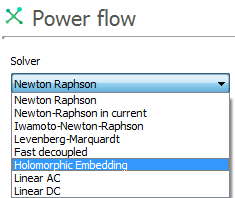
\includegraphics[scale=1.0]{Inputs/solvers2}
\caption{Mètodes resolutius del flux de potències amb què compta la versió 3.7.0 del GridCal}
\label{fig:solversGridCal}
\end{center}
\end{figure}

La formulació integrada és la formulació pròpia. També s'han inclòs els aproximants Sigma. A l'apartat de treballs futurs de les conclusions es contemplen altres funcionalitats a incorporar.



\chapter{RESULTATS AMB XARXES DE TEST INICIALS}
%treure resultats del GS i dir que no es farà servir perquè és lent, està estudiat i avui en dia es troba en desús. No posar-lo a cap taula.

Per validar el mètode d'incrustació holomòrfica i esbrinar les seves diferències respecte als mètodes tradicionals, s'han seleccionat sis xarxes de test: un sistema d'11 busos mal condicionat, les xarxes IEEE14, IEEE30 i IEEE118, el sistema Nord Pool de 44 busos i la xarxa PEGASE2869 de 2.869 busos. En aquest capítol s'estudien sense canviar el percentatge de càrrega dels busos. En el següent, es modifica la càrrega per valorar les variacions.

El sistema d'11 busos mal condicionat va ser primer plantejat per Tripathy et al. (1982). Les dades que els autors ofereixen de la topologia només contenen els elements de la matriu d'admitàncies. Bonini et al. (2015) mostren unes dades similars però més aclaridores, pel que s'utilitzen aquestes últimes. A l'hora de resoldre'l, en ser una xarxa amb relativament pocs busos, és sensat utilitzar el mètode de Gauss-Seidel. També se soluciona amb el Newton-Raphson i amb la formulació original del MIH, ja que compta amb transformadors de relació variable. Totes les potències s'han multiplicat per $\lambda=$\ 0,5 perquè de no ser així, el sistema ja des d'un principi no té solució.

La formulació pròpia del MIH també funciona per a sistemes amb transformadors de relació variable. Tanmateix, els aproximants Sigma no són representatius. Per aquest motiu, quan hi ha transformadors de relació variable d'entrada es prefereix la formulació original.

Les xarxes IEEE14, IEEE30 i IEEE 118 contenen 14, 30 i 118 busos respectivament. La primera d'elles representa una part del sistema de potència elèctric de l'Oest Mitjà dels Estats Units que data del febrer de 1962. Per la seva banda, la IEEE30 simbolitza una fracció del mateix sistema el desembre de 1961, mentre que la IEEE118 ho fa el desembre de 1962 (Christie, 2020). Els fitxers de dades s'han extret de Peñate (2020b).

Com que el sistema IEEE14 es pot considerar de dimensions reduïdes, en un principi convé utilitzar el GS, el NR i la formulació original del MIH perquè hi ha transformadors de relació variable. Per a la IEEE30 s'usa el NR i les dues formulacions del MIH. La IEEE118 es resol amb el NR i preferiblement amb la formulació original del MIH.

La xarxa Nord Pool de 44 busos es correspon a un model del sistema de transport que transcorre per Suècia, Noruega i Finlàndia. Se soluciona amb el NR i les dues formulacions del MIH. El fitxer de dades s'ha adaptat a partir dels de Peñate (2020b).

En últim lloc, la xarxa PEGASE2869 de 2.869 busos és un sistema fictici que pretén representar amb exactitud la mida i la complexitat d'una part de la xarxa europea (Zimmerman et al. 2011). També s'ha partit de les dades de Peñate (2020b). Interessa extreure resultats amb la formulació original del MIH i amb el NR. En aquest cas, més que dur a terme un estudi detallat, es vol mostrar que el MIH és capaç de resoldre un sistema de tants busos.

Cal afegir que en tots els sistemes en què s'utilitza el Newton-Raphson també s'obté la solució amb el desacoblat ràpid. S'empra el NR bàsic, però si no convergeix, s'opta pel multiplicador d'Iwamoto i pel mètode de Levenberg-Marquardt. Per aquests mètodes iteratius es fa servir el GridCal.

\section{Diagnòstic} % sigma, algun domb-sykes pels radis i justificar si cal continuació
En primer lloc es vol determinar l'estat de càrrega global de les xarxes sense introduir canvis en els consums. Els gràfics Sigma permeten donar una idea qualitativa del sistema on en conjunt s'aprecia si la demanda de potència activa i reactiva té molt pes. Si els punts es concentren al voltant del punt (0, 0) del gràfic, significa que la xarxa treballa lluny dels límits. A més, els aproximants Sigma quantifiquen si la solució és correcta, cosa que també es representa al gràfic. 

A la Figura \ref{fig:RES1} es copsen els gràfics Sigma de les xarxes de menor dimensió. D'ara endavant s'hi dibuixen les línies que indiquen que la proporció de tensió amb la de l'oscil·lant és igual a 0,9 i 1,1, de mode que visualment s'entén entre quines franges es troben els busos. 

  \begin{figure}[!ht] \footnotesize
    \begin{center}
    \begin{tikzpicture}

    \begin{groupplot}[group style={group size=2 by 1, horizontal sep=3cm}]
      \nextgroupplot[/pgf/number format/.cd, use comma, 1000 sep={.},  title={Sistema d'11 busos}, ylabel={$\sigma_{im}$},xlabel={$\sigma_{re}$},domain=-0.25:1.5,ylabel style={rotate=-90},legend style={at={(0,1)},anchor=north west},width=7cm,height=7cm,scatter/classes={a={mark=x,mark size=2pt,draw=black}, b={mark=*,mark size=2pt,draw=black}, c={mark=o,mark size=1pt,draw=black},d={mark=diamond,mark size=2pt,draw=black}, e={mark=+,mark size=2pt,draw=black}, f={mark=triangle,mark size=2pt,draw=black}}]]

    \addplot[no marks] {(0.25+\x)^(1/2)};
    \addplot[no marks] {-(0.25+\x)^(1/2)};
    \addplot[no marks, densely dashed] {+(1.1^2-(\x - 1.1^2)^2)^(1/2)};
    \addplot[no marks, densely dashed] {-(1.1^2-(\x - 1.1^2)^2)^(1/2)};
    \addplot[no marks, densely dashdotted] {+(0.9^2-(\x - 0.9^2)^2)^(1/2)};
    \addplot[no marks, densely dashdotted] {-(0.9^2-(\x - 0.9^2)^2)^(1/2)};
    \addplot[scatter, only marks,scatter src=explicit symbolic]%
        table[x = x, y = y, meta = label, col sep=semicolon] {Inputs/Resultats_inici/sig_cas11.csv};
        \legend{ , , {$V_x=$1,1}, ,{$V_x=$0,9}} %tocar
    \nextgroupplot[/pgf/number format/.cd, use comma, 1000 sep={.}, title={IEEE14}, ylabel={$\sigma_{im}$},xlabel={$\sigma_{re}$},domain=-0.25:0.25,ylabel style={rotate=-90},legend style={at={(0,1)},anchor=north west},width=7cm,height=7cm,scatter/classes={a={mark=x,mark size=2pt,draw=black}, b={mark=*,mark size=2pt,draw=black}, c={mark=o,mark size=1pt,draw=black},d={mark=diamond,mark size=2pt,draw=black}, e={mark=+,mark size=2pt,draw=black}, f={mark=triangle,mark size=2pt,draw=black}}]]

    \addplot[no marks] {(0.25+\x)^(1/2)};
    \addplot[no marks] {-(0.25+\x)^(1/2)};
    \addplot[no marks, densely dashed] {+(1.1^2-(\x - 1.1^2)^2)^(1/2)};
    \addplot[no marks, densely dashed] {-(1.1^2-(\x - 1.1^2)^2)^(1/2)};
    \addplot[no marks, densely dashdotted] {+(0.9^2-(\x - 0.9^2)^2)^(1/2)};
    \addplot[no marks, densely dashdotted] {-(0.9^2-(\x - 0.9^2)^2)^(1/2)};
    \addplot[scatter, only marks,scatter src=explicit symbolic]%
        table[x = x, y = y, meta = label, col sep=semicolon] {Inputs/Resultats_inici/sig_IEEE14.csv};
        \legend{ , , {$V_x=$1,1}, ,{$V_x=$0,9}} %tocar
    \end{groupplot}
    \end{tikzpicture}
    \caption{Gràfic Sigma del sistema d'11 busos i de la IEEE14}
    \label{fig:RES1}
    \end{center}
  \end{figure}

La xarxa IEEE14 presenta una distribució de punts típica d'un sistema ben condicionat. Tots els busos es troben entre les marques de 0,9 i 1,1. A més, no es distancien gaire del punt (0, 0). 

Per la seva banda, el sistema d'11 busos és en essència un sistema mal condicionat. Compta amb un total de set línies de transmissió i set transformadors, tots ells de relació variable. Aquestes relacions de transformació estan ajustades per sota la unitat, el que comporta que les tensions de quatre busos siguin superiors a 1,1 vegades la del bus oscil·lant, tal com s'observa a la Figura \ref{fig:RES1}. El perfil de tensions del sistema és anormal perquè si bé alguns voltatges es troben al voltant de la unitat, el bus 10 es troba a una tensió d'1,759. 

La Figura \ref{fig:RES2} mostra els gràfics Sigma per les altres xarxes: la IEEE30, la Nord Pool, la IEEE118 i la PEGASE2869. 

\begin{figure}[!ht] \footnotesize
  \begin{center}
  \begin{tikzpicture}

  \begin{groupplot}[group style={group size=2 by 2, horizontal sep=3cm, vertical sep = 1.8cm}]
    \nextgroupplot[/pgf/number format/.cd, use comma, 1000 sep={.},  title={IEEE30}, ylabel={$\sigma_{im}$},xlabel={$\sigma_{re}$},domain=-0.25:0.25,ylabel style={rotate=-90},legend style={at={(0,1)},anchor=north west},width=7cm,height=7cm,scatter/classes={a={mark=x,mark size=2pt,draw=black}, b={mark=*,mark size=2pt,draw=black}, c={mark=o,mark size=1pt,draw=black},d={mark=diamond,mark size=2pt,draw=black}, e={mark=+,mark size=2pt,draw=black}, f={mark=triangle,mark size=2pt,draw=black}}]]

  \addplot[no marks] {(0.25+\x)^(1/2)};
  \addplot[no marks] {-(0.25+\x)^(1/2)};
  \addplot[no marks, densely dashed] {+(1.1^2-(\x - 1.1^2)^2)^(1/2)};
  \addplot[no marks, densely dashed] {-(1.1^2-(\x - 1.1^2)^2)^(1/2)};
  \addplot[no marks, densely dashdotted] {+(0.9^2-(\x - 0.9^2)^2)^(1/2)};
  \addplot[no marks, densely dashdotted] {-(0.9^2-(\x - 0.9^2)^2)^(1/2)};
  \addplot[scatter, only marks,scatter src=explicit symbolic]%
      table[x = x, y = y, meta = label, col sep=semicolon] {Inputs/Resultats_inici/sig_IEEE30.csv};
      \legend{ , , {$V_x=$1,1}, ,{$V_x=$0,9}} %tocar
  \nextgroupplot[/pgf/number format/.cd, use comma, 1000 sep={.}, title={Nord Pool}, ylabel={$\sigma_{im}$},xlabel={$\sigma_{re}$},domain=-0.25:0.5,ylabel style={rotate=-90},legend style={at={(0,1)},anchor=north west},width=7cm,height=7cm,scatter/classes={a={mark=x,mark size=2pt,draw=black}, b={mark=*,mark size=2pt,draw=black}, c={mark=o,mark size=1pt,draw=black},d={mark=diamond,mark size=2pt,draw=black}, e={mark=+,mark size=2pt,draw=black}, f={mark=triangle,mark size=2pt,draw=black}}]]

  \addplot[no marks] {(0.25+\x)^(1/2)};
  \addplot[no marks] {-(0.25+\x)^(1/2)};
  \addplot[no marks, densely dashed] {+(1.1^2-(\x - 1.1^2)^2)^(1/2)};
  \addplot[no marks, densely dashed] {-(1.1^2-(\x - 1.1^2)^2)^(1/2)};
  \addplot[no marks, densely dashdotted] {+(0.9^2-(\x - 0.9^2)^2)^(1/2)};
  \addplot[no marks, densely dashdotted] {-(0.9^2-(\x - 0.9^2)^2)^(1/2)};
  \addplot[scatter, only marks,scatter src=explicit symbolic]%
      table[x = x, y = y, meta = label, col sep=semicolon] {Inputs/Resultats_inici/sig_Nord.csv};
      \legend{ , , {$V_x=$1,1}, ,{$V_x=$0,9}} %tocar
  
      \nextgroupplot[/pgf/number format/.cd, use comma, 1000 sep={.}, title={IEEE118}, ylabel={$\sigma_{im}$},xlabel={$\sigma_{re}$},domain=-0.25:0.25,ylabel style={rotate=-90},legend style={at={(0,1)},anchor=north west},width=7cm,height=7cm,scatter/classes={a={mark=x,mark size=2pt,draw=black}, b={mark=*,mark size=2pt,draw=black}, c={mark=o,mark size=1pt,draw=black},d={mark=diamond,mark size=2pt,draw=black}, e={mark=+,mark size=2pt,draw=black}, f={mark=triangle,mark size=2pt,draw=black}}]]

      \addplot[no marks] {(0.25+\x)^(1/2)};
      \addplot[no marks] {-(0.25+\x)^(1/2)};
      \addplot[no marks, densely dashed] {+(1.1^2-(\x - 1.1^2)^2)^(1/2)};
      \addplot[no marks, densely dashed] {-(1.1^2-(\x - 1.1^2)^2)^(1/2)};
      \addplot[no marks, densely dashdotted] {+(0.9^2-(\x - 0.9^2)^2)^(1/2)};
      \addplot[no marks, densely dashdotted] {-(0.9^2-(\x - 0.9^2)^2)^(1/2)};
      \addplot[scatter, only marks,scatter src=explicit symbolic]%
          table[x = x, y = y, meta = label, col sep=semicolon] {Inputs/Resultats_inici/sig_IEEE118.csv};
          \legend{ , , {$V_x=$1,1}, ,{$V_x=$0,9}} %tocar
      \nextgroupplot[/pgf/number format/.cd, use comma, 1000 sep={.}, title={PEGASE2869}, ylabel={$\sigma_{im}$},xlabel={$\sigma_{re}$},domain=-0.25:0.75,ylabel style={rotate=-90},legend style={at={(0,1)},anchor=north west},width=7cm,height=7cm,scatter/classes={a={mark=x,mark size=2pt,draw=black}, b={mark=*,mark size=2pt,draw=black}, c={mark=o,mark size=1pt,draw=black},d={mark=diamond,mark size=2pt,draw=black}, e={mark=+,mark size=2pt,draw=black}, f={mark=triangle,mark size=2pt,draw=black}}]]

      \addplot[no marks] {(0.25+\x)^(1/2)};
      \addplot[no marks] {-(0.25+\x)^(1/2)};
      \addplot[no marks, densely dashed] {+(1.1^2-(\x - 1.1^2)^2)^(1/2)};
      \addplot[no marks, densely dashed] {-(1.1^2-(\x - 1.1^2)^2)^(1/2)};
      \addplot[no marks, densely dashdotted] {+(0.9^2-(\x - 0.9^2)^2)^(1/2)};
      \addplot[no marks, densely dashdotted] {-(0.9^2-(\x - 0.9^2)^2)^(1/2)};
      \addplot[scatter, only marks,scatter src=explicit symbolic]%
          table[x = x, y = y, meta = label, col sep=semicolon] {Inputs/Resultats_inici/sig_Pegase2869.csv};
          \legend{ , , {$V_x=$1,1}, ,{$V_x=$0,9}} %tocar
  \end{groupplot}
  \end{tikzpicture}
  \caption{Gràfic Sigma de les xarxes IEEE30, Nord Pool, IEEE118 i PEGASE2869}
  \label{fig:RES2}
  \end{center}
\end{figure}

La xarxa IEEE30 es troba molt poc carregada. Tots els busos presenten mòduls de tensió molt similars. Al cap i a la fi els punts queden concentrats a prop del (0, 0). Al sistema Nord Pool els punts queden a prop de la part superior de la paràbola. Això indica que els busos en què la potència és més extrema es corresponen a busos on hi ha molta generació en lloc de molta demanda. En aquest aspecte es tracta d'un sistema anormal perquè sovint la tendència és contrària. Igual que a la xarxa IEEE30, tots els busos estan entre les línies de 0,9 i 1,1. Els seus gràfics Sigma s'han generat amb la formulació original i amb la formulació pròpia. En els dos casos resulten idèntics.

Al sistema IEEE118 altre cop tots els busos treballen entre 0,9 i 1,1 vegades el voltatge de l'oscil·lant, tot i que força més pròxims al límit de 0,9. En conjunt, s'observa que als busos PQ i PV la demanda de potència activa sobrepassa la generació, ja que els punts del gràfic tendeixen cap al límit inferior. A la xarxa PEGASE2869 el núvol de punts il·lustra que en bona part els busos també treballen dins uns marges de tensió acceptables. Tanmateix, hi ha una agrupació de punts que freguen el límit inferior. Són els més propers al col·lapse de tensions. 

Per tal d'esbrinar si els mètodes de continuació analítica són necessaris, s'estudia el radi de convergència de les sèries. S'ha comprovat que les tensions d'un mateix sistema amb una mateixa formulació presenten radis de convergència semblants. La Taula \ref{tab:radis_sist} mostra per a cada xarxa seleccionada el major i el menor radi de les tensions amb les dues formulacions. S'han definit sèries amb un total de 60 coeficients.

\begin{table}[!htb]
  \begin{center}
  \begin{tabular}{lllll}
  \hline
   Formulació & \multicolumn{2}{c}{Original} & \multicolumn{2}{c}{Pròpia} \\
   \hline
  Sistema & $r_{max}$ & $r_{min}$ & $r_{max}$ & $r_{min}$\\
  \hline
  \hline
  Cas d'11 busos & 0,882 & 0,880 & 2,838 & 2,838 \\
  IEEE14 & 3,702 & 3,679 & 4,528 & 4,513\\
  IEEE30 & 5,827 & 5,819 & 5,721 & 5,717\\
  Nord Pool & 1,917 & 1,912 & 1,881 & 1,878\\
  IEEE118 & 2,639 & 2,639 & 1,940 & 1,940\\
  PEGASE2869 & 1,460 & 1,454 & 0,808 & 0,805\\
  \hline 
  \end{tabular}
  \caption{Màxims i mínims radis de convergència de les tensions dels sistemes en l'estat inicial}
  \label{tab:radis_sist}
  \end{center}
\end{table}

Els radis de convergència de la formulació original guarden relació amb els gràfics Sigma. Per exemple, el sistema d'11 busos és on són menors. La Figura \ref{fig:RES1} ja indica una distribució de punts molt escampats. En canvi, a la IEEE30 els punts es concentren a prop del (0, 0). S'obtenen els majors radis de convergència de tots els sistemes. 

En aquesta xarxa i en la Nord Pool els radis de convergència màxims i mínims són molt similars amb les dues formulacions. No succeeix el mateix en les altres xarxes, on pot haver-hi diferències notòries. Es dedueix que una formulació pot tenir més problemes que l'altra a l'hora de solucionar el mateix sistema. En part, que una xarxa es trobi mal condicionada és relatiu a la formulació escollida.

Els resultats de la Taula \ref{tab:radis_sist} també posen de manifest que només cal emprar mètodes de continuació analítica en la xarxa PEGASE2869 amb la formulació pròpia i en el sistema d'11 busos amb l'original. En aquest sistema si se sumen els termes de tensió, el valor final no convergeix. Per exemple, la Figura \ref{fig:diagn1} mostra la tensió del bus 10 que s'aconsegueix amb els aproximants de Padé i amb la suma de coeficients depenent de la profunditat.


\begin{figure}[!ht] \footnotesize
  \begin{center}
  \begin{tikzpicture}
    \begin{axis}[/pgf/number format/.cd, use comma, 1000 sep={.}, ylabel={$|V_{10}|$},xlabel={Profunditat},domain=-0.25:1.5,ylabel style={rotate=-90},legend style={at={(1,0)},anchor=south west},width=10cm,height=7cm,scatter/classes={a={mark=x,mark size=2pt,draw=black}, b={mark=+,mark size=1.5pt,draw=black}, c={mark=o,mark size=1.5pt,draw=black},d={mark=diamond,mark size=2pt,draw=black}, e={mark=+,mark size=2pt,draw=black}, f={mark=triangle,mark size=2pt,draw=black}}]]

\addplot[scatter, scatter src=explicit symbolic]%
  table[x = x, y = y, meta = label, col sep=semicolon] {Inputs/Resultats_inici/bus10_pade2.csv};
\addplot[scatter, scatter src=explicit symbolic]%
  table[x = x, y = y, meta = label, col sep=semicolon] {Inputs/Resultats_inici/bus10_suma2.csv};
      \legend{ ,Suma, Padé} %tocar
    \end{axis}
  \end{tikzpicture}
  \caption{Evolució del mòdul de tensió del bus 10 del cas d'11 busos amb la formulació original}
  \label{fig:diagn1}
  \end{center}
\end{figure}

Encara que el valor a què s'arriba amb els aproximants de Padé és força diferent de la unitat, aconsegueixen convergir. Amb la suma de termes la solució divergeix. Com més s'incrementa la profunditat, més s'allunya la solució obtinguda amb la suma comparada amb la dels aproximants de Padé. La continuació analítica és necessària en aquesta situació.

En canvi, a la xarxa IEEE30 s'obté el perfil de la Figura \ref{fig:diagn2} per al bus 29.

\begin{figure}[!ht] \footnotesize
  \begin{center}
  \begin{tikzpicture}
    \begin{axis}[/pgf/number format/.cd, use comma, 1000 sep={.}, ylabel={$|V_{29}|$},xlabel={Profunditat},domain=-0.25:1.5,ylabel style={rotate=-90},legend style={at={(1,0)},anchor=south west},width=10cm,height=7cm,scatter/classes={a={mark=x,mark size=2pt,draw=black}, b={mark=+,mark size=1.5pt,draw=black}, c={mark=o,mark size=1.5pt,draw=black},d={mark=diamond,mark size=2pt,draw=black}, e={mark=+,mark size=2pt,draw=black}, f={mark=triangle,mark size=2pt,draw=black}}]]

\addplot[scatter, scatter src=explicit symbolic]%
  table[x = x, y = y, meta = label, col sep=semicolon] {Inputs/Resultats_inici/bus29_pade.csv};
\addplot[scatter, scatter src=explicit symbolic]%
  table[x = x, y = y, meta = label, col sep=semicolon] {Inputs/Resultats_inici/bus29_suma.csv};
      \legend{ ,Suma, Padé} %tocar
    \end{axis}
  \end{tikzpicture}
  \caption{Evolució del mòdul de tensió del bus 29 de la IEEE30 amb la formulació original}
  \label{fig:diagn2}
  \end{center}
\end{figure}

No només de les dues maneres el voltatge convergeix, sinó que en tractar-se d'un sistema ben condicionat, ho fa força a major velocitat en comparació amb el cas d'11 busos. Pràcticament a cada profunditat el mòdul resultant de tensió coincideix, pel que gairebé no s'aprecien les diferències entre l'evolució del voltatge amb la suma o amb els aproximants de Padé.

\section{Comparació amb mètodes tradicionals}
Una eina com els aproximants Sigma i el seu gràfic són útils per determinar a simple cop d'ull l'estat d'operació del sistema. No obstant això, són propis del mètode d'incrustació holomòrfica. Atès que els mètodes iteratius com el Gauss-Seidel, el Newton-Raphson i el desacoblat ràpid per definició no compten amb aquest recurs, es procedeix a solucionar els sistemes per primer comprovar que s'obté la solució, i en segon lloc, per tal de descobrir si d'algun mode s'intueix que les xarxes es troben mal condicionades.

A la Taula \ref{tab:solucio_iteratius1} es captura l'error màxim així com el nombre d'iteracions necessari per a cada sistema amb els mètodes iteratius esmentats. S'ha fixat un error màxim de $10^{-10}$ amb els resultats del NR i del FDLF. Pel GS, que se soluciona amb el PowerWorld, s'assumeix que l'error màxim és de $10^{-6}$ perquè no indica més decimals. Per tant, no hi ha interès en l'error.

\begin{table}[!htb]
  \begin{center}
  \begin{tabular}{llllll}
  \hline
   & \multicolumn{2}{c}{Errors} & \multicolumn{3}{c}{Iteracions} \\
  \hline
  Sistema & NR & FDLF & GS & NR & FDLF\\
  \hline
  \hline
  Cas d'11 busos & 2,94.10$^{-12}$ & 8,28.10$^{-11}$ & 282 & 7 & 80\\
  IEEE14 & 8,86.10$^{-16}$& 6,90.10$^{-11}$ & 180 & 3 & 22\\
  IEEE30 & 4,48.10$^{-17}$ & 9,52.10$^{-11}$ & - & 3 & 22\\
  Nord Pool & 9,93.10$^{-11}$ & 7,21.10$^{-11}$ & - & 3 & 20\\
  IEEE118 & 3,93.10$^{-12}$ & 2,64.10$^{-11}$ & - & 3 & 14\\
  PEGASE2869 & 3,25.10$^{-16}$ & 8,96.10$^{-11}$ & - & 6 & 70\\ 
  \hline 
  \end{tabular}
  \caption{Errors obtinguts i iteracions necessàries en els sis sistemes seleccionats}
  \label{tab:solucio_iteratius1}
  \end{center}
\end{table}

A partir de la Taula \ref{tab:solucio_iteratius1} s'observa que encara que hi hagi pocs busos, el GS requereix moltes iteracions pel cas d'11 busos i per la IEEE14. Es tracta d'un mètode amb poca utilitat per resoldre fluxos de potència que segons Kothari i Nagrath (2011) resulta menys fiable que el NR. D'ara endavant no serà utilitzat.

El mètode de NR bàsic és el que menys iteracions necessita. Per la majoria de sistemes només n'hi fan falta 3 gràcies a la seva convergència quadràtica. A la xarxa PEGASE2869 itera 6 vegades, segurament a causa de la seva dimensió. Per contra, el cas d'11 busos, tot i ser el de menors dimensions, demana més iteracions que la resta de sistemes. Això dóna a pensar que es tracta d'un sistema mal condicionat. Aparentment en cap cas cal recórrer al multiplicador d'Iwamoto o al mètode de Levenberg-Marquardt perquè el NR bàsic convergeix i aconsegueix l'error desitjat.

Per altra banda, teòricament el FDLF necessita més iteracions que el NR però menys que el GS. Com s'aprecia a la Taula \ref{tab:solucio_iteratius1}, altre cop al cas d'11 busos és on es requereixen més iteracions. 

El cas d'11 busos mereix especial atenció. Encara que s'hagi reduït la càrrega a la meitat, es troba que amb el NR la solució convergeix a unes tensions extremadament baixes que corresponen a solucions que formen part de la branca inestable de la corba PV. A la Taula \ref{tab:modulcas11} es plasmen els mòduls de tensió obtinguts amb el NR bàsic, el FDLF i les variacions del NR com el multiplicador d'Iwamoto i el mètode de Levenberg-Marquardt (L-M). També hi apareixen els voltatges obtinguts amb les dues formulacions del MIH. Se segueix la nomenclatura dels busos tal com apareixen als fitxers de dades del MIH.

\begin{table}[!htb]
  \begin{center}
  \begin{tabular}{lllllll}
  \hline
  Bus & NR & FDLF & NR Iwamoto & NR L-M & MIH propi & MIH original\\
  \hline
  \hline
  0 & 1,024 & 1,024& 1,024 & 1,024 & 1,024 & 1,024\\
  1 & 1,047 & 1,080 & 1,047 & 1,080 & 1,080 & 1,080\\
  2 & 1,041 & 1,080& 1,041 & 1,080 & 1,080 & 1,080\\
  3 & 1,014 & 1,073 & 1,014 & 1,073& 1,073 & 1,073\\
  4 & 1,035 & 1,080& 1,035 & 1,080& 1,080 & 1,080\\
  5 & 1,034 & 1,094 & 1,034 &1,094 & 1,094 & 1,094\\
  6 & 0,536 & 1,088 & 0,536 &1,088 & 1,088 & 1,088\\
  7 & 0,512 & 1,302 & 0,512 & 1,302& 1,302 & 1,302\\
  8 & 0,665 & 1,709 & 0,665 &1,709 & 1,709 & 1,709\\
  9 & 0,260 & 1,322 & 0,260 &1,322 & 1,322 & 1,322\\
  10 & 0,290 & 1,759 &0,290 &1,759 & 1,759&1,759 \\
  \hline 
  \end{tabular}
  \caption{Mòdul de tensions del cas d'11 busos amb mètodes iteratius i amb MIH}
  \label{tab:modulcas11}
  \end{center}
\end{table}

Per una banda, el FDLF, el NR amb Levenberg-Marquardt i les dues formulacions del MIH porten a la mateixa solució. S'observa que tot i haver-hi transformadors de relació variable, els dos plantejaments del mètode d'incrustació holomòrfica arriben a voltatges idèntics. Les tensions dels darrers busos prenen valors molt distants de la unitat, el que provoca que el perfil de tensions en conjunt sigui anormal. De fet, guarda relació amb les relacions de transformació variable. Totes elles estan ajustades a valors per sota la unitat. Així, intuïtivament s'entén que les tensions dels busos PQ superin la del bus oscil·lant de bastant. 

Per altra banda, el NR bàsic i el NR amb el multiplicador d'Iwamoto arriben a una solució que encara que matemàticament és possible, correspon a la tensió de la branca negativa o inestable de les corbes PV. Per confirmar això, la Taula \ref{tab:modulcas11thx} recull els mòduls de voltatge calculats amb els aproximants de Thévenin per una profunditat de 60 i les solucions del NR bàsic. 

\begin{table}[!htb]
\begin{center}
  \begin{tabular}{lll}
  \hline
  Bus & NR & Thévenin\\
  \hline
  \hline
  0 & 1,024 & -\\
  1 & 1,047 & 1,042\\
  2 & 1,041 & 1,043\\
  3 & 1,014 & 1,009\\
  4 & 1,035 & 1,042\\
  5 & 1,034 & 1,036\\
  6 & 0,536 & 0,539\\
  7 & 0,512 & 0,510\\
  8 & 0,665 & 0,670\\
  9 & 0,260 & 0,259\\
  10 & 0,290 & 0,291\\
  \hline 
  \end{tabular}
  \caption{Mòdul de tensions del cas d'11 busos amb NR i amb aproximants de Thévenin}
  \label{tab:modulcas11thx}
  \end{center}
\end{table}

Els aproximants de Thévenin no s'utilitzen per al voltatge del bus oscil·lant, atès que es tracta d'una dada. Per la resta de busos hi ha alguna diferència de decimals, però en general les dues solucions s'assimilen molt. 

Segons Tripathy et al. (1982), el cas d'11 busos correspon a un sistema mal condicionat, no necessàriament perquè la càrrega sigui excessiva. Sense canviar els percentatges de càrrega, el van trobar divergent tant pel NR com pel FDLF. Justifiquen que el jacobià presenta un nombre de condició elevat. En el problema del flux de potències, el nombre de condició representa com varien les incògnites si el vector que conté els errors de potència canvia lleugerament. Un gran nombre de condició complica l'obtenció de la solució.

El cas d'11 busos il·lustra la problemàtica de fer servir el mètode de Newton-Raphson. En un sistema mal condicionat el mètode pot convergir cap a una solució inestable que durant condicions d'operació normals no es donarà. Per contra, algunes de les seves variacions (com el FDLF i el NR L-M) assoleixen la solució correcta des del punt de vista d'operació del sistema. Conèixer el sistema permet fer-se una idea aproximada de la correcció de la solució, però no hi ha eines per confirmar-ho.

Contrari als mètodes iteratius, el MIH genera un gràfic Sigma que indica que tots els punts es troben dins la paràbola, i per tant, la solució és correcta. A més, els aproximants de Thévenin obtenen tant la solució corresponent a la branca estable de la corba PV com la de la inestable. Tal riquesa d'eines no està present en els mètodes iteratius. Com s'ha vist, el sistema no es pot conèixer tan a fons.

\section{Influència de la profunditat}
Igual que l'evolució de l'error en els mètodes iteratius depèn del nombre d'iteracions, en el MIH el nombre de coeficients que constitueixen les sèries també afecta el resultat final. S'espera que a més coeficients, millor es construirà la solució. 

Primer es busca determinar si hi ha diferències notables entre l'error i la profunditat en les dues formulacions del MIH. Se selecciona el cas d'11 busos perquè a part d'estar mal condicionat, compta amb diversos transformadors de relació variable. Per definició la formulació pròpia del MIH no és encertada per calcular els aproximants Sigma. Tanmateix, a diferència de la formulació original, no fragmenta la matriu d'admitàncies total en simètrica amb totes les files que sumen 0 i en asimètrica on la suma de totes les files no resulta nul·la. L'evolució de l'error calculat amb Padé segons la profunditat es mostra a la Figura \ref{fig:err2formul}.

\begin{figure}[!ht] \footnotesize
  \begin{center}
  \begin{tikzpicture}
    \begin{axis}[/pgf/number format/.cd, use comma, 1000 sep={.}, ylabel={$\log |\Delta S_{max}|$},xlabel={Profunditat},domain=-0.25:1.5,ylabel style={rotate=-90},legend style={at={(1,0)},anchor=south west},width=10cm,height=7cm,scatter/classes={a={mark=x,mark size=2pt,draw=black}, b={mark=*,mark size=2pt,draw=black}, c={mark=o,mark size=2pt,draw=black},d={mark=diamond,mark size=2pt,draw=black}, e={mark=+,mark size=2pt,draw=black}, f={mark=triangle,mark size=2pt,draw=black}}]]

\addplot[scatter, scatter src=explicit symbolic]%
  table[x = x, y = y, meta = label, col sep=semicolon] {Inputs/Resultats_inici/prof11_propi.csv};
\addplot[scatter, scatter src=explicit symbolic]%
  table[x = x, y = y, meta = label, col sep=semicolon] {Inputs/Resultats_inici/prof11_original.csv};
      \legend{ ,Pròpia, Original} %tocar
    \end{axis}
  \end{tikzpicture}
  \caption{Evolució del logaritme de l'error màxim pel cas d'11 busos amb les dues formulacions}
  \label{fig:err2formul}
  \end{center}
\end{figure}

La formulació pròpia no força que els primers coeficients de les sèries de tensió siguin tots 1. Això per una banda impossibilita l'ús dels aproximants Sigma, però aconsegueix que aquests primers coeficients s'acostin molt més a la solució final. Amb qüestió de 20 coeficients s'arriba a un error de l'ordre de 10$^{-14}$. A partir d'aquest punt, incrementar la profunditat no millora significativament l'error. De fet, el radi de convergència de les sèries amb la formulació pròpia és de 2,838, molt superior al de la formulació original. Per això, amb aquesta calen força més coeficients per assolir un error satisfactori de l'ordre de 10$^{-10}$.

En altres sistemes on les relacions de transformació variables s'ajusten més a la unitat i no són tan nombroses, les dues formulacions segueixen una progressió de l'error en funció la profunditat similar. La Figura \ref{fig:err2formul2} ho exemplifica per la IEEE118. També s'utilitzen els aproximants de Padé. Tal com s'observa, malgrat que els radis de convergència difereixin, les dues formulacions esdevenen competitives. Amb uns 20 coeficients l'error s'estabilitza.

\begin{figure}[!ht] \footnotesize
  \begin{center}
  \begin{tikzpicture}
    \begin{axis}[/pgf/number format/.cd, use comma, 1000 sep={.}, ylabel={$\log |\Delta S_{max}|$},xlabel={Profunditat},domain=-0.25:1.5,ylabel style={rotate=-90},legend style={at={(1,0)},anchor=south west},width=10cm,height=7cm,scatter/classes={a={mark=x,mark size=2pt,draw=black}, b={mark=*,mark size=2pt,draw=black}, c={mark=o,mark size=2pt,draw=black},d={mark=diamond,mark size=2pt,draw=black}, e={mark=+,mark size=2pt,draw=black}, f={mark=triangle,mark size=2pt,draw=black}}]]

\addplot[scatter, scatter src=explicit symbolic]%
  table[x = x, y = y, meta = label, col sep=semicolon] {Inputs/Resultats_inici/prof118_propi.csv};
\addplot[scatter, scatter src=explicit symbolic]%
  table[x = x, y = y, meta = label, col sep=semicolon] {Inputs/Resultats_inici/prof118_original.csv};
      \legend{ ,Pròpia, Original} %tocar
    \end{axis}
  \end{tikzpicture}
  \caption{Evolució del logaritme de l'error màxim per la IEEE118 amb les dues formulacions}
  \label{fig:err2formul2}
  \end{center}
\end{figure}

Com ja s'ha esmentat, no és que la formulació pròpia no pugui solucionar les xarxes en el seu estat inicial. N'és capaç, l'únic que quan hi ha transformadors de relació variable, el gràfic Sigma que proporciona esdevé enganyós. Tant per tant val la pena utilitzar la formulació original perquè no compta amb aquesta limitació.

S'ha notat que a l'hora de resoldre el flux de potències per mitjà dels mètodes iteratius, el nombre d'iteracions requerides pel NR en general presenta poca variabilitat al costat del FDLF. Per això, també es valora la profunditat necessària de la formulació original del MIH per obtenir un error màxim de 10$^{-10}$. La Taula \ref{tab:coef_form_orig} mostra el nombre de coeficients requerits i l'error resultant pels sistemes seleccionats amb els aproximants de Padé.  

\begin{table}[!htb]
  \begin{center}
  \begin{tabular}{lll}
  \hline
  Sistema & Errors & Profunditat\\
  \hline
  \hline
  Cas d'11 busos &2,53.10$^{-11}$ & 69\\
  IEEE14 & 3,29.10$^{-11}$& 12\\
  IEEE30 & 5,52.10$^{-12}$ & 10\\
  Nord Pool & 3,70.10$^{-11}$& 21\\
  IEEE118 & 6,82.10$^{-11}$ & 16\\
  PEGASE2869 &2,36.10$^{-11}$ & 28\\ 
  \hline 
  \end{tabular}
  \caption{Errors obtinguts i profunditat necessària en els sis sistemes seleccionats amb el MIH original}
  \label{tab:coef_form_orig}
  \end{center}
\end{table}

A partir de la Taula \ref{tab:coef_form_orig} es dedueix que la profunditat requerida guarda certa relació amb els radis de convergència de la Taula \ref{tab:radis_sist}: a major radi de convergència cal menys profunditat. S'observa que en aquests exemples el nombre de busos no marca la tendència de quants coeficients fan falta. La xarxa PEGASE2869 és d'una dimensió molt superior al sistema d'11 busos, però així i tot, en aquest últim es necessita força més profunditat. De forma similar al mètode de NR, des d'un punt de vista de temps de càlcul, és interessant que el nombre de busos no tingui gaire influència en la profunditat.

El càlcul de la solució final no sempre s'ha de dur a terme amb els aproximants de Padé. Els mètodes recurrents són una alternativa vàlida, com també ho és la suma de coeficients quan no fa falta continuació analítica. 

Per tal de fer-se una idea de l'error existent en funció de la profunditat, primerament s'estudia el cas d'11 busos, ja que segons el raonat fins ara es tracta d'un sistema mal condicionat. A la Figura \ref{fig:11contin_met} apareixen els resultats amb els diversos mètodes de continuació (ja que no s'hi val a utilitzar la suma de coeficients), calculats amb la formulació original. 

Els únics mètodes que han arribat a solucions satisfactòries són els aproximants de Padé, l'Èpsilon de Wynn i l'Eta de Bauer (en aquest últim cas les potències reactives han estat calculades amb Padé). Amb la resta de mètodes les solucions no convergeixen.

\begin{figure}[!ht] \footnotesize
  \begin{center}
  \begin{tikzpicture}
    \begin{axis}[/pgf/number format/.cd, use comma, 1000 sep={.}, ylabel={$\log |\Delta S_{max}|$},xlabel={Profunditat},domain=-0.25:1.5,ylabel style={rotate=-90},legend style={at={(1,0)},anchor=south west},width=12cm,height=9cm,scatter/classes={a={mark=x,mark size=2pt,draw=black}, b={mark=*,mark size=2pt,draw=black}, c={mark=o,mark size=2pt,draw=black},d={mark=diamond,mark size=2pt,draw=black}, e={mark=+,mark size=2pt,draw=black}, f={mark=triangle*,mark size=2pt,draw=black},  g={mark=square,mark size=2pt,draw=black},  h={mark=pentagon,mark size=2pt,draw=black}}]]

\addplot[scatter, scatter src=explicit symbolic]%
table[x = x, y = y, meta = label, col sep=semicolon] {Inputs/Resultats_inici/11_eps.csv};
\addplot[scatter, scatter src=explicit symbolic]%
table[x = x, y = y, meta = label, col sep=semicolon] {Inputs/Resultats_inici/11_eta.csv};
\addplot[scatter, scatter src=explicit symbolic]%
table[x = x, y = y, meta = label, col sep=semicolon] {Inputs/Resultats_inici/11_pade.csv};

      \legend{, , , Èpsilon, , Eta, Padé} %tocar
    \end{axis}
  \end{tikzpicture}
  \caption{Evolució de l'error pel cas d'11 busos amb continuació analítica, formulació original}
  \label{fig:11contin_met}
  \end{center}
\end{figure}

Tal com s'observa, pràcticament tots tres mètodes assoleixen els mateixos errors al llarg de les diverses profunditats. De fet, a la IEEE14 amb $\lambda=2$ també es deduïa que aquests tres mètodes de continuació analítica eren els més encertats (Figura \ref{fig:err4}).

Per contra, amb la formulació pròpia s'ha vist que es necessiten menys coeficients. A part dels aproximants de Padé, la Figura \ref{fig:11contin_met2} demostra que la resta de mètodes de continuació analítica també són útils.

\begin{figure}[!ht] \footnotesize
  \begin{center}
  \begin{tikzpicture}
    \begin{axis}[/pgf/number format/.cd, use comma, 1000 sep={.}, ylabel={$\log |\Delta S_{max}|$},xlabel={Profunditat},domain=-0.25:1.5,ylabel style={rotate=-90},legend style={at={(1,0)},anchor=south west},width=12cm,height=9cm,scatter/classes={a={mark=x,mark size=2pt,draw=black}, b={mark=*,mark size=2pt,draw=black}, c={mark=o,mark size=2pt,draw=black},d={mark=diamond,mark size=2pt,draw=black}, e={mark=+,mark size=2pt,draw=black}, f={mark=triangle*,mark size=2pt,draw=black},  g={mark=square,mark size=2pt,draw=black},  h={mark=pentagon,mark size=2pt,draw=black}}]]
     
\addplot[scatter, scatter src=explicit symbolic]%
table[x = x, y = y, meta = label, col sep=semicolon] {Inputs/Resultats_inici/11_delta2.csv};      
\addplot[scatter, scatter src=explicit symbolic]%
table[x = x, y = y, meta = label, col sep=semicolon] {Inputs/Resultats_inici/11_shanks2.csv};
\addplot[scatter, scatter src=explicit symbolic]%
table[x = x, y = y, meta = label, col sep=semicolon] {Inputs/Resultats_inici/11_rho2.csv};     
\addplot[scatter, scatter src=explicit symbolic]%
table[x = x, y = y, meta = label, col sep=semicolon] {Inputs/Resultats_inici/11_eps2.csv};
\addplot[scatter, scatter src=explicit symbolic]%
table[x = x, y = y, meta = label, col sep=semicolon] {Inputs/Resultats_inici/11_theta2.csv};
\addplot[scatter, scatter src=explicit symbolic]%
table[x = x, y = y, meta = label, col sep=semicolon] {Inputs/Resultats_inici/11_eta3.csv};
\addplot[scatter, scatter src=explicit symbolic]%
table[x = x, y = y, meta = label, col sep=semicolon] {Inputs/Resultats_inici/11_pade3.csv};
\addplot[scatter, scatter src=explicit symbolic]%
table[x = x, y = y, meta = label, col sep=semicolon] {Inputs/Resultats_inici/11_suma2.csv};

      \legend{Delta, Shanks (x3), Rho, Èpsilon, Theta, Eta, Padé, Suma} %tocar
    \end{axis}
  \end{tikzpicture}
  \caption{Evolució de l'error pel cas d'11 busos, formulació pròpia}
  \label{fig:11contin_met2}
  \end{center}
\end{figure}

De tots els mètodes de continuació analítica, el Rho de Wynn són la pitjor opció. Convergeix més lentament que la resta. L'Eta de Bauer, l'Èpsilon de Wynn i els aproximants de Padé es tornen a perfilar com els mètodes que presenten menys error a la llarga. Un grup intermedi està constituït per les tres transformacions de Shanks, el mètode Theta de Brezinski i el Delta d'Aitken. Donat que el radi de convergència de les sèries és superior a 1 amb la formulació pròpia, la suma de termes també proporciona errors satisfactoris.

Es torna a realitzar la mateixa comparació per un sistema més ben condicionat com és la IEEE30. En aquest cas s'utilitza la formulació original. Com que no hi ha transformadors de relació variable, les diferències entre ambdues formulacions són poc apreciables. La Figura \ref{fig:30contin_met3} mostra l'evolució de l'error màxim segons la profunditat. També es contempla la suma de coeficients, que tal com indica el seu radi de convergència, es tracta d'una opció viable.

\begin{figure}[!ht] \footnotesize
  \begin{center}
  \begin{tikzpicture}
    \begin{axis}[/pgf/number format/.cd, use comma, 1000 sep={.}, ylabel={$\log |\Delta S_{max}|$},xlabel={Profunditat},domain=-0.25:1.5,ylabel style={rotate=-90},legend style={at={(1,0)},anchor=south west},width=12cm,height=9cm,scatter/classes={a={mark=x,mark size=2pt,draw=black}, b={mark=*,mark size=2pt,draw=black}, c={mark=o,mark size=2pt,draw=black},d={mark=diamond,mark size=2pt,draw=black}, e={mark=+,mark size=2pt,draw=black}, f={mark=triangle,mark size=2pt,draw=black},  g={mark=square,mark size=2pt,draw=black},  h={mark=pentagon,mark size=2pt,draw=black}}]]
     
\addplot[scatter, scatter src=explicit symbolic]%
table[x = x, y = y, meta = label, col sep=semicolon] {Inputs/Resultats_inici/30_delta3.csv};      
\addplot[scatter, scatter src=explicit symbolic]%
table[x = x, y = y, meta = label, col sep=semicolon] {Inputs/Resultats_inici/30_shanks3.csv};
\addplot[scatter, scatter src=explicit symbolic]%
table[x = x, y = y, meta = label, col sep=semicolon] {Inputs/Resultats_inici/30_rho3.csv};     
\addplot[scatter, scatter src=explicit symbolic]%
table[x = x, y = y, meta = label, col sep=semicolon] {Inputs/Resultats_inici/30_eps3.csv};
\addplot[scatter, scatter src=explicit symbolic]%
table[x = x, y = y, meta = label, col sep=semicolon] {Inputs/Resultats_inici/30_theta3.csv};
\addplot[scatter, scatter src=explicit symbolic]%
table[x = x, y = y, meta = label, col sep=semicolon] {Inputs/Resultats_inici/30_pade3.csv};
\addplot[scatter, scatter src=explicit symbolic]%
table[x = x, y = y, meta = label, col sep=semicolon] {Inputs/Resultats_inici/30_suma3.csv};

      \legend{Delta, Shanks (x3), Rho, Èpsilon, Theta, , Padé, Suma} %tocar
    \end{axis}
  \end{tikzpicture}
  \caption{Evolució de l'error per la IEEE30, formulació original}
  \label{fig:30contin_met3}
  \end{center}
\end{figure}

Amb presència de busos PV, si es fa servir la formulació original, el primer terme de les incògnites de potències reactives és nul. Per això és preferible no trobar la solució amb Eta; altrament té lloc una divisió per 0. Si tot i això es vol utilitzar Eta, un recurs consisteix a fer un híbrid: les tensions es calculen amb Eta i les potències reactives amb Padé, tal com s'ha fet a la Figura \ref{fig:11contin_met}. Aquesta vegada els aproximants de Padé resulten la millor eina per computar la solució final. Sumar els coeficients també proporciona errors competitius, normalment millors que amb Èpsilon fins i tot. El mètode de Rho de Wynn torna a ser el més desafavorit.

Per altra banda, els aproximants Sigma són sèries, i com a tal, depenen del nombre de coeficients triat. Les Figures \ref{fig:RES1} i \ref{fig:RES2} han sigut generades a partir de 60 coeficients. Si en lloc de 60 se n'escullen 10, que és una profunditat en què els errors encara tenen marge de millora, s'obté la Figura \ref{fig:RES3X}.


\begin{figure}[!ht] \footnotesize
  \begin{center}
  \begin{tikzpicture}

  \begin{groupplot}[group style={group size=2 by 3, horizontal sep=3cm, vertical sep = 1.8cm}]
    \nextgroupplot[/pgf/number format/.cd, use comma, 1000 sep={.},  title={Sistema d'11 busos}, ylabel={$\sigma_{im}$},xlabel={$\sigma_{re}$},domain=-0.25:3.0,ylabel style={rotate=-90},legend style={at={(0,1)},anchor=north west},width=7cm,height=7cm,scatter/classes={a={mark=x,mark size=2pt,draw=black}, b={mark=*,mark size=2pt,draw=black}, c={mark=o,mark size=1pt,draw=black},d={mark=diamond,mark size=2pt,draw=black}, e={mark=+,mark size=2pt,draw=black}, f={mark=triangle,mark size=2pt,draw=black}}]]

  \addplot[no marks] {(0.25+\x)^(1/2)};
  \addplot[no marks] {-(0.25+\x)^(1/2)};
  \addplot[no marks, densely dashed] {+(1.1^2-(\x - 1.1^2)^2)^(1/2)};
  \addplot[no marks, densely dashed] {-(1.1^2-(\x - 1.1^2)^2)^(1/2)};
  \addplot[no marks, densely dashdotted] {+(0.9^2-(\x - 0.9^2)^2)^(1/2)};
  \addplot[no marks, densely dashdotted] {-(0.9^2-(\x - 0.9^2)^2)^(1/2)};
  \addplot[scatter, only marks,scatter src=explicit symbolic]%
      table[x = x, y = y, meta = label, col sep=semicolon] {Inputs/Resultats_inici/sig2_cas11.csv};
      \legend{ , , {$V_x=$1,1}, ,{$V_x=$0,9}} %tocar

      \nextgroupplot[/pgf/number format/.cd, use comma, 1000 sep={.},  title={IEEE14}, ylabel={$\sigma_{im}$},xlabel={$\sigma_{re}$},domain=-0.25:0.25,ylabel style={rotate=-90},legend style={at={(0,1)},anchor=north west},width=7cm,height=7cm,scatter/classes={a={mark=x,mark size=2pt,draw=black}, b={mark=*,mark size=2pt,draw=black}, c={mark=o,mark size=1pt,draw=black},d={mark=diamond,mark size=2pt,draw=black}, e={mark=+,mark size=2pt,draw=black}, f={mark=triangle,mark size=2pt,draw=black}}]]

  \addplot[no marks] {(0.25+\x)^(1/2)};
  \addplot[no marks] {-(0.25+\x)^(1/2)};
  \addplot[no marks, densely dashed] {+(1.1^2-(\x - 1.1^2)^2)^(1/2)};
  \addplot[no marks, densely dashed] {-(1.1^2-(\x - 1.1^2)^2)^(1/2)};
  \addplot[no marks, densely dashdotted] {+(0.9^2-(\x - 0.9^2)^2)^(1/2)};
  \addplot[no marks, densely dashdotted] {-(0.9^2-(\x - 0.9^2)^2)^(1/2)};
  \addplot[scatter, only marks,scatter src=explicit symbolic]%
      table[x = x, y = y, meta = label, col sep=semicolon] {Inputs/Resultats_inici/sig2_IEEE14.csv};
      \legend{ , , {$V_x=$1,1}, ,{$V_x=$0,9}} %tocar

    \nextgroupplot[/pgf/number format/.cd, use comma, 1000 sep={.},  title={IEEE30}, ylabel={$\sigma_{im}$},xlabel={$\sigma_{re}$},domain=-0.25:0.25,ylabel style={rotate=-90},legend style={at={(0,1)},anchor=north west},width=7cm,height=7cm,scatter/classes={a={mark=x,mark size=2pt,draw=black}, b={mark=*,mark size=2pt,draw=black}, c={mark=o,mark size=1pt,draw=black},d={mark=diamond,mark size=2pt,draw=black}, e={mark=+,mark size=2pt,draw=black}, f={mark=triangle,mark size=2pt,draw=black}}]]

  \addplot[no marks] {(0.25+\x)^(1/2)};
  \addplot[no marks] {-(0.25+\x)^(1/2)};
  \addplot[no marks, densely dashed] {+(1.1^2-(\x - 1.1^2)^2)^(1/2)};
  \addplot[no marks, densely dashed] {-(1.1^2-(\x - 1.1^2)^2)^(1/2)};
  \addplot[no marks, densely dashdotted] {+(0.9^2-(\x - 0.9^2)^2)^(1/2)};
  \addplot[no marks, densely dashdotted] {-(0.9^2-(\x - 0.9^2)^2)^(1/2)};
  \addplot[scatter, only marks,scatter src=explicit symbolic]%
      table[x = x, y = y, meta = label, col sep=semicolon] {Inputs/Resultats_inici/sig2_IEEE30.csv};
      \legend{ , , {$V_x=$1,1}, ,{$V_x=$0,9}} %tocar
  \nextgroupplot[/pgf/number format/.cd, use comma, 1000 sep={.}, title={Nord Pool}, ylabel={$\sigma_{im}$},xlabel={$\sigma_{re}$},domain=-0.25:0.5,ylabel style={rotate=-90},legend style={at={(0,1)},anchor=north west},width=7cm,height=7cm,scatter/classes={a={mark=x,mark size=2pt,draw=black}, b={mark=*,mark size=2pt,draw=black}, c={mark=o,mark size=1pt,draw=black},d={mark=diamond,mark size=2pt,draw=black}, e={mark=+,mark size=2pt,draw=black}, f={mark=triangle,mark size=2pt,draw=black}}]]

  \addplot[no marks] {(0.25+\x)^(1/2)};
  \addplot[no marks] {-(0.25+\x)^(1/2)};
  \addplot[no marks, densely dashed] {+(1.1^2-(\x - 1.1^2)^2)^(1/2)};
  \addplot[no marks, densely dashed] {-(1.1^2-(\x - 1.1^2)^2)^(1/2)};
  \addplot[no marks, densely dashdotted] {+(0.9^2-(\x - 0.9^2)^2)^(1/2)};
  \addplot[no marks, densely dashdotted] {-(0.9^2-(\x - 0.9^2)^2)^(1/2)};
  \addplot[scatter, only marks,scatter src=explicit symbolic]%
      table[x = x, y = y, meta = label, col sep=semicolon] {Inputs/Resultats_inici/sig2_Nord.csv};
      \legend{ , , {$V_x=$1,1}, ,{$V_x=$0,9}} %tocar
  
      \nextgroupplot[/pgf/number format/.cd, use comma, 1000 sep={.}, title={IEEE118}, ylabel={$\sigma_{im}$},xlabel={$\sigma_{re}$},domain=-0.25:0.25,ylabel style={rotate=-90},legend style={at={(0,1)},anchor=north west},width=7cm,height=7cm,scatter/classes={a={mark=x,mark size=2pt,draw=black}, b={mark=*,mark size=2pt,draw=black}, c={mark=o,mark size=1pt,draw=black},d={mark=diamond,mark size=2pt,draw=black}, e={mark=+,mark size=2pt,draw=black}, f={mark=triangle,mark size=2pt,draw=black}}]]

      \addplot[no marks] {(0.25+\x)^(1/2)};
      \addplot[no marks] {-(0.25+\x)^(1/2)};
      \addplot[no marks, densely dashed] {+(1.1^2-(\x - 1.1^2)^2)^(1/2)};
      \addplot[no marks, densely dashed] {-(1.1^2-(\x - 1.1^2)^2)^(1/2)};
      \addplot[no marks, densely dashdotted] {+(0.9^2-(\x - 0.9^2)^2)^(1/2)};
      \addplot[no marks, densely dashdotted] {-(0.9^2-(\x - 0.9^2)^2)^(1/2)};
      \addplot[scatter, only marks,scatter src=explicit symbolic]%
          table[x = x, y = y, meta = label, col sep=semicolon] {Inputs/Resultats_inici/sig2_IEEE118.csv};
          \legend{ , , {$V_x=$1,1}, ,{$V_x=$0,9}} %tocar
      \nextgroupplot[/pgf/number format/.cd, use comma, 1000 sep={.}, title={PEGASE2869}, ylabel={$\sigma_{im}$},xlabel={$\sigma_{re}$},domain=-0.25:0.75,ylabel style={rotate=-90},legend style={at={(0,1)},anchor=north west},width=7cm,height=7cm,scatter/classes={a={mark=x,mark size=2pt,draw=black}, b={mark=*,mark size=2pt,draw=black}, c={mark=o,mark size=1pt,draw=black},d={mark=diamond,mark size=2pt,draw=black}, e={mark=+,mark size=2pt,draw=black}, f={mark=triangle,mark size=2pt,draw=black}}]]

      \addplot[no marks] {(0.25+\x)^(1/2)};
      \addplot[no marks] {-(0.25+\x)^(1/2)};
      \addplot[no marks, densely dashed] {+(1.1^2-(\x - 1.1^2)^2)^(1/2)};
      \addplot[no marks, densely dashed] {-(1.1^2-(\x - 1.1^2)^2)^(1/2)};
      \addplot[no marks, densely dashdotted] {+(0.9^2-(\x - 0.9^2)^2)^(1/2)};
      \addplot[no marks, densely dashdotted] {-(0.9^2-(\x - 0.9^2)^2)^(1/2)};
      \addplot[scatter, only marks,scatter src=explicit symbolic]%
          table[x = x, y = y, meta = label, col sep=semicolon] {Inputs/Resultats_inici/sig2_Pegase2869.csv};
          \legend{ , , {$V_x=$1,1}, ,{$V_x=$0,9}} %tocar
  \end{groupplot}
  \end{tikzpicture}
  \caption{Gràfic Sigma de tots els sistemes per una profunditat de 10 coeficients}
  \label{fig:RES3X}
  \end{center}
\end{figure}

La distribució de punts és gairebé idèntica a la de les Figures \ref{fig:RES1} i \ref{fig:RES2} en excepció del sistema d'11 busos, on hi ha un canvi destacable. És clar, el càlcul dels aproximants Sigma depèn dels coeficients de tensió. S'ha mostrat que l'error resultant per 10 coeficients és de l'ordre de $10^{-1}$, que esdevé inacceptable (Figura \ref{fig:11contin_met}). 

El problema d'utilitzar pocs coeficients per diagnosticar el sistema es fa evident a la Figura \ref{fig:RES4X}, on aquest cop s'ha generat el gràfic amb només 8 termes. 

\begin{figure}[!ht] \footnotesize
  \begin{center}
  \begin{tikzpicture}

  \begin{groupplot}[group style={group size=1 by 1, horizontal sep=3cm, vertical sep = 1.8cm}]
    \nextgroupplot[/pgf/number format/.cd, use comma, 1000 sep={.}, ylabel={$\sigma_{im}$},xlabel={$\sigma_{re}$},domain=-0.25:3.75,ylabel style={rotate=-90},legend style={at={(0,1)},anchor=north west},width=7cm,height=7cm,scatter/classes={a={mark=x,mark size=2pt,draw=black}, b={mark=*,mark size=2pt,draw=black}, c={mark=o,mark size=1pt,draw=black},d={mark=diamond,mark size=2pt,draw=black}, e={mark=+,mark size=2pt,draw=black}, f={mark=triangle,mark size=2pt,draw=black}}]]

  \addplot[no marks] {(0.25+\x)^(1/2)};
  \addplot[no marks] {-(0.25+\x)^(1/2)};
  \addplot[no marks, densely dashed] {+(1.1^2-(\x - 1.1^2)^2)^(1/2)};
  \addplot[no marks, densely dashed] {-(1.1^2-(\x - 1.1^2)^2)^(1/2)};
  \addplot[no marks, densely dashdotted] {+(0.9^2-(\x - 0.9^2)^2)^(1/2)};
  \addplot[no marks, densely dashdotted] {-(0.9^2-(\x - 0.9^2)^2)^(1/2)};
  \addplot[scatter, only marks,scatter src=explicit symbolic]%
      table[x = x, y = y, meta = label, col sep=semicolon] {Inputs/Resultats_inici/sig3_cas11.csv};
      \legend{ , , {$V_x=$1,1}, ,{$V_x=$0,9}} %tocar

  \end{groupplot}
  \end{tikzpicture}
  \caption{Gràfic Sigma del sistema d'11 busos per una profunditat de 8 coeficients}
  \label{fig:RES4X}
  \end{center}
\end{figure}

S'observa que hi ha un punt que queda fora els límits. Això indica que la solució és incorrecta, però no que el sistema no tingui solució. Com s'ha comprovat, el sistema té solució, l'únic que fa falta més profunditat per arribar-hi. A mesura que es treballa amb més i més coeficients, els gràfics Sigma s'assimilen més fins que resulten iguals a la vista. Cal fer èmfasi en el fet que els aproximants Sigma depenen dels coeficients de tensió. D'igual manera que a vegades fa falta una profunditat generosa per trobar una solució amb poc error, també calen suficients coeficients per diagnosticar correctament el sistema. 

\chapter{RESULTATS AMB AUGMENT DE CÀRREGA DE XARXES DE TEST}
En el capítol anterior s'ha valorat l'estat d'operació de les sis xarxes seleccionades en el seu punt d'operació inicial. S'ha observat que bona part d'elles resultaven ben condicionades. En aquest capítol s'apropen aquests mateixos sistemes al punt de col·lapse de tensions a partir de variar la seva càrrega. Això fa que es trobin més mal condicionats, i que per tant, els mètodes resolutius del flux de potències siguin més susceptibles de fallar. 

Es realitza un estudi individual per a cada xarxa. En algunes d'elles s'augmenta la càrrega de tot el sistema pel mateix factor, mentre que en d'altres s'incrementa la demanda en únic bus. Tot això amb la idea de buscar fins a quin punt el mètode d'incrustació holomòrfica resulta capaç d'arribar a la solució. Amb les xarxes en el punt de treball inicial, l'ús del Padé-Weierstrass i dels aproximants de Thévenin per traçar les corbes PV o PQ no quedava justificat. En aquest cas també s'analitza la utilitat d'aquests recursos. 

La Taula \ref{tab:canvis_sistemes} recull els canvis que pateix cada sistema per acostar-se al punt de col·lapse de tensions. El paràmetre $\lambda$ denota el factor pel qual es multipliquen les potències de tota la xarxa. S'ha assumit que a la xarxa d'11 busos $\lambda$ val 0,5 en un inici. 

\begin{table}[!htb]
    \begin{center}
    \begin{tabular}{ll}
    \hline
    Sistema & Canvi\\
    \hline
    \hline
    Cas d'11 busos & $P_{10}=-$0,18\\
    IEEE14 & $\lambda=$\ 4,0\\
    IEEE30 & $P_{29}=-$0,82\\
    Nord Pool & $\lambda=$\ 2,3\\
    IEEE118 & $P_{117}=-$8,50\\
    PEGASE2869 & $Q_{2.866}=-$11,0\\ 
    \hline 
    \end{tabular}
    \caption{Canvis de càrrega escollits als sistemes a estudiar}
    \label{tab:canvis_sistemes}
    \end{center}
  \end{table}

\section{Cas d'11 busos}
Essencialment el cas d'11 busos es troba mal condicionat. La presència de transformadors de relació variable fa que, tot i reduir la seva càrrega a la meitat, el NR bàsic i el NR amb el multiplicador d'Iwamoto no siguin capaços d'obtenir una solució correcta des del punt de vista d'operació. Tanmateix, el desacoblat ràpid, el NR amb la variació de Levenberg-Marquardt i el MIH sí que arriben a una solució vàlida. Per això, ara s'incrementa la potència del bus 10. Passa de comptar amb una demanda de potència activa de 0,079 a 0,18.

En aquestes condicions s'obtenen els gràfics Sigma de la Figura \ref{fig:CAR1}. Per validar la solució s'han traçat les dues representacions amb profunditats diferents. Així, si tots els seus punts convergeixen a l'interior de la paràbola cap a la mateixa posició, la solució és físicament correcta.

\begin{figure}[!ht] \footnotesize
  \begin{center}
  \begin{tikzpicture}

  \begin{groupplot}[group style={group size=2 by 1, horizontal sep=3cm}]
    \nextgroupplot[/pgf/number format/.cd, use comma, 1000 sep={.},  title={30 coeficients}, ylabel={$\sigma_{im}$},xlabel={$\sigma_{re}$},domain=-0.25:0.25,ylabel style={rotate=-90},legend style={at={(0,1)},anchor=north west},width=7cm,height=7cm,scatter/classes={a={mark=x,mark size=2pt,draw=black}, b={mark=*,mark size=2pt,draw=black}, c={mark=o,mark size=1pt,draw=black},d={mark=diamond,mark size=2pt,draw=black}, e={mark=+,mark size=2pt,draw=black}, f={mark=triangle,mark size=2pt,draw=black}}]]

  \addplot[no marks] {(0.25+\x)^(1/2)};
  \addplot[no marks] {-(0.25+\x)^(1/2)};
  \addplot[no marks, densely dashed] {+(1.1^2-(\x - 1.1^2)^2)^(1/2)};
  \addplot[no marks, densely dashed] {-(1.1^2-(\x - 1.1^2)^2)^(1/2)};
  \addplot[no marks, densely dashdotted] {+(0.9^2-(\x - 0.9^2)^2)^(1/2)};
  \addplot[no marks, densely dashdotted] {-(0.9^2-(\x - 0.9^2)^2)^(1/2)};
  \addplot[scatter, only marks,scatter src=explicit symbolic]%
      table[x = x, y = y, meta = label, col sep=semicolon] {Inputs/Resultats_carrega/sig30_cas11.csv};
      \legend{ , , {$V_x=$1,1}, ,{$V_x=$0,9}} %tocar
  \nextgroupplot[/pgf/number format/.cd, use comma, 1000 sep={.}, title={60 coeficients}, ylabel={$\sigma_{im}$},xlabel={$\sigma_{re}$},domain=-0.25:0.25,ylabel style={rotate=-90},legend style={at={(0,1)},anchor=north west},width=7cm,height=7cm,scatter/classes={a={mark=x,mark size=2pt,draw=black}, b={mark=*,mark size=2pt,draw=black}, c={mark=o,mark size=1pt,draw=black},d={mark=diamond,mark size=2pt,draw=black}, e={mark=+,mark size=2pt,draw=black}, f={mark=triangle,mark size=2pt,draw=black}}]]

  \addplot[no marks] {(0.25+\x)^(1/2)};
  \addplot[no marks] {-(0.25+\x)^(1/2)};
  \addplot[no marks, densely dashed] {+(1.1^2-(\x - 1.1^2)^2)^(1/2)};
  \addplot[no marks, densely dashed] {-(1.1^2-(\x - 1.1^2)^2)^(1/2)};
  \addplot[no marks, densely dashdotted] {+(0.9^2-(\x - 0.9^2)^2)^(1/2)};
  \addplot[no marks, densely dashdotted] {-(0.9^2-(\x - 0.9^2)^2)^(1/2)};
  \addplot[scatter, only marks,scatter src=explicit symbolic]%
      table[x = x, y = y, meta = label, col sep=semicolon] {Inputs/Resultats_carrega/sig60_cas11.csv};
      \legend{ , , {$V_x=$1,1}, ,{$V_x=$0,9}} %tocar
  \end{groupplot}
  \end{tikzpicture}
  \caption{Gràfic Sigma del sistema d'11 busos amb $P_{10}=-$0,18 i profunditats de 30 i 60}
  \label{fig:CAR1}
  \end{center}
\end{figure}

En els dos gràfics el punt més a prop del límit correspon al del bus 10, precisament, el que s'ha decidit carregar. Tant en un cas com en l'altre la distribució de punts resulta molt similar. Si s'incrementa encara més la profunditat, s'arriba a un gràfic gairebé igual a aquests dos on tots els punts queden dins els límits. 

No passa el mateix quan per exemple $P_{10}=-$0,20. En tal situació s'obtenen els gràfics de la Figura \ref{fig:CAR2}. Com s'aprecia, hi ha diferències notables en funció de la profunditat. 

\begin{figure}[!ht] \footnotesize
  \begin{center}
  \begin{tikzpicture}

  \begin{groupplot}[group style={group size=2 by 1, horizontal sep=3cm}]
    \nextgroupplot[/pgf/number format/.cd, use comma, 1000 sep={.},  title={30 coeficients}, ylabel={$\sigma_{im}$},xlabel={$\sigma_{re}$},domain=-0.25:0.5,ylabel style={rotate=-90},legend style={at={(0,1)},anchor=north west},width=7cm,height=7cm,scatter/classes={a={mark=x,mark size=2pt,draw=black}, b={mark=*,mark size=2pt,draw=black}, c={mark=o,mark size=1pt,draw=black},d={mark=diamond,mark size=2pt,draw=black}, e={mark=+,mark size=2pt,draw=black}, f={mark=triangle,mark size=2pt,draw=black}}]]

  \addplot[no marks] {(0.25+\x)^(1/2)};
  \addplot[no marks] {-(0.25+\x)^(1/2)};
  \addplot[no marks, densely dashed] {+(1.1^2-(\x - 1.1^2)^2)^(1/2)};
  \addplot[no marks, densely dashed] {-(1.1^2-(\x - 1.1^2)^2)^(1/2)};
  \addplot[no marks, densely dashdotted] {+(0.9^2-(\x - 0.9^2)^2)^(1/2)};
  \addplot[no marks, densely dashdotted] {-(0.9^2-(\x - 0.9^2)^2)^(1/2)};
  \addplot[scatter, only marks,scatter src=explicit symbolic]%
      table[x = x, y = y, meta = label, col sep=semicolon] {Inputs/Resultats_carrega/sig30_cas11_2.csv};
      \legend{ , , {$V_x=$1,1}, ,{$V_x=$0,9}} %tocar
  \nextgroupplot[/pgf/number format/.cd, use comma, 1000 sep={.}, title={60 coeficients}, ylabel={$\sigma_{im}$},xlabel={$\sigma_{re}$},domain=-0.25:0.5,ylabel style={rotate=-90},legend style={at={(0,1)},anchor=north west},width=7cm,height=7cm,scatter/classes={a={mark=x,mark size=2pt,draw=black}, b={mark=*,mark size=2pt,draw=black}, c={mark=o,mark size=1pt,draw=black},d={mark=diamond,mark size=2pt,draw=black}, e={mark=+,mark size=2pt,draw=black}, f={mark=triangle,mark size=2pt,draw=black}}]]

  \addplot[no marks] {(0.25+\x)^(1/2)};
  \addplot[no marks] {-(0.25+\x)^(1/2)};
  \addplot[no marks, densely dashed] {+(1.1^2-(\x - 1.1^2)^2)^(1/2)};
  \addplot[no marks, densely dashed] {-(1.1^2-(\x - 1.1^2)^2)^(1/2)};
  \addplot[no marks, densely dashdotted] {+(0.9^2-(\x - 0.9^2)^2)^(1/2)};
  \addplot[no marks, densely dashdotted] {-(0.9^2-(\x - 0.9^2)^2)^(1/2)};
  \addplot[scatter, only marks,scatter src=explicit symbolic]%
      table[x = x, y = y, meta = label, col sep=semicolon] {Inputs/Resultats_carrega/sig60_cas11_2.csv};
      \legend{ , , {$V_x=$1,1}, ,{$V_x=$0,9}} %tocar
  \end{groupplot}
  \end{tikzpicture}
  \caption{Gràfic Sigma del sistema d'11 busos amb $P_{10}=-$0,20 i profunditats de 30 i 60}
  \label{fig:CAR2}
  \end{center}
\end{figure}

A la Figura \ref{fig:CAR2} les distribucions de punts no convergeixen cap a dins la paràbola. Així, es diagnostica que el sistema no té solució. Si s'incrementa la profunditat a més de 60 coeficients, els punts tampoc queden a l'interior de la paràbola. La informació afegida dels gràfics Sigma és que mostren els busos problemàtics. En aquest cas el bus 10 és el que queda més allunyat dels límits de la paràbola amb 60 coeficients. Això es podia anticipar a partir de la Figura \ref{fig:CAR1}, on gairebé roman sobre el límit.

Donat que quan $P_{10}=-$0,18 el sistema té solució, es continua amb aquesta condició de càrrega. La resolució del sistema amb els mètodes iteratius dóna lloc a la Taula \ref{tab:CAR3}, on es presenten les iteracions requerides per aconseguir un error inferior a $10^{-10}$ i l'error resultant. Només es treballa amb el Levenberg-Marquardt i el desacoblat ràpid perquè en aquesta ocasió són els únics que convergeixen.

\begin{table}[!htb]
  \begin{center}
  \begin{tabular}{lll}
  \hline
  Mètode & Errors & Iteracions\\
  \hline
  \hline
  NR L-M & 3,10.10$^{-12}$ & 19\\ 
  FDLF & 9,70.10$^{-11}$ & 57\\
  \hline 
  \end{tabular}
  \caption{Errors obtinguts i iteracions necessàries en el cas d'11 busos amb mètodes tradicionals. $P_{10}=-$0,18}
  \label{tab:CAR3}
  \end{center}
\end{table}

Tant el desacoblat ràpid com el Levenberg-Marquardt no només han estat capaços de convergir sinó també d'arribar a la solució correcta. El desacoblat ràpid ha necessitat menys iteracions en comparació amb les requerides quan $P_{10}=-$0,079 (Taula \ref{tab:solucio_iteratius1}). En canvi, si per exemple $P_{10}=-$0,20, cap d'ells convergeix. 

El mètode d'incrustació holomòrfica en un inici proporciona errors de l'ordre de $10^{-2}$. Encara que la profunditat creixi, no milloren significativament. S'ignora la possibilitat d'utilitzar la formulació pròpia, ja que no diagnostica el sistema, i en segon lloc, també obté errors insatisfactoris. Per tant, en punts tan propers al col·lapse no es perfila com una bona eina per determinar si la solució és correcta. Cal emprar el mètode de Padé-Weierstrass amb la formulació original per tal d'aconseguir errors acceptables.

L'obtenció del vector que conté les $s_0$ en què s'avaluen les sèries es porta a terme per mitjà d'un procediment d'assaig-i-error amb la bisecció. S'ha trobat que $s_0=$[0,50; 0,40; 0,50; 0,55] i amb una profunditat de 30 tant pel MIH bàsic com pel P-W, l'error final és inferior a $10^{-10}$. La Figura \ref{fig:CAR4} captura l'evolució de l'error al llarg de les iteracions en els diversos graons del P-W, i també, del MIH bàsic.  

\begin{figure}[!ht] \footnotesize
  \begin{center}
  \begin{tikzpicture}
    \begin{axis}[/pgf/number format/.cd, use comma, 1000 sep={.}, ylabel={$\log |\Delta S_{max}|$},xlabel={Profunditat},domain=-0.25:1.5,ylabel style={rotate=-90},legend style={at={(1,0)},anchor=south west},width=11cm,height=9cm,scatter/classes={a={mark=triangle,mark size=2pt,draw=black}, b={mark=x,mark size=2pt,draw=black}, c={mark=*,mark size=2pt,draw=black}, d={mark=o,mark size=2pt,draw=black},e={mark=diamond,mark size=2pt,draw=black}, f={mark=+,mark size=1pt,draw=black},  g={mark=square,mark size=1pt,draw=black},  h={mark=pentagon,mark size=1pt,draw=black}}]]


\addplot[scatter, scatter src=explicit symbolic]%
table[x = x, y = y, meta = label, col sep=semicolon] {Inputs/Resultats_carrega/11_MIHbasic.csv};         
\addplot[scatter, scatter src=explicit symbolic]%
table[x = x, y = y, meta = label, col sep=semicolon] {Inputs/Resultats_carrega/11_grao1.csv};     
\addplot[scatter, scatter src=explicit symbolic]%
table[x = x, y = y, meta = label, col sep=semicolon] {Inputs/Resultats_carrega/11_grao2.csv};
\addplot[scatter, scatter src=explicit symbolic]%
table[x = x, y = y, meta = label, col sep=semicolon] {Inputs/Resultats_carrega/11_grao3.csv};
\addplot[scatter, scatter src=explicit symbolic]%
table[x = x, y = y, meta = label, col sep=semicolon] {Inputs/Resultats_carrega/11_grao4.csv};

      \legend{MIH bàsic, Graó 1, Graó 2, Graó 3, Graó 4} %tocar
    \end{axis}
  \end{tikzpicture}
  \caption{Evolució de l'error al cas d'11 busos segons l'etapa resolutiva}
  \label{fig:CAR4}
  \end{center}
\end{figure}

Tal com s'observa, els primers dos graons no superen el MIH bàsic, en el sentit que els seus errors romanen similars. Amb el tercer graó la solució comença a millorar, tot i que ho fa lentament. No és fins al quart graó que el perfil d'evolució de l'error en funció de la profunditat pren la trajectòria desitjada. Per una profunditat de 10 ja comença amb un error de l'ordre de 10$^{-4}$ i llavors, amb 20 coeficients més assoleix un error de 6,93.10$^{-11}$. 

Així doncs, s'ha comprovat la utilitat del P-W. A partir d'una solució aparentment incorrecta, després de repetir diverses vegades la resolució del flux de potències amb solucions anteriors, arriba a un resultat satisfactori. 

En comparació amb els mètodes tradicionals, del tipus iteratiu, s'ha vist que la combinació del MIH amb el P-W permet assolir errors del mateix ordre. En aquest cas, la riquesa del MIH està sobretot en el fet que diagnostica l'estat del sistema. Primer perquè permet identificar quins busos estan més a prop del límit de la paràbola del gràfic Sigma (que corresponen als busos més crítics), i llavors, perquè quan el resultat és erroni es fa evident quins busos en són els causants. Pel que fa als mètodes tradicionals, quan aquests no encerten la solució, no hi ha cap recurs per conèixer directament el motiu.

\section{IEEE14}
La xarxa IEEE14 també conté transformadors de relació variable. Per aquesta raó només es recorre a la formulació original. El fet que es tractés d'un sistema real en el seu moment fa que no presenti un perfil de tensions inusual com el del cas d'11 busos. Per tal d'acostar-lo al col·lapse de tensions, s'augmenten totes les seves potències d'acord amb un factor $\lambda=$\ 4,0. El gràfic Sigma amb 30 coeficients es mostra a la Figura \ref{fig:CAR5}. Per a profunditats superiors la distribució de punts es manté dins els límits, pràcticament amb els punts en la mateixa posició.

\begin{figure}[!ht] \footnotesize
  \begin{center}
  \begin{tikzpicture}

  \begin{groupplot}[group style={group size=1 by 1, horizontal sep=3cm}]
    \nextgroupplot[/pgf/number format/.cd, use comma, 1000 sep={.}, ylabel={$\sigma_{im}$},xlabel={$\sigma_{re}$},domain=-0.25:1.25,ylabel style={rotate=-90},legend style={at={(0,1)},anchor=north west},width=7cm,height=7cm,scatter/classes={a={mark=x,mark size=2pt,draw=black}, b={mark=*,mark size=2pt,draw=black}, c={mark=o,mark size=1pt,draw=black},d={mark=diamond,mark size=2pt,draw=black}, e={mark=+,mark size=2pt,draw=black}, f={mark=triangle,mark size=2pt,draw=black}}]]

  \addplot[no marks] {(0.25+\x)^(1/2)};
  \addplot[no marks] {-(0.25+\x)^(1/2)};
  \addplot[no marks, densely dashed] {+(1.1^2-(\x - 1.1^2)^2)^(1/2)};
  \addplot[no marks, densely dashed] {-(1.1^2-(\x - 1.1^2)^2)^(1/2)};
  \addplot[no marks, densely dashdotted] {+(0.9^2-(\x - 0.9^2)^2)^(1/2)};
  \addplot[no marks, densely dashdotted] {-(0.9^2-(\x - 0.9^2)^2)^(1/2)};
  \addplot[scatter, only marks,scatter src=explicit symbolic]%
      table[x = x, y = y, meta = label, col sep=semicolon] {Inputs/Resultats_carrega/sig30_14.csv};
      \legend{ , , {$V_x=$1,1}, ,{$V_x=$0,9}} %tocar
  \end{groupplot}
  \end{tikzpicture}
  \caption{Gràfic Sigma de la IEEE14 amb $\lambda=$\ 4,0 i sèries de 30 coeficients}
  \label{fig:CAR5}
  \end{center}
\end{figure}

El conjunt de punts partia proper del (0, 0) però s'expandeix fins a aproximar-se al límit inferior de la paràbola. Això té sentit perquè s'han escalat totes les potències, tant activa com reactiva. Com que el consum d'activa és superior al de reactiva i a les línies la reactància predomina per sobre la resistència, els punts tendeixen a desplaçar-se cap a la zona inferior del gràfic. A més, la injecció addicional de reactiva dels busos PV fa que també es moguin cap a la dreta.

Tots els mètodes numèrics iteratius han solucionat el sistema correctament. Tanmateix, la Taula \ref{tab:CAR6} posa de manifest que fan falta força més iteracions de les habituals per assolir una solució amb un error inferior a 10$^{-10}$. 

\begin{table}[!htb]
  \begin{center}
  \begin{tabular}{lll}
  \hline
  Mètode & Errors & Iteracions\\
  \hline
  \hline
  NR & 1,29.10$^{-14}$ & 6\\ 
  NR Iwamoto & 6,68.10$^{-14}$ & 7\\
  NR L-M & 6,17.10$^{-12}$ & 10\\ 
  FDLF & 9,89.10$^{-11}$ & 110\\
  \hline 
  \end{tabular}
  \caption{Errors obtinguts i iteracions necessàries a la IEEE14 amb mètodes tradicionals. $\lambda=$\ 4,0}
  \label{tab:CAR6}
  \end{center}
\end{table}

Per ser competitiu amb aquests mètodes tradicionals, el MIH també ha de ser capaç de trobar la solució amb un error acceptable. En un inici, per una profunditat de 30 coeficients, s'aconsegueix que valgui prop de 10$^{-3}$. Altre cop el P-W permet reduir aquest error fins a una tolerància arbitrària. Per exemple, amb el vector $s_0=$[0,50; 0,40; 0,50; 0,55] (el mateix que pel cas d'11 busos), s'arriba a un error de 6,11.10$^{-11}$. 

Més que veure la solució a cada graó, es vol estudiar la influència dels vectors $s_0$ sobre l'error final. S'han fixat set toleràncies diferents. La Taula \ref{tab:CAR7} presenta els vectors $s_0$ ajustats tal que la diferència entre aproximants de Padé d'ordres $L/M$ i $(L-1)/(M-1)$ sigui inferior a la tolerància.

\begin{table}[!htb]
  \begin{center}
  \begin{tabular}{ll}
  \hline
  Tolerància & $s_0$\\
  \hline
  \hline
  $10^{-7}$ & [0,85]\\
  $10^{-8}$ & [0,83; 0,97]\\
  $10^{-9}$ & [0,78; 0,92]\\
  $10^{-10}$ & [0,74; 0,88]\\
  $10^{-11}$ & [0,70; 0,82]\\
  $10^{-12}$ & [0,66; 0,76; 0,87]\\
  $10^{-13}$ & [0,61; 0,63; 0,61; 0,72]\\
  \hline 
  \end{tabular}
  \caption{Vectors $s_0$ en funció de la tolerància permesa}
  \label{tab:CAR7}
  \end{center}
\end{table}

Quan es busquen toleràncies petites cal utilitzar més graons. S'observa que per un costat hi ha dependència amb la llargada del vector $s_0$ però també amb valors que el conformen. Per exemple, el primer element de tots els vectors decreix a mesura que s'especifica una tolerància menys generosa. És necessari que sigui així, ja que els termes del vector $s_0$ s'han d'acostar progressivament cap a 1. L'última sèrie s'avalua a 1 i per això cal un valor ben condicionat. 

Començar $s_0$ amb valors petits implica que es necessitin més graons, però per contra, possibilita arribar a un error menor. Quan el primer valor de $s_0$ resulta excessivament gran, no importa el nombre de graons perquè l'error amb prou feines disminueix. La Taula \ref{tab:CAR8} mostra els logaritmes dels errors a cada un dels graons amb els vectors de la Taula \ref{tab:CAR7}.

\begin{table}[!htb]
  \begin{center}
  \begin{tabular}{lllll}
  \hline
  Tolerància & 1r graó & 2n graó & 3r graó & 4t graó\\
  \hline
  \hline
  10$^{-7}$     & -6,58 &       &       &  \\
  10$^{-8}$     & -6,86 & -7,53 &       &  \\
  10$^{-9}$      & -5,33 & -7,81 &       &  \\
  10$^{-10}$    & -5,66 & -7,78 &       &  \\
  10$^{-11}$     & -4,97 & -10,38 &       &  \\
  10$^{-12}$     & -4,59 & -9,63 & -10,60 &  \\
  10$^{-13}$    & -5,06 & -7,80 & -10,75 & -11,70 \\
  \hline 
  \end{tabular}
  \caption{Logaritmes dels errors segons la tolerància i el respectiu vector $s_0$, amb 30 coeficients}
  \label{tab:CAR8}
  \end{center}
\end{table}

Sovint les toleràncies més petites comencen amb errors considerables, però a mesura que s'implementen els següents graons, s'empetiteixen. Aquest és el preu a pagar per arribar a un error acceptable.

Si en lloc d'estudiar el sistema per una càrrega concreta es valora com evoluciona la tensió dels busos a mesura que s'incrementa el factor de càrrega, s'arriba a la conclusió que les tensions evolucionen de forma similar a com ho fan en una gràfica PV. La gràfica de la Figura \ref{fig:CAR9} il·lustra l'evolució de la tensió del bus 3 amb els aproximants de Thévenin i amb el P-W per comparar les solucions obtingudes amb les dues eines.

\begin{figure}[!ht] \footnotesize
  \begin{center}
  \begin{tikzpicture}
  \begin{axis}[
      /pgf/number format/.cd, use comma, 1000 sep={.}, ylabel={$|V_{3}|$},xlabel={$\lambda$},domain=0:5,ylabel style={rotate=-90},legend style={at={(1,0)},anchor=south west},width=9cm,height=7.5cm,scatter/classes={%
    c={mark=x,mark size=1.5pt,draw=black}, b={mark=o,mark size=1.5pt,draw=black}, a={mark=|,mark size=2pt,draw=black}%
    ,d={mark=diamond,mark size=2pt,draw=black}, e={mark=+,mark size=2pt,draw=black}, f={mark=triangle,mark size=2pt,draw=black}}]]
  \addplot[scatter,scatter src=explicit symbolic]%
      table[x = x, y = y, meta = label, col sep=semicolon] {Inputs/Resultats_carrega/14_PWload2.csv};
  \addplot[scatter,scatter src=explicit symbolic]%
      table[x = x, y = y, meta = label, col sep=semicolon] {Inputs/Resultats_carrega/14_TH1load2.csv};
      \addplot[scatter,scatter src=explicit symbolic]%
      table[x = x, y = y, meta = label, col sep=semicolon] {Inputs/Resultats_carrega/14_TH2load2.csv};
      \legend{Thévenin -, Thévenin +, P-W} %tocar
  \end{axis}
  \end{tikzpicture}
  \caption{Mòdul de tensió del bus 3 de la xarxa IEEE14 en funció de $\lambda$ amb aproximants de Thévenin i amb P-W}
  \label{fig:CAR9}
  \end{center}
\end{figure} 

La corba superior ha estat representada tant amb els resultats extrets a partir del P-W com amb la solució positiva dels aproximants de Thévenin. S'encavalquen. Tot i que els aproximants de Thévenin parteixen dels coeficients de les sèries inicials, l'osculació fa possible obtenir mòduls de tensió extremadament similars als generats amb el P-W. En aquest darrer cas els errors s'han mantingut per sota l'ordre de $10^{-10}$. Així, els aproximants de Thévenin són una molt bona opció a l'hora de representar aquesta mena de corbes. De fet, és l'única eina que genera la branca inestable.

\section{IEEE30}
A jutjar pel gràfic Sigma, la IEEE30 és la xarxa més ben condicionada en l'estat inicial. Els punts queden molt propers al (0, 0). Per carregar el sistema es modifica la potència activa al bus 29, que passa de $-$0,106 a $-$0,82. Al capítol en què es detallen els aproximants Sigma ja s'ha presentat el gràfic Sigma en aquesta situació (Figura \ref{fig:sigA15}). Els busos 26, 28 i 29 són els que més s'acosten al límit. Això lliga amb la modificació de potència del bus 29. Aquest bus estira els altres cap al límit. 

Tal com s'ha apreciat a la Figura \ref{fig:A10TH2}, una potència $P_{29}=-$0,82 implica que el sistema es trobi molt a prop del col·lapse de tensions. Es tracta d'una situació en què l'estat d'operació de la xarxa es cataloga de mal condicionat. No obstant això, tots els mètodes iteratius resolen el flux de potències correctament. A la Taula \ref{tab:CAR13x} es capturen els errors i les iteracions per aconseguir un error inferior a 10$^{-10}$. Generalment varien poc respecte als de la IEEE14 (Taula \ref{tab:CAR6}).

\begin{table}[!htb]
  \begin{center}
  \begin{tabular}{lll}
  \hline
  Mètode & Errors & Iteracions\\
  \hline
  \hline
  NR & 4,70.10$^{-12}$ & 6\\ 
  NR Iwamoto & 1,44.10$^{-14}$ & 8\\
  NR L-M & 2,71.10$^{-11}$ & 11\\ 
  FDLF & 9,13.10$^{-11}$ & 142\\
  \hline 
  \end{tabular}
  \caption{Errors obtinguts i iteracions necessàries a la IEEE30 amb mètodes tradicionals. $P_{29}=-$0,82}
  \label{tab:CAR13x}
  \end{center}
\end{table}

Per altra banda, la Figura \ref{fig:CAR10} mostra el radi de convergència de la tensió del bus 29 en funció de la potència. S'ha treballat amb la formulació original.

\begin{figure}[!ht] \footnotesize
  \begin{center}
  \begin{tikzpicture}
    \begin{axis}[/pgf/number format/.cd, use comma, 1000 sep={.}, ylabel={$r$},xlabel={$|P_{29}|$},domain=-0.25:1.5,ylabel style={rotate=-90},legend style={at={(1,0)},anchor=south west},width=9cm,height=8cm,scatter/classes={a={mark=x,mark size=2pt,draw=black}, b={mark=*,mark size=2pt,draw=black}, c={mark=o,mark size=2pt,draw=black},d={mark=diamond,mark size=2pt,draw=black}, e={mark=+,mark size=2pt,draw=black}, f={mark=triangle,mark size=1pt,draw=black},  g={mark=square,mark size=1pt,draw=black},  h={mark=pentagon,mark size=1pt,draw=black}}]]
           
\addplot[scatter, scatter src=explicit symbolic]%
table[x = x, y = y, meta = label, col sep=semicolon] {Inputs/Resultats_carrega/30_radi.csv};

      %\legend{MIH propi, MIH original, P-W} %tocar
    \end{axis}
  \end{tikzpicture}
  \caption{Radi de convergència de $V_{29}$ en funció de la demanda de potència activa $P_{29}$}
  \label{fig:CAR10}
  \end{center}
\end{figure}

La Figura \ref{fig:CAR10} reflecteix que no faria falta aplicar mètodes de continuació analítica. Amb la suma de coeficients s'arriba també a una solució acceptable en comparació amb els aproximants de Padé, per exemple. Aquest cas és oposat al sistema d'11 busos, on encara que el sistema es trobés lluny del col·lapse (amb $\lambda=$\ 0,5 i la formulació original), els radis de convergència eren inferiors a 1. Per tant, no es pot traçar un lligam fort entre la proximitat al punt de col·lapse i la necessitat de mètodes de continuació analítica.

Com que no compta amb transformadors de relació variable, la IEEE30 és un sistema candidat a ser solucionat per mitjà de les dues formulacions del MIH. En un cas en el qual la xarxa opera lluny del col·lapse de tensions això resulta cert, però quan treballa a prop d'aquest col·lapse, els errors amb el MIH bàsic són inacceptables. Només la combinació de la formulació original amb el P-W possibilita minimitzar els errors. 

La Figura \ref{fig:CAR10x} posa de manifest que sense el P-W la solució gairebé no millora al llarg de les iteracions.


\begin{figure}[!ht] \footnotesize
  \begin{center}
  \begin{tikzpicture}
    \begin{axis}[/pgf/number format/.cd, use comma, 1000 sep={.}, ylabel={$\log |\Delta S_{max}|$},xlabel={Profunditat},domain=-0.25:1.5,ylabel style={rotate=-90},legend style={at={(1,0)},anchor=south west},width=11cm,height=8cm,scatter/classes={a={mark=x,mark size=2pt,draw=black}, b={mark=*,mark size=2pt,draw=black}, c={mark=o,mark size=2pt,draw=black},d={mark=diamond,mark size=2pt,draw=black}, e={mark=+,mark size=2pt,draw=black}, f={mark=triangle,mark size=1pt,draw=black},  g={mark=square,mark size=1pt,draw=black},  h={mark=pentagon,mark size=1pt,draw=black}}]]
           
\addplot[scatter, scatter src=explicit symbolic]%
table[x = x, y = y, meta = label, col sep=semicolon] {Inputs/Resultats_carrega/30_MIHpropi.csv};
\addplot[scatter, scatter src=explicit symbolic]%
table[x = x, y = y, meta = label, col sep=semicolon] {Inputs/Resultats_carrega/30_MIHoriginal.csv};
\addplot[scatter, scatter src=explicit symbolic]%
table[x = x, y = y, meta = label, col sep=semicolon] {Inputs/Resultats_carrega/30_PW.csv};

      \legend{MIH propi, MIH original, P-W} %tocar
    \end{axis}
  \end{tikzpicture}
  \caption{Evolució de l'error a la IEEE30 amb $P_{29}=-$0,82, amb formulació pròpia, original i P-W}
  \label{fig:CAR10x}
  \end{center}
\end{figure}

Alguns errors dels MIH coincideixen al principi. Però en general les dues formulacions sense el P-W ofereixen resultats similars. Amb cap d'ells s'obtenen errors satisfactoris. S'ha comprovat que cap dels mètodes recurrents per calcular la solució final millora respecte als aproximants de Padé. Per aquesta raó, la formulació original es combina amb el P-W. L'error disminueix ràpidament i s'estabilitza entorn de $10^{-12}$. S'ha fixat una tolerància de 10$^{-13}$. El vector $s_0$ ha resultat ser [0,65; 0,55; 0,56; 0,59; 0,61; 0,76]. 

Com s'ha raonat per a la IEEE14, el vector $s_0$ depèn de l'objectiu a l'hora d'utilitzar el P-W. Si per exemple es busca una tolerància petita com 10$^{-13}$, es necessiten força graons i la progressió dels components de $s_0$ esdevé lenta. La Figura \ref{fig:CAR11} il·lustra la dependència de $s_0$ amb l'error. Només s'ha emprat el P-W amb un únic graó en aquest cas.

\begin{figure}[!ht] \footnotesize
  \begin{center}
  \begin{tikzpicture}
    \begin{axis}[/pgf/number format/.cd, use comma, 1000 sep={.}, ylabel={$\log |\Delta S_{max}|$},xlabel={$s_0$},domain=-0.25:1.5,ylabel style={rotate=-90},legend style={at={(1,0)},anchor=south west},width=11cm,height=8cm,scatter/classes={a={mark=x,mark size=2pt,draw=black}, b={mark=*,mark size=2pt,draw=black}, c={mark=o,mark size=1pt,draw=black},d={mark=diamond,mark size=2pt,draw=black}, e={mark=+,mark size=2pt,draw=black}, f={mark=triangle,mark size=1pt,draw=black},  g={mark=square,mark size=1pt,draw=black},  h={mark=pentagon,mark size=1pt,draw=black}}]]

\addplot[scatter, scatter src=explicit symbolic]%
table[x = x, y = y, meta = label, col sep=semicolon] {Inputs/Resultats_carrega/30_s0.csv};

      %\legend{MIH propi, MIH original, P-W} %tocar
    \end{axis}
  \end{tikzpicture}
  \caption{Evolució de l'error amb un graó del P-W en funció de $s_0$}
  \label{fig:CAR11}
  \end{center}
\end{figure}

S'evidencia que l'error mínim es produeix al voltant de $s_0=$\ 0,9, i que a partir d'aquell punt, creix. De fet, quan s'empra el P-W amb diversos graons, el primer valor del vector $s_0$ resulta més petit que aquest mínim. Això s'evidencia en el vector amb el qual es generen els resultats de la Figura \ref{fig:CAR10x}, que compta amb un valor inicial de 0,65. A la Figura \ref{fig:CAR11} queda clar que no correspon a la millor solució en un principi. Malgrat això, és indispensable per complir amb una tolerància de 10$^{-13}$ en els aproximants de Padé. 

Numèricament s'observa que amb el vector $s_0$=[0,65; 0,55; 0,56; 0,59; 0,61; 0,76] l'error final val 6,06.10$^{-12}$. En canvi, si $s_0$=[0,90; 0,55; 0,56; 0,59; 0,61; 0,76] (i per tant només canvia el primer valor), l'error resulta de 5,84.10$^{-8}$. Una bona solució inicial amb el primer graó no garanteix que aquell primer valor sigui el millor per progressar amb altres graons.

\section{Nord Pool}
El sistema Nord Pool de 44 busos es caracteritza per comptar amb busos on la generació de potència activa és més extrema que la demanda. Això comporta que al gràfic Sigma els punts tendeixin a apropar-se al límit superior. La Figura \ref{fig:CAR12} representa aquest gràfic pel factor de càrrega $\lambda=$\ 2,3.

\begin{figure}[!ht] \footnotesize
  \begin{center}
  \begin{tikzpicture}

  \begin{groupplot}[group style={group size=1 by 1, horizontal sep=3cm}]
    \nextgroupplot[/pgf/number format/.cd, use comma, 1000 sep={.}, ylabel={$\sigma_{im}$},xlabel={$\sigma_{re}$},domain=-0.25:1.5,ylabel style={rotate=-90},legend style={at={(0,1)},anchor=north west},width=7cm,height=7cm,scatter/classes={a={mark=x,mark size=2pt,draw=black}, b={mark=*,mark size=2pt,draw=black}, c={mark=o,mark size=1pt,draw=black},d={mark=diamond,mark size=2pt,draw=black}, e={mark=+,mark size=2pt,draw=black}, f={mark=triangle,mark size=2pt,draw=black}}]]

  \addplot[no marks] {(0.25+\x)^(1/2)};
  \addplot[no marks] {-(0.25+\x)^(1/2)};
  \addplot[no marks, densely dashed] {+(1.1^2-(\x - 1.1^2)^2)^(1/2)};
  \addplot[no marks, densely dashed] {-(1.1^2-(\x - 1.1^2)^2)^(1/2)};
  \addplot[no marks, densely dashdotted] {+(0.9^2-(\x - 0.9^2)^2)^(1/2)};
  \addplot[no marks, densely dashdotted] {-(0.9^2-(\x - 0.9^2)^2)^(1/2)};
  \addplot[scatter, only marks,scatter src=explicit symbolic]%
      table[x = x, y = y, meta = label, col sep=semicolon] {Inputs/Resultats_carrega/sigNord.csv};
      \legend{ , , {$V_x=$1,1}, ,{$V_x=$0,9}} %tocar
  \end{groupplot}
  \end{tikzpicture}
  \caption{Gràfic Sigma de la Nord Pool amb $\lambda=$\ 2,3 i sèries de 30 coeficients}
  \label{fig:CAR12}
  \end{center}
\end{figure}

Els dos punts que queden tan desplaçats cap a la dreta de l'eix real corresponen als busos 16 i 33. Això es deu al fet que són busos PV, on la potència reactiva no està fixada. Davant increments de potència, per mantenir el mòdul de tensió s'ha d'injectar potència reactiva. 

A la xarxa Nord Pool les línies presenten un caràcter especialment inductiu, és a dir, que la reactància inductiva de les branques en sèrie predomina per sobre la resistència. Això comporta que juntament amb els augments de potència reactiva, els punts es desplacin tant cap a la dreta. Per altra banda, els busos 18 i 19 són els més propers als límits. Es tracten de busos PQ d'interconnexió, és a dir, on $P=0$ i $Q=0$. 

Els mètodes iteratius com el NR i les seves variacions no tenen problemes a l'hora de calcular la solució final. La Taula \ref{tab:CAR13} mostra que malgrat necessitar més iteracions de l'habitual, tots ells convergeixen. Ho fan cap a la solució de la branca positiva. 

\begin{table}[!htb]
  \begin{center}
  \begin{tabular}{lll}
  \hline
  Mètode & Errors & Iteracions\\
  \hline
  \hline
  NR & 3,96.10$^{-15}$ & 6\\ 
  NR Iwamoto & 7,18.10$^{-14}$ & 7\\
  NR L-M & 4,18.10$^{-13}$ & 13\\ 
  FDLF & 9,79.10$^{-11}$ & 101\\
  \hline 
  \end{tabular}
  \caption{Errors obtinguts i iteracions necessàries a la Nord Pool amb mètodes tradicionals. $\lambda=$\ 2,3}
  \label{tab:CAR13}
  \end{center}
\end{table}

Altre cop, hi ha poca diferència entre aquests resultats i els extrets per les xarxes IEEE14 i IEEE30. Per a aquesta mena de xarxes de test, que pertanyen a sistemes reals i que no són fruit de la imaginació com el cas d'11 busos, tots els mètodes tradicionals de resolució que s'han considerat arriben a la solució. 

La particularitat de la xarxa Nord Pool està en el fet que es tracta d'un sistema on les potències més extremes són de generació. Així, l'evolució de la tensió pot presentar diferències notables al costat de les típiques corbes PV. A la IEEE14 la tensió variava en funció del factor de càrrega tal com ho faria una corba PV. A la xarxa Nord Pool se selecciona un bus PQ com és el bus 2 per traçar primer la corba que determina com varia el mòdul de tensió respecte al factor de càrrega.

El perfil obtingut es presenta a la Figura \ref{fig:CAR14}, on es mostra que no es tracta d'una evolució habitual. Difereix de la típica forma que segueixen les corbes PV i també de la Figura \ref{fig:CAR9}. En efecte, la tensió positiva amb prou feines varia al llarg de l'evolució de $\lambda$. Les dues branques (positiva i negativa) s'uneixen al final de tot. 

Els aproximants de Thévenin han estat calculats amb les dues formulacions i en tots dos casos segueixen la mateixa tendència. A la Figura \ref{fig:CAR14} es presenten els obtinguts amb la formulació original. També s'ha calculat la solució amb el P-W a partir de la formulació original, és clar.

\begin{figure}[!ht] \footnotesize
  \begin{center}
  \begin{tikzpicture}
  \begin{axis}[
      /pgf/number format/.cd, use comma, 1000 sep={.}, ylabel={$|V_{2}|$},xlabel={$\lambda$},domain=0:5,ylabel style={rotate=-90},legend style={at={(1,0)},anchor=south west},width=9cm,height=7.5cm,scatter/classes={%
    a={mark=x,mark size=1.5pt,draw=black}, b={mark=o,mark size=1.5pt,draw=black}, c={mark=|,mark size=2pt,draw=black}%
    ,d={mark=diamond,mark size=2pt,draw=black}, e={mark=+,mark size=2pt,draw=black}, f={mark=triangle,mark size=2pt,draw=black}}]]
\addplot[scatter,scatter src=explicit symbolic]%
table[x=x,y=y, meta = label, col sep=semicolon] {Inputs/Resultats_carrega/Nord_loadTH1.csv};
\addplot[scatter,scatter src=explicit symbolic]%
table[x=x,y=y, meta = label, col sep=semicolon] {Inputs/Resultats_carrega/Nord_loadTH2.csv};
\addplot[scatter,scatter src=explicit symbolic]%
table[x=x,y=y, meta = label, col sep=semicolon] {Inputs/Resultats_carrega/Nord_loadPW.csv};
      \legend{Thévenin -, Thévenin +, P-W} %tocar
  \end{axis}
  \end{tikzpicture}
  \caption{Mòdul de tensió del bus 2 de la xarxa Nord Pool en funció de $\lambda$, amb P-W i Thévenin}
  \label{fig:CAR14}
  \end{center}
\end{figure} 

La corba de la Figura \ref{fig:CAR14} per definició no es tracta ni d'una corba PV ni d'una corba QV perquè les variacions de càrrega són a la vegada de potència activa i de reactiva. Se la pot entendre com un híbrid entre les dues. Es visualitza un perfil que contrasta amb els d'aquestes corbes perquè en el punt en què s'uneixen les dues branques dels aproximants de Thévenin, la tensió resulta molt propera a la unitat. No passa com en els altres casos on el voltatge esdevenia inacceptable des d'un punt de vista d'operació en aquest punt extrem.

El P-W genera un perfil on la tensió disminueix de forma progressiva. Igual que la branca positiva dels aproximants de Thévenin, tot i que aquesta presenta algun pic. Segons Trias (2018) això és d'esperar. Aquests aproximants són adients per obtenir el perfil de tensions a prop del punt de col·lapse. La branca negativa dels aproximants de Thévenin també compta amb solucions que segueixen una tendència caòtica, però a partir de $\lambda=1$ no presenta salts abruptes. A la llarga les dues branques s'uneixen.

Per altra banda, fins ara tots els resultats extrets amb el P-W s'han basat a utilitzar una profunditat igual en les sèries inicials que en les sèries del P-W. Però no necessàriament les dues han de ser idèntiques. Per exemple, una opció consisteix a utilitzar menys coeficients per calcular $V(s_0)$ per llavors afinar la solució amb força coeficients a les sèries del P-W. 

A la Figura \ref{fig:CAR15} es contemplen dos casos. En un d'ells la profunditat del MIH bàsic, que s'anomena $n_i$, es fixa a 30 i es varia la profunditat del P-W, denotada per $n_{PW}$. En l'altre cas $n_{PW}=30$ i $n_i$ resulta variable. En totes dues situacions s'ha utilitzat el mateix vector $s_0=$[0,60; 0,65; 0,68; 0,72; 0,90]. 

\begin{figure}[!ht] \footnotesize
  \begin{center}
  \begin{tikzpicture}
    \begin{axis}[/pgf/number format/.cd, use comma, 1000 sep={.}, ylabel={$\log |\Delta S_{max}|$},xlabel={Profunditat},domain=-0.25:1.5,ylabel style={rotate=-90},legend style={at={(1,0)},anchor=south west},width=11cm,height=8cm,scatter/classes={a={mark=x,mark size=2pt,draw=black}, b={mark=*,mark size=2pt,draw=black}, c={mark=o,mark size=1pt,draw=black},d={mark=diamond,mark size=2pt,draw=black}, e={mark=+,mark size=2pt,draw=black}, f={mark=triangle,mark size=1pt,draw=black},  g={mark=square,mark size=1pt,draw=black},  h={mark=pentagon,mark size=1pt,draw=black}}]]

\addplot[scatter, scatter src=explicit symbolic]%
table[x = x, y = y, meta = label, col sep=semicolon] {Inputs/Resultats_carrega/Nord_PW1.csv};
\addplot[scatter, scatter src=explicit symbolic]%
table[x = x, y = y, meta = label, col sep=semicolon] {Inputs/Resultats_carrega/Nord_PW2.csv};

      \legend{{$n_i=30$, $n_{PW}$ varia}, {$n_i$ varia, $n_{PW}=30$}} %tocar
    \end{axis}
  \end{tikzpicture}
  \caption{Evolució de l'error del P-W segons les profunditats}
  \label{fig:CAR15}
  \end{center}
\end{figure}

La Figura \ref{fig:CAR15} mostra que profunditats inferiors a 30 és millor que pertanyin a $n_{PW}$ que a $n_i$. Cal utilitzar prou coeficients per inicialitzar correctament les aproximacions $V(s_0)$. No obstant això, a partir d'una profunditat variable de 30, de les dues maneres l'error s'assimila molt. En aquesta situació i tal com s'ha vist també en d'altres, augmentar la profunditat no necessàriament es tradueix a minimitzar l'error, sinó que aquest arriba a un punt on s'estabilitza.

\section{IEEE118}
Tal com es mostra a la Figura \ref{fig:RES2}, totes les tensions dels busos de la IEEE118, en proporció amb la del bus oscil·lant, es mantenen entre el 0,9 i l'1,1. Tendeixen a apropar-se al límit inferior de la paràbola, i no al superior com a la Nord Pool. Això indica que la demanda d'activa és més extrema que la generació. Per tal d'acostar la xarxa cap al col·lapse de tensions, la potència del bus 117 passa de $-$0,33 a $-$8,50.

La Figura \ref{fig:CAR16} presenta el gràfic Sigma per a $P_{117}=-$8,50 i per a $P_{117}=-$8,75. El primer d'ells es correspon a un estat d'operació a prop del col·lapse (per tant, mal condicionat), mentre que el segon no és operatiu. La demanda resulta excessiva. 

Al primer gràfic hi ha quatre punts que se situen força més a prop del límit inferior de la paràbola en comparació amb el núvol de punts corresponents a la resta de busos. En aquest aspecte els busos més conflictius són el 73, el 74, el 75 i el 117. El bus 117 precisament és el que s'encarrega d'estirar els altres busos cap als límits. La topologia de la xarxa és tal que el bus 117 enllaça amb el 74 i el 75. El 73 connecta amb el 74. Per tant, en augmentar la demanda de potència activa al bus 117, els busos propers també noten les conseqüències.

\begin{figure}[!ht] \footnotesize
  \begin{center}
  \begin{tikzpicture}

  \begin{groupplot}[group style={group size=2 by 1, horizontal sep=3cm}]
    \nextgroupplot[/pgf/number format/.cd, use comma, 1000 sep={.}, ylabel={$\sigma_{im}$},xlabel={$\sigma_{re}$},title={$P_{117}=-$8,50},domain=-0.25:0.5,ylabel style={rotate=-90},legend style={at={(0,1)},anchor=north west},width=7cm,height=7cm,scatter/classes={a={mark=x,mark size=2pt,draw=black}, b={mark=*,mark size=2pt,draw=black}, c={mark=o,mark size=1pt,draw=black},d={mark=diamond,mark size=2pt,draw=black}, e={mark=+,mark size=2pt,draw=black}, f={mark=triangle,mark size=2pt,draw=black}}]]

  \addplot[no marks] {(0.25+\x)^(1/2)};
  \addplot[no marks] {-(0.25+\x)^(1/2)};
  \addplot[no marks, densely dashed] {+(1.1^2-(\x - 1.1^2)^2)^(1/2)};
  \addplot[no marks, densely dashed] {-(1.1^2-(\x - 1.1^2)^2)^(1/2)};
  \addplot[no marks, densely dashdotted] {+(0.9^2-(\x - 0.9^2)^2)^(1/2)};
  \addplot[no marks, densely dashdotted] {-(0.9^2-(\x - 0.9^2)^2)^(1/2)};
  \addplot[scatter, only marks,scatter src=explicit symbolic]%
      table[x = x, y = y, meta = label, col sep=semicolon] {Inputs/Resultats_carrega/sigIEEE118_1.csv};
      \legend{ , , {$V_x=$1,1}, ,{$V_x=$0,9}} %tocar

  \nextgroupplot[/pgf/number format/.cd, use comma, 1000 sep={.}, title={$P_{117}=-$8,75}, ylabel={$\sigma_{im}$},xlabel={$\sigma_{re}$},domain=-0.25:0.5,ylabel style={rotate=-90},legend style={at={(0,1)},anchor=north west},width=7cm,height=7cm,scatter/classes={a={mark=x,mark size=2pt,draw=black}, b={mark=*,mark size=2pt,draw=black}, c={mark=o,mark size=1pt,draw=black},d={mark=diamond,mark size=2pt,draw=black}, e={mark=+,mark size=2pt,draw=black}, f={mark=triangle,mark size=2pt,draw=black}}]]

  \addplot[no marks] {(0.25+\x)^(1/2)};
  \addplot[no marks] {-(0.25+\x)^(1/2)};
  \addplot[no marks, densely dashed] {+(1.1^2-(\x - 1.1^2)^2)^(1/2)};
  \addplot[no marks, densely dashed] {-(1.1^2-(\x - 1.1^2)^2)^(1/2)};
  \addplot[no marks, densely dashdotted] {+(0.9^2-(\x - 0.9^2)^2)^(1/2)};
  \addplot[no marks, densely dashdotted] {-(0.9^2-(\x - 0.9^2)^2)^(1/2)};
  \addplot[scatter, only marks,scatter src=explicit symbolic]%
      table[x = x, y = y, meta = label, col sep=semicolon] {Inputs/Resultats_carrega/sigIEEE118_2.csv};
      \legend{ , , {$V_x=$1,1}, ,{$V_x=$0,9}} %tocar

  \end{groupplot}
  \end{tikzpicture}
  \caption{Gràfic Sigma de la IEEE118 per $P_{117}=-$8,50 i $P_{117}=-$8,75 amb sèries de 60 coeficients}
  \label{fig:CAR16}
  \end{center}
\end{figure}

Al segon gràfic, quan $P_{117}=-$8,75, els busos 74 i 75 abandonen l'interior de la paràbola. Per tant, no és directament el bus causant dels problemes el que queda fora la paràbola, sinó aquells que connecten directament amb ell. L'evolució dels punts del gràfic Sigma permet visualitzar quina zona del sistema està apropant la xarxa cap al col·lapse. A partir de la solució dels mètodes iteratius tradicionals es podria dibuixar el gràfic d'abans el col·lapse, però no una vegada el sistema no té solució. Amb els mètodes iteratius tradicionals, quan no s'assoleix un resultat factible, no es té informació de la causa. Per contra, amb el MIH també es pot representar el gràfic Sigma quan la solució és invàlida. Serveix per confirmar a quins busos apareixen els problemes. 

Els mètodes iteratius també solucionen el sistema quan $P_{117}=-$8,50. A la Taula \ref{tab:CAR17x} es mostren les iteracions requerides per assolir un error inferior a 10$^{-10}$, així com l'error resultant. 

\begin{table}[!htb]
  \begin{center}
  \begin{tabular}{lll}
  \hline
  Mètode & Errors & Iteracions\\
  \hline
  \hline
  NR & 1,43.10$^{-13}$ & 6\\ 
  NR Iwamoto & 3,87.10$^{-14}$ & 7\\
  NR L-M & 1,35.10$^{-13}$ & 13\\ 
  FDLF & 9,56.10$^{-11}$ & 114\\
  \hline 
  \end{tabular}
  \caption{Errors obtinguts i iteracions necessàries a la IEEE118 amb mètodes tradicionals. $P_{117}=-$8,50}
  \label{tab:CAR17x}
  \end{center}
\end{table}

El nombre d'iteracions i els errors obtinguts s'assimilen als resultats de la Taula \ref{tab:CAR13}. Un increment de la dimensió no sembla influir a l'hora d'obtenir la solució amb la precisió desitjada quan els sistemes operen a prop del col·lapse.

Per altra banda, s'extreu la corba PV del bus 117, que es plasma a la Figura \ref{fig:CAR17}.

\begin{figure}[!ht] \footnotesize
  \begin{center}
  \begin{tikzpicture}
  \begin{axis}[
      /pgf/number format/.cd, use comma, 1000 sep={.}, ylabel={$|V_{117}|$},xlabel={$|P_{117}|$},domain=0:5,ylabel style={rotate=-90},legend style={at={(1,0)},anchor=south west},width=9cm,height=7.5cm,scatter/classes={%
    a={mark=x,mark size=1.5pt,draw=black}, b={mark=o,mark size=1.5pt,draw=black}, c={mark=|,mark size=2pt,draw=black}%
    ,d={mark=diamond,mark size=2pt,draw=black}, e={mark=+,mark size=2pt,draw=black}, f={mark=triangle,mark size=2pt,draw=black}}]]
\addplot[scatter,scatter src=explicit symbolic]%
table[x=x,y=y, meta = label, col sep=semicolon] {Inputs/Resultats_carrega/118_PV1_2.csv};
\addplot[scatter,scatter src=explicit symbolic]%
table[x=x,y=y, meta = label, col sep=semicolon] {Inputs/Resultats_carrega/118_PV2_2.csv};
\addplot[scatter,scatter src=explicit symbolic]%
table[x=x,y=y, meta = label, col sep=semicolon] {Inputs/Resultats_carrega/118_PV3_2.csv};
      \legend{Thévenin -, Thévenin +, P-W} %tocar
  \end{axis}
  \end{tikzpicture}
  \caption{Corba PV del bus 117 de la IEEE118, amb P-W i aproximants de Thévenin}
  \label{fig:CAR17}
  \end{center}
\end{figure}

Les tensions obtingudes amb els aproximants de Thévenin per a la branca positiva són erràtiques per a les potències $|P_{117}|=$\ 0,25 i $|P_{117}|=$\ 0,5. Fora d'aquests dos punts, segueixen el mateix perfil que la solució extreta amb el P-W. Les tensions de la branca negativa que proporcionen els aproximants de Thévenin coincideixen en els dos punts inicials amb la solució del P-W. Llavors, a mesura que la potència creix, presenten un perfil amb algunes cavitats i salts, fins que a partir de $|P_{117}|\approx$7, tracen la forma que s'espera entorn del punt de col·lapse de tensions. Al final totes les solucions coincideixen. La potència al punt de col·lapse resulta $|P_{117}|=$\ 8,6669, pel que la selecció de $P_{117}=-$8,50 es troba realment a prop d'aquest punt crític. 

Per la naturalesa del mètode d'incrustació holomòrfica, els aproximants de Thévenin no sempre proporcionen la tensió corresponent a la branca inestable que s'espera. Aquests aproximants es basen en l'osculació de les sèries. Per tant, no reprodueixen completament la branca inestable de forma correcta, però sí que ho fan en punts propers al col·lapse. D'acord amb l'observat en els sistemes estudiats fins ara, a major nombre de busos, més habitual que la branca inestable ofereixi un perfil erràtic lluny del col·lapse.

A la Figura \ref{fig:CAR18} es mostra la corba QV generada amb els aproximants de Thévenin i amb el P-W. S'ha retornat la potència activa del bus 117 a $-$0,33 i es varia la potència reactiva.

\begin{figure}[!ht] \footnotesize
  \begin{center}
  \begin{tikzpicture}
  \begin{axis}[
      /pgf/number format/.cd, use comma, 1000 sep={.}, ylabel={$|V_{117}|$},xlabel={$|Q_{117}|$},domain=0:5,ylabel style={rotate=-90},legend style={at={(1,0)},anchor=south west},width=9cm,height=7.5cm,scatter/classes={%
    a={mark=x,mark size=1.5pt,draw=black}, b={mark=o,mark size=1.5pt,draw=black}, c={mark=|,mark size=2pt,draw=black}%
    ,d={mark=diamond,mark size=2pt,draw=black}, e={mark=+,mark size=2pt,draw=black}, f={mark=triangle,mark size=2pt,draw=black}}]]
\addplot[scatter,scatter src=explicit symbolic]%
table[x=x,y=y, meta = label, col sep=semicolon] {Inputs/Resultats_carrega/118_QV1.csv};
\addplot[scatter,scatter src=explicit symbolic]%
table[x=x,y=y, meta = label, col sep=semicolon] {Inputs/Resultats_carrega/118_QV2.csv};
\addplot[scatter,scatter src=explicit symbolic]%
table[x=x,y=y, meta = label, col sep=semicolon] {Inputs/Resultats_carrega/118_QV3.csv};
      \legend{Thévenin -, Thévenin +, P-W} %tocar
  \end{axis}
  \end{tikzpicture}
  \caption{Corba QV del bus 117 de la IEEE118, amb aproximants de Thévenin i P-W}
  \label{fig:CAR18}
  \end{center}
\end{figure}

De forma similar a la Figura \ref{fig:CAR17}, s'observa que al final les dues branques s'uneixen, tot i que en general la branca inestable no és tan caòtica com abans. Per $|Q_{117}|<2$, els aproximants de Thévenin de les dues branques presenten solucions sense gaire sentit. Els primers punts de la branca inestable dels Thévenin coincideixen amb els valors obtinguts mitjançant el P-W. La tensió al punt de col·lapse és lleugerament inferior a la de la Figura \ref{fig:CAR17}.

\section{PEGASE2869}
Com el seu nom indica, el sistema PEGASE2869 compta amb 2.869 busos. S'ha observat que en el seu estat base el MIH és capaç de solucionar el flux de potències. Per tal d'acostar el sistema a un punt d'operació més mal condicionat, en aquest cas s'incrementa el consum de reactiva del bus 2.866. En lloc de ser de $-$0,5998, esdevé de $-$11,0. La Figura \ref{fig:CAR19} mostra el gràfic Sigma en aquesta situació.

\begin{figure}[!ht] \footnotesize
  \begin{center}
  \begin{tikzpicture}

  \begin{groupplot}[group style={group size=1 by 1, horizontal sep=3cm}]
    \nextgroupplot[/pgf/number format/.cd, use comma, 1000 sep={.}, ylabel={$\sigma_{im}$},xlabel={$\sigma_{re}$},domain=-0.25:0.5,ylabel style={rotate=-90},legend style={at={(0,1)},anchor=north west},width=7cm,height=7cm,scatter/classes={a={mark=x,mark size=2pt,draw=black}, b={mark=*,mark size=2pt,draw=black}, c={mark=o,mark size=1pt,draw=black},d={mark=diamond,mark size=2pt,draw=black}, e={mark=+,mark size=2pt,draw=black}, f={mark=triangle,mark size=2pt,draw=black}}]]

  \addplot[no marks] {(0.25+\x)^(1/2)};
  \addplot[no marks] {-(0.25+\x)^(1/2)};
  \addplot[no marks, densely dashed] {+(1.1^2-(\x - 1.1^2)^2)^(1/2)};
  \addplot[no marks, densely dashed] {-(1.1^2-(\x - 1.1^2)^2)^(1/2)};
  \addplot[no marks, densely dashdotted] {+(0.9^2-(\x - 0.9^2)^2)^(1/2)};
  \addplot[no marks, densely dashdotted] {-(0.9^2-(\x - 0.9^2)^2)^(1/2)};
  \addplot[scatter, only marks,scatter src=explicit symbolic]%
      table[x = x, y = y, meta = label, col sep=semicolon] {Inputs/Resultats_carrega/sigPegase_2.csv};
      \legend{ , , {$V_x=$1,1}, ,{$V_x=$0,9}} %tocar

  \end{groupplot}
  \end{tikzpicture}
  \caption{Gràfic Sigma de la PEGASE2869 amb $Q_{2.866}=-$11,0, amb 30 coeficients}
  \label{fig:CAR19}
  \end{center}
\end{figure}

En comparació amb el gràfic Sigma inicial d'aquesta xarxa (Figura \ref{fig:RES2}), hi ha uns quants punts que es desplacen cap a l'esquerra. Això quadra amb un increment de reactiva. Pel que s'ha justificat al capítol en què es detallen els aproximants Sigma, quan a les línies del sistema hi predominen les reactàncies inductives, precisament els punts més afectats per l'augment de consum de potència reactiva es desplacen cap a l'esquerra, i no cap avall, com passa per increments de demanda de potència activa. 

El bus 2.866, que és el que ha patit l'increment de consum de reactiva, es tracta del bus amb la menor $\sigma_{re}$. Altra vegada s'observa com un només un augment de consum aconsegueix que uns quants busos s'acostin al col·lapse, i que precisament un dels busos que més s'hi aproxima és aquell on té lloc l'increment de demanda.

Els mètodes iteratius considerats solucionen sense problemes el flux de potències. A la Taula \ref{tab:CAR20} es presenten les iteracions i els errors corresponents. 

\begin{table}[!htb]
  \begin{center}
  \begin{tabular}{lll}
  \hline
  Mètode & Errors & Iteracions\\
  \hline
  \hline
  NR & 3,25.10$^{-16}$ & 6\\ 
  NR Iwamoto & 1,43.10$^{-11}$ & 7\\
  NR L-M & 1,03.10$^{-13}$ & 24\\ 
  FDLF & 8,96.10$^{-11}$ & 70\\
  \hline 
  \end{tabular}
  \caption{Errors obtinguts i iteracions necessàries a la PEGASE2869 amb mètodes tradicionals. $Q_{2.866}=-$11,0}
  \label{tab:CAR20}
  \end{center}
\end{table}

Comparat amb l'estat de càrrega inicial, el NR i el FDLF iteren el mateix nombre de vegades, mentre que l'error tampoc varia. Al costat dels resultats extrets pels altres sistemes, les diferències són mínimes. El mètode de Levenberg-Marquardt requereix força més iteracions que per exemple per la xarxa IEEE118 (Taula \ref{tab:CAR17x}). En canvi, el FDLF finalitza amb menys iteracions. En global, a partir de les xarxes estudiades, se'n desprèn que el nombre d'iteracions no va massa lligat amb el nombre de busos del sistema. Més aviat, les iteracions requerides són similars en qualsevol sistema.

Malgrat la dimensió del sistema, el mètode d'incrustació holomòrfica amb la formulació original combinada amb el P-W és capaç d'assolir un error satisfactori. Amb el vector $s_0=$[0,60; 0,65; 0,68; 0,72; 0,90] i una profunditat de 30 coeficients, l'error màxim resulta de 4,94.10$^{-11}$. En aquest i en tots els sistemes, l'error s'ha minimitzat per mitjà del P-W encara que treballin a prop del col·lapse.

\chapter{RESUM DEL PRESSUPOST}
L'import del projecte de resolució del flux de potències per mitjà del mètode d'incrustació holomòrfica és degut a l'aprenentatge i a la simulació dels sistemes de test, el que suma un total de catorze mil nou-cents vint-i-quatre euros, sense IVA.


\chapter{CONCLUSIONS}
El mètode d'incrustació holomòrfica s'ha presentat com una eina adient per solucionar el flux de potències de sistemes elèctrics ben condicionats i mal condicionats. Des d'un punt de vista purament resolutiu, és competitiu amb els mètodes iteratius tradicionals. 

S'han treballat dues formulacions que en la seva essència es basen en el mateix però exhibeixen lleugeres variacions. Ambdues converteixen un problema definit a través d'equacions no lineals en successives equacions lineals. Les incògnites es tracten com sèries, i després de trobar suficients coeficients, el mètode és capaç d'assolir un resultat satisfactori. Totes dues han estat programades en Python, així com les diverses funcions que utilitzen.

La formulació pròpia és una contribució d'aquest treball, i s'ha integrat en el programari GridCal. No força el compliment de l'estat de referència, de manera que els aproximants Sigma no són bons indicadors quan hi ha transformadors amb relació de transformació variable. Tanmateix, arriba a la solució independentment d'això. Per la seva banda, la formulació original se centra a assolir l'estat de referència. Amb aquesta formulació la validesa dels aproximants Sigma no depèn de quina mena de transformadors hi hagi en el sistema.

S'ha raonat que els aproximants de Padé fonamenten el mètode d'incrustació holomòrfica gràcies al teorema de Stahl. A part d'aquest, hi ha altres camins per trobar el valor final de les incògnites: els mètodes recurrents. Per a xarxes ben condicionades el mètode Èpsilon de Wynn i Eta de Bauer ofereixen errors equiparables als dels aproximants de Padé. En general els altres mètodes són menys convenients. L'estudi del radi de convergència determina si només amb el sumatori dels coeficients de les sèries se'n fa prou. Quan el radi excedeix la unitat, habitualment és una bona idea. 

Els aproximants de Thévenin resulten una eina potent a l'hora d'obtenir les corbes PV i QV. A diferència de tots els altres recursos per calcular el resultat final, generen no només la solució de la branca estable sinó també la de la branca inestable. El seu ús sobretot val la pena quan es computen les solucions a prop del punt de col·lapse de tensions. Encara que amb el mètode d'incrustació holomòrfica l'error sigui elevat, tracen les corbes amb exactitud.

Els aproximants Sigma són l'eina de diagnòstic del mètode d'incrustació holomòrfica. Determinen si el resultat esdevé vàlid. També proporcionen informació de forma gràfica. Situen un punt per cada bus PQ i PV en un pla, on s'hi dibuixa una paràbola. Quan tots els punts queden dins la paràbola, la solució queda validada, i viceversa. A més a més, permeten intuir a què són deguts els desplaçaments dels punts (variacions de potència activa o de reactiva) i identifiquen els busos conflictius. Fins i tot quan els punts queden fora la paràbola dóna idea d'on està el problema.

Quan les xarxes operen a prop del punt de col·lapse de tensions, els gràfics Sigma identifiquen aquest estat de treball. En tals condicions la combinació del mètode d'incrustació holomòrfica amb el Padé-Weierstrass resulta l'única manera d'obtenir un error acceptable. S'ha vist que és clau seleccionar correctament els punts d'avaluació de les solucions parcials perquè variar la profunditat té poca importància. El Padé-Weierstrass ha estat desenvolupat per a la formulació original, així que en sistemes molt carregats, s'ha d'evitar la formulació pròpia. 

Dels sistemes seleccionats, ja des d'un inici el cas d'11 busos ha estat el més mal condicionat. La distribució de punts del gràfic Sigma ha esdevingut força anormal. Pel que fa als mètodes iteratius, només el Levenberg-Marquardt i el desacoblat ràpid han obtingut les solucions correctes. Els altres, o no convergien, o no proporcionaven el resultat operatiu adient, el que provoca certa ambigüitat. Per la seva banda, el mètode d'incrustació holomòrfica ha encertat el resultat. A més a més, el diagnòstic ha indicat la correcció de la solució.

La resta de xarxes (IEEE14, IEEE30, Nord Pool, IEEE118 i PEGASE2869) s'han resolt correctament amb els mètodes iteratius. El nombre d'iteracions requerit pràcticament no ha variat amb les dimensions dels sistemes. No són xarxes mal condicionades des d'un principi. Els gràfics Sigma han donat una idea de quin era el desplaçament dels punts i s'ha justificat el motiu, mentre que les corbes PV i QV han caracteritzat les tensions al voltant del punt de col·lapse. 

S'ha treballat un cas en corrent continu i un sistema amb una càrrega no lineal que s'han resolt per mitjà del mètode d'incrustació holomòrfica. El primer consta d'un díode i el segon d'una làmpada de descàrrega. Aquests dos exemples mostren que l'aplicació del mètode d'incrustació holomòrfica s'estén més enllà de les xarxes de transport i distribució.

Al costat del mètode d'incrustació holomòrfica, normalment els mètodes iteratius tradicionals també són capaços d'obtenir la solució correcta. No obstant això, la principal riquesa del mètode d'incrustació holomòrfica es troba en el ventall d'eines que ofereix. Els aproximants Sigma diagnostiquen el sistema tant abans com després del col·lapse, els aproximants de Thévenin generen les corbes PV i QV, i quan la solució inicial és millorable, el Padé-Weierstrass possibilita afinar-la. Es conclou que el mètode d'incrustació holomòrfica permet conèixer més a fons els sistemes elèctrics de potència.

\section{Treballs futurs}
La formulació pròpia que s'ha desenvolupat és incompatible amb els aproximants Sigma quan hi ha transformadors de relació variable i amb el Padé-Weierstrass. En els dos casos el plantejament exigeix que els primers coeficients de tensió siguin unitaris. Tanmateix, es pensa que el Padé-Weierstrass es pot remodelar per a la formulació pròpia encara que això impliqui el retard del càlcul dels coeficients de potència reactiva. 

Un aspecte que queda obert és la interpretació en més detall de les sèries dels aproximants Sigma, que al cap i a la fi, participen en la construcció d'un equivalent de dos busos entre el bus oscil·lant i qualsevol altre bus. Conèixer i entendre les sèries a fons pot permetre que davant canvis de càrrega d'aquell bus, mitjançant l'equivalent no faci falta tornar a solucionar el flux de potències de tot el sistema. S'estima que això donaria lloc a una aproximació del valor final de tensió de forma més ràpida. Per aquest motiu pot tenir importància a l'hora de solucionar contingències, on la solució final no ha de ser exacta però sí que ha de ser extreta amb poc temps.

Pel que fa als circuits electrònics, falta veure com modelitzar altres elements (per exemple, transistors) i si cal ajustar les equacions en funció del seu punt d'operació. Seria interessant comparar la fiabilitat del mètode d'incrustació holomòrfica al costat del Newton-Raphson en simuladors de circuits integrats. 

Altres qüestions pendents tenen a veure amb la integració de totes les funcionalitats del codi al GridCal. Actualment només hi consta la formulació pròpia, que va ser la que es va desenvolupar primer. No obstant això, per fer-ho més extensible caldria incorporar també la formulació original, de manera que els aproximants Sigma i el Padé-Weierstrass fossin totalment compatibles. Fa falta integrar-hi els aproximants de Thévenin perquè avui en dia el GridCal no genera les dues branques de les corbes PV i QV. El creador del GridCal n'és conscient i preveu incloure-ho a les pròximes versions.

Manca analitzar els temps de càlcul que demana el mètode d'incrustació holomòrfica amb les dues formulacions al costat dels mètodes iteratius de programaris de simulació popularitzats per resoldre el flux de potències, com poden ser PowerWorld, MATPOWER o el mateix GridCal. És possible que el fet que la matriu del sistema no s'hagi d'invertir a cada pas faci competitiu el mètode d'incrustació holomòrfica. A més a més es beneficiaria d'un codi a l'encop orientat a objectes i vectoritzat al complet.

\vspace*{\fill}
\par Josep Fanals Batllori
\vspace*{-16pt}
\par Graduat en Enginyeria Elèctrica
\vspace*{15pt}
\par Girona, 30 de maig de 2020.
\vspace*{4pt}

\chapter{RELACIÓ DE DOCUMENTS}
Aquest projecte està constituït pels quatre documents següents: Memòria, Plec de condicions, Estat d'amidaments i Pressupost.


\chapter{BIBLIOGRAFIA}
ARRILLAGA, J., WATSON, N.R. Power System Harmonics. University of Canterbury. John Wiley \& Sons Ltd. 2003. % vist des de google books

BARRERO, F. Sistemas de energía eléctrica. Ediciones Paraninfo. Madrid. 2004.

BONINI, N.A., MATARUCCO, R.R., ALVES, D.A. Technique for Continuation Power Flow Using the Flat Start and for Ill-Conditioned Systems. World Journal Control Science and Engineering. Vol. 3. No. 1. p. 1-7. 2015.

BREZINSKI, C. A derivation of extrapolation algorithms based on error estimates. Journal of Computational and Applied Mathematics. Vol. 66. No. 1-2. p. 5-26. 1996.

CHRISTIE, R. Power systems test case archive. University of Washington. Department of Electrical Engineering. (\url{http://labs.ece.uw.edu/pstca}, 30 d'abril de 2020)

DRONAMRAJU, A., LI, S., LI, Q., LI, Y., TYLAVSKY, D., SHI, D., WANG, Z. Implications of Stahl's Theorems to Holomorphic Embedding Pt. 2: Numerical Convergence. 2020.

ELEQUANT. Company. Corporate Overview. (\url{http://elequant.com/company}, 22 de febrer de 2020)

FLISCOUNAKIS, S., PANCIATICI, P., CAPITANESCU, F., WEHENKEL, L. Contingency ranking with respect to overloads in very large power systems taking into account uncertainty, preventive and corrective actions. IEEE Transactions on Power Systems. Vol 28. No. 4. p. 4909-4917. 2013. % citar-ho en els resultats

GLOVER, J.D., SARMA, M.S., OVERBYE, T.J. Power System Analysis and Design. PWS Publishing Company. Boston. 2008. % apareix a la biblioteca

GRIFFITHS, D.F. Numerical Analysis. Proceedings of the Biennial Conference Held at Dundee. Springer. 1983.

HARIHARAN, G., VARWANDKAR, S.D., GUPTA, P.P. Modular Load Flow for Restructured Power Systems. Lecture Notes in Electrical Engineering. Springer. 2016. % vist des de google books

IWAMOTO, S., TAMURA, Y. A Load Flow Calculation Method for Ill-Conditioned Power Systems. IEEE Transactions on Power Apparatus and Systems. Vol. PAS-100. No. 4. p. 1736-1743. 1981.

JOSZ, C., FLISCOUNAKIS, S., MAEGTH, J., PANCIATICI, P. AC Power Flow Data in MATPOWER and QCQP Format: iTesla, RTE Snapshots, and PEGASE. 2016. % citar-ho en els resultats

KOTHARI, D.P., NAGRATH, I.J. Modern Power Systems Analysis. Tata McGraw Hill. Nova Dehli. 2011.

LAGACE, P.J., VUONG, M.H., KAMWA, I. Improving power flow convergence by Newton Raphson with a Levenberg-Marquardt method. IEEE Power and Energy Society General Meeting. Conversion and Delivery of Electrical Energy in the 21st Century. Pittsburgh. p. 1-6. 2008.

MERCER, G.N., ROBERTS, A. A centre manifold description of contaminant dispersion in channels with varying row properties. SIAM Journal on Applied Mathematics. Vol. 50. No. 6. p. 1547-1565. 1990. % citat per la wikipedia

MESAS, J.J. Estudio y caracterización de cargas no lineales. Tesis doctoral. Universitat Politècnica de Catalunya. Novembre 2009.

NUMPY. User Guide. NumPy v1.18 Manual. (\url{https://numpy.org/doc/1.18/user/index.html}, 15 de gener de 2020)

PANDAS. User Guide. Pandas 1.0.0 Documentation. (\url{https://pandas.pydata.org/pandas-docs/version/1.0.0/user_guide/index.html#user-guide}, 23 de febrer de 2020)

PEÑATE, S. GridCal Documentation. (\url{https://gridcal.readthedocs.io/}, 17 de març de 2020a)

PEÑATE, S. GridCal. Grids and Profiles. (\url{https://github.com/SanPen/GridCal/tree/master/}, 4 d'abril de 2020b)

PRESS, W.H., TEUKOLSKY, S.A., VETTERLING, W.T., FLANNERY, B. P. Numerical Recipes. The Art of Scientific Computing. Cambridge. 2007. % el primer resultat de buscar pel google

% RAO, S., FENG, Y., TYLAVSKY, D., SUBRAMANIAN, M.K. The Holomorphic Embedding Method Applied to the Power-Flow Problem. IEEE Transactions on Power Systems. Vol. 31. No. 5. p. 3816-3828. 2016.

RAO, S. Exploration of a Scalable Holomorphic Embedding Method Formulation for Power System Analysis Applications. Doctoral thesis. Arizona State University. Agost 2017.

RASHID, A. Harmonic load flow formulation and numerical resolution. Doctoral thesis. Universitat Politècnica de Catalunya. Novembre 2018.

SCHMIDT, B. Implementation and Evaluation of the Holomorphic Embedding Load Flow Method. Master thesis. Institute of Power Transmission Systems. Technical University of Munich. Març 2015.

SCIPY. Linear Algebra (scipy.linalg). SciPy v1.4.1 Reference Guide. (\url{https://docs.scipy.org/doc/scipy/reference/tutorial/linalg.html}, 22 de febrer de 2020)

SHANKS, D. Nonlinear transformations of divergent and slowly convergent sequences. Journal of Mathematical Physics. Vol. 34. No. 1-4. p. 1-42. 1955. % he seguit la wikipedia, i a la wikipedia se cita

STAHL, H. On the convergence of generalized Padé approximants. Constructive Approximation. Vol. 5. p. 221-240. 1989.

STAHL, H. The Convergence of Padé Approximants to Functions with Branch Points. Journal of Approximation Theory. Vol. 91. No. 2. p. 139-204. 1997.

STOTT, B., ALSAC, O. Fast decoupled load flow. IEEE Transactions on Power Apparatus and Systems. Vol. PAS-93. No. 3. p. 859-869. 1974.

SUBRAMANIAN, M.K. Application of Holomorphic Embedding to Power-Flow Problem. Master thesis. Arizona State University. Agost 2014.

TRIAS, A. The Holomorphic Embedding Load Flow method. IEEE Power and Energy Society General Meeting. San Diego. p. 1-8. 2012.

TRIAS, A. Sigma algebraic approximants as a diagnostic tool in power networks. United States Patent Application Publication. 2014.

TRIAS, A. The Holomorphic Embedding Load-Flow Method. Foundations and Implementations. Foundations and Trends in Electric Energy Systems. Vol. 3. No. 3-4. p. 140-370. 2018.

TRIPATHY, S.C., DURGA, P.G., MALIK, O.P., HOPE, G.S. Load-Flow for Ill-Conditioned Power Systems by a Newton-Like Method. IEEE Transactions on Power Apparatus and Systems. Vol. PAS-101. No. 10. p. 3648-3657. 1982.

VON ROSSUM, G. PEP 8. Style Guide for Python Code. (\url{https://www.python.org/dev/peps/pep-0008/}, 29 de març de 2020)

WENIGER, E.J. Nonlinear sequence transformations for the acceleration of convergence and the summation of divergent series. Computer Physics Reports. Vol. 10. No. 5-6. p. 189-371. 1989.

ZIMMERMAN, R.D., MURILLO-SÁNCHEZ, C.E., THOMAS, R.J. MATPOWER: Steady-State Operations, Planning and Analysis Tools for Power Systems Research and Education. IEEE Transactions on Power Systems. Vol. 26. No. 1. p. 12–19. 2011.




\chapter{GLOSSARI}
FDLF: desacoblat ràpid.

GS: Gauss-Seidel.

IEEE: Institut d'Enginyers Elèctrics i Electrònics.

L-M: Levenberg-Marquardt.

MIH: mètode d'incrustació holomòrfica. % ho poso en minúscula

NR: Newton-Raphson. 

PEGASE: Pan European Grid Advanced Simulation and State Estimation.

PQ: potència activa, potència reactiva.

PV: potència activa, mòdul de tensió.

P-W: Padé-Weierstrass.

QV: potència reactiva, mòdul de tensió.



\appendix

\chapter{EXPRESSIONS DE CÀLCUL}
Per facilitar la realització i la interpretació dels càlculs es treballa amb valors unitaris. També s'ofereixen les expressions que intervenen en la resolució del flux de potències del NR i del FDLF. 

\section{Valors unitaris}
L'eina que s'utilitza a l'hora d'operar numèricament les equacions que regeixen els sistemes de potència és el que s'anomena valors unitaris o valors per unitat (pu). Aquests consisteixen a referir uns valors reals a una base determinada, és a dir, talment s'escalen els números. Segueixen:
\begin{equation}
    X_{pu} = \frac{X_{real}}{X_{base}}\ ,
    \label{eq:annex1}
\end{equation}
on:

$X_{pu}$: valor per unitat d'una magnitud determinada, adimensional.
\vs
$X_{real}$: valor real, amb les unitats que li corresponguin.
\vs
$X_{base}$: valor base o de referència, amb les unitats que li corresponguin.

L'avantatge d'aquesta metodologia està en el fet que les magnituds s'expressen adimensionalment. Per això, en aquest treball la majoria de valors no van acompanyats d'unitats. Un altre punt positiu és que si les bases s'escullen apropiadament, es pot aconseguir operar sovint amb valors propers a 1. A més, en circuits trifàsics permet prescindir de distingir entre tensions entre fases i tensions entre fase i neutre. 

En el cas de sistemes elèctrics de potència es defineix una potència aparent de base $S_b$ i una tensió de base $V_b$. A partir d'aquestes dues variables s'obté la intensitat de base $I_b$:
\begin{equation}
    I_{b} = \frac{S_b}{\sqrt{3}V_b}\ ,
    \label{eq:annex2}
\end{equation}
i també la impedància de base $Z_b$:
\begin{equation}
    Z_{b} = \frac{V^2_b}{S_b}\ .
    \label{eq:annex3}
\end{equation}

\section{Jacobià del NR}
La resolució del flux de potències per mitjà del mètode de NR segueix l'estructura següent:
\begin{equation}
    \begin{pmatrix}
        \Delta P\\
        \Delta Q
    \end{pmatrix}
    = \begin{pmatrix}
        J1 & J2\\
        J3 & J4
    \end{pmatrix}
    \begin{pmatrix}
        \Delta \delta\\
        |\Delta V|/|V|
    \end{pmatrix}\ .
    \label{eq:annex4}
\end{equation}
Els elements del jacobià que es troben fora la diagonal dels diversos blocs matricials, tal com apunta Barrero (2004), obeeixen:
\begin{equation}
    \begin{cases}
    \begin{split}
        J1_{ij}&=J4_{ij}=|V_i||V_j||Y_{ij}|\sin(\delta_{ij}-\gamma_{ij})\ ,\\
        J2_{ij}&=-J3_{ij}=|V_i||V_j||Y_{ij}|\cos(\delta_{ij}-\gamma_{ij})\ ,
    \end{split}
\end{cases}
    \label{eq:annex5}
\end{equation}
on $j\neq i$. Per la seva banda, els elements que constitueixen la diagonal són:
\begin{equation}
    \begin{cases}
    \begin{split}
        J1_{ii}&=-Q_i-|V_i|^2|Y_{ii}|\sin\gamma_{ii}\ ,\\
        J2_{ii}&=P_i+|V_i|^2|Y_{ii}|\cos\gamma_{ii}\ ,\\
        J3_{ii}&=P_i-|V_i|^2|Y_{ii}|\cos\gamma_{ii}\ ,\\
        J4_{ii}&=Q_i-|V_i|^2|Y_{ii}|\sin\gamma_{ii}\ .
    \end{split}
\end{cases}
    \label{eq:annex6}
\end{equation}
El càlcul d'aquests elements s'ha de dur a terme a cada iteració. 

\section{Matrius B' i B'' del FDLF}
La resolució del flux de potències a través del FDLF es planteja com:
\begin{equation}
    \begin{cases}
    \begin{split}
        \Delta P/|V|&=B'\Delta \delta\ ,\\
        \Delta Q/|V|&=B''|\Delta V|\ .
    \end{split}
\end{cases}
    \label{eq:annex7}
\end{equation}
La matriu $B'$ té la mateixa dimensió que $J1$. Es calcula a partir de les reactàncies $X$ de les branques en sèrie de línies i transformadors. Pels elements fora la diagonal:
\begin{equation}
        B'_{ij}=\frac{-1}{X_{ij}}\ ,
    \label{eq:annex8}
\end{equation}
mentre que pels de la diagonal:
\begin{equation}
    B'_{ii}=\sum_j 1/X_{ij}\ .
\label{eq:annex8x}
\end{equation}
Per altre costat, la matriu $B''$ és idèntica a $J4$ pel que fa a les seves dimensions. Es forma amb la part imaginària de les diverses entrades la matriu d'admitàncies completa. Es denoten per $B$. Els elements que no formen part de la diagonal es defineixen com:
\begin{equation}
    B''_{ij}=-B_{ij}\ .
\label{eq:annex9}
\end{equation}
Pels elements de la diagonal s'utilitza:
\begin{equation}
    B''_{ii}=-B_{ii}\ .
\label{eq:annex10}
\end{equation}
Com que aquestes matrius només contenen dades de la topologia del circuit, romanen constants al llarg de totes les iteracions.


\chapter{CODI}
Es presenta el codi de la formulació pròpia, de la formulació original, de les funcions que utilitza el mètode d'incrustació holomòrfica, del Padé-Weierstrass i també d'algunes representacions gràfiques com el gràfic Sigma, per exemple. En últim lloc hi figura el codi per resoldre el flux de potències del circuit de corrent continu que inclou un díode i del circuit que conté una càrrega no lineal, com per exemple una làmpada de descàrrega (en aquest darrer cas, tant hi apareix el MIH com el GS).

\section{MIH formulació pròpia}
\begin{lstlisting}[language=Python,numbers=none]

################################### MIH FORMULACIÓ PRÒPIA ####################################
###################################      14/03/2020       ####################################

# LLIBRERIES
import numpy as np
from mpmath import mp  # per tenir més decimals
mp.dps = 50
import pandas as pd
import matplotlib.pyplot as plt
from scipy.sparse import csc_matrix, coo_matrix
from scipy.sparse import lil_matrix, diags, hstack, vstack
from scipy.sparse.linalg import spsolve, factorized

np.set_printoptions(linewidth=2000, edgeitems=1000, suppress=True)
pd.set_option('display.max_rows', 5000)
pd.set_option('display.max_columns', 1000)
pd.set_option('display.width', 2000)
pd.set_option("display.precision", 5)
# FI LLIBRERIES


def conv(A, B, c, i, tipus):  # tres tipus de convolucions a executar
    if tipus == 1:
        suma = [np.conj(A[k, i]) * B[c - k, i] for k in range(1, c + 1)]
        return sum(suma)
    elif tipus == 2:
        suma = [A[k, i] * B[c - 1 - k, i] for k in range(1, c)]
        return sum(suma)
    elif tipus == 3:
        suma = [A[k, i] * np.conj(B[c - k, i]) for k in range(1, c)]
        return sum(suma)


# DEFIICIÓ D'OBJECTES INICIALS
df_top = pd.read_excel('IEEE30.xlsx', sheet_name='Topologia')  # dades de topologia
df_bus = pd.read_excel('IEEE30.xlsx', sheet_name='Busos')  # dades dels busos

n = df_bus.shape[0]  # nombre de busos, inclou l'oscil·lant
nl = df_top.shape[0]  # nombre de línies

A = np.zeros((n, nl), dtype=int)  # matriu d'incidència, formada per 1, -1 i 0
L = np.zeros((nl, nl), dtype=complex)  # matriu amb les branques
np.fill_diagonal(L, [1 / (df_top.iloc[i, 2] + df_top.iloc[i, 3] * 1j) for i in range(nl)])
A[df_top.iloc[range(nl), 0], range(nl)] = 1
A[df_top.iloc[range(nl), 1], range(nl)] = -1

Yseries = np.dot(np.dot(A, L), np.transpose(A))  # matriu de les branques sèrie, es reduirà
Yseries_real = np.zeros((n, n), dtype=complex)
Yseries_real[:, :] = Yseries[:, :]  # també contindrà les admitàncies amb el bus oscil·lant

for i in range(nl):  # emplenar matriu quan hi ha trafo de relació variable
    tap = df_top.iloc[i, 5]
    ang_tap = df_top.iloc[i, 6]
    tap = abs(tap) * np.cos(ang_tap) + abs(tap) * np.sin(ang_tap) * 1j
    if tap != 1:
        Yseries[df_top.iloc[i, 0], df_top.iloc[i, 0]] += -1 / (df_top.iloc[i, 2] + df_top.iloc[i, 3] * 1j) + 1 / (df_top.iloc[i, 2] + df_top.iloc[i, 3] * 1j) / (tap * np.conj(tap))

        Yseries[df_top.iloc[i, 1], df_top.iloc[i, 1]] += -1 / (df_top.iloc[i, 2] + df_top.iloc[i, 3] * 1j) + 1 / (df_top.iloc[i, 2] + df_top.iloc[i, 3] * 1j)

        Yseries[df_top.iloc[i, 0], df_top.iloc[i, 1]] += +1 / (df_top.iloc[i, 2] + df_top.iloc[i, 3] * 1j) + -1 / (df_top.iloc[i, 2] + df_top.iloc[i, 3] * 1j) / np.conj(tap)
        
        Yseries[df_top.iloc[i, 1], df_top.iloc[i, 0]] += +1 / (df_top.iloc[i, 2] + df_top.iloc[i, 3] * 1j) + -1 / (df_top.iloc[i, 2] + df_top.iloc[i, 3] * 1j) / tap

Yseries = csc_matrix(Yseries)  # a dispersa
Yseries_real = csc_matrix(Yseries_real)

vec_Pi = np.zeros(n, dtype=float)  # dades de potència activa
vec_Qi = np.zeros(n, dtype=float)  # dades de potència reactiva
vec_Vi = np.zeros(n, dtype=float)  # dades de tensió
vec_Wi = np.zeros(n, dtype=float)  # tensió al quadrat

pq = []  # índexs dels busos PQ
pv = []  # índexs dels busos PV
sl = []  # índexs dels busos slack
vec_Pi[:] = np.nan_to_num(df_bus.iloc[:, 1])  # emplenar el vector de números
vec_Qi[:] = np.nan_to_num(df_bus.iloc[:, 2])
vec_Vi[:] = np.nan_to_num(df_bus.iloc[:, 3])
V_sl = []  # tensions dels oscil·lants

for i in range(n):  # cerca per guardar els índexs
    if df_bus.iloc[i, 5] == 'PQ':
        pq.append(i)
    elif df_bus.iloc[i, 5] == 'PV':
        pv.append(i)
    elif df_bus.iloc[i, 5] == 'Slack':
        V_sl.append(df_bus.iloc[i, 3]*(np.cos(df_bus.iloc[i, 4])+np.sin(df_bus.iloc[i, 4])*1j))
        sl.append(i)

pq = np.array(pq)  # índexs en forma de vector
pv = np.array(pv)
npq = len(pq)  # nombre de busos PQ
npv = len(pv)  # nombre de busos PV

if npv > 0 and npq > 0:  # ordenar els índexs
    pqpv = np.sort(np.r_[pq, pv])
elif npq > 0:
    pqpv = np.sort(pq)
elif npv > 0:
    pqpv = np.sort(pv)

pq_x = pq  # guardar els índexs originals
pv_x = pv

npqpv = npq + npv  # nombre de busos incògnita
nsl = n - npqpv  # nombre de busos oscil·lants

vec_P = vec_Pi[pqpv]  # agafar la part del vector necessària
vec_Q = vec_Qi[pqpv]
vec_V = vec_Vi[pqpv]

factor_carrega = 1.0  # factor de càrrega de les potències de tots els busos
vec_P = factor_carrega * vec_P
vec_Q = factor_carrega * vec_Q

vecx_shunts = np.zeros((n, 1), dtype=complex)  # vector amb admitàncies shunt, canviat de signe
for i in range(nl):
    if df_top.iloc[i, 5] == 1:  # si la relació de transformació és unitària
        vecx_shunts[df_top.iloc[i, 0], 0] += df_top.iloc[i, 4] * -1j  # es donen en forma d'admitàncies
        vecx_shunts[df_top.iloc[i, 1], 0] += df_top.iloc[i, 4] * -1j
    else:
        vecx_shunts[df_top.iloc[i, 0], 0] += df_top.iloc[i, 4] * -1j / (df_top.iloc[i, 5] ** 2)
        vecx_shunts[df_top.iloc[i, 1], 0] += df_top.iloc[i, 4] * -1j

for i in range(n):  # afegir les càrregues d'admitància constant
    vecx_shunts[df_bus.iloc[i, 0], 0] += df_bus.iloc[i, 6] * -1
    vecx_shunts[df_bus.iloc[i, 0], 0] += df_bus.iloc[i, 7] * -1j

vec_shunts = vecx_shunts[pqpv]  # reduïda

df = pd.DataFrame(data=np.c_[vecx_shunts, vec_Pi, vec_Qi, vec_Vi], columns=['Ysh', 'P0', 'Q0', 'V0'])
print(df)  # imprimir dades inicials

Yslx = np.zeros((n, n), dtype=complex)  # admitàncies que connecten als oscil·lants

for i in range(nl):
    tap = df_top.iloc[i, 5]
    ang_tap = df_top.iloc[i, 6]
    tap = abs(tap) * np.cos(ang_tap) + abs(tap) * np.sin(ang_tap) * 1j
    if tap == 1:
        if df_top.iloc[i, 0] in sl:
            Yslx[df_top.iloc[i, 1], df_top.iloc[i, 0]] = 1 / (df_top.iloc[i, 2] + df_top.iloc[i, 3] * 1j) + Yslx[df_top.iloc[i, 1], df_top.iloc[i, 0]]
        elif df_top.iloc[i, 1] in sl:
            Yslx[df_top.iloc[i, 0], df_top.iloc[i, 1]] = 1 / (df_top.iloc[i, 2] + df_top.iloc[i, 3] * 1j) + Yslx[df_top.iloc[i, 0], df_top.iloc[i, 1]]

    else:
        if df_top.iloc[i, 0] in sl:
            Yslx[df_top.iloc[i, 1], df_top.iloc[i, 0]] += +1 / (df_top.iloc[i, 2] + df_top.iloc[i, 3] * 1j) / (np.conj(tap))
        elif df_top.iloc[i, 1] in sl:
            Yslx[df_top.iloc[i, 0], df_top.iloc[i, 1]] += +1 / (df_top.iloc[i, 2] + df_top.iloc[i, 3] * 1j) / tap

Ysl1 = Yslx[:, sl]
Ysl = Ysl1[pqpv, :]  # reduïda al que veuen els busos PQ i PV
# FI DEFINICIÓ OBJECTES INICIALS

# PREPARACIÓ DE LA IMPLEMENTACIÓ
prof = 30  # nombre de coeficients de les sèries

U = np.zeros((prof, npqpv), dtype=complex)  # sèries de voltatges
U_re = np.zeros((prof, npqpv), dtype=float)  # part real de voltatges
U_im = np.zeros((prof, npqpv), dtype=float)  # part imaginària de voltatges
X = np.zeros((prof, npqpv), dtype=complex)  # tensió inversa conjugada
X_re = np.zeros((prof, npqpv), dtype=float)  # part real d'X
X_im = np.zeros((prof, npqpv), dtype=float)  # part imaginària d'X
Q = np.zeros((prof, npqpv), dtype=complex)  # sèries de potències reactives

vec_W = vec_V * vec_V  # mòdul de les tensions al quadrat
dimensions = 2 * npq + 3 * npv  # nombre d'incògnites
Yred = Yseries[np.ix_(pqpv, pqpv)]  # reduir per deixar de banda els oscil·lants
G = np.real(Yred)  # part real de la matriu
B = np.imag(Yred)  # part imaginària de la matriu

nsl_compt = np.zeros(n, dtype=int)  # nombre de busos oscil·lants trobats abans d'un bus
compt = 0
for i in range(n):
    if i in sl:
        compt += 1
    nsl_compt[i] = compt
if npv > 0 and npq > 0:
    pq_ = pq - nsl_compt[pq]
    pv_ = pv - nsl_compt[pv]
    pqpv_ = np.sort(np.r_[pq_, pv_])
elif npq > 0:
    pq_ = pq - nsl_compt[pq]
    pqpv_ = np.sort(pq_)
elif npv > 0:
    pv_ = pv - nsl_compt[pv]
    pqpv_ = np.sort(pv_)
# FI PREPARACIÓ DE LA IMPLEMENTACIÓ

# TERMES [0]
if nsl > 1:
    U[0, :] = spsolve(Yred, Ysl.sum(axis=1))  # solucionar el sistema
else:
    U[0, :] = spsolve(Yred, Ysl)

X[0, :] = 1 / np.conj(U[0, :])
U_re[0, :] = U[0, :].real
U_im[0, :] = U[0, :].imag
X_re[0, :] = X[0, :].real
X_im[0, :] = X[0, :].imag
# FI TERMES [0]

# TERMES [1]
valor = np.zeros(npqpv, dtype=complex)

prod = np.dot((Ysl[pqpv_, :]), V_sl[:])  # intensitat que injecten els oscil·lants

if npq > 0:
    valor[pq_] = prod[pq_] \
                    - Ysl[pq_].sum(axis=1) + (vec_P[pq_] - vec_Q[pq_] * 1j) * X[0, pq_] \
                    + U[0, pq_] * vec_shunts[pq_, 0]
if npv > 0:
    valor[pv_] = prod[pv_] \
                    - Ysl[pv_].sum(axis=1) \
                    + (vec_P[pv_]) * X[0, pv_] \
                    + U[0, pv_] * vec_shunts[pv_, 0]

    RHS = np.r_[valor.real,
                valor.imag,
                vec_W[pv_] - np.real(U[0, pv_] * np.conj(U[0, pv_]))]  # vector de la dreta del sistema d'equacions

    VRE = coo_matrix((2 * U_re[0, pv_], (np.arange(npv), pv_)), shape=(npv, npqpv)).tocsc() # matriu COO a compr.
    VIM = coo_matrix((2 * U_im[0, pv_], (np.arange(npv), pv_)), shape=(npv, npqpv)).tocsc()
    XIM = coo_matrix((-X_im[0, pv_], (pv_, np.arange(npv))), shape=(npqpv, npv)).tocsc()
    XRE = coo_matrix((X_re[0, pv_], (pv_, np.arange(npv))), shape=(npqpv, npv)).tocsc()
    EMPTY = csc_matrix((npv, npv))  # matriu dispera comprimida

    MAT = vstack((hstack((G,   -B,   XIM)),
                    hstack((B,    G,   XRE)),
                    hstack((VRE,  VIM, EMPTY))), format='csc')

else:
    RHS = np.r_[valor.real,
                valor.imag]
    MAT = vstack((hstack((G, -B)),
                    hstack((B, G))), format='csc')


MAT_LU = factorized(MAT.tocsc())  # matriu factoritzada, només cal fer-ho una vegada
LHS = MAT_LU(RHS)  # vector amb les solucions

U_re[1, :] = LHS[:npqpv]  # actualització de les incògnites
U_im[1, :] = LHS[npqpv:2 * npqpv]
if npv > 0:
    Q[0, pv_] = LHS[2 * npqpv:]

U[1, :] = U_re[1, :] + U_im[1, :] * 1j
X[1, :] = (-X[0, :] * np.conj(U[1, :])) / np.conj(U[0, :])
X_re[1, :] = X[1, :].real
X_im[1, :] = X[1, :].imag
# FI TERMES [1]

# TERMES [c>=2]
range_pqpv = np.arange(npqpv)  # tots els busos ordenats

for c in range(2, prof):  # c és la profunditat actual
    if npq > 0:
        valor[pq_] = (vec_P[pq_] - vec_Q[pq_] * 1j) * X[c - 1, pq_] + U[c - 1, pq_] * vec_shunts[pq_, 0]
    if npv > 0:
        valor[pv_] = conv(X, Q, c, pv_, 2) * -1j + U[c - 1, pv_] * vec_shunts[pv_, 0] + X[c - 1, pv_] * vec_P[pv_]
        RHS = np.r_[valor.real,
                    valor.imag,
                    -conv(U, U, c, pv_, 3).real]  # vector de la dreta del sistema d'equacions
    else:
        RHS = np.r_[valor.real,
                    valor.imag]

    LHS = MAT_LU(RHS)  # vector amb les solucions

    U_re[c, :] = LHS[:npqpv]  # actualització de les incògnites
    U_im[c, :] = LHS[npqpv:2 * npqpv]
    if npv > 0:
        Q[c - 1, pv_] = LHS[2 * npqpv:]

    U[c, :] = U_re[c, :] + 1j * U_im[c, :]
    X[c, range_pqpv] = -conv(U, X, c, range_pqpv, 1) / np.conj(U[0, range_pqpv])
    X_re[c, :] = np.real(X[c, :])
    X_im[c, :] = np.imag(X[c, :])
# FI TERMES [c>=2]

# RESULTATS
Pfi = np.zeros(n, dtype=complex)  # potència activa final
Qfi = np.zeros(n, dtype=complex)  # potència reactiva final
U_sum = np.zeros(n, dtype=complex)  # tensió a partir la suma de coeficients
U_pa = np.zeros(n, dtype=complex)  # tensió amb aproximants de Padé
U_th = np.zeros(n, dtype=complex)  # tensió amb aproximants de Thévenin
U_ait = np.zeros(n, dtype=complex)  # tensió amb Delta d'Aitken
U_shanks = np.zeros(n, dtype=complex)  # tensió amb transformacions de Shanks
U_rho = np.zeros(n, dtype=complex)  # tensió amb Rho de Wynn
U_eps = np.zeros(n, dtype=complex)  # tensió amb Èpsilon de Wynn
U_theta = np.zeros(n, dtype=complex)  # tensió amb Theta de Brezinski
U_eta = np.zeros(n, dtype=complex)  # tensió amb Eta de Bauer
Q_eps = np.zeros(n, dtype=complex)
Q_ait = np.zeros(n, dtype=complex)
Q_rho = np.zeros(n, dtype=complex)
Q_theta = np.zeros(n, dtype=complex)
Q_eta = np.zeros(n, dtype=complex)
Q_sum = np.zeros(n, dtype=complex)
Q_shanks = np.zeros(n, dtype=complex)
Sig_re = np.zeros(n, dtype=complex)  # part real de sigma
Sig_im = np.zeros(n, dtype=complex)  # part imaginària de sigma

Ybus = Yseries - diags(vecx_shunts[:, 0])  # matriu d'admitàncies total

from Funcions import pade4all, thevenin, Sigma, aitken, shanks, rho, epsilon, theta, eta  # importar funcions

# SUMA
U_sum[pqpv] = np.sum(U[:, pqpv_], axis=0)
U_sum[sl] = V_sl
if npq > 0:
    Q_sum[pq] = vec_Q[pq_]
if npv > 0:
    Q_sum[pv] = np.sum(Q[:, pv_], axis=0)
Q_sum[sl] = np.nan
# FI SUMA

# PADÉ
Upa = pade4all(prof, U[:, :], 1)
if npv > 0:
    Qpa = pade4all(prof-1, Q[:, pv_], 1)  # trobar reactiva amb Padé
U_pa[sl] = V_sl
U_pa[pqpv] = Upa
Pfi[pqpv] = vec_P[pqpv_]
if npq > 0:
    Qfi[pq] = vec_Q[pq_]
if npv > 0:
    Qfi[pv] = Qpa
Pfi[sl] = np.nan
Qfi[sl] = np.nan
# FI PADÉ

limit = 12  # límit per no utilitzar tots els coeficients
if limit > prof:
    limit = prof - 1

# SIGMA
Ux1 = np.copy(U)
Sig_re[pqpv] = np.real(Sigma(Ux1, X, prof - 1, V_sl))
Sig_im[pqpv] = np.imag(Sigma(Ux1, X, prof - 1, V_sl))
Sig_re[sl] = np.nan
Sig_im[sl] = np.nan

arrel = np.zeros(n, dtype=float)  # discriminant
arrel[sl] = np.nan
arrel[pqpv] = 0.25 + np.abs(Sig_re[pqpv]) - np.abs(Sig_im[pqpv]) ** 2
# FI SIGMA

# THÉVENIN
Ux2 = np.copy(U)
for i in pq:
    U_th[i] = thevenin(Ux2[:limit, i - nsl_compt[i]], X[:limit, i - nsl_compt[i]])
# FI THÉVENIN

# RECURRENTS
Ux = np.copy(U)
Qx = np.copy(Q)

for i in range(npqpv):
    U_ait[i] = aitken(Ux[:, i], limit)
    U_shanks[i] = shanks(Ux[:, i], limit)
    U_rho[i] = rho(Ux[:, i], limit)
    U_eps[i] = epsilon(Ux[:, i], limit)
    U_theta[i] = theta(Ux[:, i], limit)
    U_eta[i] = eta(Ux[:, i], limit)

    if i in pq_:
        Q_ait[i + nsl_compt[i]] = vec_Q[i]
        Q_shanks[i + nsl_compt[i]] = vec_Q[i]
        Q_rho[i + nsl_compt[i]] = vec_Q[i]
        Q_eps[i + nsl_compt[i]] = vec_Q[i]
        Q_theta[i + nsl_compt[i]] = vec_Q[i]
        Q_eta[i + nsl_compt[i]] = vec_Q[i]

    elif i in pv_:
        Q_ait[i + nsl_compt[i]] = aitken(Qx[:, i], limit)
        Q_shanks[i + nsl_compt[i]] = shanks(Qx[:, i], limit)
        Q_rho[i + nsl_compt[i]] = rho(Qx[:, i], limit)
        Q_eps[i + nsl_compt[i]] = epsilon(Qx[:, i], limit)
        Q_theta[i + nsl_compt[i]] = theta(Qx[:, i], limit)
        Q_eta[i + nsl_compt[i]] = eta(Qx[:, i], limit)

U_ait[pqpv] = U_ait[pqpv_]
U_ait[sl] = V_sl
Q_ait[sl] = np.nan
U_shanks[pqpv] = U_shanks[pqpv_]
U_shanks[sl] = V_sl
Q_shanks[sl] = np.nan
U_rho[pqpv] = U_rho[pqpv_]
U_rho[sl] = V_sl
Q_rho[sl] = np.nan
U_eps[pqpv] = U_eps[pqpv_]
U_eps[sl] = V_sl
Q_eps[sl] = np.nan
U_theta[pqpv] = U_theta[pqpv_]
U_theta[sl] = V_sl
Q_theta[sl] = np.nan
U_eta[pqpv] = U_eta[pqpv_]
U_eta[sl] = V_sl
Q_eta[sl] = np.nan
# FI RECURRENTS

Ybus = Ybus.todense()

# ERRORS
S_out_sum = np.asarray(U_sum) * np.conj(np.asarray(np.dot(Ybus, U_sum)))
S_in_sum = (Pfi[:] + 1j * Q_sum[:])
error_sum = S_in_sum - S_out_sum

S_out = np.asarray(U_pa) * np.conj(np.asarray(np.dot(Ybus, U_pa)))
S_in = (Pfi[:] + 1j * Qfi[:])
error = S_in - S_out  # error final de potències amb Padé

S_out_ait = np.asarray(U_ait) * np.conj(np.asarray(np.dot(Ybus, U_ait)))
S_in_ait = (Pfi[:] + 1j * Q_ait[:])
error_ait = S_in_ait - S_out_ait

S_out_shanks = np.asarray(U_shanks) * np.conj(np.asarray(np.dot(Ybus, U_shanks)))
S_in_shanks = (Pfi[:] + 1j * Q_shanks[:])
error_shanks = S_in_shanks - S_out_shanks

S_out_rho = np.asarray(U_rho) * np.conj(np.asarray(np.dot(Ybus, U_rho)))
S_in_rho = (Pfi[:] + 1j * Q_rho[:])
error_rho = S_in_rho - S_out_rho

S_out_eps = np.asarray(U_eps) * np.conj(np.asarray(np.dot(Ybus, U_eps)))
S_in_eps = (Pfi[:] + 1j * Q_eps[:])
error_eps = S_in_eps - S_out_eps

S_out_theta = np.asarray(U_theta) * np.conj(np.asarray(np.dot(Ybus, U_theta)))
S_in_theta = (Pfi[:] + 1j * Q_theta[:])
error_theta = S_in_theta - S_out_theta

S_out_eta = np.asarray(U_eta) * np.conj(np.asarray(np.dot(Ybus, U_eta)))
S_in_eta = (Pfi[:] + 1j * Q_eta[:])
error_eta = S_in_eta - S_out_eta
# FI ERRORS

df = pd.DataFrame(
    np.c_[np.abs(U_sum), np.angle(U_sum), np.abs(U_pa), np.angle(U_pa), np.real(Sig_re), np.real(Sig_im),
            np.abs(error[0, :])], columns=['|V| sum', 'A. sum', '|V| Padé', 'A. Padé', 'Sigma re', 'Sigma im', 'S error'])
print(df)

print('Error màxim amb suma: ', max(abs(np.r_[error_sum[0, pqpv]])))
print('Error màxim amb Padé: ', max(abs(np.r_[error[0, pqpv]])))
print('Error màxim amb Delta d\'Aitken: ', max(abs(np.r_[error_ait[0, pqpv]])))
print('Error màxim amb transformacions de Shanks: ', max(abs(np.r_[error_shanks[0, pqpv]])))
print('Error màxim amb Rho de Wynn: ', max(abs(np.r_[error_rho[0, pqpv]])))
print('Error màxim amb Èpsilon de Wynn: ', max(abs(np.r_[error_eps[0, pqpv]])))
print('Error màxim amb Theta de Brezinski: ', max(abs(np.r_[error_theta[0, pqpv]])))
print('Error màxim amb Eta de Bauer: ', max(abs(np.r_[error_eta[0, pqpv]])))

\end{lstlisting}


\section{MIH formulació original}
\begin{lstlisting}[language=Python,numbers=none]

################################## MIH FORMULACIÓ ORIGINAL ###################################
##################################       01/05/2020        ###################################

# LLIBRERIES
import numpy as np
from mpmath import mp  # per tenir més decimals
mp.dps = 50
import pandas as pd
import matplotlib.pyplot as plt
from scipy.sparse import csc_matrix, coo_matrix
from scipy.sparse import lil_matrix, diags, hstack, vstack
from scipy.sparse.linalg import spsolve, factorized

np.set_printoptions(linewidth=2000, edgeitems=1000, suppress=True)
pd.set_option('display.max_rows', 5000)
pd.set_option('display.max_columns', 1000)
pd.set_option('display.width', 2000)
pd.set_option("display.precision", 5)
# FI LLIBRERIES

# DEFINICIÓ D'OBJECTES INICIALS
df_top = pd.read_excel('IEEE30.xlsx', sheet_name='Topologia')  # dades de la topologia
df_bus = pd.read_excel('IEEE30.xlsx', sheet_name='Busos')  # dades dels busos

n = df_bus.shape[0]  # nombre de busos, inclou l'oscil·lant
nl = df_top.shape[0]  # nombre de línies

A = np.zeros((n, nl), dtype=int)  # matriu d'incidència, formada per 1, -1 i 0
L = np.zeros((nl, nl), dtype=complex)  # matriu amb les branques
np.fill_diagonal(L, [1 / (df_top.iloc[i, 2] + df_top.iloc[i, 3] * 1j) for i in range(nl)])
A[df_top.iloc[range(nl), 0], range(nl)] = 1
A[df_top.iloc[range(nl), 1], range(nl)] = -1

Yseries = np.dot(np.dot(A, L), np.transpose(A))  # matriu de les branques sèrie, es reduirà
Yseries_slack = np.zeros((n, n), dtype=complex)
Yseries_slack[:, :] = Yseries[:, :]  # també contindrà les admitàncies amb el bus oscil·lant

Ytap = np.zeros((n, n), dtype=complex)  # admitàncies de trafos de relació variable
for i in range(nl):  # emplenar matriu quan hi ha trafo de relació variable
    tap = df_top.iloc[i, 5]
    ang_tap = df_top.iloc[i, 6]
    tap = abs(tap) * np.cos(ang_tap) + abs(tap) * np.sin(ang_tap) * 1j
    if tap != 1 or ang_tap != 0:
        Ytap[df_top.iloc[i, 0], df_top.iloc[i, 0]] += 1 / (df_top.iloc[i, 2] + df_top.iloc[i, 3] * 1j) / (tap * np.conj(tap)) - 1 / (df_top.iloc[i, 2] + df_top.iloc[i, 3] * 1j)
        Ytap[df_top.iloc[i, 1], df_top.iloc[i, 1]] += 1 / (df_top.iloc[i, 2] + df_top.iloc[i, 3] * 1j) - 1 / (df_top.iloc[i, 2] + df_top.iloc[i, 3] * 1j)
        Ytap[df_top.iloc[i, 0], df_top.iloc[i, 1]] += - 1 / (df_top.iloc[i, 2] + df_top.iloc[i, 3] * 1j) / (np.conj(tap)) + 1 / (df_top.iloc[i, 2] + df_top.iloc[i, 3] * 1j)
        Ytap[df_top.iloc[i, 1], df_top.iloc[i, 0]] += - 1 / (df_top.iloc[i, 2] + df_top.iloc[i, 3] * 1j) / (tap) + 1 / (df_top.iloc[i, 2] + df_top.iloc[i, 3] * 1j)

vec_Pi = np.zeros(n, dtype=float)  # dades de potència activa
vec_Qi = np.zeros(n, dtype=float)  # dades de potència reactiva
vec_Vi = np.zeros(n, dtype=float)  # dades de tensió
vec_Wi = np.zeros(n, dtype=float)  # tensió al quadrat

pq = []  # índexs dels busos PQ
pv = []  # índexs dels busos PV
sl = []  # índexs dels busos oscil·lants
vec_Pi[:] = np.nan_to_num(df_bus.iloc[:, 1])  # emplenar el vector de números
vec_Qi[:] = np.nan_to_num(df_bus.iloc[:, 2])
vec_Vi[:] = np.nan_to_num(df_bus.iloc[:, 3])
V_sl = []  # tensions dels oscil·lants

for i in range(n):  # cerca per guardar els índexs
    if df_bus.iloc[i, 5] == 'PQ':
        pq.append(i)
    elif df_bus.iloc[i, 5] == 'PV':
        pv.append(i)
    elif df_bus.iloc[i, 5] == 'Slack':
        sl.append(i)
        V_sl.append(df_bus.iloc[i, 3] * (np.cos(df_bus.iloc[i, 4]) + np.sin(df_bus.iloc[i, 4]) * 1j))

pq = np.array(pq)  # índexs en forma de vector
pv = np.array(pv)
sl = np.array(sl)
npq = len(pq)  # nombre de busos PQ
npv = len(pv)  # nombre de busos PV
nsl = len(sl)  # nombre de busos oscil·lants
npqpv = npq + npv  # nombre de busos incògnita

pqpv_x = np.sort(np.r_[pq, pv])  # ordenar els vectors amb incògnites
pqpv = []
[pqpv.append(int(pqpv_x[i])) for i in range(len(pqpv_x))]  # convertir els índexs a enters

pq_x = pq  # guardar els índexs originals
pv_x = pv

vec_P = vec_Pi[pqpv]  # agafar la part del vector necessària
vec_Q = vec_Qi[pqpv]
vec_V = vec_Vi[pqpv]

factor_carrega = 1.0  # factor de càrrega de les potències de tots els busos
vec_P = factor_carrega * vec_P
vec_Q = factor_carrega * vec_Q

Yshunts = np.zeros(n, dtype=complex)  # admitàncies en paral·lel, degudes a les capacitats
for i in range(nl):
    if df_top.iloc[i, 5] == 1:  # si la relació de transformació és unitària
        Yshunts[df_top.iloc[i, 0]] += df_top.iloc[i, 4] * 1j  # es donen en forma d'admitàncies
        Yshunts[df_top.iloc[i, 1]] += df_top.iloc[i, 4] * 1j
    else:
        Yshunts[df_top.iloc[i, 0]] += df_top.iloc[i, 4] * 1j / (df_top.iloc[i, 5] ** 2)
        Yshunts[df_top.iloc[i, 1]] += df_top.iloc[i, 4] * 1j

for i in range(n):  # afegir les càrregues d'admitància constant
    Yshunts[df_bus.iloc[i, 0]] += df_bus.iloc[i, 6] * 1
    Yshunts[df_bus.iloc[i, 0]] += df_bus.iloc[i, 7] * 1j

Yshunts_slack = np.zeros(n, dtype=complex)  # inclou els busos oscil·lants, no es redueix
Yshunts_slack[:] = Yshunts[:]

df = pd.DataFrame(data=np.c_[Yshunts, vec_Pi, vec_Qi, vec_Vi], columns=['Ysh', 'P0', 'Q0', 'V0'])
print(df)  # imprimir dades inicials

Yslack = Yseries_slack[:, sl]  # les columnes pertanyents als oscil·lants
# FI DEFINICIÓ OBJECTES INICIALS

# PREPARACIÓ DE LA IMPLEMENTACIÓ
prof = 60  # nombre de coeficients de les sèries

U = np.zeros((prof, npqpv), dtype=complex)  # sèries de voltatges
U_re = np.zeros((prof, npqpv), dtype=float)  # part real de voltatges
U_im = np.zeros((prof, npqpv), dtype=float)  # part imaginària de voltatges
X = np.zeros((prof, npqpv), dtype=complex)  # tensió inversa conjugada
X_re = np.zeros((prof, npqpv), dtype=float)  # part real d'X
X_im = np.zeros((prof, npqpv), dtype=float)  # part imaginària d'X
Q = np.zeros((prof, npqpv), dtype=complex)  # sèries de potències reactives

W = vec_V * vec_V  # mòdul de les tensions al quadrat
dim = 2 * npq + 3 * npv  # nombre d'incògnites
Yseries = Yseries[np.ix_(pqpv, pqpv)]  # reduir per deixar de banda els oscil·lants
Ytaps = Ytap[np.ix_(pqpv, pqpv)]  # reduir per deixar de banda els oscil·lants
Ytapslack = Ytap[np.ix_(pqpv, sl)]  # columnes de la matriu d'admitàncies asimètrica per als oscil·lants

G = np.real(Yseries)  # part real de la matriu simètrica
B = np.imag(Yseries)  # part imaginària de la matriu simètrica
Yshunts = Yshunts[pqpv]  # reduir per deixar de banda els oscil·lants
Yslack = Yslack[pqpv, :]  # enllaç amb els busos PQ i PV

nsl_compt = np.zeros(n, dtype=int)  # nombre de busos oscil·lants trobats abans d'un bus
compt = 0
for i in range(n):
    if i in sl:
        compt += 1
    nsl_compt[i] = compt
if npq > 0:
    pq_ = pq - nsl_compt[pq]
else:
    pq_ = []
if npv > 0:
    pv_ = pv - nsl_compt[pv]
else:
    pv_ = []
if nsl > 0:
    sl_ = sl - nsl_compt[sl]

pqpv_x = np.sort(np.r_[pq_, pv_])  # ordenar els nous índexs dels busos PQ i PV
pqpv_ = []
[pqpv_.append(int(pqpv_x[i])) for i in range(len(pqpv_x))]  # convertir els índexs a enters
# FI PREPARACIÓ DE LA IMPLEMENTACIÓ

# TERMES [0]
U_re[0, pqpv_] = 1  # estat de referència
U_im[0, pqpv_] = 0
U[0, pqpv_] = U_re[0, pqpv_] + U_im[0, pqpv_] * 1j
X[0, pqpv_] = 1 / np.conj(U[0, pqpv_])
X_re[0, pqpv_] = np.real(X[0, pqpv_])
X_im[0, pqpv_] = np.imag(X[0, pqpv_])
Q[0, pv_] = 0
# FI TERMES [0]

# TERMES [1]
range_pqpv = np.arange(npqpv)  # tots els busos ordenats
valor = np.zeros(npqpv, dtype=complex)

prod = np.dot((Yslack[pqpv_, :]), V_sl[:])  # intensitat que injecten els oscil·lants
prod2 = np.dot((Ytaps[pqpv_, :]), U[0, :])  # itensitat amb la matriu asimètrica

valor[pq_] = - prod[pq_] \
                + np.sum(Yslack[pq_, :], axis=1) \
                - Yshunts[pq_] * U[0, pq_] \
                + (vec_P[pq_] - vec_Q[pq_] * 1j) * X[0, pq_] \
                - prod2[pq_] \
                - np.sum(Ytapslack[pq_, :], axis=1)

valor[pv_] = - prod[pv_] \
                + np.sum(Yslack[pv_, :], axis=1) \
                - Yshunts[pv_] * U[0, pv_] \
                + vec_P[pv_] * X[0, pv_] \
                - prod2[pv_] \
                - np.sum(Ytapslack[pv_, :], axis=1)

RHS = np.r_[valor.real, valor.imag, W[pv_] - 1]  # vector de la dreta del sistema d'equacions

VRE = coo_matrix((2 * U_re[0, pv_], (np.arange(npv), pv_)), shape=(npv, npqpv)).tocsc()  # matriu dispersa COO a compr.
VIM = coo_matrix((2 * U_im[0, pv_], (np.arange(npv), pv_)), shape=(npv, npqpv)).tocsc()
XIM = coo_matrix((-X_im[0, pv_], (pv_, np.arange(npv))), shape=(npqpv, npv)).tocsc()
XRE = coo_matrix((X_re[0, pv_], (pv_, np.arange(npv))), shape=(npqpv, npv)).tocsc()
BUIT = csc_matrix((npv, npv))  # matriu dispera comprimida

MATx = vstack((hstack((G, -B, XIM)),
                hstack((B, G, XRE)),
                hstack((VRE, VIM, BUIT))), format='csc')

MAT_LU = factorized(MATx.tocsc())  # matriu factoritzada, només cal fer-ho una vegada
LHS = MAT_LU(RHS)  # vector amb les solucions

U_re[1, :] = LHS[:npqpv]  # actualització de les incògnites
U_im[1, :] = LHS[npqpv:2 * npqpv]
Q[1, pv_] = LHS[2 * npqpv:]

U[1, :] = U_re[1, :] + U_im[1, :] * 1j
X[1, :] = (-X[0, :] * np.conj(U[1, :])) / np.conj(U[0, :])
X_re[1, :] = X[1, :].real
X_im[1, :] = X[1, :].imag
# FI TERMES [1]


def convqx(q, x, i, cc):  # convolució entre Q i X
    suma = 0
    for k in range(cc):
        suma += q[k, i] * x[cc - k, i]
    return suma


def convv(u, i, cc):  # convolució entre U i U conjugada
    suma = 0
    for k in range(1, cc):
        suma += u[k, i] * np.conj(u[cc - k, i])
    return np.real(suma)


def convx(u, x, i, cc):  # convolució entre U i X
    suma = 0
    for k in range(1, cc + 1):
        suma += np.conj(u[k, i]) * x[cc - k, i]
    return suma


# TERMES [2]
prod2 = np.dot((Ytaps[pqpv_, :]), U[1, :])  # intensitat amb l'asimètrica pels PQ i PV
prod3 = np.dot((Ytapslack[pqpv_, :]), V_sl[:])  # intensitat amb l'asimètrica pels oscil·lants
c = 2  # profunditat actual

valor[pq_] = - Yshunts[pq_] * U[c - 1, pq_] \
                + (vec_P[pq_] - vec_Q[pq_] * 1j) * X[c - 1, pq_] \
                - prod2[pq_] \
                - np.sum(Ytapslack[pq_, :], axis=1) * (-1) \
                - prod3[pq_]

valor[pv_] = - Yshunts[pv_] * U[c - 1, pv_] \
                + vec_P[pv_] * X[c - 1, pv_] \
                - 1j * convqx(Q, X, pv_, c) \
                - prod2[pv_] \
                - np.sum(Ytapslack[pv_, :], axis=1) * (-1) \
                - prod3[pv_]

RHS = np.r_[valor.real, valor.imag, -convv(U, pv_, c)]  # vector de la dreta del sistema d'equacions

LHS = MAT_LU(RHS)  # vector amb les solucions

U_re[c, :] = LHS[:npqpv]  # actualització d'incògnites
U_im[c, :] = LHS[npqpv:2 * npqpv]
Q[c, pv_] = LHS[2 * npqpv:]

U[c, :] = U_re[c, :] + U_im[c, :] * 1j
X[c, :] = - convx(U, X, range_pqpv, c) / np.conj(U[0, :])
X_re[c, :] = X[c, :].real
X_im[c, :] = X[c, :].imag
# FI TERMES [2]

# TERMES [c>=3]
for c in range(3, prof):
    prod2 = np.dot((Ytaps[pqpv_, :]), U[c - 1, :])  # intensitat amb l'asimètrica dels PQ i PV

    valor[pq_] = - Yshunts[pq_] * U[c - 1, pq_] \
                    + (vec_P[pq_] - vec_Q[pq_] * 1j) * X[c - 1, pq_] \
                    - prod2[pq_]

    valor[pv_] = - Yshunts[pv_] * U[c - 1, pv_] \
                    + vec_P[pv_] * X[c - 1, pv_] \
                    - 1j * convqx(Q, X, pv_, c) \
                    - prod2[pv_]

    RHS = np.r_[valor.real, valor.imag, -convv(U, pv_, c)]  # vector de la dreta del sistema d'equacions

    LHS = MAT_LU(RHS)  # vector amb les solucions

    U_re[c, :] = LHS[:npqpv]  # actualització de les incògnites
    U_im[c, :] = LHS[npqpv:2 * npqpv]
    Q[c, pv_] = LHS[2 * npqpv:]

    U[c, :] = U_re[c, :] + U_im[c, :] * 1j
    X[c, :] = - convx(U, X, range_pqpv, c) / np.conj(U[0, :])
    X_re[c, :] = X[c, :].real
    X_im[c, :] = X[c, :].imag
# FI TERMES [c>3]

# RESULTATS
Pfi = np.zeros(n, dtype=complex)  # potència activa final
Qfi = np.zeros(n, dtype=complex)  # potència reactiva final
U_sum = np.zeros(n, dtype=complex)  # tensió a partir la suma de coeficients
U_pa = np.zeros(n, dtype=complex)  # tensió amb aproximants de Padé
U_th = np.zeros(n, dtype=complex)  # tensió amb aproximants de Thévenin
U_ait = np.zeros(n, dtype=complex)  # tensió amb Delta d'Aitken
U_shanks = np.zeros(n, dtype=complex)  # tensió amb transformacions de Shanks
U_rho = np.zeros(n, dtype=complex)  # tensió amb Rho de Wynn
U_eps = np.zeros(n, dtype=complex)  # tensió amb Èpsilon de Wynn
U_theta = np.zeros(n, dtype=complex)  # tensió amb Theta de Brezinski
U_eta = np.zeros(n, dtype=complex)  # tensió amb Eta de Bauer
Q_eps = np.zeros(n, dtype=complex)
Q_ait = np.zeros(n, dtype=complex)
Q_rho = np.zeros(n, dtype=complex)
Q_theta = np.zeros(n, dtype=complex)
Q_eta = np.zeros(n, dtype=complex)
Q_sum = np.zeros(n, dtype=complex)
Q_shanks = np.zeros(n, dtype=complex)
Sig_re = np.zeros(n, dtype=complex)  # part real de sigma
Sig_im = np.zeros(n, dtype=complex)  # part imaginària de sigma

Ybus = Yseries_slack + diags(Yshunts_slack) + Ytap  # matriu d'admitàncies total

from Funcions import pade4all, epsilon, eta, theta, aitken, rho, thevenin, Sigma, shanks  # importar funcions

# SUMA
U_sum[pqpv] = np.sum(U[:, pqpv_], axis=0)
U_sum[sl] = V_sl
if npq > 0:
    Q_sum[pq] = vec_Q[pq_]
if npv > 0:
    Q_sum[pv] = np.sum(Q[:, pv_], axis=0)
# FI SUMA

# PADÉ
Upa = pade4all(prof, U[:, :], 1)
Qpa = pade4all(prof, Q[:, pv_], 1)
U_pa[sl] = V_sl
U_pa[pqpv] = Upa
Pfi[pqpv] = vec_P[pqpv_]
if npq > 0:
    Qfi[pq] = vec_Q[pq_]
if npv > 0:
    Qfi[pv] = Qpa
Pfi[sl] = np.nan
Qfi[sl] = np.nan
# FI PADÉ

limit = 12  # límit de coeficients per no utilitzar tots els coeficients
if limit > prof:
    limit = prof - 1

# SIGMA
Ux1 = np.copy(U)
Sig_re[pqpv] = np.real(Sigma(Ux1, X, prof - 1, V_sl))
Sig_im[pqpv] = np.imag(Sigma(Ux1, X, prof - 1, V_sl))
Sig_re[sl] = np.nan
Sig_im[sl] = np.nan

arrel = np.zeros(n, dtype=float)  # discriminant
arrel[sl] = np.nan
arrel[pqpv] = 0.25 + np.abs(Sig_re[pqpv]) - np.abs(Sig_im[pqpv]) ** 2
# FI SIGMA

# THÉVENIN
Ux1 = np.copy(U)
for i in pq:  # només pels busos PQ
    U_th[i] = thevenin(Ux1[:limit, i - nsl_compt[i]], X[:limit, i - nsl_compt[i]])
# FI THÉVENIN

# RECURRENTS
Ux = np.copy(U)
Qx = np.copy(Q)

for i in range(npqpv):
    U_ait[i] = aitken(Ux[:, i], limit)
    U_shanks[i] = shanks(Ux[:, i], limit)
    U_rho[i] = rho(Ux[:, i], limit)
    U_eps[i] = epsilon(Ux[:, i], limit)
    U_theta[i] = theta(Ux[:, i], limit)

    if i in pq_:
        Q_ait[i + nsl_compt[i]] = vec_Q[i]
        Q_shanks[i + nsl_compt[i]] = vec_Q[i]
        Q_rho[i + nsl_compt[i]] = vec_Q[i]
        Q_eps[i + nsl_compt[i]] = vec_Q[i]
        Q_theta[i + nsl_compt[i]] = vec_Q[i]

    elif i in pv_:
        Q_ait[i + nsl_compt[i]] = aitken(Qx[:, i], limit)
        Q_shanks[i + nsl_compt[i]] = shanks(Qx[:, i], limit)
        Q_rho[i + nsl_compt[i]] = rho(Qx[:, i], limit)
        Q_eps[i + nsl_compt[i]] = epsilon(Qx[:, i], limit)
        Q_theta[i + nsl_compt[i]] = theta(Qx[:, i], limit)

U_ait[pqpv] = U_ait[pqpv_]
U_ait[sl] = V_sl
Q_ait[sl] = np.nan
U_shanks[pqpv] = U_shanks[pqpv_]
U_shanks[sl] = V_sl
Q_shanks[sl] = np.nan
U_rho[pqpv] = U_rho[pqpv_]
U_rho[sl] = V_sl
Q_rho[sl] = np.nan
U_eps[pqpv] = U_eps[pqpv_]
U_eps[sl] = V_sl
Q_eps[sl] = np.nan
U_theta[pqpv] = U_theta[pqpv_]
U_theta[sl] = V_sl
Q_theta[sl] = np.nan
# FI RECURRENTS

# ERRORS
S_out_sum = np.asarray(U_sum) * np.conj(np.asarray(np.dot(Ybus, U_sum)))
S_in_sum = (Pfi[:] + 1j * Q_sum[:])
error_sum = S_in_sum - S_out_sum

S_out = np.asarray(U_pa) * np.conj(np.asarray(np.dot(Ybus, U_pa)))
S_in = (Pfi[:] + 1j * Qfi[:])
error = S_in - S_out  # error final de potències amb Padé

S_out_ait = np.asarray(U_ait) * np.conj(np.asarray(np.dot(Ybus, U_ait)))
S_in_ait = (Pfi[:] + 1j * Q_ait[:])
error_ait = S_in_ait - S_out_ait

S_out_shanks = np.asarray(U_shanks) * np.conj(np.asarray(np.dot(Ybus, U_shanks)))
S_in_shanks = (Pfi[:] + 1j * Q_shanks[:])
error_shanks = S_in_shanks - S_out_shanks

S_out_rho = np.asarray(U_rho) * np.conj(np.asarray(np.dot(Ybus, U_rho)))
S_in_rho = (Pfi[:] + 1j * Q_rho[:])
error_rho = S_in_rho - S_out_rho

S_out_eps = np.asarray(U_eps) * np.conj(np.asarray(np.dot(Ybus, U_eps)))
S_in_eps = (Pfi[:] + 1j * Q_eps[:])
error_eps = S_in_eps - S_out_eps

S_out_theta = np.asarray(U_theta) * np.conj(np.asarray(np.dot(Ybus, U_theta)))
S_in_theta = (Pfi[:] + 1j * Q_theta[:])
error_theta = S_in_theta - S_out_theta
# FI ERRORS

df = pd.DataFrame(
    np.c_[np.abs(U_sum), np.angle(U_sum), np.abs(U_pa), np.angle(U_pa), np.real(Sig_re), np.real(Sig_im),
            np.abs(error[0, :])], columns=['|V| sum', 'A. sum', '|V| Padé', 'A. Padé', 'Sigma re', 'Sigma im', 'S error'])
print(df)

print('Error màxim amb suma: ', max(abs(np.r_[error_sum[0, pqpv]])))
print('Error màxim amb Padé: ', max(abs(np.r_[error[0, pqpv]])))
print('Error màxim amb Delta d\'Aitken: ', max(abs(np.r_[error_ait[0, pqpv]])))
print('Error màxim amb transformacions de Shanks: ', max(abs(np.r_[error_shanks[0, pqpv]])))
print('Error màxim amb Rho de Wynn: ', max(abs(np.r_[error_rho[0, pqpv]])))
print('Error màxim amb Èpsilon de Wynn: ', max(abs(np.r_[error_eps[0, pqpv]])))
print('Error màxim amb Theta de Brezinski: ', max(abs(np.r_[error_theta[0, pqpv]])))
\end{lstlisting}

\section{Funcions: Padé, Thévenin, Sigma i mètodes recursius}
\begin{lstlisting}[language=Python,numbers=none]

##################################        FUNCIONS         ###################################
##################################       22/04/2020        ###################################

import numpy as np
import numba as nb


# PADÉ

def pade4all(ordre, coeff_mat, s):
    """
    ordre: profunditat seleccionada
    coeff_mat: matriu o vector de coeficients
    s: valor en el qual s'avalua la sèrie, sovint s=1
    """

    if coeff_mat.ndim > 1:  # nombre de columnes
        nbus = coeff_mat.shape[1]
    else:
        nbus = coeff_mat.ndim

    voltatges = np.zeros(nbus, dtype=complex)  # resultats finals

    if ordre % 2 != 0:
        nn = int(ordre / 2)
        L = nn
        M = nn
        for d in range(nbus):
            if nbus > 1:
                rhs = coeff_mat[L + 1:L + M + 1, d]  # vector de la dreta, conegut
            else:
                rhs = coeff_mat[L + 1:L + M + 1]

            C = np.zeros((M, M), dtype=complex)  # matriu del sistema
            for i in range(M):
                k = i + 1
                if nbus > 1:
                    C[i, :] = coeff_mat[L - M + k:L + k, d]
                else:
                    C[i, :] = coeff_mat[L - M + k:L + k]

            b = np.zeros(rhs.shape[0] + 1, dtype=complex)  # denominador
            x = np.linalg.solve(C, -rhs)
            b[0] = 1
            b[1:] = x[::-1]

            a = np.zeros(L + 1, dtype=complex)  # numerador
            if nbus > 1:
                a[0] = coeff_mat[0, d]
            else:
                a[0] = coeff_mat[0]

            for i in range(L):  # completar numerador
                val = complex(0)
                k = i + 1
                for j in range(k + 1):
                    if nbus > 1:
                        val += coeff_mat[k - j, d] * b[j]
                    else:
                        val += coeff_mat[k - j] * b[j]
                a[i + 1] = val

            p = complex(0)
            q = complex(0)
            for i in range(len(a)):  # avaluar numerador i denominador
                p += a[i] * s ** i
            for i in range(len(b)):
                q += b[i] * s ** i

            voltatges[d] = p / q

            ppb = np.poly1d(b)  # convertir a polinomi
            ppa = np.poly1d(a)
            ppbr = ppb.r  # pols
            ppar = ppa.r  # zeros

    else:
        nn = int(ordre / 2)
        L = nn
        M = nn - 1
        for d in range(nbus):
            if nbus > 1:
                rhs = coeff_mat[M + 2: 2 * M + 2, d]  # vector de la dreta, conegut
            else:
                rhs = coeff_mat[M + 2: 2 * M + 2]

            C = np.zeros((M, M), dtype=complex)  # matriu del sistema
            for i in range(M):
                k = i + 1
                if nbus > 1:
                    C[i, :] = coeff_mat[L - M + k:L + k, d]
                else:
                    C[i, :] = coeff_mat[L - M + k:L + k]

            b = np.zeros(rhs.shape[0] + 1, dtype=complex)  # denominador
            x = np.linalg.solve(C, -rhs)
            b[0] = 1
            b[1:] = x[::-1]

            a = np.zeros(L + 1, dtype=complex)  # numerador
            if nbus > 1:
                a[0] = coeff_mat[0, d]
            else:
                a[0] = coeff_mat[0]

            for i in range(1, L):  # completar numerador
                val = complex(0)
                for j in range(i + 1):
                    if nbus > 1:
                        val += coeff_mat[i - j, d] * b[j]
                    else:
                        val += coeff_mat[i - j] * b[j]
                a[i] = val

            val = complex(0)
            for j in range(L):
                if nbus > 1:
                    val += coeff_mat[M - j + 1, d] * b[j]
                else:
                    val += coeff_mat[M - j + 1] * b[j]
            a[L] = val

            p = complex(0)
            q = complex(0)
            for i in range(len(a)):  # avaluar numerador i denominador
                p += a[i] * s ** i
            for i in range(len(b)):
                q += b[i] * s ** i

            voltatges[d] = p / q
            
            ppb = np.poly1d(b)  # convertir a polinomi
            ppa = np.poly1d(a)
            ppbr = ppb.r  # pols
            ppar = ppa.r  # zeros

    return voltatges


# THÉVENIN   

@nb.jit
def thevenin(U, X):
    """
    U: vector de coeficients de tensió
    X: vector de coeficients de la tensió inversa conjugada
    """

    complex_type = nb.complex128
    n = len(U)

    r_3 = np. zeros(n, complex_type)
    r_2 = np. zeros(n, complex_type)
    r_1 = np. zeros(n, complex_type)
    r_0 = np. zeros(n, complex_type)

    T_03 = np. zeros(n, complex_type)
    T_02 = np. zeros(n, complex_type)
    T_01 = np. zeros(n, complex_type)
    T_00 = np. zeros(n, complex_type)
    T_13 = np. zeros(n, complex_type)
    T_12 = np. zeros(n, complex_type)
    T_11 = np. zeros(n, complex_type)
    T_10 = np. zeros(n, complex_type)
    T_23 = np. zeros(n, complex_type)
    T_22 = np. zeros(n, complex_type)
    T_21 = np. zeros(n, complex_type)
    T_20 = np. zeros(n, complex_type)


    r_0[0] = -1  # inicialització de residus
    r_1[0:n - 1] = U[1:n] / U[0]
    r_2[0:n - 2] = U[2:n] / U[0] - U[1] * np.conj(U[0]) / U[0] * X[1:n - 1]

    T_00[0] = -1  # inicializació de polinomis
    T_01[0] = -1
    T_02[0] = -1
    T_10[0] = 0
    T_11[0] = 1 / U[0]
    T_12[0] = 1 / U[0]
    T_20[0] = 0
    T_21[0] = 0
    T_22[0] = -U[1] * np.conj(U[0]) / U[0]

    for l in range(n):  # càlculs successius
        a = (r_2[0] * r_1[0]) / (- r_0[1] * r_1[0] + r_0[0] * r_1[1] - r_0[0] * r_2[0])
        b = -a * r_0[0] / r_1[0]
        c = 1 - b
        T_03[0] = b * T_01[0] + c * T_02[0]
        T_03[1:n] = a * T_00[0:n - 1] + b * T_01[1:n] + c * T_02[1:n]
        T_13[0] = b * T_11[0] + c * T_12[0]
        T_13[1:n] = a * T_10[0:n - 1] + b * T_11[1:n] + c * T_12[1:n]
        T_23[0] = b * T_21[0] + c * T_22[0]
        T_23[1:n] = a * T_20[0:n - 1] + b * T_21[1:n] + c * T_22[1:n]
        r_3[0:n-2] = a * r_0[2:n] + b * r_1[2:n] + c * r_2[1:n - 1]

        if l == n - 1:  # si és l'última iteració
            t_0 = T_03
            t_1 = T_13
            t_2 = T_23

        r_0[:] = r_1[:]  # actualització de residus
        r_1[:] = r_2[:]
        r_2[:] = r_3[:]

        T_00[:] = T_01[:]  # actualització de polinomis
        T_01[:] = T_02[:]
        T_02[:] = T_03[:]
        T_10[:] = T_11[:]
        T_11[:] = T_12[:]
        T_12[:] = T_13[:]
        T_20[:] = T_21[:]
        T_21[:] = T_22[:]
        T_22[:] = T_23[:]

        r_3 = np.zeros(n, complex_type)
        T_03 = np.zeros(n, complex_type)
        T_13 = np.zeros(n, complex_type)
        T_23 = np.zeros(n, complex_type)

    usw = -np.sum(t_0) / np.sum(t_1)
    sth = -np.sum(t_2) / np.sum(t_1)

    sigma_bo = sth / (usw * np.conj(usw))

    u = 0.5 + np.sqrt(0.25 + np.real(sigma_bo) - np. imag(sigma_bo)**2) + np.imag(sigma_bo)*1j  # branca estable
    #u = 0.5 - np.sqrt(0.25 + np.real(sigma_bo) - np.imag(sigma_bo) ** 2) + np.imag(sigma_bo) * 1j  # branca inestable

    ufinal = u * usw  # resultat final

    return ufinal


# SIGMA    

def Sigma(coeff_matU, coeff_matX, ordre, V_slack):
    """
    coeff_matU: matriu de coeficients de tensió
    coeff_matX: matriu de coeficients de la tensió inversa conjugada
    ordre: profunditat seleccionada
    V_slack: tensions dels busos oscil·lants
    """

    if len(V_slack) > 1:
        print('Els valors poden no ser correctes')

    V0 = V_slack[0]  # tensió del bus oscil·lant de referència
    coeff_A = np.copy(coeff_matU)  # adaptar els coeficients per a la funció racional
    coeff_B= np.copy(coeff_matX)

    coeff_A[0, :] = 1
    for i in range(1, coeff_matU.shape[0]):
        coeff_A[i, :] = coeff_matU[i, :] - (V0 - 1) * coeff_A[i-1, :]
    coeff_B[0, :] = 1
    for i in range(1, coeff_matX.shape[0]):
        coeff_B[i, :] = coeff_matX[i, :] + (V0 - 1) * coeff_matX[i-1, :]

    nbus = coeff_matU.shape[1]
    sigmes = np.zeros(nbus, dtype=complex)
    
    if ordre % 2 == 0:
        M = int(ordre / 2) - 1
    else:
        M = int(ordre / 2)
        
    for d in range(nbus):  # emplenar objectes del sistema d'equacions
        a = coeff_A[1:2 * M + 2, d]
        b = coeff_B[0:2 * M + 1, d]
        C = np.zeros((2 * M + 1, 2 * M + 1), dtype=complex)  # matriu del sistema
        for i in range(2 * M + 1):
            if i < M:
                C[1 + i:, i] = a[:2 * M - i]
            else:
                C[i - M:, i] = - b[:3 * M - i + 1]
                
        lhs = np.linalg.solve(C, -a)
        sigmes[d] = np.sum(lhs[M:])/(np.sum(lhs[:M]) + 1)
        
    return sigmes
    

# DELTA D'AITKEN    

@nb.jit
def aitken(U, limit):
    """
    U: vector de coeficients de tensió
    limit: profunditat seleccionada
    """


    def S(Um, k):  # funció de sumes parcials
        suma = np.sum(Um[:k + 1])
        return suma


    complex_type = nb.complex128
    Um = U[:limit]
    n = limit
    T = np.zeros(n-2, complex_type)

    for i in range(len(T)):  # emplenar el vector
        T[i] = S(Um, i+2) - (S(Um, i + 1) - S(Um, i))**2 / ((S(Um, i + 2) - S(Um, i + 1)) - (S(Um, i + 1) - S(Um, i)))

    return T[-1]  # l'últim element, que en principi és la millor aproximació


# TRANSFORMACIONS DE SHANKS

@nb.jit
def shanks(U, limit):
    """
    U: vector de coeficients de tensió
    limit: profunditat seleccionada
    """


    def S(Um, k):  # funció de sumes parcials
        suma = np.sum(Um[:k + 1])
        return suma


    complex_type = nb.complex128
    Um = U[:limit + 1]
    n = limit
    n_trans = 4  # nombre de transformacions + 1
    T = np.zeros((n, n_trans), complex_type)

    for lk in range(n_trans):  # emplenar la taula
        for i in range(n - 2 * lk):
            if lk == 0:
                T[i, lk] = S(Um, i + 2) - (S(Um, i + 1) - S(Um, i))**2 / ((S(Um, i + 2) - S(Um, i + 1)) - (S(Um, i + 1) - S(Um, i)))
            else:
                T[i, lk] = T[i + 2, lk - 1] - (T[i + 2, lk - 1]-T[i + 1, lk - 1])**2 / \
                           ((T[i + 2, lk - 1] - T[i + 1, lk - 1]) - (T[i + 1, lk - 1] - T[i, lk - 1]))

    return T[n - 2 * (n_trans - 1) - 1, n_trans - 1]


# RHO DE WYNN        
        
@nb.jit
def rho(U, limit):
    """
    U: vector de coeficients de tensió
    limit: profunditat seleccionada
    """


    def S(Um, k):  # funció de sumes parcials
        suma = np.sum(Um[:k + 1])
        return suma


    complex_type = nb.complex128
    Um = U[:limit]
    n = limit

    mat = np.zeros((n, n + 1), complex_type)
    for i in range(n):
        mat[i, 1] = S(Um, i)  # emplenar de sumes parcials
    for j in range(2, n + 1):  # completar la resta de columnes
        for i in range(0, n + 1 - j):
            mat[i, j] = mat[i + 1, j - 2] + (j - 1) / (mat[i + 1, j - 1] - mat[i, j - 1])

    if limit % 2 == 0:
        return mat[0, n - 1]
    else:
        return mat[0, n]


# ÈPSILON DE WYNN
    
@nb.jit
def epsilon(U, limit):
    """
    U: vector de coeficients de tensió
    limit: profunditat seleccionada
    """


    def S(Um, k):  # funció de sumes parcials
        suma = np.sum(Um[:k + 1])
        return suma


    complex_type = nb.complex128
    Um = U[:limit]
    n = limit

    mat = np.zeros((n, n + 1), complex_type)
    for i in range(n):
        mat[i, 1] = S(Um, i)  # emplenar de sumes parcials
    for j in range(2, n + 1):  # completar la resta de columnes
        for i in range(0, n + 1 - j):
            mat[i, j] = mat[i + 1, j - 2] + 1 / (mat[i + 1, j - 1] - mat[i, j - 1])

    if limit % 2 == 0:
        return mat[0, n - 1]
    else:
        return mat[0, n]


# THETA DE BREZINSKI

@nb.jit
def theta(U, limit):
    """
    U: vector de coeficients de tensió
    limit: profunditat seleccionada
    """


    def S(Um, k):  # funció de sumes parcials
        suma = np.sum(Um[:k + 1])
        return suma


    complex_type = nb.complex128
    n = limit
    Um = np.zeros(n, complex_type)
    Um[:] = U[:limit]

    mat = np.zeros((n, n + 1), complex_type)  # inicialització de la matriu
    for i in range(n):
        mat[i, 1] = S(Um, i)  # emplenar de sumes parcials
    for j in range(2, n + 1):  # completar la resta de columnes
        if j % 2 == 0:
            for i in range(0, n + 1 - j):
                mat[i, j] = mat[i + 1, j - 2] + 1 / (mat[i + 1, j - 1] - mat[i, j - 1])
        else:
            for i in range(0, n + 1 - j):
                mat[i, j] = mat[i + 1, j - 2] + ((mat[i + 2, j - 2] - mat[i + 1, j - 2]) * (mat[i + 2, j - 1] - mat[i + 1, j - 1])) \
                            / (mat[i + 2, j - 1] - 2 * mat[i + 1, j - 1] + mat[i, j - 1])
                            
    if limit % 2 == 0:
        return mat[0, n - 1]
    else:
        return mat[0, n]


# ETA DE BAUER

@nb.jit
def eta(U, limit):
    """
    U: vector de coeficients de tensió
    limit: profunditat seleccionada
    """

    complex_type = nb.complex128
    n = limit
    Um = np.zeros(n, complex_type)
    Um[:] = U[:limit]

    mat = np.zeros((n, n+1), complex_type)
    mat[:, 0] = np.inf  # infinit
    mat[:, 1] = Um[:]

    for j in range(2, n + 1):  # emplenar la taula
        if j % 2 == 0:
            for i in range(0, n + 1 - j):
                mat[i, j] = 1 / (1 / mat[i + 1, j - 2] + 1 / (mat[i + 1, j - 1]) - 1 / (mat[i, j - 1]))
        else:
            for i in range(0, n + 1 - j):
                mat[i, j] = mat[i + 1, j - 2] + mat[i + 1, j - 1] - mat[i, j - 1]

    return np.sum(mat[0, 1:])
        
\end{lstlisting}

\section{Padé-Weierstrass}
\begin{lstlisting}[language=Python,numbers=none]

##################################     PADÉ-WEIERSTRASS    ###################################
##################################       28/04/2020        ###################################

s0 = [0.5, 0.7, 1]  # vector de les s parcials
ng = len(s0)  # nombre de graons menys 1

s0p = []  # producte de les (1-s0)
s0p.append(1)
Vs0p = []  # producte dels V(s0)
Vs0p.append(1)
for i in range(1, ng):
    s0p.append(s0p[i - 1] * (1 - s0[i - 1]))

Vw = V_sl[0]  # voltatge del bus oscil·lant, només se n'admet 1
Vs = np.zeros((ng, 2), dtype=complex)  # auxiliar per trobar Vs0
Vs0 = np.zeros(ng, dtype=complex)  # tensions del bus oscil·lant a cada graó
Vs[:, 0] = 1
Vs[0, 1] = s0p[0] * (Vw - 1)
Vs0[0] = Vs[0, 0] + s0[0] * Vs[0, 1]
Vs0p.append(Vs0p[0] * Vs0[0])
for i in range(1, ng):
    Vs[i, 1] = s0p[i] * (Vw - 1) / Vs0p[i]
    Vs0[i] = Vs[i, 0] + s0[i] * Vs[i, 1]
    Vs0p.append(Vs0p[i] * Vs0[i])

prof_pw = prof  # profunditat de les sèries del P-W

Up = np.zeros((prof_pw, npqpv, ng), dtype=complex)  # tensions prima incògnita
Up_re = np.zeros((prof_pw, npqpv, ng), dtype=float)
Up_im = np.zeros((prof_pw, npqpv, ng), dtype=float)
Xp = np.zeros((prof_pw, npqpv, ng), dtype=complex)  # invers conjugat de la tensió prima
Xp_re = np.zeros((prof_pw, npqpv, ng), dtype=float)
Xp_im = np.zeros((prof_pw, npqpv, ng), dtype=float)
Qp = np.zeros((prof_pw, npqpv, ng), dtype=complex)  # potència reactiva prima incògnita
Us0 = np.zeros((n, ng), dtype=complex)  # tensions parcials
Qs0 = np.zeros((n, ng), dtype=complex)  # potències reactives parcials

gamma_x = 0  # variable que agrupa els termes que no depenen de la s^(r)
Yahat = np.copy(Ytap)  # admitàncies que no compleixen amb l'estat de referència
Ybhat = np.copy(Yseries_slack)  # admitàncies que compleixen amb l'estat de referència

for kg in range(ng - 1):  # calcular cada graó
    Us0[sl, kg] = Vs0[kg]  # completar columna del bus oscil·lant
    if kg == 0:  # si és el primer graó, utilitzar els objectes del MIH bàsic
        Us0[pqpv, kg] = pade4all(prof - 1, U[:, pqpv_], s0[kg])
        if npv > 0:
            Qs0[pv, kg] = pade4all(prof - 1, Q[:, pv_], s0[kg])
    else:  # si no és el primer graó, calcular la solució parcial anterior
        Us0[pqpv, kg] = pade4all(prof_pw - 1, Up[:, pqpv_, kg - 1], s0[kg])
        if npv > 0:
            Qs0[pv, kg] = pade4all(prof_pw - 1, Qp[:, pv_, kg - 1], s0[kg])

    Yahat = np.copy(Ytap)
    Ybhat = np.copy(Yseries_slack)
    for i in range(n):
        if i not in sl:  # per la fila del bus oscil·lant no cal fer-ho
            for j in range(n):
                Yahat[i, j] = Yahat[i, j] * np.prod(Us0[j, :kg + 1], axis=0) * np.prod(np.conj(Us0[i, :kg + 1]), axis=0)
                Ybhat[i, j] = Ybhat[i, j] * np.prod(Us0[j, :kg + 1], axis=0) * np.prod(np.conj(Us0[i, :kg + 1]), axis=0)

    gamma_x += s0[kg] * s0p[kg]  # actualització

    Ybtilde = np.copy(Ybhat)  # matriu amb files que sumaran 0
    if npq > 0:
        Ybtilde[pq, pq] += gamma_x * Yshunts_slack[pq] * np.prod(abs(Us0[pq, :kg + 1]) ** 2, axis=1) \
                           - gamma_x * (Pfi[pq] - Qfi[pq] * 1j)
    if npv > 0:
        Ybtilde[pv, pv] += gamma_x * Yshunts_slack[pv] * np.prod(abs(Us0[pv, :kg + 1]) ** 2, axis=1) \
                           - gamma_x * Pfi[pv] + np.sum(Qs0[pv, :], axis=1) * 1j

    Ybtilde[:, :] += gamma_x * Yahat[:, :]  # part que no s'incrusta amb s'
    Yahat[:, :] = (1 - gamma_x) * Yahat[:, :]  # part que no s'incrusta amb s'

    # TERMES [0]
    Up[0, :, kg] = 1  # estat de referència
    Qp[0, :, kg] = 0  # estat de referència

    Up_re[0, :, kg] = np.real(Up[0, :, kg])
    Up_im[0, :, kg] = np.imag(Up[0, :, kg])
    Xp[0, :, kg] = 1 / Up[0, :, kg]
    Xp_re[0, :, kg] = np.real(Xp[0, :, kg])
    Xp_im[0, :, kg] = np.imag(Xp[0, :, kg])
    # FI TERMES [0]

    Yahatred = Yahat[np.ix_(pqpv, pqpv)]  # files no sumen 0, sense el bus oscil·lant
    Yahatw = Yahat[np.ix_(pqpv, sl)]  # Ya de l'oscil·lant
    Ybtildered = Ybtilde[np.ix_(pqpv, pqpv)]  # files sumen 0, sense l'oscil·lant
    Ybtildew = Ybtilde[np.ix_(pqpv, sl)]  # Yb amb l'oscil·lant

    # TERMES [1]
    prod1 = np.dot(Ybtildew[pqpv_, 0], Vs[kg + 1, 1])  # producte de la Yb amb el bus oscil·lant
    prod2 = np.dot(Yahatred[pqpv_, :], Up[0, :, kg])  # producte de la Ya amb la tensió incògnita
    prod3 = np.dot(Yahatw[pqpv_, 0], Vs[kg + 1, 0])  # producte de la Ya amb el bus oscil·lant

    if npq > 0:
        valor[pq_] = - prod1[pq_] \
                     - prod2[pq_] \
                     - prod3[pq_] \
                     - (1 - gamma_x) * Yshunts[pq_] * Up[0, pq_, kg] * np.prod(abs(Us0[pq, :kg + 1]), axis=1) ** 2 \
                     + (1 - gamma_x) * (Pfi[pq] - Qfi[pq] * 1j) * Xp[0, pq_, kg]

    if npv > 0:
        valor[pv_] = - prod1[pv_] \
                     - prod2[pv_] \
                     - prod3[pv_] \
                     - (1 - gamma_x) * Yshunts[pv_] * Up[0, pv_, kg] * np.prod(abs(Us0[pv, :kg + 1]), axis=1) ** 2 \
                     + (1 - gamma_x) * Pfi[pv] * Xp[0, pv_, kg]

        RHS = np.r_[valor.real, valor.imag, W[pv_] / np.prod(abs(Us0[pv, :kg + 1]), axis=1) ** 2 - 1]  # vector de la dreta del sistema d'equacions
    else:
        RHS = np.r_[valor.real, valor.imag]

    gamma = np.zeros(npqpv, dtype=complex)
    if npq > 0:
        gamma[pq_] = gamma_x * (Pfi[pq] - Qfi[pq] * 1j)  # gamma pels busos PQ
    if npv > 0:
        gamma[pv_] = gamma_x * Pfi[pv] - np.sum(Qs0[pv, :], axis=1) * 1j  # gamma pels busos PV

    Gf = np.real(Ybtildered)  # part real de la matriu reduïda, files sumen 0
    Bf = np.imag(Ybtildered)  # part imaginària de la matriu reduïda, files sumen 0

    VRE = coo_matrix((2 * Up_re[0, pv_, kg], (np.arange(npv), pv_)), shape=(npv, npqpv)).tocsc()  # en forma de blocs
    VIM = coo_matrix((2 * Up_im[0, pv_, kg], (np.arange(npv), pv_)), shape=(npv, npqpv)).tocsc()
    XIM = coo_matrix((-Xp_im[0, pv_, kg], (pv_, np.arange(npv))), shape=(npqpv, npv)).tocsc()
    XRE = coo_matrix((Xp_re[0, pv_, kg], (pv_, np.arange(npv))), shape=(npqpv, npv)).tocsc()
    BUIT = csc_matrix((npv, npv))

    M1 = np.copy(Gf)
    M2 = np.copy(-Bf)
    M3 = np.copy(Bf)
    M4 = np.copy(Gf)

    for i in range(npqpv):
        for j in range(npqpv):
            if i == j:
                M1[i, j] += np.real(2 * gamma[i])  # emplenar amb gamma
                M3[i, j] += np.imag(2 * gamma[i])

    MAT = vstack((hstack((M1, M2, XIM)),
                  hstack((M3, M4, XRE)),
                  hstack((VRE, VIM, BUIT))), format='csc')

    MAT_LU = factorized(MAT.tocsc())  # factoritzar, només cal una vegada
    LHS = MAT_LU(RHS)  # vector amb les solucions del graó

    Up_re[1, :, kg] = LHS[:npqpv]  # emplenar les incògnites
    Up_im[1, :, kg] = LHS[npqpv: 2 * npqpv]
    Qp[1, pv_, kg] = LHS[2 * npqpv:]

    Up[1, :, kg] = Up_re[1, :, kg] + Up_im[1, :, kg] * 1j
    Xp[1, :, kg] = - np.conj(Up[1, :, kg]) * Xp[0, :, kg] / np.conj(Up[0, :, kg])
    Xp_re[1, :, kg] = np.real(Xp[1, :, kg])
    Xp_im[1, :, kg] = np.imag(Xp[1, :, kg])
    # FI TERMES [1]


    def convxv(xp, up, i, cc, kkg):  # convolució entre X i U primes
        suma = 0
        for k in range(1, cc):
            suma = suma + xp[k, i, kkg] * np.conj(up[cc - k, i, kkg])
        return suma


    def convqx(qp, xp, i, cc, kkg):  # convolució entre Q i X primes
        suma = 0
        for k in range(1, cc):
            suma = suma + qp[k, i, kkg] * xp[cc - k, i, kkg]
        return suma


    def convu(up, i, cc, kkg):  # convolució entre U prima i ella mateixa
        suma = 0
        for k in range(1, cc):
            suma = suma + up[k, i, kkg] * np.conj(up[cc - k, i, kkg])
        return suma


    def convxx(u, x, i, cc, kkg):  # convolució entre U i X primes, pel càlcul de les Xp
        suma = 0
        for k in range(1, cc + 1):
            suma += np.conj(u[k, i, kkg]) * x[cc - k, i, kkg]
        return suma

    # TERMES [2]
    prod2 = np.dot(Yahatred[pqpv_, :], Up[1, :, kg])  # producte entre reduïda on files no sumen 0 i tensions dels PQ i PV
    prod3 = np.dot(Yahatw[pqpv_, 0], Vs[kg + 1, 1])  # producte entre Ya de l'oscil·lant i tensió d'aquest

    if npq > 0:
        valor[pq_] = - prod2[pq_] \
                     - prod3[pq_] \
                     - (1 - gamma_x) * Yshunts[pq_] * Up[1, pq_, kg] * np.prod(abs(Us0[pq, :kg + 1]), axis=1) ** 2 \
                     + (1 - gamma_x) * (Pfi[pq] - Qfi[pq] * 1j) * Xp[1, pq_, kg] \
                     + gamma_x * (Pfi[pq] - Qfi[pq] * 1j) * (- convxv(Xp, Up, pq_, 2, kg))

    if npv > 0:
        valor[pv_] = - prod2[pv_] \
                     - prod3[pv_] \
                     - (1 - gamma_x) * Yshunts[pv_] * Up[1, pv_, kg] * np.prod(abs(Us0[pv, :kg + 1]), axis=1) ** 2 \
                     + (1 - gamma_x) * Pfi[pv] * Xp[1, pv_, kg] \
                     - convqx(Qp, Xp, pv_, 2, kg) * 1j \
                     + gamma[pv_] * (- convxv(Xp, Up, pv_, 2, kg))
        RHS = np.r_[valor.real, valor.imag, np.real(-convu(Up, pv_, 2, kg))]  # vector de la dreta del sistema d'equacions
    else:
        RHS = np.r_[valor.real, valor.imag]

    LHS = MAT_LU(RHS)  # vector amb les solucions del graó

    Up_re[2, :, kg] = LHS[:npqpv]  # actualització de les incògnites
    Up_im[2, :, kg] = LHS[npqpv: 2 * npqpv]
    Qp[2, pv_, kg] = LHS[2 * npqpv:]

    Up[2, :, kg] = Up_re[2, :, kg] + Up_im[2, :, kg] * 1j
    Xp[2, :, kg] = - convxx(Up, Xp, range_pqpv, 2, kg) / np.conj(Up[0, :, kg])
    Xp_re[2, :, kg] = np.real(Xp[2, :, kg])
    Xp_im[2, :, kg] = np.imag(Xp[2, :, kg])
    # .......................FI TERMES [2] ........................

    # .......................TERMES [c>=3] ........................
    for c in range(3, prof_pw):
        prod2 = np.dot(Yahatred[pqpv_, :], Up[c - 1, :, kg])  # producte entre reduïda on files no sumen 0 i tensions dels PQ i PV

        if npq > 0:
            valor[pq_] = - prod2[pq_] \
                         - (1 - gamma_x) * Yshunts[pq_] * Up[c - 1, pq_, kg] * np.prod(abs(Us0[pq, :kg + 1]),
                                                                                       axis=1) ** 2 \
                         + (1 - gamma_x) * (Pfi[pq] - Qfi[pq] * 1j) * Xp[c - 1, pq_, kg] \
                         + gamma_x * (Pfi[pq] - Qfi[pq] * 1j) * (- convxv(Xp, Up, pq_, c, kg))
        if npv > 0:
            valor[pv_] = - prod2[pv_] \
                         - (1 - gamma_x) * Yshunts[pv_] * Up[c - 1, pv_, kg] * np.prod(abs(Us0[pv, :kg + 1]),
                                                                                       axis=1) ** 2 \
                         + (1 - gamma_x) * Pfi[pv] * Xp[c - 1, pv_, kg] \
                         - convqx(Qp, Xp, pv_, c, kg) * 1j \
                         + gamma[pv_] * (- convxv(Xp, Up, pv_, c, kg))
            RHS = np.r_[valor.real, valor.imag, np.real(-convu(Up, pv_, c, kg))]  # vector de la dreta del sistema d'equacions
        else:
            RHS = np.r_[valor.real, valor.imag]

        LHS = MAT_LU(RHS)  # vector amb les solucions del graó

        Up_re[c, :, kg] = LHS[:npqpv]  # actualització de les incògnites
        Up_im[c, :, kg] = LHS[npqpv: 2 * npqpv]
        Qp[c, pv_, kg] = LHS[2 * npqpv:]

        Up[c, :, kg] = Up_re[c, :, kg] + Up_im[c, :, kg] * 1j
        Xp[c, :, kg] = - convxx(Up, Xp, range_pqpv, c, kg) / np.conj(Up[0, :, kg])
        Xp_re[c, :, kg] = np.real(Xp[c, :, kg])
        Xp_im[c, :, kg] = np.imag(Xp[c, :, kg])


Upfinal = np.zeros(n, dtype=complex)  # tensió prima final amb Padé
Xpfinal = np.zeros(n, dtype=complex)  # X prima final amb Padé
Qpfinal = np.zeros(n, dtype=complex)  # potència reactiva prima final amb Padé

Upfinal[pqpv] = pade4all(prof_pw - 1, Up[:, pqpv_, ng - 2], 1)
Upfinal[sl] = V_sl[0]
Xpfinal[pqpv] = pade4all(prof_pw - 1, Xp[:, pqpv_, ng - 2], 1)
Xpfinal[sl] = 1 / np.conj(V_sl[0])

if npv > 0:
    Qpfinal[pv] = pade4all(prof_pw - 1, Qp[:, pv_, ng - 2], 1)
    Qpfinal[sl] = np.nan

Ufinalx = Upfinal[pqpv] * np.prod(Us0[pqpv, :ng - 1], axis=1)  # tensió final
if npv > 0:
    Qfinalx = Qpfinal[pv] + np.sum(Qs0[pv, :], axis=1)
    Qfi[pv] = Qfinalx  # potència reactiva definitiva
Ufinal = np.zeros(n, dtype=complex)  # tensió definitiva per a tots els busos
Ufinal[sl] = V_sl[0]
Ufinal[pqpv] = Ufinalx[:]

S_out = np.asarray(Ufinal) * np.conj(np.asarray(np.dot(Ybus, Ufinal)))  # potència que surt dels busos
S_in = (Pfi[:] + 1j * Qfi[:])  # potència que entra als busos

errorx = S_in - S_out  # error de potències
err = max(abs(np.r_[errorx[0, pqpv]]))  # màxim error de potències amb P-W
print('Error P-W amb Padé: ', abs(err))


# TEST DE CONVERGÈNCIA DELS APROXIMANTS DE PADÉ
col = ng - 2  # columna de la qual mirem la convergència
Us0x = np.copy(Us0)

if col == 0:  # si les tensions anteriors són del MIH bàsic
    Us0[pqpv, col] -= pade4all(prof - 3, U[:, pqpv_], s0[col])  # la diferència entre ara i amb 2 coeficients menys
else:  # si les tensions anteriors són del P-W
    Us0[pqpv, col] -= pade4all(prof_pw - 3, Up[:, pqpv_, col - 1], s0[col])

tol = 1e-10  # tolerància arbitrària
falla = False
ik = 1
while falla is False and ik < npqpv:  # es comprova la tolerància
    if abs(Us0[ik, col]) > tol and ik not in sl:
        falla = True
    ik += 1

if falla is True:
    print('Incorrecte, massa error')
else:
    print('Correcte, poc error')

    
\end{lstlisting}

\section{Matriu com a imatge, gràfic de Domb-Sykes i gràfic Sigma}
\begin{lstlisting}[language=Python,numbers=none]

##################################     REPRESENTACIONS     ###################################
##################################       07/03/2020        ###################################

# VISUALITZACIÓ DE LA MATRIU

import matplotlib.pyplot as plt
from pylab import *
from scipy.sparse import coo_matrix
import numpy as np

Amm = abs(MATx.todense())  # convertir a densa
figure(1)
f = plt.figure()
imshow(Amm, interpolation='nearest', cmap=plt.get_cmap('gist_heat'))

plt.gray()  # en escala de grisos
plt.show()
plt.spy(Amm)  # en blanc i negre
plt.show()

f.savefig("matriu.pdf", bbox_inches='tight')
Bmm = coo_matrix(MATx)  # convertir a dispersa
density = Bmm.getnnz() / np.prod(Bmm.shape) * 100  # càlcul de densitat
print('Densitat: ' + str(density) + ' %')


# DOMB-SYKES

import matplotlib.pyplot as plt
import numpy as np

bb = np.zeros((prof, npqpv), dtype=complex)
for j in range(npqpv):
    for i in range(3, len(U) - 1):
        bb[i, j] = (U[i, j]) / (U[i - 1, j])  # primer gràfic de Domb-Sykes
        #bb[i, j] = np.abs(np.sqrt((U[i + 1, j] * U[i - 1, j] - U[i, j] ** 2) / (U[i, j] * U[i - 2, j] - U[i - 1, j] ** 2)))  # variació de Domb-Sykes

vec_1n = np.zeros(prof)
for i in range(3, prof):
    vec_1n[i] = i  # primer gràfic de Domb-Sykes
    #vec_1n[i] = 1 / i  # variació de Domb-Sykes

bus = 1  # gràfic Domb-Sykes d'aquest bus

plt.plot(vec_1n[3:len(U) - 1], abs(bb[3:len(U) - 1, bus]), 'ro ', markersize=2)
plt.show()


# GRÀFIC SIGMA

import matplotlib.pyplot as plt
import numpy as np


a = []
b = []
c = []

x = np.linspace(-0.25, 1, 1000)  # valors que pren la x
y = np.sqrt(0.25 + x)  # punt corresponent de la paràbola
a.append(x)
b.append(y)
c.append(-y)

plt.plot(np.real(Sig_re), np.real(Sig_im), 'ro', markersize=2)  # representació dels punts de Sigma
plt.plot(x, y)  # paràbola
plt.plot(x, -y)

plt.ylabel('Sigma im')
plt.xlabel('Sigma re')
plt.title('Gràfic Sigma')
plt.show()
\end{lstlisting}

\section{Circuit de corrent continu}
\begin{lstlisting}[language=Python,numbers=none]

##################################   CIRCUIT EN CONTINU    ###################################
##################################       15/02/2020        ###################################

import numpy as np
import math
import matplotlib.pyplot as plt

U = 5  # equival a l'E
R = 2  # equival a R1
R2 = 3
P = 1.2
Vt = 0.026
Is = 0.000005

n = 200  # profunditat

Vd = np.zeros(n)  # sèries
Vl = np.zeros(n)
I1 = np.zeros(n)

I1[0] = U / R  # inicialització de les sèries
Vd[0] = Vt * math.log(1 + I1[0] / Is)
Vl[0] = P / I1[0]


def convVd(Vd, I, i):  # convolució pel càlcul de Vd[i]
    suma = 0
    for k in range(1, i):
        suma += k * Vd[k] * I[i - k]
    return suma


def convVlI(Vl, I1, i):  # convolució pel càlcul de Vl[i]
    suma = 0
    for k in range(i):
        suma = suma + Vl[k] * I1[i-k]
    return suma


for i in range(1, n):  # càlcul dels coeficients
    I1[i] = (1 / R + 1 / R2) * (-Vd[i - 1] - Vl[i - 1])
    Vd[i] = (i * Vt * I1[i] - convVd(Vd, I1, i)) / (i * (Is + I1[0]))
    Vl[i] = -convVlI(Vl, I1, i) / I1[0]

If = sum(I1)  # resultats finals
Vdf = sum(Vd)
Vlf = sum(Vl)

print('I1: ' + str(If))
print('Vd: ' + str(Vdf))
print('Vl: ' + str(Vlf))
print('P: ' + str(Vlf * If))

Vdfinal = np.zeros(n)  # per tal de veure com evoluciona la tensió del díode
for j in range(n):
    Vdfinal[j] = np.sum([Vd[:(j+1)]])
    
\end{lstlisting}

\section{Càrrega no lineal amb MIH}
\begin{lstlisting}[language=Python,numbers=none]

################################# CÀRREGA NO LINEAL AMB MIH ##################################
#################################        04/03/2020         ##################################

import numpy as np
from mpmath import *


n = 100  # profunditat

Z1 = 0.1 + 0.5 * 1j  # impedàncies
Z2 = 0.02 + 0.13 * 1j
Z3 = 0.023 + 0.1 * 1j
Zp = -10 * 1j

Y1 = 1 / Z1  # admitàncies
Y2 = 1 / Z2
Y3 = 1 / Z3
Yp = 1 / Zp

P = -1  # dades
Q = -0.1
Va = 1.1

van = 0.5  # dades de la làmpada
lam = 2 * np.sqrt(2) / np.pi
In = np.sqrt(1 - van * van * (2 - lam * lam)) * 1
ang = -np.pi / 2 + np.arctan((van * np.sqrt(lam * lam - van * van)) / (1 - van * van))

Vb = np.zeros(n, dtype=complex)  # sèries a calcular
Vc = np.zeros(n, dtype=complex)
R = np.zeros(n, dtype=complex)
X = np.zeros(n, dtype=complex)
F = np.zeros(n, dtype=complex)
L = np.zeros(n, dtype=complex)
Y = np.zeros(n, dtype=complex)
M = np.zeros(n, dtype=complex)
B = np.zeros(n, dtype=complex)
INL = np.zeros(n, dtype=complex)

Vb[0] = Va  # inicialització de les sèries
Vc[0] = (-Va * Y1 - Vb[0] * Y3) / (-Y1 - Y3)
R[0] = 1 / conj(Vb[0])
X[0] = 1 / np.real(Vc[0])
F[0] = np.imag(Vc[0]) * X[0]
B[0] = 1 + F[0] * F[0]
L[0] = np.sqrt(B[0])
Y[0] = 1 / L[0]
M[0] = F[0] * Y[0]
INL[0] = In * 1 * (cos(ang) * Y[0] - sin(ang) * M[0]) + In * 1 *(sin(ang) * Y[0] + cos(ang) * M[0])*1j

sumatori1 = 0
sumatori2 = 0

from Funcions import pade4all


def sumaR(R, Vb, i):  # convolució entre R i Vb
    suma = 0
    for k in range(i):
        suma += R[k] * conj(Vb[i - k])
    return suma


def sumaX(X, Vc, i):  # convolució entre X i Vc real
    suma = 0
    for k in range(i):
        suma += X[k] * np.real(Vc[i - k])
    return suma


def sumaF(Vc, X, i):  # convolució entre X i Vc imaginari
    suma = 0
    for k in range(i + 1):
        suma += np.imag(Vc[k]) * X[i - k]
    return suma


def sumaY(Y, L, i):  # convolució entre Y i L
    suma = 0
    for k in range(i):
        suma += Y[k] * L[i - k]
    return suma


def sumaM(F, Y, i):  # convolució entre F i Y
    suma = 0
    for k in range(i + 1):
        suma += F[k] * Y[i - k]
    return suma


def sumaB(F, i):  # convolució entre F i la mateixa F
    suma = 0
    for k in range(i + 1):
        suma += F[k] * F[i - k]
    return suma


def sumaL(L, i):  # convolució entre L i la mateixa L
    suma = 0
    for k in range(1, i):
        suma += L[k] * L[i - k]
    return suma


for i in range(1, n):  # càlcul dels coeficients de les sèries
    Vb[i] = ((P - Q*1j) * R[i - 1] - Y3 * (Vb[i - 1] - Vc[i - 1]) - Vb[i - 1] * Yp) / Y2
    Vc[i] = (INL[i - 1] - Vb[i] * Y3) / (-Y1 - Y3)
    R[i] = - sumaR(R, Vb, i) / conj(Vb[0])
    X[i] = - sumaX(X, Vc, i) / np.real(Vc[0])
    F[i] = sumaF(Vc, X, i)
    B[i] = sumaB(F, i)
    L[i] = (B[i] - sumaL(L, i)) / (2 * L[0])
    Y[i] = - sumaY(Y, L, i) / L[0]
    M[i] = sumaM(F, Y, i)
    INL[i] = In * (cos(ang) * Y[i] - sin(ang) * M[i]) + In * (sin(ang) * Y[i] + cos(ang) * M[i]) * 1j

    I1 = (Va - pade4all(i, Vc, 1)) / Z1
    I2 = (Va - pade4all(i, Vb, 1)) / Z2
    I3 = (pade4all(i, Vb, 1) - pade4all(i, Vc, 1)) / Z3
    Ipq = np.conj((-P - Q*1j) / (pade4all(i, Vb, 1)))
    Ip = (pade4all(i, Vb, 1)) / Zp

    sumatori1 = I2 - (Ip + I3 + Ipq)  # balanços d'intensitat
    sumatori2 = I1 + I3 - np.sum(INL)

print('Balanç 1: ' + str(sumatori1))
print('Balanç 2: ' + str(sumatori2))

angvc = np.angle(np.sum(Vc))  # angle de la tensió Vc fonamental

for h in (3, 5, 7, 9):  # càlcul dels harmònics
    Z1 = 0.1 + 0.5 * 1j * h  # noves impedàncies
    Z2 = 0.02 + 0.13 * 1j * h
    Z3 = 0.023 + 0.1 * 1j * h
    Zp = -10 * 1j / h

    Ih = 2 * np.sqrt(2) * 0.5 / (np.pi * h**2)  # intensitat harmònica de la làmpada
    angh = h * np.arcsin(0.5 / h) + angvc

    Yadm = [[1 / Z2 + 1 / Z3 + 1 / Zp, -1 / Z3], [-1 / Z3, 1 / Z1 + 1 / Z3]]
    Yadm = np.array(Yadm)  # matriu d'admitàncies
    Ivec = [[0], [-(Ih * np.cos(angh) + Ih * np.sin(angh) * 1j)]]
    Ivec = np.array(Ivec)  # vector d'intensitats
    Vsol = np.dot(np.linalg.inv(Yadm), Ivec)  # vector de tensions
\end{lstlisting}

\section{Càrrega no lineal amb GS}
\begin{lstlisting}[language=Python,numbers=none]
    
################################# CÀRREGA NO LINEAL AMB GS  ##################################
#################################        08/03/2020         ##################################

import numpy as np
from mpmath import *


n = 100  # nombre d'iteracions

Z1 = 0.1 + 0.5*1j  # impedàncies
Z2 = 0.02 + 0.13*1j
Z3 = 0.023 + 0.1*1j
Zp = -10*1j

Y1 = 1 / Z1  # admitàncies
Y2 = 1 / Z2
Y3 = 1 / Z3
Yp = 1 / Zp

P = -1  # dades
Q = -0.1
Va = 1.1

Vb = np. zeros(n, dtype=complex)  # incògnites
Vc = np. zeros(n, dtype=complex)
Vb[0] = 1
Vc[0] = 1

van = 0.5  # dades de la làmpada
lam = 2 * np.sqrt(2) / np.pi
In = np.sqrt(1 - van * van * (2 - lam * lam)) * 1
ang = -np.pi / 2 + np.arctan((van * np. sqrt(lam * lam - van * van))/(1 - van * van)) + np.angle(Vc[0])
Inl = In * cos(ang) + In * sin(ang)*1j

for i in range (1, n):  # iterar per calcular les incògnites
    Vb[i] = (Va * Y2 + Vc[i - 1] * Y3 + (P - Q*1j) / (np.conj(Vb[i - 1]))) / (Yp + Y2 + Y3)
    Vc[i] = (-Inl + Vb[i] * Y3 + Va * Y1) / (Y1 + Y3)

    ang = -np.pi / 2 + np.arctan((van * np.sqrt(lam * lam - van * van)) / (1 - van * van)) + np.angle(Vc[i])
    Inl = In * cos(ang) + In * sin(ang) * 1j
    I1 = (Va - Vc[i - 1]) / Z1
    I2 = (Va - Vb[i - 1]) / Z2
    I3 = (Vb[i - 1] - Vc[i - 1]) / Z3
    Ipq = np.conj((-P -Q * 1j) / Vb[i - 1])
    Ip = Vb[i - 1] / Zp

    sumatori1 = I2 - (Ip + Ipq + I3)  # balanços d'intensitat
    sumatori2 = I1 + I3 - Inl

I1 = (Va - Vc[n - 1]) / Z1  # càlcul final de corrents
I2 = (Va - Vb[n - 1]) / Z2
I3 = (Vb[n - 1] - Vc[n - 1]) / Z3
Ipq = np.conj((-P -Q * 1j) / Vb[n - 1])
Ip = Vb[n - 1] / Zp

sumatori1 = I2 - (Ip + Ipq + I3)
sumatori2 = I1 + I3 - Inl
print('Balanç 1: ' + str(sumatori1))
print('Balanç 2: ' + str(sumatori2))
\end{lstlisting}



\end{document}